% NA-14 paper preview: every figure and table of the paper, with captions, in the
% manuscript's format.
% Written by `python -m newsaction.figures.preview` (make paper); compiled by `make paper-preview` (tectonic).
\documentclass[11pt,letterpaper]{article}
\usepackage[margin=1in]{geometry}
\usepackage{amsmath,amssymb}
\usepackage{graphicx}
\usepackage{booktabs,array,longtable,threeparttable,threeparttablex,pdflscape}
\usepackage{siunitx}
\sisetup{group-separator={,},group-minimum-digits=4,group-digits=integer,table-align-text-before=false,table-align-text-after=false}
\usepackage[font=small,labelfont=bf,skip=4pt]{caption}
\setlength{\LTcapwidth}{\textwidth}
\renewcommand{\thetable}{\arabic{table}}
\graphicspath{{figures/}}
\begin{document}
\begin{center}
{\large NewsAction: paper figures and tables (preview)}\\[4pt]
{\small Every number is a cell of artifacts/NA-14/tables; captions from captions.yaml.}
\end{center}


\section{Question and decision models}

\begin{figure}[htbp]
\centering
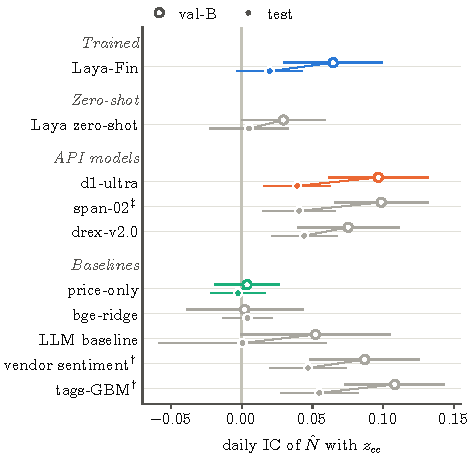
\includegraphics{fig1_validation_test.pdf}
\caption{\textbf{Every validation IC that is positive falls on test.} Daily IC of the pre-open news reading $\hat N$ with the close-to-close move $z_{cc}$, on (a) val-B and (b) the test period, on the same scale and one row per model, each with its 95\% interval ($\pm$1.96 Newey--West SE), for the instruments and the baselines (NA-12). Laya-Fin, the primary instrument, falls from 0.065 to 0.020; d1-ultra, the API comparator, from 0.097 to 0.039; span-02 and drex-v2.0 alike. The API models fail the \S{}8.3 contamination screens, so their results are model-specific (\S{}1.3). The clean benchmarks are about zero in both periods: price-only $-$0.003 and bge-ridge 0.004 on test; the LLM baseline, on a 2,000-event subsample, 0.001. The highest test ICs belong to the vendor-label baselines ($\dagger$: tags-GBM 0.055, vendor sentiment 0.047), whose labels were produced retrospectively: a possibly look-ahead-contaminated upper bound, not the benchmark. The anchor is uninformative (near-constant outputs); its ICs are in the appendix's model comparison. $\ddagger$ span-02: the S5 canary fired a STOP after the freeze and the operator chose to proceed (PREREG \S{}15, post-freeze NA-11 row).}\label{fig:fig1_validation_test}
\end{figure}

\clearpage

\section{Design: pre-registration, freeze, blinding, masking, ledgers}

\noindent\emph{No main figure or table; this section's are in the appendix.}

\clearpage

\section{Reading the news: priced at the open}

\begin{figure}[htbp]
\centering
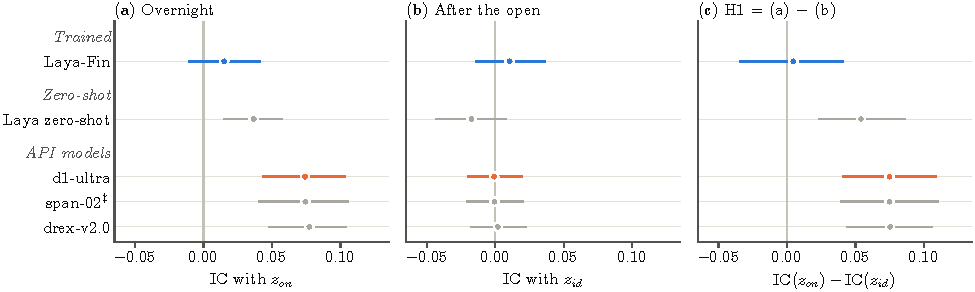
\includegraphics{fig2_priced_at_open.pdf}
\caption{\textbf{The API models' signal is priced at the open; no model predicts the move after it.} Daily IC of $\hat N$ on the test period with (a) the overnight move $z_{on}$ (previous close to open) and (b) the move after the open $z_{id}$ (open to close), with 95\% bootstrap intervals (NA-12); (c) H1, their difference, with its bootstrap interval. The three panels share one scale and one row per model. The API models' IC is all overnight: d1-ultra 0.074 with $z_{on}$ and $-$0.001 with $z_{id}$, H1 = 0.075 (p $<$0.001), model-specific (\S{}1.3); Laya zero-shot's H1 is 0.054. For Laya-Fin, the primary instrument, both ICs are small (0.015 and 0.010): H1 is not supported (Holm p 0.853) and so is H1b, the IC with $z_{id}$ (Holm p 0.853), although on val-B its IC with $z_{id}$ had been 0.054 (t 2.89; Table 2). The anchor is uninformative (near-constant outputs) and is in Table 1. $\ddagger$ span-02: the S5 canary fired a STOP after the freeze and the operator chose to proceed (PREREG \S{}15).}\label{fig:fig2_priced_at_open}
\end{figure}

% tab1_primary: tab:primary (NA-14 figures.latex, from artifacts/NA-12/tables/t1_primary.csv)
\begin{table}[htbp]
\centering
\small
\begin{threeparttable}
\caption{Primary hypotheses on the test period: none is supported for the primary instrument, Laya-Fin.}\label{tab:primary}
\begin{tabular}{@{}lS[table-format=-1.4]cS[table-format=1.3]S[table-format=1.3]S[table-format=-1.4]S[table-format=1.3]l@{}}
\toprule
 & \multicolumn{4}{c}{Laya-Fin (primary)} & \multicolumn{2}{c}{Anchor} & \\
\cmidrule(lr){2-5}\cmidrule(lr){6-7}
Hypothesis & {Estimate} & 95\% CI & {$p$} & {Holm $p$} & {Estimate} & {$p$} & Verdict (\S1.3) \\
\midrule
H1 & 0.005 & [$-0.035$, $0.041$] & 0.409 & 0.853 & 0.004 & 0.406 & not supported \\
H1b & 0.010 & [$-0.014$, $0.037$] & 0.213 & 0.853 & 0.002 & 0.427 & not supported \\
H2 & -0.044 & --- & 0.616 & 0.853 & 0.015 & 0.294 & not supported \\
H3 & 0.0038 & [$-0.0008$, $0.0085$] & 0.054 & 0.269 & 0.0013 & 0.017 & not supported \\
H4 & 0.0012 & [$-0.0017$, $0.0042$] & 0.216 & 0.853 & -0.0004 & 0.773 & not supported \\
\bottomrule
\end{tabular}
\begin{tablenotes}[flushleft]\footnotesize
\item The tests: H1, $\mathrm{IC}(\hat N, z_{on}) - \mathrm{IC}(\hat N, z_{id}) > 0$; H1b, $\mathrm{IC}(\hat N, z_{id}) > 0$; H2, $b > 0$ and $c < 0$ at D2; H3, $\Delta\mathrm{IC}$ of $J$ for $y_2 > 0$; H4, $\Delta R^2$ of the news for $|z_{cc}| > 0$.
\item Test period 2026-01-02 to 2026-07-31, events outside the embargo. Estimates in each hypothesis' direction; $p$ one-sided; 95\% CIs and $p$ from a stationary block bootstrap over sessions (block 5, 10,000 draws); Holm over H1, H1b, H2, H3 and H4 at 0.05.
\item H2: the estimate is $\min(b, -c)$ and $p = \max(p_b, p_c)$ (both must hold), so it has no single interval (---); $b$ and $c$ with their standard errors are in Table~\ref{tab:over-under}. Estimates and CIs to three decimals, H3's and H4's to four, since those increments are an order smaller.
\item Verdict (\S1.3): general if Laya-Fin's Holm $p < 0.05$ with the predicted sign and the anchor's own $p < 0.05$ with the same sign; model-specific if only Laya-Fin's holds; otherwise not supported. The anchor's readings are uninformative (near-constant outputs after one epoch); its rows are reported, not read as nulls. Its $p$ is its own, not Holm-adjusted.
\item Significance: no stars are used; $p$ is one-sided unless stated.
\end{tablenotes}
\end{threeparttable}
\end{table}


% tab2_ic_by_target: tab:ic-target (NA-14 figures.latex, from artifacts/NA-12/tables/t3_ic.csv, artifacts/NA-12/tables/t14_model_comparison.csv, artifacts/NA-14/tables/t32_val_b_ic.csv)
\begin{table}[htbp]
\centering
\small
\begin{threeparttable}
\caption{Daily IC by target: the API models' IC is 0.074 to 0.077 with the overnight move and about zero with the move after the open; no model predicts the move after the open.}\label{tab:ic-target}
\begin{tabular}{@{}lS[table-format=-1.3, table-space-text-pre=(, table-space-text-post=)]S[table-format=-1.3, table-space-text-pre=(, table-space-text-post=)]S[table-format=-1.3, table-space-text-pre=(, table-space-text-post=)]S[table-format=1.3, table-space-text-pre=(, table-space-text-post=)]S[table-format=1.3, table-space-text-pre=(, table-space-text-post=)]S[table-format=-1.3, table-space-text-pre=(, table-space-text-post=)]@{}}
\toprule
 & \multicolumn{3}{c}{Val-B} & \multicolumn{3}{c}{Test} \\
\cmidrule(lr){2-4}\cmidrule(lr){5-7}
Model & {$z_{cc}$} & {$z_{on}$} & {$z_{id}$} & {$z_{cc}$} & {$z_{on}$} & {$z_{id}$} \\
\midrule
\multicolumn{7}{@{}l}{\textit{Trained and zero-shot}} \\
Laya-Fin & 0.065 & 0.045 & 0.054 & 0.020 & 0.015 & 0.010 \\
 & {(}3.64{)} & {(}2.93{)} & {(}2.89{)} & {(}1.67{)} & {(}1.08{)} & {(}0.82{)} \\
anchor & -0.020 & -0.002 & -0.011 & 0.008 & 0.006 & 0.002 \\
 & {(}-1.52{)} & {(}-0.16{)} & {(}-0.75{)} & {(}0.83{)} & {(}0.50{)} & {(}0.18{)} \\
Laya zero-shot & 0.029 & 0.047 & 0.002 & 0.005 & 0.037 & -0.017 \\
 & {(}1.94{)} & {(}2.55{)} & {(}0.12{)} & {(}0.37{)} & {(}3.22{)} & {(}-1.25{)} \\
\addlinespace
\multicolumn{7}{@{}l}{\textit{API models (model-specific)}} \\
d1-ultra & 0.097 & {---} & {---} & 0.039 & 0.074 & -0.001 \\
 & {(}5.38{)} & {---} & {---} & {(}3.23{)} & {(}4.74{)} & {(}-0.07{)} \\
span-02$^{\ddagger}$ & 0.099 & {---} & {---} & 0.041 & 0.074 & -0.001 \\
 & {(}5.83{)} & {---} & {---} & {(}3.10{)} & {(}4.49{)} & {(}-0.05{)} \\
drex-v2.0 & 0.075 & {---} & {---} & 0.044 & 0.077 & 0.002 \\
 & {(}4.10{)} & {---} & {---} & {(}3.70{)} & {(}5.34{)} & {(}0.18{)} \\
\bottomrule
\end{tabular}
\begin{tablenotes}[flushleft]\footnotesize
\item Mean daily Spearman IC of the pre-open news reading $\hat N$ with the close-to-close move $z_{cc}$, the overnight move $z_{on}$ (previous close to open) and the move after the open $z_{id}$ (open to close), each in typical daily moves, to three decimals; Newey--West $t$ in parentheses, to two; D0 events outside the embargo (val-B 2025-10-01 to 2025-12-31; test 2026-01-02 to 2026-07-31).
\item Val-B ICs with $z_{on}$ and $z_{id}$ come from a run of the frozen specification on val-B before the freeze, which covered the trained and zero-shot Laya models only (---: not computed).
\item The anchor's readings are uninformative (near-constant outputs after one epoch); its rows are reported, not read as nulls. The API models fail the pre-registered contamination screens, so their results are model-specific. $^{\ddagger}$span-02: after the freeze, a stability check that repeats earlier requests (the canary) fired for it; its build was unchanged, and production went ahead under a rule recorded in the deviations log.
\end{tablenotes}
\end{threeparttable}
\end{table}


\clearpage

\section{Over- and under-reaction, and convergence to the news-implied value}

\begin{figure}[htbp]
\centering
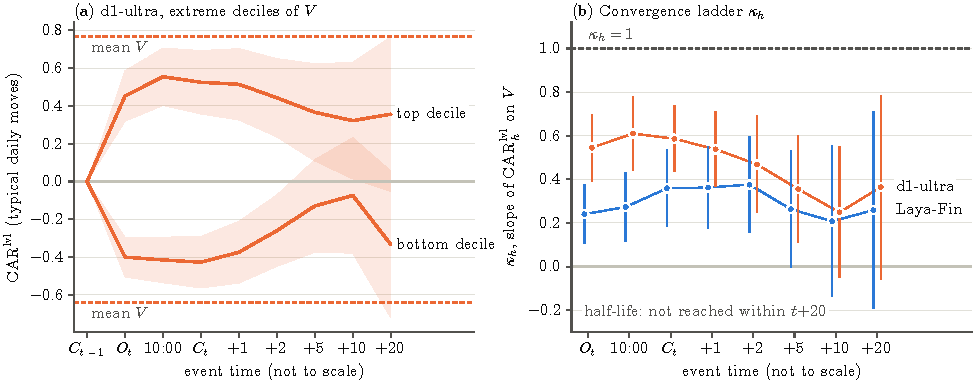
\includegraphics{fig3_convergence.pdf}
\caption{\textbf{Prices move part of the way to the model's value on day t, then partly fade.} Convergence to the news-implied value $V$ (PREREG A1), test period. Event time is not to scale: $O_t$ is the open, 10:00 the D1 decision point, $C_t$ the close of day $t$ and $+k$ the close of session $t+k$. (a) d1-ultra's top and bottom deciles of $V$: $\mathrm{CAR}^{\mathrm{lvl}}$, the abnormal return from the previous close in typical daily moves, with SE bands ($\pm$1.96 event-level SE; descriptive), against each decile's mean $V$ (dashed). The top decile (mean $V$ 0.77) stands at +0.45 at the open, +0.52 at the close and +0.36 at t+20; the bottom decile (mean $V$ $-$0.64) at $-$0.40, $-$0.43 and $-$0.33. Before the event prices drift in $V$'s direction (not drawn): five sessions earlier the top decile stood $-$1.19 and the bottom decile +1.54 from the previous close, so part of $V$ reflects momentum. The other deciles, and Laya-Fin's, are in Appendix Figure A7. (b) The convergence ladder $\kappa_h$, the slope of $\mathrm{CAR}^{\mathrm{lvl}}_h$ on $V$ with day $\times$ tier fixed effects, with 95\% intervals from two-way clustered SEs, against full convergence at $\kappa_h = 1$. $\kappa_h$ peaks on day $t$ or just after and is far from one: Laya-Fin 0.36 at the close and 0.38 at t+2, d1-ultra 0.61 at 10:00; it fades by t+10 (0.21 and 0.25). Laya-Fin's increase from the open to t+20 is +0.02 (p 0.467). The half-life of the gap $U = V - G^{\mathrm{lvl}}$, the first rung at which $\lambda_h$ reaches 0.5, is not reached within t+20 for any model ($\infty$; Table 4). The convergence tests (H2-C) are not supported after Benjamini--Hochberg. The anchor is uninformative (near-constant outputs) and appears in Figure A7. d1-ultra fails the \S{}8.3 screens and is model-specific (\S{}1.3).}\label{fig:fig3_convergence}
\end{figure}

\begin{figure}[htbp]
\centering
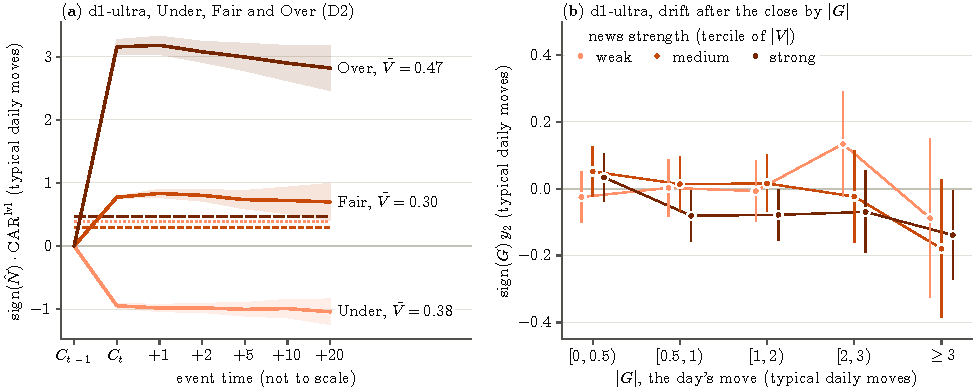
\includegraphics{fig4_over_under.pdf}
\caption{\textbf{No small-move underreaction; large moves reverse slightly.} Over- and under-reaction, test period (NA-12 figure data). (a) d1-ultra's D2 events by RG class, pooled over the tiers and signed in the news' direction ($\mathrm{sign}(\hat N)\cdot\mathrm{CAR}^{\mathrm{lvl}}$), with SE bands ($\pm$1.96 event-level SE), against each class's mean signed $V$ ($\bar V$ in the labels; dashed in the class's colour, dotted for Under, short dashes for Fair and long dashes for Over, since the three lie close). The 5,021 Under events moved against the news on day $t$ ($-$0.95) and never catch up ($-$1.04 at t+20, against a target of 0.38); the 1,783 Over events give back part of their move, from +3.16 at the close to +2.82. Laya-Fin has only 146 D2 events with $|\hat N| \geq 0.5$, too few to draw. (b) d1-ultra's drift after the close, $\mathrm{sign}(G)\,y_2$ (next open to the close of t+5, in the direction of the day's move $G$), by bin of $|G|$, one line per tercile of news strength, with 95\% intervals. The terciles are on $|V|$, Call A's value on the day's news (NA-12's figure data), not on $|\hat N|$. Moves with $|G| \geq 3$ reverse slightly in every tercile (strong $-$0.14, medium $-$0.18, weak $-$0.09); below that the means are small and of both signs, except the strong tercile, which also reverses slightly at 0.5 to 2 ($-$0.08 and $-$0.08). There is no small-move underreaction. Laya-Fin's panel is Appendix Figure A8. The pre-registered regression H2 finds, for Laya-Fin, b = $-$0.04 (p 0.616) and c = $-$0.015 (p 0.110): not supported (Table 3). d1-ultra is model-specific (\S{}1.3).}\label{fig:fig4_over_under}
\end{figure}

% tab3_over_under: tab:over-under (NA-14 figures.latex, from artifacts/NA-12/tables/t2_h2_over_under.csv)
\begin{table}[htbp]
\centering
\small
\begin{threeparttable}
\caption{The over/under regression: the reversal coefficient $c$ has the predicted sign but is not significant, and the news coefficient $b$ is not positive at the close.}\label{tab:over-under}
\begin{tabular}{@{}lS[table-format=-1.3]S[table-format=1.3, table-space-text-pre=(, table-space-text-post=)]S[table-format=1.3]S[table-format=-1.3]S[table-format=1.3, table-space-text-pre=(, table-space-text-post=)]S[table-format=1.3]S[table-format=5.0]@{}}
\toprule
Decision point & {$b$} & {SE} & {$p_b$} & {$c$} & {SE} & {$p_c$} & {Events} \\
\midrule
\multicolumn{8}{@{}l}{\textit{Laya-Fin (primary)}} \\
D2, close (H2) & -0.044 & {(}0.149{)} & 0.616 & -0.015 & {(}0.012{)} & 0.110 & 17188 \\
D1, 10:00 & 0.229 & {(}0.148{)} & 0.062 & 0.013 & {(}0.012{)} & 0.861 & 13203 \\
D0, open & 0.278 & {(}0.212{)} & 0.096 & {---} & {---} & {---} & 13439 \\
\addlinespace
\multicolumn{8}{@{}l}{\textit{Anchor (uninformative)}} \\
D2, close (H2) & 0.748 & {(}1.377{)} & 0.294 & -0.015 & {(}0.012{)} & 0.111 & 17188 \\
D1, 10:00 & 1.964 & {(}2.482{)} & 0.215 & 0.014 & {(}0.012{)} & 0.874 & 13203 \\
D0, open & -4.510 & {(}3.236{)} & 0.917 & {---} & {---} & {---} & 13439 \\
\addlinespace
\multicolumn{8}{@{}l}{\textit{d1-ultra (model-specific)}} \\
D2, close (H2) & -0.076 & {(}0.031{)} & 0.991 & -0.011 & {(}0.012{)} & 0.171 & 17188 \\
D1, 10:00 & -0.018 & {(}0.032{)} & 0.711 & 0.015 & {(}0.012{)} & 0.884 & 13203 \\
D0, open & 0.022 & {(}0.037{)} & 0.277 & {---} & {---} & {---} & 13439 \\
\bottomrule
\end{tabular}
\begin{tablenotes}[flushleft]\footnotesize
\item $y = a + b\,\hat N + c\,G$ with day $\times$ tier fixed effects, on the test period: at D2 $y = y_2$ (next open to $t{+}5$), $\hat N$ from the day's news and $G$ the day's move; at D1 the move after 10:00 on $\hat N$ from the pre-open news and the move to 10:00; at D0 $y = z_{id}$ and there is no $G$. Two-way clustered (session, firm) standard errors in parentheses; $p_b$ tests $b > 0$ and $p_c$ tests $c < 0$, one-sided. H2 is the D2 row of Laya-Fin.
\item The anchor's readings are uninformative (near-constant outputs after one epoch); its rows are reported, not read as nulls. The API models fail the \S8.3 contamination screens, so their results are model-specific (\S1.3).
\item Significance: no stars are used; $p$ is one-sided unless stated.
\end{tablenotes}
\end{threeparttable}
\end{table}


% tab4_convergence: tab:convergence (NA-14 figures.latex, from artifacts/NA-12/tables/t6_convergence_ladder.csv, artifacts/NA-12/tables/t7_gap_closure.csv)
\begin{table}[htbp]
\centering
\small
\setlength{\tabcolsep}{4pt}
\begin{threeparttable}
\caption{Convergence to the news-implied value $V$: prices reach part of $V$ on day $t$ ($\kappa$ at the close 0.36 for Laya-Fin and 0.59 for d1-ultra), then partly fade; the gap's half-life is not reached within $t{+}20$.}\label{tab:convergence}
\begin{tabular}{@{}lS[table-format=1.2, table-space-text-pre=(, table-space-text-post=)]S[table-format=-1.2, table-space-text-pre=(, table-space-text-post=)]S[table-format=-1.3, table-space-text-pre=(, table-space-text-post=)]S[table-format=-1.3, table-space-text-pre=(, table-space-text-post=)]S[table-format=-1.2, table-space-text-pre=(, table-space-text-post=)]S[table-format=-1.3, table-space-text-pre=(, table-space-text-post=)]S[table-format=-1.2, table-space-text-pre=(, table-space-text-post=)]S[table-format=-1.3, table-space-text-pre=(, table-space-text-post=)]S[table-format=1.0]@{}}
\toprule
 & {$O_t$} & {10:00} & {$C_t$} & {$t{+}1$} & {$t{+}2$} & {$t{+}5$} & {$t{+}10$} & {$t{+}20$} & {Half-life} \\
\midrule
\multicolumn{10}{@{}l}{\textit{Panel A: convergence ladder $\kappa_h$ (D0 events)}} \\
Laya-Fin & 0.24 & 0.27 & 0.36 & 0.36 & 0.38 & 0.26 & 0.21 & 0.26 & {---} \\
 & {(}0.07{)} & {(}0.08{)} & {(}0.09{)} & {(}0.10{)} & {(}0.11{)} & {(}0.14{)} & {(}0.18{)} & {(}0.23{)} & {---} \\
d1-ultra & 0.55 & 0.61 & 0.59 & 0.54 & 0.47 & 0.36 & 0.25 & 0.36 & {---} \\
 & {(}0.08{)} & {(}0.09{)} & {(}0.08{)} & {(}0.09{)} & {(}0.11{)} & {(}0.13{)} & {(}0.15{)} & {(}0.22{)} & {---} \\
anchor & 0.08 & -0.02 & -0.04 & -0.04 & -0.03 & -0.06 & -0.03 & 0.08 & {---} \\
 & {(}0.08{)} & {(}0.08{)} & {(}0.07{)} & {(}0.09{)} & {(}0.09{)} & {(}0.10{)} & {(}0.11{)} & {(}0.16{)} & {---} \\
\addlinespace
\multicolumn{10}{@{}l}{\textit{Panel B: gap closure $\lambda_h$ and the half-life}} \\
Laya-Fin, D2 & {---} & {---} & {---} & -0.007 & {---} & 0.026 & {---} & 0.050 & {$\infty$} \\
 & {---} & {---} & {---} & {(}0.012{)} & {---} & {(}0.026{)} & {---} & {(}0.051{)} & {---} \\
Laya-Fin, D1 & {---} & {---} & -0.011 & -0.024 & {---} & -0.002 & {---} & -0.013 & {$\infty$} \\
 & {---} & {---} & {(}0.013{)} & {(}0.020{)} & {---} & {(}0.034{)} & {---} & {(}0.062{)} & {---} \\
d1-ultra, D2 & {---} & {---} & {---} & -0.009 & {---} & 0.022 & {---} & 0.049 & {$\infty$} \\
 & {---} & {---} & {---} & {(}0.012{)} & {---} & {(}0.026{)} & {---} & {(}0.051{)} & {---} \\
d1-ultra, D1 & {---} & {---} & -0.013 & -0.028 & {---} & -0.012 & {---} & -0.020 & {$\infty$} \\
 & {---} & {---} & {(}0.013{)} & {(}0.020{)} & {---} & {(}0.034{)} & {---} & {(}0.062{)} & {---} \\
anchor, D2 & {---} & {---} & {---} & -0.007 & {---} & 0.027 & {---} & 0.052 & {$\infty$} \\
 & {---} & {---} & {---} & {(}0.012{)} & {---} & {(}0.027{)} & {---} & {(}0.051{)} & {---} \\
anchor, D1 & {---} & {---} & -0.012 & -0.025 & {---} & -0.003 & {---} & -0.013 & {$\infty$} \\
 & {---} & {---} & {(}0.013{)} & {(}0.020{)} & {---} & {(}0.034{)} & {---} & {(}0.062{)} & {---} \\
\bottomrule
\end{tabular}
\begin{tablenotes}[flushleft]\footnotesize
\item Panel A: $\kappa_h$ is the slope of $\mathrm{CAR}^{\mathrm{lvl}}_h$, the abnormal return from the previous close to rung $h$ in typical daily moves, on $V$ with day $\times$ tier fixed effects; $\kappa_h = 1$ is full convergence. Panel B: $\lambda_h$ is the share of the gap $U = V - G^{\mathrm{lvl}}$ closed by rung $h$, at D2 (from the close) and D1 (from 10:00); the half-life is the first rung with $\lambda_h \geq 0.5$ ($\infty$: not reached within $t{+}20$). Two-way clustered standard errors in parentheses; $t{+}k$ is the close of session $t+k$. ---: not estimated; $\lambda_h$ is reported at $t{+}1$, $t{+}5$ and $t{+}20$ from D2 and also at $C_t$ from D1, and the half-life belongs to $\lambda_h$ alone. $\kappa_h$ to two decimals, $\lambda_h$ to three, since it is an order smaller.
\item The anchor's readings are uninformative (near-constant outputs after one epoch); its rows are reported, not read as nulls. The API models fail the pre-registered contamination screens, so their results are model-specific.
\end{tablenotes}
\end{threeparttable}
\end{table}


\clearpage

\section{Explaining realized moves}

\begin{figure}[htbp]
\centering
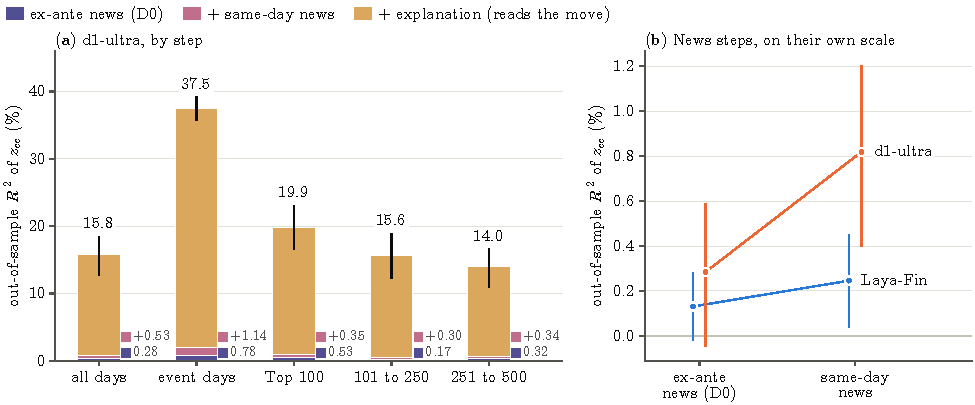
\includegraphics{fig5_explaining_moves.pdf}
\caption{\textbf{The news explains little of a stock's own move; reading the move explains more.} Explaining realized moves at the firm level (PREREG A3, after Kelly--Su--Zhang), test period (NA-12), as out-of-sample $R^2$ in \% of the stock-specific variance. (a) d1-ultra's $R^2$ of the stock-specific move $z_{cc}$ by cut, stacked by step in the order of the legend: the ex-ante (D0) news, + the same-day news (Call A), + the explanation (Call B reads the realized move, so this step is not a prediction). The total stands above each bar with its 95\% bootstrap interval: 15.8\% of all covered member-days and 37.5\% of event days. The two news steps are too thin to read, so their values stand beside each bar after a swatch of their colour: the ex-ante step's $R^2$, then the same-day step's increment. For comparison, the market and the sector, Roll's first step, explain 25.3\% of total daily variance, a different base. (b) The news steps on their own scale, the zoom that makes them readable: the $R^2$ after the ex-ante and after the same-day news, with 95\% bootstrap intervals. Laya-Fin's same-day news explains 0.25\% of the stock-specific variance, the only secondary test that survives Benjamini--Hochberg (H5, q 0.058), and 0.13\% was knowable before the open; d1-ultra's steps reach 0.82\% and 0.28\%. The trained models give no explanation answer; the anchor is uninformative (near-constant outputs; Table 5). d1-ultra is model-specific (\S{}1.3).}\label{fig:fig5_explaining_moves}
\end{figure}

% tab5_explaining_moves: tab:explaining (NA-14 figures.latex, from artifacts/NA-12/tables/t10_explanation_ladder.csv, artifacts/NA-12/tables/t4_secondary.csv)
\begin{table}[htbp]
\centering
\small
\begin{threeparttable}
\caption{Explaining realized moves: same-day news explains 0.25\% of the stock-specific variance for Laya-Fin (H5, supported) and 0.82\% for d1-ultra; reading the move explains 15.8\%.}\label{tab:explaining}
\begin{tabular}{@{}lS[table-format=2.3]S[table-format=1.2]S[table-format=2.3, table-space-text-pre={$<$}]S[table-format=2.2]S[table-format=2.3]S[table-format=1.2]@{}}
\toprule
 & \multicolumn{2}{c}{Laya-Fin} & \multicolumn{2}{c}{d1-ultra} & \multicolumn{2}{c}{Anchor} \\
\cmidrule(lr){2-3}\cmidrule(lr){4-5}\cmidrule(lr){6-7}
Step & {$R^2$} & {$\Delta R^2$} & {$R^2$} & {$\Delta R^2$} & {$R^2$} & {$\Delta R^2$} \\
\midrule
\multicolumn{7}{@{}l}{\textit{Panel A: the explanation ladder, out-of-sample $R^2$ of $z_{cc}$ (\%)}} \\
+ ex-ante news (D0) & 0.13 & {---} & 0.28 & {---} & 0.01 & {---} \\
+ same-day news & 0.25 & 0.12 & 0.82 & 0.53 & 0.03 & 0.02 \\
+ explanation (reads the move) & {---} & {---} & 15.76 & 14.94 & {---} & {---} \\
share knowable before the open (\%) & 53.17 & {---} & 34.78 & {---} & 35.63 & {---} \\
\addlinespace
\multicolumn{7}{@{}l}{\textit{Panel B: the secondary test H5}} \\
H5: same-day news step, $R^2 > 0$ & 0.25 & {---} & 0.82 & {---} & 0.03 & {---} \\
one-sided $p$ & 0.010 & {---} & {$<$}0.001 & {---} & 0.072 & {---} \\
BH $q$ & 0.058 & {---} & {$<$}0.001 & {---} & 0.358 & {---} \\
\bottomrule
\end{tabular}
\begin{tablenotes}[flushleft]\footnotesize
\item Covered member-days of the test period; out-of-sample $R^2$ of the stock-specific move $z_{cc}$ (the market and sector removed) by cumulative step, in \%; $\Delta R^2$ is the step's increment. Roll's first step, the market and the sector, explains 25.3\% of total daily variance, a different base. The explanation step needs the post-reaction reading's explanation answer, which only d1-ultra gives; it reads the realized move, so it is not a prediction. H5 is the only secondary test that survives Benjamini--Hochberg ($q$ 0.10) for Laya-Fin. ---: not applicable (the first step has no increment; only d1-ultra answers the explanation question; the share and Panel B have one value per model). $R^2$, $\Delta R^2$ and the share in \% to two decimals; $p$ and $q$ to three.
\item The anchor's readings are uninformative (near-constant outputs after one epoch); its rows are reported, not read as nulls. The API models fail the pre-registered contamination screens, so their results are model-specific.
\end{tablenotes}
\end{threeparttable}
\end{table}


\clearpage

\section{Economic significance}

\begin{figure}[htbp]
\centering
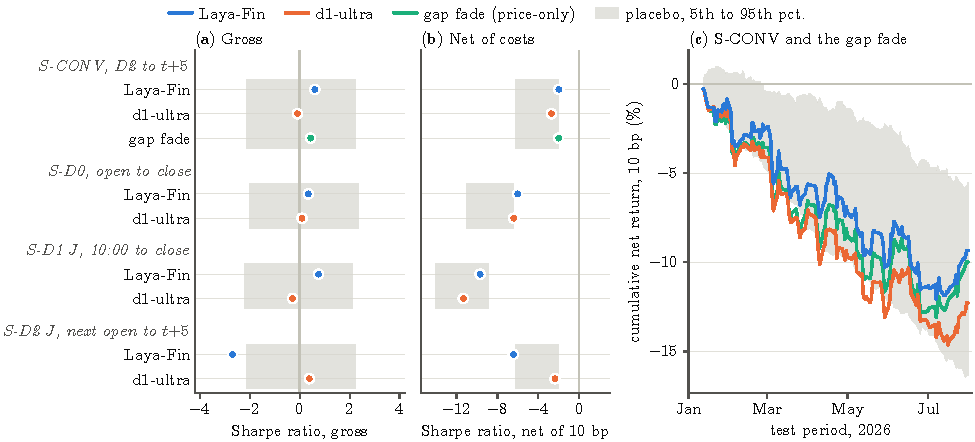
\includegraphics{fig6_strategies.pdf}
\caption{\textbf{No pre-registered book survives costs and the deflated Sharpe; S-CONV is effectively the gap fade.} Strategies on the test period (NA-13). (a, b) Annualized Sharpe ratio of each main book, gross and net of 10 bp per side on both legs and the SPY hedge, at the exit of its hypothesis' horizon; the gray box is the 5th to 95th percentile of the book's 100 random-signal books; (b) has its own scale. Gross, no book reaches the top of its placebo range (S-CONV's: $-$2.12 to +2.23), and Laya-Fin's S-D2 $J$ falls below its bottom (placebo percentile 3); net, every one is negative (Laya-Fin's S-CONV $-$1.98, gross +0.61; S-D0 $-$6.03; S-D1 $J$ $-$9.70). The one-day books lose most to costs: they turn over 4.36 times their capital a day against 0.90 for S-CONV. (c) S-CONV's cumulative net return at 10 bp against the price-only gap fade, with the placebo's 5th to 95th percentile band. S-CONV is effectively the gap fade, because $V$ is small next to $G$ ($U \approx -G^{\mathrm{lvl}}$): the two share 92\% of their positions, 99.8\% of them on the same side, and their daily returns correlate 0.96. The only books positive net are Laya-Fin's RG books, with 6 to 12 positions over the whole test period, and the anchor's gated S-D2 $J$ held to t+20 (the anchor is uninformative, with near-constant outputs); none clears its placebo or the deflated Sharpe. The highest gross Sharpe, the gated S-D0 held to the close of t+1 (1.88), reaches placebo percentile 93; with the 545 trials in the ledger when NA-13 computed it, the largest deflated-Sharpe probability of any test book is 0.024. Every book is in the appendix's strategy table, the other books' paths and the tier sub-books in Figure A12. Borrow costs are not modelled.}\label{fig:fig6_strategies}
\end{figure}

% tab6_strategies: tab:strategies (NA-14 figures.latex, from artifacts/NA-14/tables/t20_strategies.csv, artifacts/NA-14/tables/t35_break_even.csv)
\begin{table}[htbp]
\centering
\small
\setlength{\tabcolsep}{3pt}
\begin{threeparttable}
\caption{Strategies on the test period: no pre-registered book survives costs and the deflated Sharpe ratio.}\label{tab:strategies}
\begin{tabular}{@{}llS[table-format=-1.2]S[table-format=-2.2]S[table-format=1.2]S[table-format=-2.1]S[table-format=2.0]S[table-format=1.3, table-space-text-pre={$<$}]@{}}
\toprule
 & & \multicolumn{2}{c}{Sharpe ratio} & & & & \\
\cmidrule(lr){3-4}
Book & Holding & {Gross} & {Net} & {Turnover} & {Break-even (bp)} & {Placebo pct.} & {DSR} \\
\midrule
\multicolumn{8}{@{}l}{\textit{Laya-Fin (primary)}} \\
S-CONV & D2 to $t{+}5$ & 0.61 & -1.98 & 0.90 & 2.4 & 68 & {$<$}0.001 \\
S-D0 & open to close & 0.35 & -6.03 & 4.36 & 0.5 & 64 & {$<$}0.001 \\
S-D0, gated & open to $t{+}1$ & 1.88 & -0.38 & 2.31 & 8.3 & 93 & {$<$}0.001 \\
S-D1 $J$ & 10:00 to close & 0.76 & -9.70 & 4.36 & 0.7 & 71 & {$<$}0.001 \\
S-D2 $J$ & next open to $t{+}5$ & -2.69 & -6.45 & 0.83 & -7.1 & 3 & {$<$}0.001 \\
S-D2 RG & next open to $t{+}5$ & 1.69 & 1.50 & 0.05 & 85.1 & 92 & 0.024 \\
\addlinespace
\multicolumn{8}{@{}l}{\textit{d1-ultra (model-specific)}} \\
S-CONV & D2 to $t{+}5$ & -0.09 & -2.72 & 0.90 & -0.3 & 48 & {$<$}0.001 \\
S-D0 & open to close & 0.10 & -6.41 & 4.41 & 0.1 & 58 & {$<$}0.001 \\
S-D1 $J$ & 10:00 to close & -0.28 & -11.35 & 4.51 & -0.3 & 40 & {$<$}0.001 \\
S-D2 $J$ & next open to $t{+}5$ & 0.39 & -2.37 & 0.85 & 1.4 & 64 & {$<$}0.001 \\
\addlinespace
\multicolumn{8}{@{}l}{\textit{Benchmarks}} \\
gap fade (price-only) & D2 to $t{+}5$ & 0.44 & -2.01 & 0.90 & 1.8 & 66 & {$<$}0.001 \\
vendor sentiment$^{\dagger}$ & open to close & 0.27 & -6.24 & 4.36 & 0.4 & 62 & {$<$}0.001 \\
\bottomrule
\end{tabular}
\begin{tablenotes}[flushleft]\footnotesize
\item Annualized Sharpe ratios ($\sqrt{252}$), gross and net of 10 bp per side on both legs and the SPY hedge; no borrow cost. Turnover: dollars traded a day per dollar of capital. Break-even: the cost per side, in basis points, at which the mean net return is zero (gross mean $\div$ turnover). Placebo: the percentile of the gross Sharpe among 100 random-signal books on the same events. DSR: the deflated-Sharpe probability at 10 bp with the 545 trials of the trials ledger. Each family is shown at its hypothesis' horizon; every book is in Table~\ref{tab:a-strategies}. S-CONV ranks by the gap $U = V - G^{\mathrm{lvl}}$; S-D0 by $\tilde N$; S-D1 and S-D2 by the judgment $J$ signed by the move; RG books trade the cases the model calls a misreaction (one name a side).
\item $^{\dagger}$Vendor-label baseline (vendor sentiment, tags-GBM): the labels were produced retrospectively, so its IC is a possibly look-ahead-contaminated upper bound, not the benchmark; the clean benchmarks are bge-ridge, price-only, the LLM baseline and the random-signal placebo. The API models fail the \S8.3 contamination screens, so their results are model-specific (\S1.3).
\end{tablenotes}
\end{threeparttable}
\end{table}


\clearpage

\section{Memorisation and validation-to-test decay}

\begin{figure}[htbp]
\centering
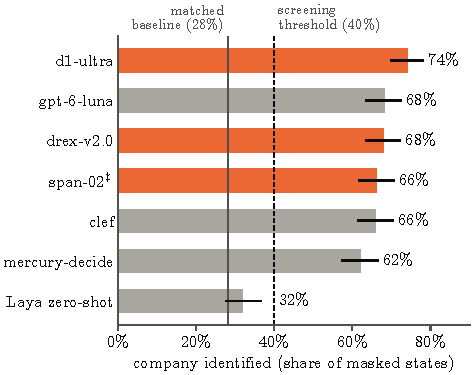
\includegraphics{fig7_memorisation.pdf}
\caption{\textbf{The API models identify the masked company; Laya zero-shot hardly does.} Company identification on masked val-A states with activity-matched distractors (NA-11; the \S{}8.3 screen): the share of states in which each model names the company among four candidates, as a bar, sorted, with its Wilson 95\% interval and its value at the bar's end, against the matched baseline (a no-reading guess, 28\%; solid) and the screening threshold (40\%; dashed). The production comparators (d1-ultra, span-02, drex-v2.0) are in the comparator colour, the other API models and Laya zero-shot in gray. The API models name it in 62\% to 74\% of states, so they fail the screen and are model-specific (\S{}1.3); Laya zero-shot, Laya-Fin's base, names it in 32\%. Every model was released after the sample, which ends on 2026-07-31: Laya's open weights on 2026-09-18 (49 days later; the operator's date) and the API models between 2026-10-12 and 2026-10-16 (NA-05 catalog). Identifying a company is not the same as remembering its returns, and the test does not settle that. $\ddagger$ span-02: the S5 canary fired a STOP after the freeze and the operator chose to proceed (PREREG \S{}15).}\label{fig:fig7_memorisation}
\end{figure}

\clearpage

\appendix

\renewcommand{\thefigure}{A\arabic{figure}}\setcounter{figure}{0}

\renewcommand{\thetable}{A\arabic{table}}\setcounter{table}{0}

\section{Decision models}

\begin{figure}[htbp]
\centering
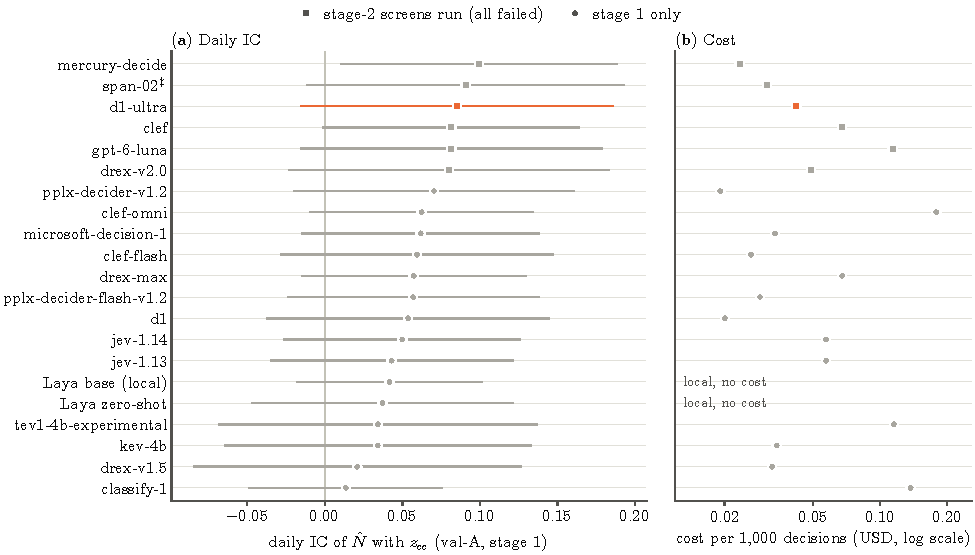
\includegraphics{figA1_tournament.pdf}
\caption{\textbf{The zero-shot tournament.} The zero-shot tournament on NA-06's val-A stage-1 sample: (a) the daily IC of Call A's $\hat N$ with $z_{cc}$ and its 95\% bootstrap interval, models sorted by IC; (b) the cost per 1,000 decisions (log scale; the local Laya models cost nothing). Every model is in the model confidence set; the highest IC is mercury-decide's (0.099) and d1-ultra's is 0.085. The six models that ran the stage-2 screens (squares) all failed them (Figure 7). $\ddagger$ span-02: the S5 canary fired a STOP after the freeze and the operator chose to proceed (PREREG \S{}15).}\label{fig:figA1_tournament}
\end{figure}

\clearpage

% t14_model_comparison (NA-14, from artifacts/NA-12/tables/t14_model_comparison.csv)
\begin{table*}[tbp]
\centering\small
\caption{Model comparison: daily IC of \^{N}\_W0 with z\_cc (val-B, test, common test events), cost, latency}\label{tab:t14_model_comparison}
\begin{adjustbox}{max width=\textwidth}
\begin{tabular}{ll>{\raggedright\arraybackslash}p{12em}rrrrrrrrrrrrr>{\raggedright\arraybackslash}p{12em}}
\toprule
model & name & role & IC val-B & IC val-B t & IC val-B n & IC test & IC test t & IC test n & IC common & IC common t & IC common n & cost per 1000 & latency p50 ms & latency p95 ms & coverage & footnote \\
\midrule
Laya-Fin & Laya-Fin & primary instrument (laya-s13) & $0.065$ & $3.642$ & $5{,}506$ & $0.020$ & $1.671$ & $13{,}748$ & $0.020$ & $1.671$ & $13{,}748$ & $0.000$ & --- & --- & $1.000$ & --- \\
anchor (uninformative) & anchor (uninformative) & clean anchor (anchor-s13) & $-0.020$ & $-1.517$ & $5{,}506$ & $0.008$ & $0.826$ & $13{,}748$ & $0.008$ & $0.826$ & $13{,}748$ & $0.000$ & --- & --- & $1.000$ & --- \\
Laya zero-shot & local/laya-typed-decisions & Laya zero-shot (PREREG \S{}10.5) & $0.029$ & $1.938$ & $5{,}506$ & $0.005$ & $0.369$ & $13{,}748$ & $0.005$ & $0.369$ & $13{,}748$ & $0.000$ & $535.794$ & $757.822$ & $1.000$ & --- \\
d1-ultra & liquid/d1-ultra & best API comparator; screen-failing, model-specific & $0.097$ & $5.377$ & $5{,}506$ & $0.039$ & $3.229$ & $13{,}748$ & $0.039$ & $3.229$ & $13{,}748$ & $0.063$ & $287.912$ & $427.372$ & $1.000$ & --- \\
span-02\textsuperscript{\ddag} & respan/span-02\textsuperscript{\ddag} & core comparator; screen-failing, model-specific & $0.099$ & $5.829$ & $5{,}506$ & $0.041$ & $3.098$ & $13{,}748$ & $0.041$ & $3.098$ & $13{,}748$ & $0.028$ & $2261.997$ & $2458.838$ & $1.000$ & S5 canary STOP, operator:\allowbreak{} proceed (PREREG \S{}15, post-freeze NA-11 row) \\
drex-v2.0 & nace-ai/drex-v2.0 & core comparator; screen-failing, model-specific & $0.075$ & $4.099$ & $5{,}506$ & $0.044$ & $3.696$ & $13{,}748$ & $0.044$ & $3.696$ & $13{,}748$ & $0.045$ & $679.966$ & $1115.333$ & $1.000$ & --- \\
vendor sentiment\textsuperscript{\dag} & --- & baseline (PREREG \S{}10) & $0.087$ & $4.389$ & $5{,}506$ & $0.047$ & $3.364$ & $13{,}748$ & --- & --- & --- & --- & --- & --- & --- & --- \\
bge-ridge & --- & baseline (PREREG \S{}10) & $0.002$ & $0.103$ & $5{,}506$ & $0.004$ & $0.447$ & $13{,}748$ & --- & --- & --- & --- & --- & --- & --- & --- \\
tags-GBM\textsuperscript{\dag} & --- & baseline (PREREG \S{}10) & $0.108$ & $6.025$ & $5{,}506$ & $0.055$ & $3.913$ & $13{,}748$ & --- & --- & --- & --- & --- & --- & --- & --- \\
LLM baseline & --- & baseline (PREREG \S{}10) & $0.052$ & $1.928$ & $1{,}978$ & $5.47\times 10^{-4}$ & $0.018$ & $1{,}977$ & --- & --- & --- & --- & --- & --- & --- & --- \\
price-only & --- & baseline (PREREG \S{}10) & $0.004$ & $0.331$ & $5{,}506$ & $-0.003$ & $-0.263$ & $13{,}748$ & --- & --- & --- & --- & --- & --- & --- & --- \\
Laya-Fin & --- & the LLM baseline's test subsample & --- & --- & --- & $-0.012$ & $-0.371$ & $1{,}977$ & --- & --- & --- & --- & --- & --- & --- & --- \\
LLM baseline & --- & the LLM baseline's test subsample & --- & --- & --- & $5.47\times 10^{-4}$ & $0.018$ & $1{,}977$ & --- & --- & --- & --- & --- & --- & --- & --- \\
price\_only (D2, y2) & --- & baseline (PREREG \S{}10.4) & --- & --- & --- & $0.012$ & $1.177$ & $17{,}188$ & --- & --- & --- & --- & --- & --- & --- & --- \\
\bottomrule
\end{tabular}
\end{adjustbox}
\par\smallskip{\footnotesize\raggedright The API models are screen-failing and model-specific (\S{}15 NA-06 row). span-02: the S5 canary fired a STOP and the operator chose to proceed (PREREG \S{}15, post-freeze NA-11 row). Costs per 1,000 decisions include answers paid by earlier chunks; the price-only D2 row is IC with y2. \textsuperscript{\dag} Vendor-label baseline (vendor sentiment, tags-GBM): the labels were produced retrospectively (CLAUDE.md A6), so this row is a possibly look-ahead-contaminated upper bound, not the benchmark. The clean benchmarks are bge-ridge, price-only, the LLM baseline and the random-signal placebo. The anchor's readings are uninformative (near-constant outputs: NA-11 REPORT \S{}7.1 item 4); its rows are reported, not read as nulls.\par}
\end{table*}


\clearpage

% t27_tournament (NA-14, from artifacts/NA-06/fig3_data.csv)
\begin{table*}[tbp]
\centering\small
\caption{NA-06 zero-shot tournament (val-A stage-1 sample): daily IC, cost per 1,000 decisions, MCS membership, \S{}8.3 screens}\label{tab:t27_tournament}
\begin{adjustbox}{max width=\textwidth}
\begin{tabular}{>{\raggedright\arraybackslash}p{12em}lrrrrlll}
\toprule
model & kind & cost per 1000 decisions & IC & CI low & CI high & MCS member & stage2 & screen \\
\midrule
inception/mercury-decide & api & $0.023$ & $0.099$ & $0.010$ & $0.189$ & yes & yes & fail \\
respan/span-02\textsuperscript{\ddag} & api & $0.031$ & $0.091$ & $-0.012$ & $0.193$ & yes & yes & fail \\
liquid/d1-ultra & api & $0.042$ & $0.085$ & $-0.016$ & $0.186$ & yes & yes & fail \\
cloudflare/clef & api & $0.068$ & $0.082$ & $-0.001$ & $0.164$ & yes & yes & fail \\
openai/gpt-6-luna-decisions & api & $0.114$ & $0.081$ & $-0.016$ & $0.179$ & yes & yes & fail \\
nace-ai/drex-v2.0 & api & $0.049$ & $0.080$ & $-0.024$ & $0.183$ & yes & yes & fail \\
perplexity/pplx-decider-v1.2 & api & $0.019$ & $0.070$ & $-0.020$ & $0.161$ & yes & no & not\_tested \\
cloudflare/clef-omni & api & $0.180$ & $0.062$ & $-0.010$ & $0.135$ & yes & no & not\_tested \\
microsoft/microsoft-decision-1 & api & $0.034$ & $0.062$ & $-0.015$ & $0.138$ & yes & no & not\_tested \\
cloudflare/clef-flash & api & $0.026$ & $0.059$ & $-0.028$ & $0.147$ & yes & no & not\_tested \\
nace-ai/drex-max & api & $0.068$ & $0.057$ & $-0.015$ & $0.130$ & yes & no & not\_tested \\
perplexity/pplx-decider-flash-v1.2 & api & $0.029$ & $0.057$ & $-0.024$ & $0.138$ & yes & no & not\_tested \\
liquid/d1 & api & $0.020$ & $0.054$ & $-0.037$ & $0.145$ & yes & no & not\_tested \\
typesafe/jev-1.14 & api & $0.057$ & $0.050$ & $-0.026$ & $0.126$ & yes & no & not\_tested \\
typesafe/jev-1.13 & api & $0.057$ & $0.043$ & $-0.035$ & $0.121$ & yes & no & not\_tested \\
local/laya-base & local & $0.000$ & $0.042$ & $-0.018$ & $0.101$ & yes & no & not\_tested \\
local/laya-typed-decisions & local & $0.000$ & $0.037$ & $-0.047$ & $0.121$ & yes & no & not\_tested \\
togethercomputer/tev1-4b-experimental & api & $0.116$ & $0.034$ & $-0.069$ & $0.137$ & yes & no & not\_tested \\
jaredpalmer/kev-4b & api & $0.034$ & $0.034$ & $-0.065$ & $0.133$ & yes & no & not\_tested \\
nace-ai/drex-v1.5 & api & $0.033$ & $0.021$ & $-0.085$ & $0.127$ & yes & no & not\_tested \\
scaledown/classify-1 & api & $0.138$ & $0.014$ & $-0.049$ & $0.076$ & yes & no & not\_tested \\
\bottomrule
\end{tabular}
\end{adjustbox}
\par\smallskip{\footnotesize\raggedright \textsuperscript{\ddag} span-02: the S5 canary fired a STOP after the freeze; the operator chose to proceed (PREREG \S{}15, the post-freeze NA-11 S5 row).\par}
\end{table*}


\clearpage

\section{Design}

\begin{figure}[htbp]
\centering
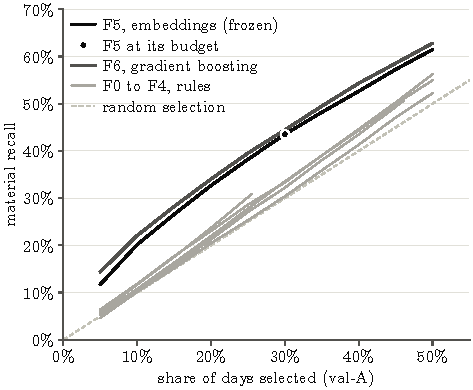
\includegraphics{figA2_filters.pdf}
\caption{\textbf{An embedding filter selects material news better than rule filters.} Material recall against the share of val-A days selected, per candidate importance filter (NA-03 frontier, budgets from 5\% to 50\% of days). The frozen filter F5, a logistic regression on bge-small embeddings, selects 30\% of days at its budget with material recall 0.435. F6 (gradient boosting) reaches 0.444 at the same budget, a tie within one point that goes to the filter with fewer inputs (\S{}6.8). The rule filters F1 to F4 recall 0.309 to 0.335 there, close to random selection (dashed); F0 keeps every clean article.}\label{fig:figA2_filters}
\end{figure}

\clearpage

\begin{figure}[htbp]
\centering
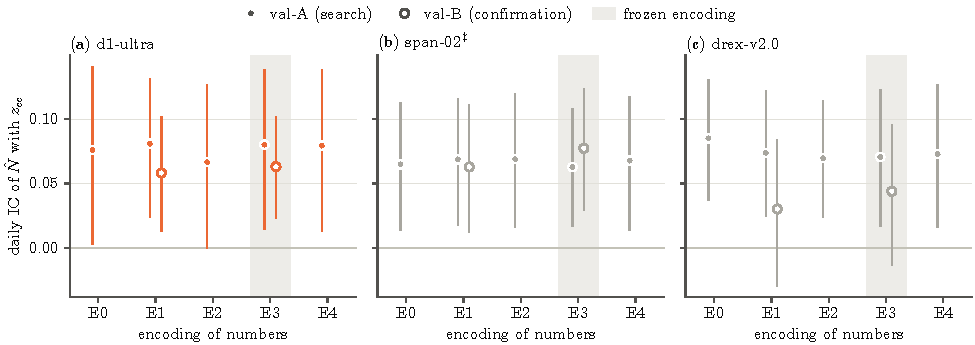
\includegraphics{figA3_encoding.pdf}
\caption{\textbf{How numbers are written in the state hardly matters.} The encoding of numbers in states (NA-07; \S{}8.4): daily IC of $\hat N$ with $z_{cc}$ by encoding E0 to E4 on NA-07's val-A sample (filled, 95\% bootstrap intervals) and the val-B confirmation of E1 and E3 (hollow), for the three API comparators; the gray column is the frozen encoding. E1 had the best mean val-A rank (1.67) but fell short of E3 on val-B by more than one standard error, so NA-07's rule kept E3 (d1-ultra on val-B: 0.058 with E1, 0.063 with E3). $\ddagger$ span-02: the S5 canary fired a STOP after the freeze and the operator chose to proceed (PREREG \S{}15).}\label{fig:figA3_encoding}
\end{figure}

\clearpage

% t28_filter_frontier (NA-14, from artifacts/NA-03/frontier.csv)
{\scriptsize\setlength{\tabcolsep}{3pt}
\begin{longtable}{lrrrrrr}
\caption{NA-03 importance filters on val-A: selection share and recall by budget}\label{tab:t28_filter_frontier}\\
\toprule
filter & target share & selected share & threshold & recall material & recall delayed & precision \\
\midrule
\endfirsthead
\toprule
filter & target share & selected share & threshold & recall material & recall delayed & precision \\
\midrule
\endhead
\bottomrule
\endfoot
F0 & $0.050$ & $0.050$ & $1.000$ & $0.046$ & $0.043$ & $0.196$ \\
F0 & $0.100$ & $0.100$ & $1.000$ & $0.102$ & $0.090$ & $0.214$ \\
F0 & $0.150$ & $0.150$ & $1.000$ & $0.151$ & $0.138$ & $0.213$ \\
F0 & $0.200$ & $0.200$ & $1.000$ & $0.205$ & $0.185$ & $0.216$ \\
F0 & $0.250$ & $0.250$ & $1.000$ & $0.253$ & $0.233$ & $0.214$ \\
F0 & $0.300$ & $0.300$ & $1.000$ & $0.304$ & $0.288$ & $0.214$ \\
F0 & $0.350$ & $0.350$ & $1.000$ & $0.359$ & $0.333$ & $0.216$ \\
F0 & $0.400$ & $0.400$ & $1.000$ & $0.413$ & $0.384$ & $0.218$ \\
F0 & $0.450$ & $0.450$ & $1.000$ & $0.471$ & $0.435$ & $0.221$ \\
F0 & $0.500$ & $0.500$ & $1.000$ & $0.522$ & $0.487$ & $0.220$ \\
F1 & $0.050$ & $0.050$ & $1.000$ & $0.052$ & $0.044$ & $0.222$ \\
F1 & $0.100$ & $0.100$ & $1.000$ & $0.107$ & $0.091$ & $0.227$ \\
F1 & $0.150$ & $0.150$ & $1.000$ & $0.158$ & $0.138$ & $0.222$ \\
F1 & $0.200$ & $0.200$ & $1.000$ & $0.213$ & $0.186$ & $0.224$ \\
F1 & $0.250$ & $0.250$ & $1.000$ & $0.271$ & $0.236$ & $0.228$ \\
F1 & $0.300$ & $0.300$ & $1.000$ & $0.322$ & $0.286$ & $0.227$ \\
F1 & $0.350$ & $0.350$ & $1.000$ & $0.380$ & $0.340$ & $0.229$ \\
F1 & $0.400$ & $0.400$ & $1.000$ & $0.435$ & $0.394$ & $0.229$ \\
F1 & $0.450$ & $0.450$ & $1.000$ & $0.493$ & $0.446$ & $0.231$ \\
F1 & $0.500$ & $0.461$ & $1.000$ & $0.506$ & $0.462$ & $0.232$ \\
F2 & $0.050$ & $0.050$ & $1.000$ & $0.057$ & $0.043$ & $0.243$ \\
F2 & $0.100$ & $0.100$ & $1.000$ & $0.117$ & $0.095$ & $0.247$ \\
F2 & $0.150$ & $0.150$ & $1.000$ & $0.175$ & $0.148$ & $0.247$ \\
F2 & $0.200$ & $0.200$ & $1.000$ & $0.237$ & $0.208$ & $0.250$ \\
F2 & $0.250$ & $0.250$ & $1.000$ & $0.302$ & $0.259$ & $0.255$ \\
F2 & $0.300$ & $0.255$ & $1.000$ & $0.309$ & $0.267$ & $0.255$ \\
F2 & $0.350$ & $0.255$ & $1.000$ & $0.309$ & $0.267$ & $0.255$ \\
F2 & $0.400$ & $0.255$ & $1.000$ & $0.309$ & $0.267$ & $0.255$ \\
F2 & $0.450$ & $0.255$ & $1.000$ & $0.309$ & $0.267$ & $0.255$ \\
F2 & $0.500$ & $0.255$ & $1.000$ & $0.309$ & $0.267$ & $0.255$ \\
F3 & $0.050$ & $0.050$ & $1.000$ & $0.053$ & $0.045$ & $0.223$ \\
F3 & $0.100$ & $0.100$ & $1.000$ & $0.108$ & $0.086$ & $0.227$ \\
F3 & $0.150$ & $0.150$ & $1.000$ & $0.163$ & $0.130$ & $0.230$ \\
F3 & $0.200$ & $0.200$ & $1.000$ & $0.220$ & $0.180$ & $0.232$ \\
F3 & $0.250$ & $0.250$ & $1.000$ & $0.278$ & $0.224$ & $0.234$ \\
F3 & $0.300$ & $0.300$ & $1.000$ & $0.335$ & $0.270$ & $0.236$ \\
F3 & $0.350$ & $0.350$ & $1.000$ & $0.390$ & $0.317$ & $0.235$ \\
F3 & $0.400$ & $0.400$ & $1.000$ & $0.446$ & $0.368$ & $0.235$ \\
F3 & $0.450$ & $0.450$ & $1.000$ & $0.503$ & $0.423$ & $0.236$ \\
F3 & $0.500$ & $0.500$ & $1.000$ & $0.562$ & $0.470$ & $0.237$ \\
F4 & $0.050$ & $0.050$ & $0.431$ & $0.064$ & $0.064$ & $0.270$ \\
F4 & $0.100$ & $0.100$ & $0.406$ & $0.119$ & $0.113$ & $0.250$ \\
F4 & $0.150$ & $0.150$ & $0.389$ & $0.177$ & $0.168$ & $0.249$ \\
F4 & $0.200$ & $0.200$ & $0.375$ & $0.230$ & $0.218$ & $0.243$ \\
F4 & $0.250$ & $0.250$ & $0.363$ & $0.286$ & $0.275$ & $0.241$ \\
F4 & $0.300$ & $0.300$ & $0.352$ & $0.333$ & $0.327$ & $0.234$ \\
F4 & $0.350$ & $0.350$ & $0.341$ & $0.390$ & $0.379$ & $0.235$ \\
F4 & $0.400$ & $0.400$ & $0.329$ & $0.444$ & $0.424$ & $0.234$ \\
F4 & $0.450$ & $0.450$ & $0.317$ & $0.499$ & $0.480$ & $0.234$ \\
F4 & $0.500$ & $0.500$ & $0.304$ & $0.550$ & $0.522$ & $0.232$ \\
F5 & $0.050$ & $0.050$ & $0.603$ & $0.117$ & $0.052$ & $0.495$ \\
F5 & $0.100$ & $0.100$ & $0.554$ & $0.202$ & $0.122$ & $0.425$ \\
F5 & $0.150$ & $0.150$ & $0.520$ & $0.266$ & $0.187$ & $0.374$ \\
F5 & $0.200$ & $0.200$ & $0.493$ & $0.327$ & $0.253$ & $0.345$ \\
F5 & $0.250$ & $0.250$ & $0.469$ & $0.382$ & $0.305$ & $0.323$ \\
F5 & $0.300$ & $0.300$ & $0.450$ & $0.435$ & $0.365$ & $0.306$ \\
F5 & $0.350$ & $0.350$ & $0.431$ & $0.482$ & $0.423$ & $0.290$ \\
F5 & $0.400$ & $0.400$ & $0.415$ & $0.526$ & $0.466$ & $0.278$ \\
F5 & $0.450$ & $0.450$ & $0.399$ & $0.573$ & $0.514$ & $0.268$ \\
F5 & $0.500$ & $0.500$ & $0.385$ & $0.615$ & $0.559$ & $0.259$ \\
F6 & $0.050$ & $0.050$ & $0.666$ & $0.144$ & $0.046$ & $0.608$ \\
F6 & $0.100$ & $0.100$ & $0.554$ & $0.221$ & $0.131$ & $0.466$ \\
F6 & $0.150$ & $0.150$ & $0.487$ & $0.282$ & $0.198$ & $0.397$ \\
F6 & $0.200$ & $0.200$ & $0.432$ & $0.340$ & $0.259$ & $0.359$ \\
F6 & $0.250$ & $0.250$ & $0.391$ & $0.395$ & $0.313$ & $0.334$ \\
F6 & $0.300$ & $0.300$ & $0.362$ & $0.444$ & $0.367$ & $0.313$ \\
F6 & $0.350$ & $0.350$ & $0.342$ & $0.495$ & $0.421$ & $0.298$ \\
F6 & $0.400$ & $0.400$ & $0.325$ & $0.543$ & $0.471$ & $0.287$ \\
F6 & $0.450$ & $0.450$ & $0.309$ & $0.586$ & $0.519$ & $0.275$ \\
F6 & $0.500$ & $0.500$ & $0.297$ & $0.628$ & $0.567$ & $0.265$ \\
\end{longtable}
}


\clearpage

% t29_encoding (NA-14, from artifacts/NA-07/encoding_ic.csv)
\begin{table*}[tbp]
\centering\small
\caption{NA-07 encodings of numbers in states (val-A search, val-B confirmation)}\label{tab:t29_encoding}
\begin{adjustbox}{max width=\textwidth}
\begin{tabular}{lllrrrrrrrrrrrll}
\toprule
split & model & encoding & n events & n answered & n paid na07 & IC & t & NW SE & boot SE & CI low & CI high & n days & rank & best & chosen \\
\midrule
val\_a & liquid/d1-ultra & E0 & $1{,}500$ & $1{,}500$ & $1{,}500$ & $0.076$ & $2.287$ & $0.033$ & $0.036$ & $0.003$ & $0.141$ & $59$ & $4.000$ & no & no \\
val\_a & liquid/d1-ultra & E1 & $1{,}500$ & $1{,}500$ & $1{,}500$ & $0.081$ & $3.105$ & $0.026$ & $0.028$ & $0.024$ & $0.131$ & $59$ & $1.000$ & yes & no \\
val\_a & liquid/d1-ultra & E2 & $1{,}500$ & $1{,}500$ & $1{,}500$ & $0.066$ & $2.143$ & $0.031$ & $0.033$ & $-7.93\times 10^{-4}$ & $0.127$ & $59$ & $5.000$ & no & no \\
val\_a & liquid/d1-ultra & E3 & $1{,}500$ & $1{,}500$ & $0$ & $0.080$ & $2.679$ & $0.030$ & $0.032$ & $0.014$ & $0.138$ & $59$ & $2.000$ & no & yes \\
val\_a & liquid/d1-ultra & E4 & $1{,}500$ & $1{,}500$ & $1{,}500$ & $0.079$ & $2.642$ & $0.030$ & $0.032$ & $0.012$ & $0.139$ & $59$ & $3.000$ & no & no \\
val\_a & respan/span-02\textsuperscript{\ddag} & E0 & $1{,}500$ & $1{,}500$ & $1{,}500$ & $0.065$ & $2.555$ & $0.025$ & $0.026$ & $0.013$ & $0.113$ & $59$ & $4.000$ & no & no \\
val\_a & respan/span-02\textsuperscript{\ddag} & E1 & $1{,}500$ & $1{,}500$ & $1{,}500$ & $0.069$ & $2.720$ & $0.025$ & $0.025$ & $0.017$ & $0.116$ & $59$ & $2.000$ & yes & no \\
val\_a & respan/span-02\textsuperscript{\ddag} & E2 & $1{,}500$ & $1{,}500$ & $1{,}500$ & $0.069$ & $2.706$ & $0.025$ & $0.027$ & $0.016$ & $0.120$ & $59$ & $1.000$ & no & no \\
val\_a & respan/span-02\textsuperscript{\ddag} & E3 & $1{,}500$ & $1{,}500$ & $0$ & $0.063$ & $2.790$ & $0.022$ & $0.024$ & $0.017$ & $0.108$ & $59$ & $5.000$ & no & yes \\
val\_a & respan/span-02\textsuperscript{\ddag} & E4 & $1{,}500$ & $1{,}500$ & $1{,}500$ & $0.068$ & $2.614$ & $0.026$ & $0.027$ & $0.013$ & $0.118$ & $59$ & $3.000$ & no & no \\
val\_a & nace-ai/drex-v2.0 & E0 & $1{,}500$ & $1{,}500$ & $1{,}500$ & $0.085$ & $3.649$ & $0.023$ & $0.024$ & $0.037$ & $0.131$ & $59$ & $1.000$ & no & no \\
val\_a & nace-ai/drex-v2.0 & E1 & $1{,}500$ & $1{,}500$ & $1{,}500$ & $0.074$ & $3.069$ & $0.024$ & $0.025$ & $0.024$ & $0.122$ & $59$ & $2.000$ & yes & no \\
val\_a & nace-ai/drex-v2.0 & E2 & $1{,}500$ & $1{,}500$ & $1{,}500$ & $0.070$ & $3.069$ & $0.023$ & $0.023$ & $0.023$ & $0.115$ & $59$ & $5.000$ & no & no \\
val\_a & nace-ai/drex-v2.0 & E3 & $1{,}500$ & $1{,}500$ & $0$ & $0.071$ & $2.657$ & $0.027$ & $0.027$ & $0.017$ & $0.123$ & $59$ & $4.000$ & no & yes \\
val\_a & nace-ai/drex-v2.0 & E4 & $1{,}500$ & $1{,}500$ & $1{,}500$ & $0.073$ & $2.460$ & $0.030$ & $0.028$ & $0.016$ & $0.127$ & $59$ & $3.000$ & no & no \\
val\_b & liquid/d1-ultra & E1 & $1{,}500$ & $1{,}500$ & $1{,}500$ & $0.058$ & $2.527$ & $0.023$ & $0.023$ & $0.013$ & $0.102$ & $59$ & $2.000$ & no & no \\
val\_b & liquid/d1-ultra & E3 & $1{,}500$ & $1{,}500$ & $1{,}500$ & $0.063$ & $3.141$ & $0.020$ & $0.020$ & $0.023$ & $0.102$ & $59$ & $1.000$ & no & yes \\
val\_b & respan/span-02\textsuperscript{\ddag} & E1 & $1{,}500$ & $1{,}500$ & $1{,}500$ & $0.063$ & $2.583$ & $0.024$ & $0.025$ & $0.012$ & $0.111$ & $59$ & $2.000$ & no & no \\
val\_b & respan/span-02\textsuperscript{\ddag} & E3 & $1{,}500$ & $1{,}500$ & $1{,}500$ & $0.077$ & $3.252$ & $0.024$ & $0.024$ & $0.029$ & $0.124$ & $59$ & $1.000$ & no & yes \\
val\_b & nace-ai/drex-v2.0 & E1 & $1{,}500$ & $1{,}500$ & $1{,}500$ & $0.030$ & $1.011$ & $0.030$ & $0.029$ & $-0.030$ & $0.084$ & $59$ & $2.000$ & no & no \\
val\_b & nace-ai/drex-v2.0 & E3 & $1{,}500$ & $1{,}500$ & $1{,}500$ & $0.044$ & $1.545$ & $0.028$ & $0.028$ & $-0.013$ & $0.096$ & $59$ & $1.000$ & no & yes \\
val\_a & pooled & E0 & --- & --- & --- & $0.075$ & --- & --- & --- & --- & --- & --- & $3.000$ & no & no \\
val\_a & pooled & E1 & --- & --- & --- & $0.074$ & --- & --- & --- & --- & --- & --- & $1.667$ & yes & no \\
val\_a & pooled & E2 & --- & --- & --- & $0.068$ & --- & --- & --- & --- & --- & --- & $3.667$ & no & no \\
val\_a & pooled & E3 & --- & --- & --- & $0.071$ & --- & --- & --- & --- & --- & --- & $3.667$ & no & yes \\
val\_a & pooled & E4 & --- & --- & --- & $0.073$ & --- & --- & --- & --- & --- & --- & $3.000$ & no & no \\
\bottomrule
\end{tabular}
\end{adjustbox}
\par\smallskip{\footnotesize\raggedright \textsuperscript{\ddag} span-02: the S5 canary fired a STOP after the freeze; the operator chose to proceed (PREREG \S{}15, the post-freeze NA-11 S5 row).\par}
\end{table*}


\clearpage

% t22_spend (NA-14, from ledgers/spend.jsonl, ledgers/fmp_requests.jsonl, ledgers/trials.jsonl, ledgers/test_access.jsonl, artifacts/NA-08/REPORT.md, artifacts/NA-11/REPORT.md, configs/project.yaml)
\begin{table}[tbp]
\centering\small
\caption{Spend and requests of the whole project (ledgers; caps from configs/project.yaml)}\label{tab:t22_spend}
\begin{adjustbox}{max width=\linewidth}
\begin{tabular}{>{\raggedright\arraybackslash}p{12em}rr>{\raggedright\arraybackslash}p{12em}}
\toprule
item & value & cap & source \\
\midrule
OpenRouter spend, all chunks (USD) & $15.731$ & $30.000$ & ledgers/spend.jsonl ($\Sigma$ usd of spend lines) \\
OpenRouter spend, NA-05 (USD) & $0.104$ & --- & ledgers/spend.jsonl \\
OpenRouter spend, NA-06 (USD) & $3.527$ & --- & ledgers/spend.jsonl \\
OpenRouter spend, NA-07 (USD) & $1.240$ & --- & ledgers/spend.jsonl \\
OpenRouter spend, NA-09 (USD) & $0.039$ & --- & ledgers/spend.jsonl \\
OpenRouter spend, NA-11 (USD) & $10.821$ & --- & ledgers/spend.jsonl \\
spend lines in the ledger & $310587.000$ & --- & ledgers/spend.jsonl \\
FMP requests (NA-10) & $15858.000$ & $17000.000$ & ledgers/fmp\_\allowbreak{}requests.jsonl \\
Kaggle GPU-hours, NA-08 (training) & $23.380$ & --- & artifacts/NA-08/REPORT.md \\
Kaggle GPU-hours, NA-11 (test inference) & $2.000$ & --- & artifacts/NA-11/REPORT.md \\
Kaggle GPU-hours, NA-08 + NA-11 & $25.380$ & --- & the sum of the two rows above \\
rows of the trials ledger (the DSR's N) & $545.000$ & --- & ledgers/trials.jsonl \\
lines of the test-access ledger & $29.000$ & --- & ledgers/test\_\allowbreak{}access.jsonl \\
\bottomrule
\end{tabular}
\end{adjustbox}
\par\smallskip{\footnotesize\raggedright NA-12, NA-13 and NA-14 made no API call, Kaggle run or FMP request.\par}
\end{table}


\clearpage

% t34_prereg_deviations: tab:a-deviations (NA-14 figures.latex, from artifacts/NA-14/tables/t34_prereg_deviations.csv)
\begingroup
\scriptsize
\setlength{\tabcolsep}{3pt}
\begin{longtable}{@{}rll>{\raggedright\arraybackslash}p{2.85in}>{\raggedright\arraybackslash}p{1.7in}l@{}}
\caption{Deviations from the pre-registration: all 66 entries of its deviations log, one line each.}\label{tab:a-deviations} \\
\toprule
Row & Date & Stage & Change & Reason & Freeze \\
\midrule
\endfirsthead
\multicolumn{6}{@{}l}{\textit{Table \ref{tab:a-deviations}, continued}} \\
\toprule
Row & Date & Stage & Change & Reason & Freeze \\
\midrule
\endhead
\midrule
\multicolumn{6}{r@{}}{\textit{continued on the next page}} \\
\endfoot
\bottomrule
\endlastfoot
1 & 10-24 & setup & Freeze hash stops at the log; the log is append-only & The log must grow after the freeze & before \\
2 & 10-24 & setup & Test-year adjusted closes sit outside the sealed folder & Raw data are read-only & before \\
3 & 10-24 & operator & Amendment: convergence to $V$ and its strategy & Operator, before any data & before \\
4 & 10-24 & operator & Amendments: question battery v2, explaining moves & Operator, before any data & before \\
5 & 10-24 & prices & Share classes grouped by issuer name & The database rarely has a CIK & before \\
6 & 10-24 & prices & Company cap from one class; shares on the split basis & Vendor shares are company-level & before \\
7 & 10-24 & prices & Test-month ranking closes rebuilt from adjusted ones & Tiers needed before the freeze & before \\
8 & 10-24 & prices & Stocks without adjusted prices use total returns & Else about 7\% of members drop & before \\
9 & 10-24 & prices & Sector pool: one class per company, own company out & No company in its own factor & before \\
10 & 10-24 & prices & Target details: volume, $\sigma$ floor, multi-day scaling & The plan leaves them open & before \\
11 & 10-24 & price checks & Share counts checked against a second source & Bad vendor shares for large names & before \\
12 & 10-24 & price checks & Price-level check at dividend dates; one stock rescaled & One stock's closes were halved & before \\
13 & 10-24 & price checks & Raw volume put on the traded share basis & Pre-split volume was adjusted & before \\
14 & 10-24 & news & News tickers mapped through dated aliases & The database holds no renames & before \\
15 & 10-24 & news & Near-duplicates grouped in time order; novelty fixed & Keeps grouping point-in-time & before \\
16 & 10-24 & news & Rules of the after-the-fact price-talk detector & The plan names categories only & before \\
17 & 10-24 & news & Leakage audit of vendor sentiment ($z_{id}$ vs $z_{on}$) & The plan states it in words & before \\
18 & 10-25 & filters & Rule filters reach the budget by seeded thinning & A yes-or-no rule has no threshold & before \\
19 & 10-25 & filters & Filter comparison sample purged and embargoed & Purge and embargo left open & before \\
20 & 10-25 & filters & Learned filters trained on articles; tuning metric fixed & Training unit left open & before \\
21 & 10-25 & filters & Post-close events, third-party exclusion, data end & The plan does not cover them & before \\
22 & 10-25 & masking & The company block carries the sector only & The database has no industry & before \\
23 & 10-25 & masking & Codebook scales for multi-day moves, market series & The plan gives them no scale & before \\
24 & 10-25 & masking & Publication lags of market, macro and earnings fields & Availability left open & before \\
25 & 10-25 & masking & Masking widened: periods, dates, tickers, names & Residue above the target & before \\
26 & 10-25 & masking & No pre-market talk in post-reaction states & Numbers stay in the codebook & before \\
27 & 10-25 & masking & Move explainers and aggregator reposts left out & They carry the session's move & before \\
28 & 10-25 & masking & Residual names (about 1\% of states) accepted & Content alone identifies half & before \\
29 & 10-26 & masking & Non-English articles and English price talk removed & Price talk in 2.5\% of states & before \\
30 & 10-26 & masking & More date forms; every price move and level removed & Date residue failed a check & before \\
31 & 10-26 & masking & Running market stories left out of pre-open states & Live pages held the outcome & before \\
32 & 10-26 & masking & Residues below 0.5\% of states accepted, disclosed & The final check passed & before \\
33 & 10-26 & news & Articles of undecided parsing status allowed & Operator decision & before \\
34 & 10-26 & tournament & Tournament samples, IC, confidence set, screens fixed & The plan leaves details open & before \\
35 & 10-27 & operator & No API model passes the screens; top three kept & Within-model tests stay valid & before \\
36 & 10-27 & encoding & Encoding search and anchoring test operationalized & The plan gives rules only & before \\
37 & 10-27 & encoding & Numeracy gate for encodings other than the default & The fallback was undefined & before \\
38 & 10-27 & operator & Intraday bar request cap raised from 3,000 to 17,000 & The vendor serves 30 days a call & before \\
39 & 10-27 & bars & Decision point D1: the 10:00 price, returns, scales & The plan leaves them open & before \\
40 & 10-27 & bars & Per-session basis of 30-minute bars; 5 bp bound failing & Vendor data need it & before \\
41 & 10-27 & bars & The D1 post-reaction state and its half-hour wording & No phrase for the 10:00 move & before \\
42 & 10-27 & bars check & Request counts and the 5 bp gap corrected & Recomputed from the ledger & before \\
43 & 10-27 & operator & Two attention cuts; timing and text robustness & Limited attention; leak checks & before \\
44 & 10-26 & training & Trained models read 1,036 tokens instead of 1,024 & No state or question is cut & before \\
45 & 10-27 & training & One seed and one epoch per trained model for now & One week's free GPU quota & before \\
46 & 10-27 & baselines & Baselines operationalized: events, features, LLM & The plan names them only & before \\
47 & 10-28 & freeze & Analysis spec: samples, inference, bootstrap, families & Frozen code must fix them & before \\
48 & 10-28 & freeze & Freeze hash also covers inference and metrics code & The frozen spec runs them & before \\
49 & 10-28 & operator & Trained instruments pinned to the seed-13 runs & Later seeds must not change them & before \\
50 & 10-28 & freeze & Final selection: val-B IC on common events & Event set left open & before \\
51 & 10-28 & operator & Company identification with matched distractors & Removes baseline bias & before \\
52 & 10-28 & freeze & Live-format residue counted with the frozen pattern & First count was narrow & before \\
53 & 10-28 & operator & H1b, the IC with $z_{id}$, joins the Holm family & Tests what the open book trades & before \\
54 & 10-28 & operator & Production plan: d1-ultra as the API comparator & The specification names no rule & before \\
55 & 10-28 & operator & Three robustness variants dropped; 08:00 approximated & They need new states & before \\
56 & 10-28 & operator & Canary baselines and drift check for API models & None existed for them & before \\
57 & 10-28 & operator & span-02's canary stop judged noise; proceed & Inside its own repeat range & after \\
58 & 10-28 & operator & Price-only post-close test predictions after unblinding & A feature is a test outcome & after \\
59 & 10-28 & operator & Anchor robustness runs fixed before unblinding & Near-constant anchor outputs & after \\
60 & 10-28 & analysis & Calls of the frozen spec fixed before unblinding & Caller fixes joins, families & after \\
61 & 10-28 & analysis & Figure data definitions and code fixes & No pre-registered number moves & after \\
62 & 10-28 & operator & Exploratory analyses after unblinding, dated & Paper trail for post hoc work & after \\
63 & 10-28 & strategies & Strategy engine fixed before any test-period return & The plan gives books, not joins & after \\
64 & 10-29 & operator & Forward test pre-registered: F1 to F5 & Confirmatory forward test & after \\
65 & 10-29 & exploratory & Exploratory study: rules fixed before its test & The request leaves joins open & after \\
66 & 10-29 & operator & Forward test: F6 overconfidence, F7 conviction & Re-tests exploratory findings & after \\
\end{longtable}
\endgroup
\vspace{-0.5\baselineskip}
{\footnotesize\raggedright
Dates are in the sample's last calendar year (MM-DD); Stage: the part of the project that wrote the entry; Freeze: written before or after the freeze. The summaries are the authors'; the full text of each entry is in the pre-registration's deviations log, in the replication package.\par
}


\clearpage

\section{Priced at the open}

\begin{figure}[htbp]
\centering
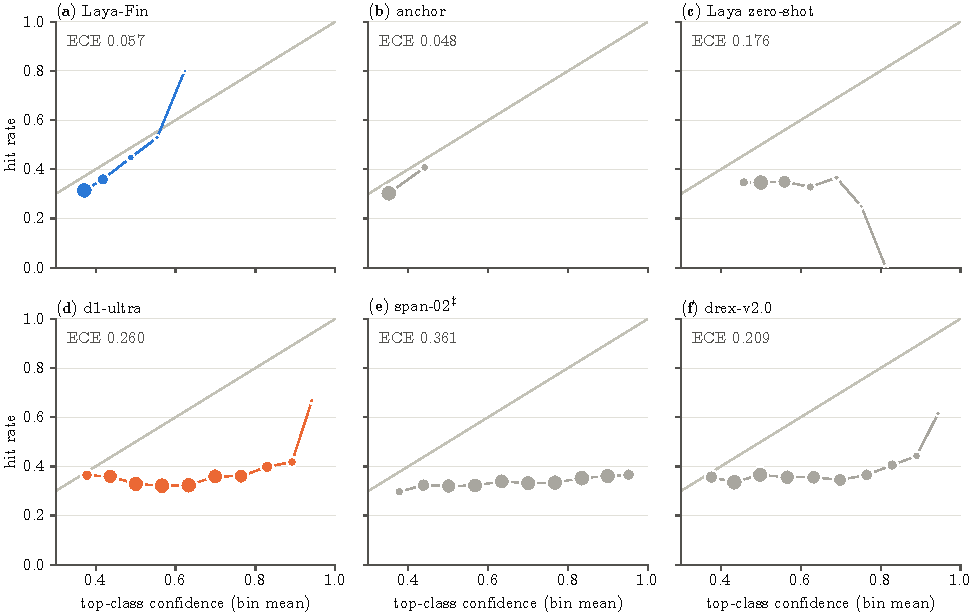
\includegraphics{figA4_reliability.pdf}
\caption{\textbf{Reliability of the three-class forecasts.} Reliability of Q1's three classes (fall, no move or rise at $\pm$0.5 typical moves) against $e_5$ on the test period: the hit rate of the top class by bin of its confidence (15 bins; dot area grows with the events in the bin; the diagonal is perfect calibration; NA-12). The trained models are calibrated but barely informative: ECE 0.057 for Laya-Fin and 0.048 for the anchor (uninformative, near-constant outputs), with log-loss skill 0.001 for Laya-Fin. The zero-shot and API models are overconfident: ECE 0.176 for Laya zero-shot, 0.260 for d1-ultra, 0.361 for span-02 and 0.209 for drex-v2.0. $\ddagger$ span-02: the S5 canary fired a STOP after the freeze and the operator chose to proceed (PREREG \S{}15).}\label{fig:figA4_reliability}
\end{figure}

\clearpage

\begin{figure}[htbp]
\centering
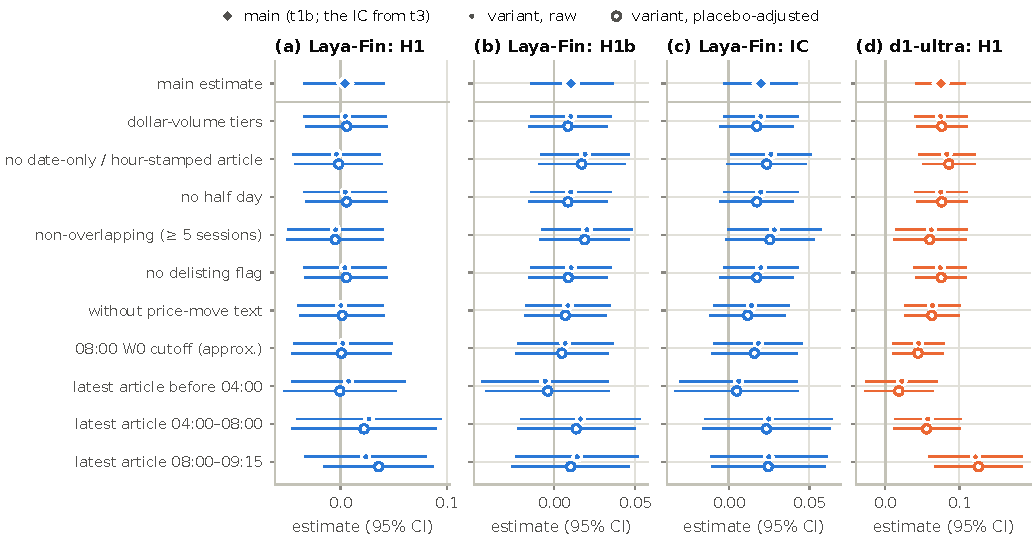
\includegraphics{figA5_robustness.pdf}
\caption{\textbf{No robustness variant changes a conclusion.} Robustness of the D0 results (\S{}11.6): Laya-Fin's H1, H1b and IC of $\hat N$ with $z_{cc}$, and d1-ultra's H1, in each variant raw (filled) and placebo-adjusted (hollow), below the main estimate (diamond; stationary block bootstrap) with 95\% intervals ($\pm$1.96 Newey--West SE for the variants). (a) and (d), both H1, share a scale; (b) and (c) have their own. Laya-Fin's H1 and H1b stay within their intervals of zero in every variant. d1-ultra's H1 stays positive in every variant, from 0.022 when the latest article precedes 04:00 to 0.122 when it falls between 08:00 and 09:15; it is model-specific (\S{}1.3).}\label{fig:figA5_robustness}
\end{figure}

\clearpage

\begin{figure}[htbp]
\centering
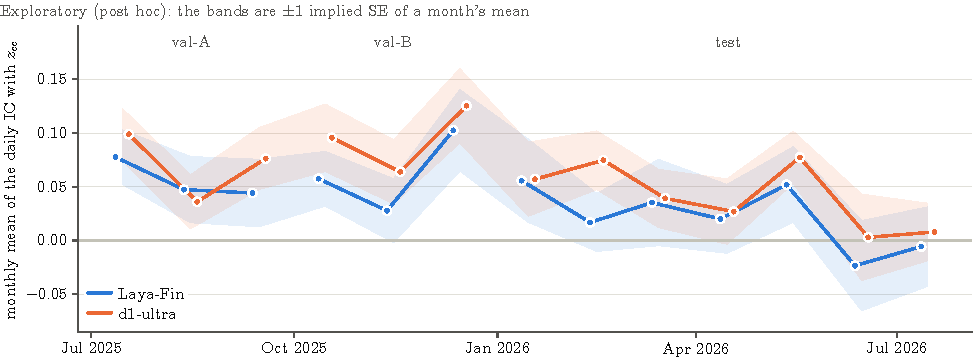
\includegraphics{figA6_monthly_ic.pdf}
\caption{\textbf{Exploratory: the monthly IC, with the implied standard error of a month's mean.} Exploratory (post hoc): the bands come from NA-12 \S{}13, requested after unblinding; no hypothesis, no claim. The monthly mean of the daily IC of $\hat N$ with $z_{cc}$ over val-A, val-B and the test period for Laya-Fin and d1-ultra (model-specific), with $\pm$1 implied standard error of a month's mean (iid; on test 0.037 for Laya-Fin). In the last two test months the ICs are about zero (Laya-Fin $-$0.02 and $-$0.01, d1-ultra +0.00 and +0.01), within about one standard error of a month's mean. Every release lies after the sample, where the time axis stops, which ends on 2026-07-31: Laya on 2026-09-18, the API models from 2026-10-12; a contamination cliff at a release would fall outside the data. The anchor (uninformative, near-constant outputs) has no implied SE; its monthly ICs are in the appendix's monthly table. $\ddagger$ span-02, whose release closes the API models' range: the S5 canary fired a STOP after the freeze and the operator chose to proceed (PREREG \S{}15).}\label{fig:figA6_monthly_ic}
\end{figure}

\clearpage

% t1b_primary_by_model: tab:a-primary-by-model (NA-14 figures.latex, from artifacts/NA-14/tables/t1b_primary_by_model.csv)
\begin{table}[htbp]
\centering
\small
\begin{threeparttable}
\caption{The primary tests for every model.}\label{tab:a-primary-by-model}
\begin{tabular}{@{}lS[table-format=-1.4]cS[table-format=-1.2]S[table-format=<1.3]S[table-format=<1.3]S[table-format=5.0]@{}}
\toprule
Test & {Estimate} & 95\% CI & {$t$} & {$p$} & {Holm $p$} & {Events} \\
\midrule
\multicolumn{7}{@{}l}{\textit{Laya-Fin}} \\
H1 & 0.0046 & [$-0.0346$, $0.0414$] & 0.23 & 0.409 & 0.853 & 13748 \\
H1b & 0.0105 & [$-0.0144$, $0.0366$] & 0.82 & 0.213 & 0.853 & 13748 \\
H2 & -0.0440 & --- & {---} & 0.616 & 0.853 & {---} \\
H3 & 0.0038 & [$-0.0008$, $0.0085$] & 1.52 & 0.054 & 0.269 & 17044 \\
H4 & 0.0012 & [$-0.0017$, $0.0042$] & {---} & 0.216 & 0.853 & 13732 \\
\addlinespace
\multicolumn{7}{@{}l}{\textit{anchor}} \\
H1 & 0.0036 & [$-0.0271$, $0.0342$] & 0.22 & 0.406 & 1.000 & 13748 \\
H1b & 0.0020 & [$-0.0192$, $0.0224$] & 0.18 & 0.427 & 1.000 & 13748 \\
H2 & 0.0150 & --- & {---} & 0.294 & 1.000 & {---} \\
H3 & 0.0013 & [$0.0002$, $0.0024$] & 2.10 & 0.017 & 0.083 & 17044 \\
H4 & -0.0004 & [$-0.0016$, $0.0007$] & {---} & 0.773 & 1.000 & 13732 \\
\addlinespace
\multicolumn{7}{@{}l}{\textit{Laya zero-shot}} \\
H1 & 0.0540 & [$0.0231$, $0.0867$] & 3.17 & 0.001 & 0.004 & 13748 \\
H1b & -0.0173 & [$-0.0438$, $0.0086$] & -1.25 & 0.900 & 1.000 & 13748 \\
H2 & {---} & --- & {---} & {---} & {---} & {---} \\
H3 & {---} & --- & {---} & {---} & {---} & {---} \\
H4 & -0.0013 & [$-0.0023$, $-0.0002$] & {---} & 0.992 & 1.000 & 13732 \\
\addlinespace
\multicolumn{7}{@{}l}{\textit{d1-ultra}} \\
H1 & 0.0748 & [$0.0405$, $0.1088$] & 4.13 & <0.001 & <0.001 & 13748 \\
H1b & -0.0007 & [$-0.0207$, $0.0198$] & -0.07 & 0.531 & 1.000 & 13748 \\
H2 & -0.0756 & --- & {---} & 0.991 & 1.000 & {---} \\
H3 & 0.0007 & [$-0.0017$, $0.0032$] & 0.52 & 0.285 & 1.000 & 17044 \\
H4 & 0.0004 & [$-0.0019$, $0.0028$] & {---} & 0.354 & 1.000 & 13732 \\
\addlinespace
\multicolumn{7}{@{}l}{\textit{span-02$^{\ddagger}$}} \\
H1 & 0.0748 & [$0.0389$, $0.1102$] & 4.05 & <0.001 & <0.001 & 13748 \\
H1b & -0.0005 & [$-0.0216$, $0.0205$] & -0.05 & 0.521 & 0.521 & 13748 \\
H2 & {---} & --- & {---} & {---} & {---} & {---} \\
H3 & {---} & --- & {---} & {---} & {---} & {---} \\
H4 & {---} & --- & {---} & {---} & {---} & {---} \\
\addlinespace
\multicolumn{7}{@{}l}{\textit{drex-v2.0}} \\
H1 & 0.0753 & [$0.0436$, $0.1062$] & 4.66 & <0.001 & <0.001 & 13748 \\
H1b & 0.0019 & [$-0.0178$, $0.0224$] & 0.18 & 0.426 & 0.426 & 13748 \\
H2 & {---} & --- & {---} & {---} & {---} & {---} \\
H3 & {---} & --- & {---} & {---} & {---} & {---} \\
H4 & {---} & --- & {---} & {---} & {---} & {---} \\
\bottomrule
\end{tabular}
\begin{tablenotes}[flushleft]\footnotesize
\item Holm within each model; the verdict is Laya-Fin's (Table~\ref{tab:primary}).
\item The anchor's readings are uninformative (near-constant outputs after one epoch); its rows are reported, not read as nulls.
\item The API models fail the \S8.3 contamination screens, so their results are model-specific (\S1.3).
\item $^{\ddagger}$span-02: the S5 canary fired a STOP after the freeze; the operator chose to proceed (PREREG \S15, post-freeze NA-11 row).
\end{tablenotes}
\end{threeparttable}
\end{table}


\clearpage

% t3_ic (NA-14, from artifacts/NA-12/tables/t3_ic.csv)
\begin{table*}[tbp]
\centering\small
\caption{Daily IC of \^{N}\_W0 with z\_cc, z\_on and z\_id, and quintile spreads (\S{}11.1)}\label{tab:t3_ic}
\begin{adjustbox}{max width=\textwidth}
\begin{tabular}{llrrrrrrrrr}
\toprule
model & target & IC & IC t & IC CI low & IC CI high & n days & n obs & qspread & qspread t & qspread p \\
\midrule
Laya-Fin & z\_cc & $0.020$ & $1.671$ & $-0.003$ & $0.042$ & $140$ & $13{,}748$ & $0.127$ & $1.918$ & $0.024$ \\
Laya-Fin & z\_on & $0.015$ & $1.079$ & $-0.011$ & $0.041$ & $138$ & $13{,}439$ & $0.174$ & $1.679$ & $0.044$ \\
Laya-Fin & z\_id & $0.010$ & $0.815$ & $-0.015$ & $0.036$ & $138$ & $13{,}439$ & $0.050$ & $0.845$ & $0.201$ \\
anchor (uninformative) & z\_cc & $0.008$ & $0.826$ & $-0.011$ & $0.026$ & $140$ & $13{,}748$ & $-0.001$ & $-0.017$ & $0.500$ \\
anchor (uninformative) & z\_on & $0.006$ & $0.498$ & $-0.016$ & $0.027$ & $138$ & $13{,}439$ & $-0.011$ & $-0.105$ & $0.544$ \\
anchor (uninformative) & z\_id & $0.002$ & $0.181$ & $-0.020$ & $0.022$ & $138$ & $13{,}439$ & $0.002$ & $0.033$ & $0.495$ \\
Laya zero-shot & z\_cc & $0.005$ & $0.369$ & $-0.023$ & $0.032$ & $140$ & $13{,}748$ & $0.056$ & $0.712$ & $0.236$ \\
Laya zero-shot & z\_on & $0.037$ & $3.222$ & $0.015$ & $0.058$ & $138$ & $13{,}439$ & $0.281$ & $3.334$ & $<0.001$ \\
Laya zero-shot & z\_id & $-0.017$ & $-1.251$ & $-0.043$ & $0.008$ & $138$ & $13{,}439$ & $-0.102$ & $-1.561$ & $0.953$ \\
d1-ultra & z\_cc & $0.039$ & $3.229$ & $0.015$ & $0.062$ & $140$ & $13{,}748$ & $0.410$ & $5.091$ & $<0.001$ \\
d1-ultra & z\_on & $0.074$ & $4.739$ & $0.043$ & $0.104$ & $138$ & $13{,}439$ & $0.812$ & $5.602$ & $<0.001$ \\
d1-ultra & z\_id & $-7.37\times 10^{-4}$ & $-0.068$ & $-0.021$ & $0.020$ & $138$ & $13{,}439$ & $-0.006$ & $-0.127$ & $0.547$ \\
span-02\textsuperscript{\ddag} & z\_cc & $0.041$ & $3.098$ & $0.015$ & $0.064$ & $140$ & $13{,}748$ & $0.406$ & $4.969$ & $<0.001$ \\
span-02\textsuperscript{\ddag} & z\_on & $0.074$ & $4.487$ & $0.040$ & $0.106$ & $138$ & $13{,}439$ & $0.803$ & $6.003$ & $<0.001$ \\
span-02\textsuperscript{\ddag} & z\_id & $-5.40\times 10^{-4}$ & $-0.048$ & $-0.021$ & $0.020$ & $138$ & $13{,}439$ & $-0.008$ & $-0.163$ & $0.566$ \\
drex-v2.0 & z\_cc & $0.044$ & $3.696$ & $0.021$ & $0.067$ & $140$ & $13{,}748$ & $0.384$ & $5.032$ & $<0.001$ \\
drex-v2.0 & z\_on & $0.077$ & $5.340$ & $0.048$ & $0.105$ & $138$ & $13{,}439$ & $0.760$ & $6.216$ & $<0.001$ \\
drex-v2.0 & z\_id & $0.002$ & $0.176$ & $-0.018$ & $0.023$ & $138$ & $13{,}439$ & $-0.005$ & $-0.103$ & $0.541$ \\
\bottomrule
\end{tabular}
\end{adjustbox}
\par\smallskip{\footnotesize\raggedright The anchor's readings are uninformative (near-constant outputs: NA-11 REPORT \S{}7.1 item 4); its rows are reported, not read as nulls. \textsuperscript{\ddag} span-02: the S5 canary fired a STOP after the freeze; the operator chose to proceed (PREREG \S{}15, the post-freeze NA-11 S5 row).\par}
\end{table*}


\clearpage

% t32_val_b_ic: tab:a-val-b-ic (NA-14 figures.latex, from artifacts/NA-14/tables/t32_val_b_ic.csv)
\begin{table}[htbp]
\centering
\small
\begin{threeparttable}
\caption{Val-B daily ICs by target of the trained and zero-shot Laya models (NA-11, before the freeze).}\label{tab:a-val-b-ic}
\begin{tabular}{@{}lS[table-format=-1.3]S[table-format=-1.2]S[table-format=-1.3]S[table-format=-1.2]S[table-format=-1.3]S[table-format=-1.2]S[table-format=4.0]@{}}
\toprule
Model & {IC $z_{cc}$} & {$t$} & {IC $z_{on}$} & {$t$} & {IC $z_{id}$} & {$t$} & {Events} \\
\midrule
Laya-Fin & 0.065 & 3.64 & 0.045 & 2.93 & 0.054 & 2.89 & 5506 \\
anchor & -0.020 & -1.52 & -0.002 & -0.16 & -0.011 & -0.75 & 5506 \\
Laya zero-shot & 0.029 & 1.94 & 0.047 & 2.55 & 0.002 & 0.12 & 5506 \\
\bottomrule
\end{tabular}
\begin{tablenotes}[flushleft]\footnotesize
\item From NA-11's run of the frozen spec on val-B, before the freeze.
\item The anchor's readings are uninformative (near-constant outputs after one epoch); its rows are reported, not read as nulls.
\end{tablenotes}
\end{threeparttable}
\end{table}


\clearpage

% t15_calibration (NA-14, from artifacts/NA-12/tables/t15_calibration.csv)
\begin{table*}[tbp]
\centering\small
\caption{\S{}11.2 calibration of Q1's three classes (ECE; log-loss and Brier skill vs val-A climatology); H7}\label{tab:t15_calibration}
\begin{adjustbox}{max width=\textwidth}
\begin{tabular}{llrrrrrrrrrr>{\raggedright\arraybackslash}p{12em}}
\toprule
model & target & ECE & log loss & brier & log loss skill & brier skill & n & AUC & temperature & ECE before & ECE after & source \\
\midrule
Laya-Fin & e5 & $0.057$ & $1.097$ & $0.667$ & $7.51\times 10^{-4}$ & $-3.32\times 10^{-4}$ & $13{,}139$ & --- & --- & --- & --- & --- \\
Laya-Fin & z\_cc & $0.033$ & $1.093$ & $0.664$ & $0.010$ & $0.010$ & $13{,}748$ & --- & --- & --- & --- & --- \\
Laya-Fin & $|$z\_cc$|$ $>$= 1 & --- & --- & --- & --- & --- & --- & $0.603$ & --- & --- & --- & --- \\
Laya-Fin & e5 & --- & --- & --- & --- & --- & --- & --- & $1.002$ & $0.058$ & $0.057$ & NA-08 val-A temperature (the files' probabilities) vs T = 1 on the logits \\
anchor (uninformative) & e5 & $0.048$ & $1.096$ & $0.666$ & $0.002$ & $0.001$ & $13{,}139$ & --- & --- & --- & --- & --- \\
anchor (uninformative) & z\_cc & $0.016$ & $1.087$ & $0.660$ & $0.015$ & $0.015$ & $13{,}748$ & --- & --- & --- & --- & --- \\
anchor (uninformative) & $|$z\_cc$|$ $>$= 1 & --- & --- & --- & --- & --- & --- & $0.576$ & --- & --- & --- & --- \\
anchor (uninformative) & e5 & --- & --- & --- & --- & --- & --- & --- & $0.966$ & $0.011$ & $0.048$ & NA-08 val-A temperature (the files' probabilities) vs T = 1 on the logits \\
Laya zero-shot & e5 & $0.176$ & $1.270$ & $0.739$ & $-0.156$ & $-0.110$ & $13{,}139$ & --- & --- & --- & --- & --- \\
Laya zero-shot & z\_cc & $0.179$ & $1.300$ & $0.751$ & $-0.177$ & $-0.120$ & $13{,}748$ & --- & --- & --- & --- & --- \\
Laya zero-shot & $|$z\_cc$|$ $>$= 1 & --- & --- & --- & --- & --- & --- & $0.523$ & --- & --- & --- & --- \\
Laya zero-shot & e5 & --- & --- & --- & --- & --- & --- & --- & $6.329$ & $0.176$ & $0.110$ & one Q1 temperature fit on val-A (NA-08's rule), applied to the evaluation split \\
d1-ultra & e5 & $0.260$ & $1.311$ & $0.796$ & $-0.194$ & $-0.194$ & $13{,}139$ & --- & --- & --- & --- & --- \\
d1-ultra & z\_cc & $0.249$ & $1.287$ & $0.781$ & $-0.166$ & $-0.165$ & $13{,}748$ & --- & --- & --- & --- & --- \\
d1-ultra & $|$z\_cc$|$ $>$= 1 & --- & --- & --- & --- & --- & --- & $0.580$ & --- & --- & --- & --- \\
d1-ultra & e5 & --- & --- & --- & --- & --- & --- & --- & $1.945$ & $0.260$ & $0.155$ & one Q1 temperature fit on val-A (NA-08's rule), applied to the evaluation split \\
span-02\textsuperscript{\ddag} & e5 & $0.361$ & $1.603$ & $0.907$ & $-0.460$ & $-0.361$ & $13{,}139$ & --- & --- & --- & --- & --- \\
span-02\textsuperscript{\ddag} & z\_cc & $0.342$ & $1.556$ & $0.881$ & $-0.410$ & $-0.315$ & $13{,}748$ & --- & --- & --- & --- & --- \\
span-02\textsuperscript{\ddag} & $|$z\_cc$|$ $>$= 1 & --- & --- & --- & --- & --- & --- & $0.556$ & --- & --- & --- & --- \\
drex-v2.0 & e5 & $0.209$ & $1.247$ & $0.758$ & $-0.135$ & $-0.138$ & $13{,}139$ & --- & --- & --- & --- & --- \\
drex-v2.0 & z\_cc & $0.204$ & $1.235$ & $0.751$ & $-0.119$ & $-0.120$ & $13{,}748$ & --- & --- & --- & --- & --- \\
drex-v2.0 & $|$z\_cc$|$ $>$= 1 & --- & --- & --- & --- & --- & --- & $0.566$ & --- & --- & --- & --- \\
\bottomrule
\end{tabular}
\end{adjustbox}
\par\smallskip{\footnotesize\raggedright The anchor's readings are uninformative (near-constant outputs: NA-11 REPORT \S{}7.1 item 4); its rows are reported, not read as nulls. \textsuperscript{\ddag} span-02: the S5 canary fired a STOP after the freeze; the operator chose to proceed (PREREG \S{}15, the post-freeze NA-11 S5 row).\par}
\end{table*}


\clearpage

% t16_robustness: tab:a-robustness (NA-14 figures.latex, from artifacts/NA-14/tables/t16_robustness.csv)
\begin{landscape}
\begingroup
\footnotesize
\setlength{\tabcolsep}{4pt}
\begin{longtable}{@{}lS[table-format=-1.3]S[table-format=1.3, table-space-text-pre={$<$}]S[table-format=-1.3]S[table-format=1.3]S[table-format=-1.3]S[table-format=-1.3]S[table-format=1.3]S[table-format=-1.3]S[table-format=1.3]S[table-format=-1.3]@{}}
\caption{Robustness of the primary results: no variant changes a conclusion.}\label{tab:a-robustness} \\
\toprule
Model, point, variant & {H1} & {$p$} & {H1b} & {$p$} & {IC $z_{cc}$} & {$b$} & {$p_b$} & {$c$} & {$p_c$} & {IC $y_2$} \\
\midrule
\endfirsthead
\multicolumn{11}{@{}l}{\textit{Table \ref{tab:a-robustness}, continued}} \\
\toprule
Model, point, variant & {H1} & {$p$} & {H1b} & {$p$} & {IC $z_{cc}$} & {$b$} & {$p_b$} & {$c$} & {$p_c$} & {IC $y_2$} \\
\midrule
\endhead
\midrule
\multicolumn{11}{r@{}}{\textit{continued on the next page}} \\
\endfoot
\bottomrule
\endlastfoot
Laya-Fin, D0, dollar-volume tiers, raw & 0.005 & 0.409 & 0.010 & 0.213 & 0.020 & {---} & {---} & {---} & {---} & {---} \\
Laya-Fin, D0, no date-only or hour-stamped article, raw & -0.004 & 0.577 & 0.019 & 0.091 & 0.026 & {---} & {---} & {---} & {---} & {---} \\
Laya-Fin, D0, no half days, raw & 0.005 & 0.409 & 0.010 & 0.213 & 0.020 & {---} & {---} & {---} & {---} & {---} \\
Laya-Fin, D0, non-overlapping events, raw & -0.005 & 0.567 & 0.020 & 0.084 & 0.028 & {---} & {---} & {---} & {---} & {---} \\
Laya-Fin, D0, no delisting flag, raw & 0.004 & 0.418 & 0.011 & 0.209 & 0.020 & {---} & {---} & {---} & {---} & {---} \\
Laya-Fin, D0, without price-move text, raw & 0.000 & 0.494 & 0.009 & 0.262 & 0.014 & {---} & {---} & {---} & {---} & {---} \\
Laya-Fin, D0, 08:00 cutoff (approximated), raw & 0.002 & 0.461 & 0.007 & 0.315 & 0.018 & {---} & {---} & {---} & {---} & {---} \\
Laya-Fin, D0, latest article 04:00 to 08:00, raw & 0.027 & 0.199 & 0.016 & 0.185 & 0.025 & {---} & {---} & {---} & {---} & {---} \\
Laya-Fin, D0, latest article 08:00 to 09:15, raw & 0.024 & 0.204 & 0.014 & 0.232 & 0.025 & {---} & {---} & {---} & {---} & {---} \\
Laya-Fin, D0, latest article before 04:00, raw & 0.008 & 0.402 & -0.005 & 0.591 & 0.006 & {---} & {---} & {---} & {---} & {---} \\
Laya-Fin, D2, dollar-volume tiers, raw & {---} & {---} & {---} & {---} & {---} & -0.038 & 0.601 & -0.014 & 0.114 & {---} \\
Laya-Fin, D2, no date-only or hour-stamped article, raw & {---} & {---} & {---} & {---} & {---} & -0.011 & 0.528 & -0.018 & 0.074 & {---} \\
Laya-Fin, D2, no half days, raw & {---} & {---} & {---} & {---} & {---} & -0.044 & 0.616 & -0.015 & 0.110 & {---} \\
Laya-Fin, D2, non-overlapping events, raw & {---} & {---} & {---} & {---} & {---} & -0.012 & 0.526 & 0.005 & 0.639 & {---} \\
Laya-Fin, D2, no delisting flag, raw & {---} & {---} & {---} & {---} & {---} & -0.050 & 0.630 & -0.015 & 0.114 & {---} \\
Laya-Fin, D0, dollar-volume tiers, placebo-adjusted & 0.006 & 0.384 & 0.009 & 0.249 & 0.017 & {---} & {---} & {---} & {---} & {---} \\
Laya-Fin, D0, no date-only or hour-stamped article, placebo-adjusted & -0.002 & 0.538 & 0.017 & 0.120 & 0.024 & {---} & {---} & {---} & {---} & {---} \\
Laya-Fin, D0, no half days, placebo-adjusted & 0.006 & 0.384 & 0.009 & 0.249 & 0.017 & {---} & {---} & {---} & {---} & {---} \\
Laya-Fin, D0, non-overlapping events, placebo-adjusted & -0.005 & 0.573 & 0.019 & 0.096 & 0.026 & {---} & {---} & {---} & {---} & {---} \\
Laya-Fin, D0, no delisting flag, placebo-adjusted & 0.006 & 0.391 & 0.009 & 0.245 & 0.017 & {---} & {---} & {---} & {---} & {---} \\
Laya-Fin, D0, without price-move text, placebo-adjusted & 0.002 & 0.473 & 0.007 & 0.294 & 0.012 & {---} & {---} & {---} & {---} & {---} \\
Laya-Fin, D0, 08:00 cutoff (approximated), placebo-adjusted & 0.001 & 0.486 & 0.005 & 0.361 & 0.016 & {---} & {---} & {---} & {---} & {---} \\
Laya-Fin, D0, latest article 04:00 to 08:00, placebo-adjusted & 0.022 & 0.245 & 0.014 & 0.225 & 0.023 & {---} & {---} & {---} & {---} & {---} \\
Laya-Fin, D0, latest article 08:00 to 09:15, placebo-adjusted & 0.036 & 0.088 & 0.010 & 0.295 & 0.024 & {---} & {---} & {---} & {---} & {---} \\
Laya-Fin, D0, latest article before 04:00, placebo-adjusted & 0.000 & 0.523 & -0.004 & 0.565 & 0.005 & {---} & {---} & {---} & {---} & {---} \\
Laya-Fin, D2, dollar-volume tiers, placebo-adjusted & {---} & {---} & {---} & {---} & {---} & -0.036 & 0.597 & -0.014 & 0.122 & {---} \\
Laya-Fin, D2, no date-only or hour-stamped article, placebo-adjusted & {---} & {---} & {---} & {---} & {---} & -0.011 & 0.528 & -0.018 & 0.074 & {---} \\
Laya-Fin, D2, no half days, placebo-adjusted & {---} & {---} & {---} & {---} & {---} & -0.044 & 0.616 & -0.015 & 0.110 & {---} \\
Laya-Fin, D2, non-overlapping events, placebo-adjusted & {---} & {---} & {---} & {---} & {---} & -0.012 & 0.526 & 0.005 & 0.639 & {---} \\
Laya-Fin, D2, no delisting flag, placebo-adjusted & {---} & {---} & {---} & {---} & {---} & -0.050 & 0.630 & -0.015 & 0.114 & {---} \\
Laya-Fin, D0+D2, placebo-adjusted & 0.006 & 0.384 & 0.009 & 0.249 & {---} & -0.044 & 0.616 & -0.015 & 0.110 & {---} \\
Laya-Fin, D0+D2, $\sigma$ = 60-session SD, raw & 0.007 & 0.367 & 0.009 & 0.238 & {---} & -0.032 & 0.607 & -0.013 & 0.109 & {---} \\
Laya-Fin, D0, 2024-H1, raw & 0.028 & 0.235 & 0.024 & 0.105 & 0.041 & {---} & {---} & {---} & {---} & {---} \\
Laya-Fin, D0, 2024-H1, placebo-adjusted & 0.022 & 0.291 & 0.025 & 0.103 & {---} & {---} & {---} & {---} & {---} & {---} \\
Laya-Fin, D2, 2024-H1, raw & {---} & {---} & {---} & {---} & {---} & 0.079 & 0.344 & 0.004 & 0.607 & {---} \\
Laya-Fin, D2, 2024-H1, placebo-adjusted & {---} & {---} & {---} & {---} & {---} & 0.079 & 0.344 & 0.004 & 0.607 & {---} \\
anchor, D0, dollar-volume tiers, raw & 0.004 & 0.406 & 0.002 & 0.427 & 0.008 & {---} & {---} & {---} & {---} & {---} \\
anchor, D0, no date-only or hour-stamped article, raw & 0.002 & 0.467 & 0.012 & 0.143 & 0.021 & {---} & {---} & {---} & {---} & {---} \\
anchor, D0, no half days, raw & 0.004 & 0.406 & 0.002 & 0.427 & 0.008 & {---} & {---} & {---} & {---} & {---} \\
anchor, D0, non-overlapping events, raw & -0.005 & 0.593 & 0.004 & 0.393 & 0.008 & {---} & {---} & {---} & {---} & {---} \\
anchor, D0, no delisting flag, raw & 0.004 & 0.404 & 0.002 & 0.426 & 0.008 & {---} & {---} & {---} & {---} & {---} \\
anchor, D0, without price-move text, raw & 0.008 & 0.294 & -0.006 & 0.700 & -0.002 & {---} & {---} & {---} & {---} & {---} \\
anchor, D0, 08:00 cutoff (approximated), raw & -0.008 & 0.710 & 0.006 & 0.300 & 0.002 & {---} & {---} & {---} & {---} & {---} \\
anchor, D0, latest article 04:00 to 08:00, raw & -0.030 & 0.840 & 0.041 & 0.023 & 0.034 & {---} & {---} & {---} & {---} & {---} \\
anchor, D0, latest article 08:00 to 09:15, raw & 0.047 & 0.070 & -0.008 & 0.634 & 0.025 & {---} & {---} & {---} & {---} & {---} \\
anchor, D0, latest article before 04:00, raw & -0.013 & 0.751 & 0.001 & 0.487 & -0.006 & {---} & {---} & {---} & {---} & {---} \\
anchor, D2, dollar-volume tiers, raw & {---} & {---} & {---} & {---} & {---} & 0.775 & 0.292 & -0.015 & 0.116 & {---} \\
anchor, D2, no date-only or hour-stamped article, raw & {---} & {---} & {---} & {---} & {---} & 0.306 & 0.408 & -0.018 & 0.076 & {---} \\
anchor, D2, no half days, raw & {---} & {---} & {---} & {---} & {---} & 0.748 & 0.294 & -0.015 & 0.111 & {---} \\
anchor, D2, non-overlapping events, raw & {---} & {---} & {---} & {---} & {---} & 3.898 & 0.034 & 0.006 & 0.655 & {---} \\
anchor, D2, no delisting flag, raw & {---} & {---} & {---} & {---} & {---} & 0.752 & 0.293 & -0.015 & 0.114 & {---} \\
anchor, D0, dollar-volume tiers, placebo-adjusted & 0.006 & 0.345 & 0.002 & 0.429 & 0.008 & {---} & {---} & {---} & {---} & {---} \\
anchor, D0, no date-only or hour-stamped article, placebo-adjusted & 0.003 & 0.427 & 0.013 & 0.128 & 0.022 & {---} & {---} & {---} & {---} & {---} \\
anchor, D0, no half days, placebo-adjusted & 0.006 & 0.345 & 0.002 & 0.429 & 0.008 & {---} & {---} & {---} & {---} & {---} \\
anchor, D0, non-overlapping events, placebo-adjusted & -0.002 & 0.533 & 0.004 & 0.395 & 0.007 & {---} & {---} & {---} & {---} & {---} \\
anchor, D0, no delisting flag, placebo-adjusted & 0.006 & 0.351 & 0.002 & 0.423 & 0.008 & {---} & {---} & {---} & {---} & {---} \\
anchor, D0, without price-move text, placebo-adjusted & 0.009 & 0.262 & -0.006 & 0.701 & -0.003 & {---} & {---} & {---} & {---} & {---} \\
anchor, D0, 08:00 cutoff (approximated), placebo-adjusted & -0.005 & 0.627 & 0.005 & 0.323 & 0.002 & {---} & {---} & {---} & {---} & {---} \\
anchor, D0, latest article 04:00 to 08:00, placebo-adjusted & -0.027 & 0.814 & 0.040 & 0.025 & 0.030 & {---} & {---} & {---} & {---} & {---} \\
anchor, D0, latest article 08:00 to 09:15, placebo-adjusted & 0.044 & 0.074 & -0.005 & 0.585 & 0.022 & {---} & {---} & {---} & {---} & {---} \\
anchor, D0, latest article before 04:00, placebo-adjusted & -0.009 & 0.689 & 0.000 & 0.501 & -0.005 & {---} & {---} & {---} & {---} & {---} \\
anchor, D2, dollar-volume tiers, placebo-adjusted & {---} & {---} & {---} & {---} & {---} & 0.693 & 0.308 & -0.014 & 0.124 & {---} \\
anchor, D2, no date-only or hour-stamped article, placebo-adjusted & {---} & {---} & {---} & {---} & {---} & 0.306 & 0.408 & -0.018 & 0.076 & {---} \\
anchor, D2, no half days, placebo-adjusted & {---} & {---} & {---} & {---} & {---} & 0.748 & 0.294 & -0.015 & 0.111 & {---} \\
anchor, D2, non-overlapping events, placebo-adjusted & {---} & {---} & {---} & {---} & {---} & 3.898 & 0.034 & 0.006 & 0.655 & {---} \\
anchor, D2, no delisting flag, placebo-adjusted & {---} & {---} & {---} & {---} & {---} & 0.752 & 0.293 & -0.015 & 0.114 & {---} \\
anchor, D0+D2, placebo-adjusted & 0.006 & 0.345 & 0.002 & 0.429 & {---} & 0.748 & 0.294 & -0.015 & 0.111 & {---} \\
anchor, D0+D2, $\sigma$ = 60-session SD, raw & 0.005 & 0.372 & -0.001 & 0.528 & {---} & 0.673 & 0.254 & -0.013 & 0.110 & {---} \\
anchor, D0, 2024-H1, raw & -0.043 & 0.895 & 0.026 & 0.127 & 0.011 & {---} & {---} & {---} & {---} & {---} \\
anchor, D0, 2024-H1, placebo-adjusted & -0.042 & 0.889 & 0.024 & 0.151 & {---} & {---} & {---} & {---} & {---} & {---} \\
anchor, D2, 2024-H1, raw & {---} & {---} & {---} & {---} & {---} & 1.845 & 0.156 & 0.004 & 0.613 & {---} \\
anchor, D2, 2024-H1, placebo-adjusted & {---} & {---} & {---} & {---} & {---} & 1.845 & 0.156 & 0.004 & 0.613 & {---} \\
d1-ultra, D0, dollar-volume tiers, raw & 0.075 & {$<$}0.001 & -0.001 & 0.531 & 0.039 & {---} & {---} & {---} & {---} & {---} \\
d1-ultra, D0, no date-only or hour-stamped article, raw & 0.083 & {$<$}0.001 & -0.001 & 0.542 & 0.042 & {---} & {---} & {---} & {---} & {---} \\
d1-ultra, D0, no half days, raw & 0.075 & {$<$}0.001 & -0.001 & 0.531 & 0.039 & {---} & {---} & {---} & {---} & {---} \\
d1-ultra, D0, non-overlapping events, raw & 0.062 & 0.005 & 0.015 & 0.141 & 0.060 & {---} & {---} & {---} & {---} & {---} \\
d1-ultra, D0, no delisting flag, raw & 0.074 & {$<$}0.001 & 0.000 & 0.522 & 0.039 & {---} & {---} & {---} & {---} & {---} \\
d1-ultra, D0, without price-move text, raw & 0.064 & {$<$}0.001 & 0.001 & 0.462 & 0.036 & {---} & {---} & {---} & {---} & {---} \\
d1-ultra, D0, 08:00 cutoff (approximated), raw & 0.045 & 0.003 & 0.000 & 0.509 & 0.023 & {---} & {---} & {---} & {---} & {---} \\
d1-ultra, D0, latest article 04:00 to 08:00, raw & 0.057 & 0.004 & 0.004 & 0.438 & 0.030 & {---} & {---} & {---} & {---} & {---} \\
d1-ultra, D0, latest article 08:00 to 09:15, raw & 0.122 & {$<$}0.001 & -0.006 & 0.621 & 0.057 & {---} & {---} & {---} & {---} & {---} \\
d1-ultra, D0, latest article before 04:00, raw & 0.022 & 0.170 & 0.001 & 0.465 & 0.019 & {---} & {---} & {---} & {---} & {---} \\
d1-ultra, D2, dollar-volume tiers, raw & {---} & {---} & {---} & {---} & {---} & -0.074 & 0.990 & -0.011 & 0.177 & {---} \\
d1-ultra, D2, no date-only or hour-stamped article, raw & {---} & {---} & {---} & {---} & {---} & -0.074 & 0.984 & -0.014 & 0.123 & {---} \\
d1-ultra, D2, no half days, raw & {---} & {---} & {---} & {---} & {---} & -0.076 & 0.991 & -0.011 & 0.171 & {---} \\
d1-ultra, D2, non-overlapping events, raw & {---} & {---} & {---} & {---} & {---} & -0.062 & 0.950 & 0.008 & 0.711 & {---} \\
d1-ultra, D2, no delisting flag, raw & {---} & {---} & {---} & {---} & {---} & -0.076 & 0.991 & -0.011 & 0.176 & {---} \\
d1-ultra, D0, dollar-volume tiers, placebo-adjusted & 0.076 & {$<$}0.001 & -0.002 & 0.586 & 0.038 & {---} & {---} & {---} & {---} & {---} \\
d1-ultra, D0, no date-only or hour-stamped article, placebo-adjusted & 0.086 & {$<$}0.001 & -0.004 & 0.636 & 0.041 & {---} & {---} & {---} & {---} & {---} \\
d1-ultra, D0, no half days, placebo-adjusted & 0.076 & {$<$}0.001 & -0.002 & 0.586 & 0.038 & {---} & {---} & {---} & {---} & {---} \\
d1-ultra, D0, non-overlapping events, placebo-adjusted & 0.060 & 0.007 & 0.016 & 0.137 & 0.064 & {---} & {---} & {---} & {---} & {---} \\
d1-ultra, D0, no delisting flag, placebo-adjusted & 0.075 & {$<$}0.001 & -0.002 & 0.572 & 0.038 & {---} & {---} & {---} & {---} & {---} \\
d1-ultra, D0, without price-move text, placebo-adjusted & 0.063 & {$<$}0.001 & 0.002 & 0.459 & 0.036 & {---} & {---} & {---} & {---} & {---} \\
d1-ultra, D0, 08:00 cutoff (approximated), placebo-adjusted & 0.044 & 0.003 & 0.001 & 0.474 & 0.027 & {---} & {---} & {---} & {---} & {---} \\
d1-ultra, D0, latest article 04:00 to 08:00, placebo-adjusted & 0.056 & 0.005 & 0.004 & 0.435 & 0.029 & {---} & {---} & {---} & {---} & {---} \\
d1-ultra, D0, latest article 08:00 to 09:15, placebo-adjusted & 0.126 & {$<$}0.001 & -0.006 & 0.630 & 0.050 & {---} & {---} & {---} & {---} & {---} \\
d1-ultra, D0, latest article before 04:00, placebo-adjusted & 0.018 & 0.212 & 0.005 & 0.372 & 0.024 & {---} & {---} & {---} & {---} & {---} \\
d1-ultra, D2, dollar-volume tiers, placebo-adjusted & {---} & {---} & {---} & {---} & {---} & -0.075 & 0.991 & -0.011 & 0.189 & {---} \\
d1-ultra, D2, no date-only or hour-stamped article, placebo-adjusted & {---} & {---} & {---} & {---} & {---} & -0.074 & 0.984 & -0.014 & 0.123 & {---} \\
d1-ultra, D2, no half days, placebo-adjusted & {---} & {---} & {---} & {---} & {---} & -0.076 & 0.991 & -0.011 & 0.171 & {---} \\
d1-ultra, D2, non-overlapping events, placebo-adjusted & {---} & {---} & {---} & {---} & {---} & -0.062 & 0.950 & 0.008 & 0.711 & {---} \\
d1-ultra, D2, no delisting flag, placebo-adjusted & {---} & {---} & {---} & {---} & {---} & -0.076 & 0.991 & -0.011 & 0.176 & {---} \\
d1-ultra, D0+D2, placebo-adjusted & 0.076 & {$<$}0.001 & -0.002 & 0.586 & {---} & -0.076 & 0.991 & -0.011 & 0.171 & {---} \\
d1-ultra, D0+D2, $\sigma$ = 60-session SD, raw & 0.075 & {$<$}0.001 & -0.001 & 0.555 & {---} & -0.056 & 0.991 & -0.009 & 0.179 & {---} \\
d1-ultra, D0, 2024-H1, raw & 0.153 & 0.001 & 0.020 & 0.255 & 0.109 & {---} & {---} & {---} & {---} & {---} \\
d1-ultra, D0, 2024-H1, placebo-adjusted & 0.146 & {$<$}0.001 & 0.021 & 0.234 & {---} & {---} & {---} & {---} & {---} & {---} \\
d1-ultra, D2, 2024-H1, raw & {---} & {---} & {---} & {---} & {---} & 0.015 & 0.382 & 0.004 & 0.601 & {---} \\
d1-ultra, D2, 2024-H1, placebo-adjusted & {---} & {---} & {---} & {---} & {---} & 0.015 & 0.382 & 0.004 & 0.601 & {---} \\
d1-ultra, D0, unmasked twins: masked reading, raw & 0.063 & 0.003 & -0.009 & 0.736 & 0.026 & {---} & {---} & {---} & {---} & {---} \\
d1-ultra, D0, unmasked twins: unmasked reading, raw & 0.074 & {$<$}0.001 & -0.009 & 0.735 & 0.029 & {---} & {---} & {---} & {---} & {---} \\
d1-ultra, D2, Call B, news removed: $J$ (real), raw & {---} & {---} & {---} & {---} & {---} & {---} & {---} & {---} & {---} & -0.020 \\
d1-ultra, D2, Call B, news removed: $J$ (ablated), raw & {---} & {---} & {---} & {---} & {---} & {---} & {---} & {---} & {---} & -0.012 \\
d1-ultra, D2, Call B, news removed: $C$ (real), raw & {---} & {---} & {---} & {---} & {---} & {---} & {---} & {---} & {---} & -0.019 \\
d1-ultra, D2, Call B, news removed: $C$ (ablated), raw & {---} & {---} & {---} & {---} & {---} & {---} & {---} & {---} & {---} & -0.014 \\
d1-ultra, D2, Call B, news removed: $\hat N$ (real), raw & {---} & {---} & {---} & {---} & {---} & {---} & {---} & {---} & {---} & -0.015 \\
d1-ultra, D2, Call B, news removed: $\hat N$ (ablated), raw & {---} & {---} & {---} & {---} & {---} & {---} & {---} & {---} & {---} & 0.018 \\
d1-ultra, D2, Call B, shuffled news: $J$ (real), raw & {---} & {---} & {---} & {---} & {---} & {---} & {---} & {---} & {---} & -0.021 \\
d1-ultra, D2, Call B, shuffled news: $J$ (ablated), raw & {---} & {---} & {---} & {---} & {---} & {---} & {---} & {---} & {---} & -0.001 \\
d1-ultra, D2, Call B, shuffled news: $C$ (real), raw & {---} & {---} & {---} & {---} & {---} & {---} & {---} & {---} & {---} & -0.022 \\
d1-ultra, D2, Call B, shuffled news: $C$ (ablated), raw & {---} & {---} & {---} & {---} & {---} & {---} & {---} & {---} & {---} & -0.005 \\
d1-ultra, D2, Call B, shuffled news: $\hat N$ (real), raw & {---} & {---} & {---} & {---} & {---} & {---} & {---} & {---} & {---} & -0.013 \\
d1-ultra, D2, Call B, shuffled news: $\hat N$ (ablated), raw & {---} & {---} & {---} & {---} & {---} & {---} & {---} & {---} & {---} & 0.008 \\
all tiers, summary text, not run & {---} & {---} & {---} & {---} & {---} & {---} & {---} & {---} & {---} & {---} \\
all tiers, vendor tags in the text, not run & {---} & {---} & {---} & {---} & {---} & {---} & {---} & {---} & {---} & {---} \\
all tiers, 09:30 cutoff, not run & {---} & {---} & {---} & {---} & {---} & {---} & {---} & {---} & {---} & {---} \\
all tiers, gated S-D1, not run & {---} & {---} & {---} & {---} & {---} & {---} & {---} & {---} & {---} & {---} \\
all tiers, unmasked, trained models, not run & {---} & {---} & {---} & {---} & {---} & {---} & {---} & {---} & {---} & {---} \\
\end{longtable}
\endgroup
\vspace{-0.5\baselineskip}
{\footnotesize\raggedright
---: the source table has no value for the row; the statistic does not apply to it or was not computed.\par
Each variant raw and placebo-adjusted (\S5.7). Call B ablations: IC of $J$, $C$ and $\hat N$ with $y_2$, real against ablated.\par
The anchor's readings are uninformative (near-constant outputs after one epoch); its rows are reported, not read as nulls.\par
The API models fail the pre-registered contamination screens, so their results are model-specific.\par
}
\end{landscape}


\clearpage

% t19_monthly_ic (NA-14, from artifacts/NA-12/tables/t19_monthly_ic.csv)
{\scriptsize\setlength{\tabcolsep}{3pt}
\begin{longtable}{lllrr}
\caption{Monthly mean daily IC of \^{N}\_W0 with z\_cc (val-A, val-B, test)}\label{tab:t19_monthly_ic}\\
\toprule
model & split & month & IC & n days \\
\midrule
\endfirsthead
\toprule
model & split & month & IC & n days \\
\midrule
\endhead
\bottomrule
\endfoot
Laya-Fin & val\_a & 2025-07 & $0.078$ & $17$ \\
Laya-Fin & val\_a & 2025-08 & $0.047$ & $21$ \\
Laya-Fin & val\_a & 2025-09 & $0.044$ & $21$ \\
Laya-Fin & val\_b & 2025-10 & $0.057$ & $18$ \\
Laya-Fin & val\_b & 2025-11 & $0.028$ & $19$ \\
Laya-Fin & val\_b & 2025-12 & $0.102$ & $22$ \\
Laya-Fin & test & 2026-01 & $0.056$ & $15$ \\
Laya-Fin & test & 2026-02 & $0.017$ & $19$ \\
Laya-Fin & test & 2026-03 & $0.035$ & $22$ \\
Laya-Fin & test & 2026-04 & $0.020$ & $21$ \\
Laya-Fin & test & 2026-05 & $0.052$ & $20$ \\
Laya-Fin & test & 2026-06 & $-0.023$ & $21$ \\
Laya-Fin & test & 2026-07 & $-0.006$ & $22$ \\
anchor (uninformative) & val\_a & 2025-07 & $0.022$ & $17$ \\
anchor (uninformative) & val\_a & 2025-08 & $0.003$ & $21$ \\
anchor (uninformative) & val\_a & 2025-09 & $0.046$ & $21$ \\
anchor (uninformative) & val\_b & 2025-10 & $-0.003$ & $18$ \\
anchor (uninformative) & val\_b & 2025-11 & $-0.007$ & $19$ \\
anchor (uninformative) & val\_b & 2025-12 & $-0.045$ & $22$ \\
anchor (uninformative) & test & 2026-01 & $0.039$ & $15$ \\
anchor (uninformative) & test & 2026-02 & $-0.028$ & $19$ \\
anchor (uninformative) & test & 2026-03 & $-0.003$ & $22$ \\
anchor (uninformative) & test & 2026-04 & $0.016$ & $21$ \\
anchor (uninformative) & test & 2026-05 & $0.009$ & $20$ \\
anchor (uninformative) & test & 2026-06 & $0.028$ & $21$ \\
anchor (uninformative) & test & 2026-07 & $-3.40\times 10^{-4}$ & $22$ \\
Laya zero-shot & val\_a & 2025-07 & $0.059$ & $17$ \\
Laya zero-shot & val\_a & 2025-08 & $0.013$ & $21$ \\
Laya zero-shot & val\_a & 2025-09 & $0.018$ & $21$ \\
Laya zero-shot & val\_b & 2025-10 & $0.044$ & $18$ \\
Laya zero-shot & val\_b & 2025-11 & $0.009$ & $19$ \\
Laya zero-shot & val\_b & 2025-12 & $0.035$ & $22$ \\
Laya zero-shot & test & 2026-01 & $0.036$ & $15$ \\
Laya zero-shot & test & 2026-02 & $0.016$ & $19$ \\
Laya zero-shot & test & 2026-03 & $0.062$ & $22$ \\
Laya zero-shot & test & 2026-04 & $-0.020$ & $21$ \\
Laya zero-shot & test & 2026-05 & $0.029$ & $20$ \\
Laya zero-shot & test & 2026-06 & $-0.055$ & $21$ \\
Laya zero-shot & test & 2026-07 & $-0.021$ & $22$ \\
d1-ultra & val\_a & 2025-07 & $0.099$ & $17$ \\
d1-ultra & val\_a & 2025-08 & $0.036$ & $21$ \\
d1-ultra & val\_a & 2025-09 & $0.076$ & $21$ \\
d1-ultra & val\_b & 2025-10 & $0.096$ & $18$ \\
d1-ultra & val\_b & 2025-11 & $0.064$ & $19$ \\
d1-ultra & val\_b & 2025-12 & $0.125$ & $22$ \\
d1-ultra & test & 2026-01 & $0.057$ & $15$ \\
d1-ultra & test & 2026-02 & $0.075$ & $19$ \\
d1-ultra & test & 2026-03 & $0.039$ & $22$ \\
d1-ultra & test & 2026-04 & $0.027$ & $21$ \\
d1-ultra & test & 2026-05 & $0.077$ & $20$ \\
d1-ultra & test & 2026-06 & $0.003$ & $21$ \\
d1-ultra & test & 2026-07 & $0.008$ & $22$ \\
span-02\textsuperscript{\ddag} & val\_b & 2025-10 & $0.085$ & $18$ \\
span-02\textsuperscript{\ddag} & val\_b & 2025-11 & $0.082$ & $19$ \\
span-02\textsuperscript{\ddag} & val\_b & 2025-12 & $0.123$ & $22$ \\
span-02\textsuperscript{\ddag} & test & 2026-01 & $0.057$ & $15$ \\
span-02\textsuperscript{\ddag} & test & 2026-02 & $0.065$ & $19$ \\
span-02\textsuperscript{\ddag} & test & 2026-03 & $0.043$ & $22$ \\
span-02\textsuperscript{\ddag} & test & 2026-04 & $0.040$ & $21$ \\
span-02\textsuperscript{\ddag} & test & 2026-05 & $0.099$ & $20$ \\
span-02\textsuperscript{\ddag} & test & 2026-06 & $-6.75\times 10^{-4}$ & $21$ \\
span-02\textsuperscript{\ddag} & test & 2026-07 & $-0.007$ & $22$ \\
drex-v2.0 & val\_b & 2025-10 & $0.073$ & $18$ \\
drex-v2.0 & val\_b & 2025-11 & $0.043$ & $19$ \\
drex-v2.0 & val\_b & 2025-12 & $0.105$ & $22$ \\
drex-v2.0 & test & 2026-01 & $0.055$ & $15$ \\
drex-v2.0 & test & 2026-02 & $0.076$ & $19$ \\
drex-v2.0 & test & 2026-03 & $0.053$ & $22$ \\
drex-v2.0 & test & 2026-04 & $0.013$ & $21$ \\
drex-v2.0 & test & 2026-05 & $0.095$ & $20$ \\
drex-v2.0 & test & 2026-06 & $0.007$ & $21$ \\
drex-v2.0 & test & 2026-07 & $0.019$ & $22$ \\
\end{longtable}
\par\smallskip{\footnotesize\raggedright anchor: 2024-12 (answerdotai/ModernBERT-large Dec-2024 checkpoint (PREREG \S{}9.2)) d1\_ultra: 2026-10-15 (NA-05 catalog created) span\_02: 2026-10-16 (NA-05 catalog created) drex\_v2: 2026-10-12 (NA-05 catalog created) The anchor's readings are uninformative (near-constant outputs: NA-11 REPORT \S{}7.1 item 4); its rows are reported, not read as nulls. \textsuperscript{\ddag} span-02: the S5 canary fired a STOP after the freeze; the operator chose to proceed (PREREG \S{}15, the post-freeze NA-11 S5 row).\par}
}


\clearpage

\section{Over- and under-reaction, and convergence}

\begin{figure}[htbp]
\centering
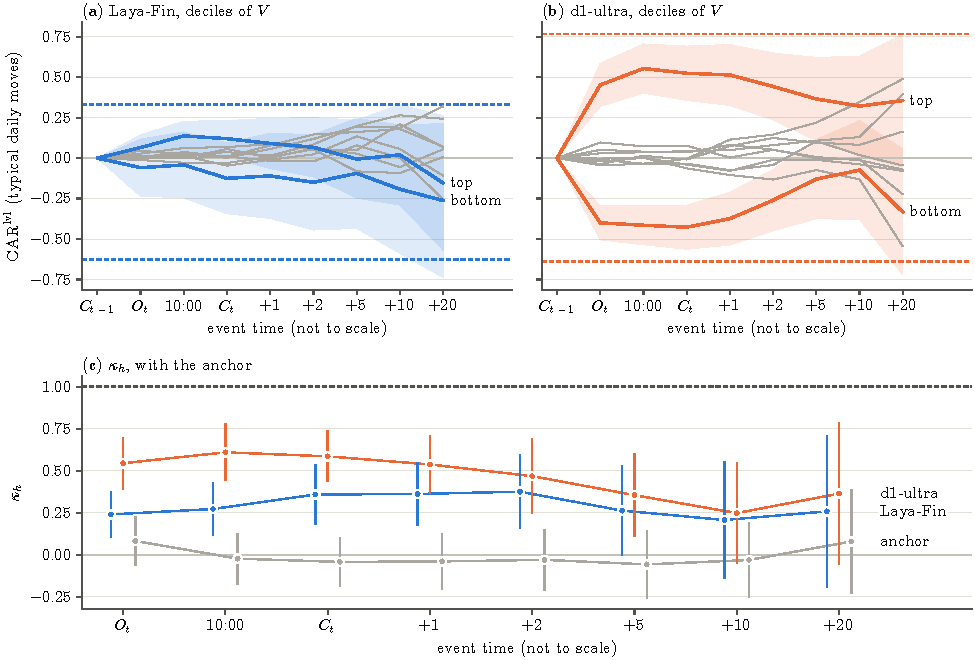
\includegraphics{figA7_convergence_detail.pdf}
\caption{\textbf{Convergence in detail, every decile and the anchor.} (a, b) $\mathrm{CAR}^{\mathrm{lvl}}$ of every decile of $V$ for Laya-Fin and d1-ultra (gray: deciles 2 to 9; the extreme deciles with SE bands and their mean $V$ dashed), on one scale. Laya-Fin's deciles are ordered like d1-ultra's but smaller and noisier: its top decile (mean $V$ 0.33) stands at +0.12 at the close. (c) The ladder $\kappa_h$ with the anchor, whose readings are uninformative (near-constant outputs): its $\kappa_h$ is about zero throughout ($-$0.04 at the close). Event time is not to scale; d1-ultra is model-specific (\S{}1.3).}\label{fig:figA7_convergence_detail}
\end{figure}

\clearpage

\begin{figure}[htbp]
\centering
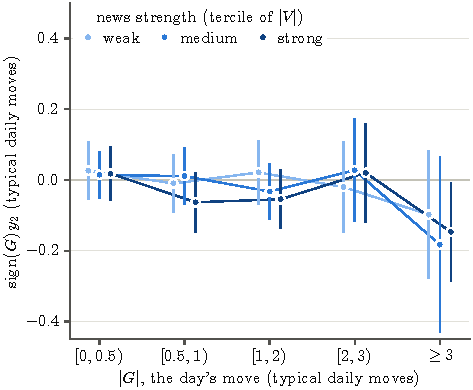
\includegraphics{figA8_drift_laya_fin.pdf}
\caption{\textbf{Laya-Fin's drift after the close by the size of the move.} Figure 4 (b) for Laya-Fin: $\mathrm{sign}(G)\,y_2$ by bin of $|G|$, one line per tercile of news strength $|V|$, with 95\% intervals. Moves with $|G| \geq 3$ reverse slightly in every tercile (strong $-$0.15, medium $-$0.18, weak $-$0.10); smaller moves do not drift.}\label{fig:figA8_drift_laya_fin}
\end{figure}

\clearpage

\begin{figure}[htbp]
\centering
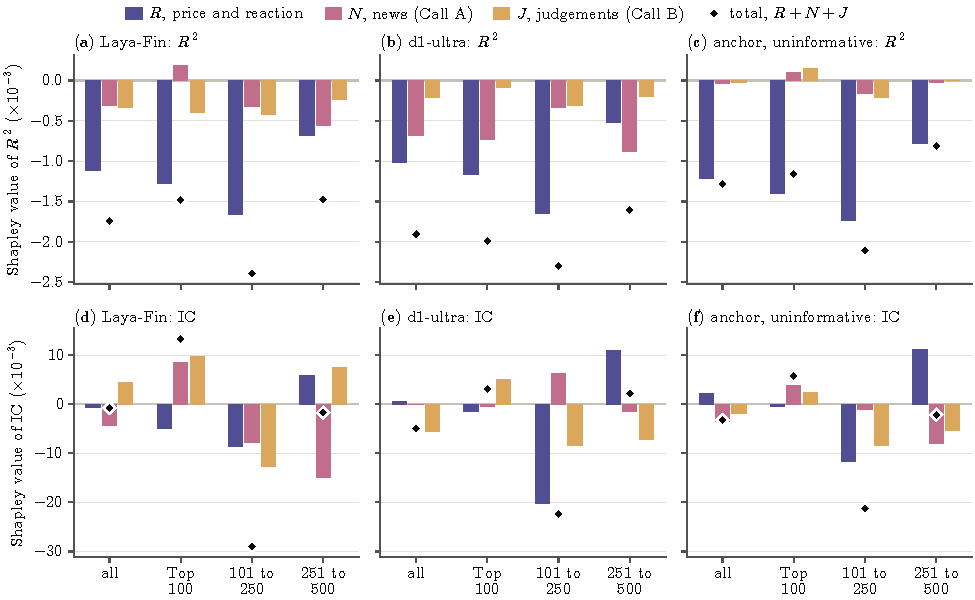
\includegraphics{figA9_shapley.pdf}
\caption{\textbf{The value of information at the close is about zero for every feature group.} Exact Shapley values of the test-period out-of-sample $R^2$ (a to c) and mean daily IC (d to f) of $y_2$ at D2 over the feature groups $R$ (price and reaction), $N$ (news, Call A) and $J$ (judgements, Call B), for all member-days and by size tier, with the full model's total $R + N + J$ (diamond), from the H3 ridge fits (\S{}11.5); values in units of $10^{-3}$, and each row on one scale. One column per instrument: Laya-Fin, d1-ultra (model-specific) and the anchor (uninformative, near-constant outputs). Every $R^2$ total is negative, in every tier; for all member-days it is $-$0.0017 for Laya-Fin, $-$0.0019 for d1-ultra and $-$0.0013 for the anchor, so the Shapley shares are shares of nothing and are not drawn. The IC totals are small and of both signs, from $-$0.029 (Laya-Fin, 101 to 250) to 0.013 (Laya-Fin, Top-100). H3 is not supported for Laya-Fin (Holm p 0.269).}\label{fig:figA9_shapley}
\end{figure}

\clearpage

\begin{figure}[htbp]
\centering
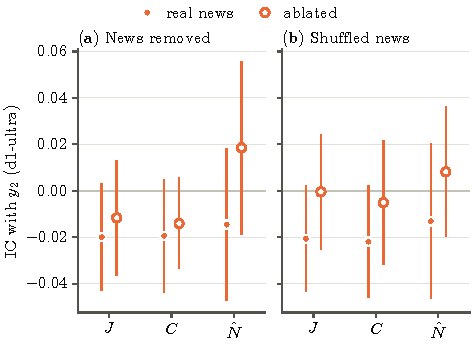
\includegraphics{figA10_ablations.pdf}
\caption{\textbf{Call B's judgments carry no information about the drift, with or without the news.} Call B ablations for d1-ultra (S8, on the same test events): the IC of $J$, $C$ and $\hat N$ with $y_2$, real news (filled) against (a) the news removed and (b) shuffled news (hollow), with 95\% intervals ($\pm$1.96 Newey--West SE). $J$'s IC is $-$0.02 with the news and $-$0.01 without it, and $-$0.02 against $-$0.00 with shuffled news. d1-ultra is model-specific (\S{}1.3).}\label{fig:figA10_ablations}
\end{figure}

\clearpage

% t2_h2_over_under (NA-14, from artifacts/NA-12/tables/t2_h2_over_under.csv)
\begin{table*}[tbp]
\centering\small
\caption{Over/under regression y = a + b$\cdot$\^{N} + c$\cdot$G + day $\times$ tier FE by decision point and within $|$G$|$ bins}\label{tab:t2_h2_over_under}
\begin{adjustbox}{max width=\textwidth}
\begin{tabular}{lllrrrrrrrrrrrrrrrrrrrl}
\toprule
model & variant & available & b & b SE & b t & b p & b SE DK & b p DK & c & c SE & c t & c p & c SE DK & c p DK & p & p DK & nobs & n sessions & n firms & df t & R\textsuperscript{2} within & reason \\
\midrule
Laya-Fin & D2 & yes & $-0.044$ & $0.149$ & $-0.295$ & $0.616$ & $0.150$ & $0.615$ & $-0.015$ & $0.012$ & $-1.235$ & $0.110$ & $0.012$ & $0.117$ & $0.616$ & $0.615$ & $17{,}188$ & $135$ & $500$ & $134$ & $2.90\times 10^{-4}$ & --- \\
Laya-Fin & D1 & yes & $0.229$ & $0.148$ & $1.550$ & $0.062$ & $0.183$ & $0.105$ & $0.013$ & $0.012$ & $1.088$ & $0.861$ & $0.014$ & $0.824$ & $0.861$ & $0.824$ & $13{,}203$ & $138$ & $496$ & $137$ & $7.10\times 10^{-4}$ & --- \\
Laya-Fin & D0 & yes & $0.278$ & $0.212$ & $1.311$ & $0.096$ & $0.237$ & $0.121$ & --- & --- & --- & --- & --- & --- & $0.096$ & $0.121$ & $13{,}439$ & $138$ & $500$ & $137$ & $4.02\times 10^{-4}$ & --- \\
Laya-Fin & D2, $|$G$|$ in [0, 1) & yes & $-0.187$ & $0.242$ & $-0.773$ & $0.779$ & $0.266$ & $0.758$ & $-0.016$ & $0.037$ & $-0.419$ & $0.338$ & $0.036$ & $0.330$ & $0.779$ & $0.758$ & $9{,}795$ & $135$ & $500$ & $134$ & $1.36\times 10^{-4}$ & --- \\
Laya-Fin & D2, $|$G$|$ in [1, 2) & yes & $-0.172$ & $0.273$ & $-0.629$ & $0.735$ & $0.272$ & $0.736$ & $-0.025$ & $0.026$ & $-0.956$ & $0.171$ & $0.027$ & $0.179$ & $0.735$ & $0.736$ & $4{,}647$ & $135$ & $496$ & $134$ & $5.75\times 10^{-4}$ & --- \\
Laya-Fin & D2, $|$G$|$ in [2, inf) & yes & $0.092$ & $0.254$ & $0.364$ & $0.358$ & $0.191$ & $0.315$ & $-0.013$ & $0.012$ & $-1.092$ & $0.138$ & $0.013$ & $0.157$ & $0.358$ & $0.315$ & $2{,}746$ & $135$ & $486$ & $134$ & $0.001$ & --- \\
anchor (uninformative) & D2 & yes & $0.748$ & $1.377$ & $0.543$ & $0.294$ & $1.827$ & $0.341$ & $-0.015$ & $0.012$ & $-1.228$ & $0.111$ & $0.013$ & $0.121$ & $0.294$ & $0.341$ & $17{,}188$ & $135$ & $500$ & $134$ & $2.94\times 10^{-4}$ & --- \\
anchor (uninformative) & D1 & yes & $1.964$ & $2.482$ & $0.791$ & $0.215$ & $3.175$ & $0.269$ & $0.014$ & $0.012$ & $1.152$ & $0.874$ & $0.014$ & $0.838$ & $0.874$ & $0.838$ & $13{,}203$ & $138$ & $496$ & $137$ & $5.42\times 10^{-4}$ & --- \\
anchor (uninformative) & D0 & yes & $-4.510$ & $3.236$ & $-1.394$ & $0.917$ & $3.541$ & $0.898$ & --- & --- & --- & --- & --- & --- & $0.917$ & $0.898$ & $13{,}439$ & $138$ & $500$ & $137$ & $6.68\times 10^{-4}$ & --- \\
anchor (uninformative) & D2, $|$G$|$ in [0, 1) & yes & $-0.086$ & $3.523$ & $-0.025$ & $0.510$ & $2.601$ & $0.513$ & $-0.016$ & $0.037$ & $-0.439$ & $0.331$ & $0.036$ & $0.323$ & $0.510$ & $0.513$ & $9{,}795$ & $135$ & $500$ & $134$ & $3.05\times 10^{-5}$ & --- \\
anchor (uninformative) & D2, $|$G$|$ in [1, 2) & yes & $1.336$ & $3.596$ & $0.372$ & $0.355$ & $4.047$ & $0.371$ & $-0.026$ & $0.026$ & $-0.972$ & $0.167$ & $0.027$ & $0.174$ & $0.355$ & $0.371$ & $4{,}647$ & $135$ & $496$ & $134$ & $4.95\times 10^{-4}$ & --- \\
anchor (uninformative) & D2, $|$G$|$ in [2, inf) & yes & $0.273$ & $2.604$ & $0.105$ & $0.458$ & $2.445$ & $0.456$ & $-0.013$ & $0.012$ & $-1.039$ & $0.150$ & $0.013$ & $0.168$ & $0.458$ & $0.456$ & $2{,}746$ & $135$ & $486$ & $134$ & $9.95\times 10^{-4}$ & --- \\
Laya zero-shot & D2 & no & --- & --- & --- & --- & --- & --- & --- & --- & --- & --- & --- & --- & --- & --- & --- & --- & --- & --- & --- & no Call A W2 reading \\
Laya zero-shot & D1 & yes & $-6.53\times 10^{-4}$ & $0.063$ & $-0.010$ & $0.504$ & $0.068$ & $0.504$ & $0.014$ & $0.012$ & $1.134$ & $0.871$ & $0.014$ & $0.833$ & $0.871$ & $0.833$ & $13{,}203$ & $138$ & $496$ & $137$ & $4.02\times 10^{-4}$ & --- \\
Laya zero-shot & D0 & yes & $-0.021$ & $0.069$ & $-0.305$ & $0.619$ & $0.077$ & $0.608$ & --- & --- & --- & --- & --- & --- & $0.619$ & $0.608$ & $13{,}439$ & $138$ & $500$ & $137$ & $1.26\times 10^{-5}$ & --- \\
d1-ultra & D2 & yes & $-0.076$ & $0.031$ & $-2.409$ & $0.991$ & $0.034$ & $0.985$ & $-0.011$ & $0.012$ & $-0.954$ & $0.171$ & $0.012$ & $0.175$ & $0.991$ & $0.985$ & $17{,}188$ & $135$ & $500$ & $134$ & $0.001$ & --- \\
d1-ultra & D1 & yes & $-0.018$ & $0.032$ & $-0.558$ & $0.711$ & $0.032$ & $0.707$ & $0.015$ & $0.012$ & $1.201$ & $0.884$ & $0.014$ & $0.853$ & $0.884$ & $0.853$ & $13{,}203$ & $138$ & $496$ & $137$ & $4.54\times 10^{-4}$ & --- \\
d1-ultra & D0 & yes & $0.022$ & $0.037$ & $0.595$ & $0.277$ & $0.037$ & $0.280$ & --- & --- & --- & --- & --- & --- & $0.277$ & $0.280$ & $13{,}439$ & $138$ & $500$ & $137$ & $7.08\times 10^{-5}$ & --- \\
d1-ultra & D2, $|$G$|$ in [0, 1) & yes & $-0.067$ & $0.043$ & $-1.556$ & $0.939$ & $0.053$ & $0.898$ & $-0.015$ & $0.037$ & $-0.391$ & $0.348$ & $0.035$ & $0.340$ & $0.939$ & $0.898$ & $9{,}795$ & $135$ & $500$ & $134$ & $5.54\times 10^{-4}$ & --- \\
d1-ultra & D2, $|$G$|$ in [1, 2) & yes & $-0.086$ & $0.053$ & $-1.626$ & $0.947$ & $0.045$ & $0.972$ & $-0.023$ & $0.026$ & $-0.883$ & $0.189$ & $0.027$ & $0.196$ & $0.947$ & $0.972$ & $4{,}647$ & $135$ & $496$ & $134$ & $0.001$ & --- \\
d1-ultra & D2, $|$G$|$ in [2, inf) & yes & $-0.080$ & $0.056$ & $-1.416$ & $0.920$ & $0.049$ & $0.948$ & $-0.009$ & $0.013$ & $-0.719$ & $0.237$ & $0.013$ & $0.249$ & $0.920$ & $0.948$ & $2{,}746$ & $135$ & $486$ & $134$ & $0.002$ & --- \\
span-02\textsuperscript{\ddag} & D2 & no & --- & --- & --- & --- & --- & --- & --- & --- & --- & --- & --- & --- & --- & --- & --- & --- & --- & --- & --- & no Call A W2 reading \\
span-02\textsuperscript{\ddag} & D1 & yes & $-0.010$ & $0.023$ & $-0.431$ & $0.666$ & $0.024$ & $0.660$ & $0.014$ & $0.012$ & $1.188$ & $0.882$ & $0.014$ & $0.850$ & $0.882$ & $0.850$ & $13{,}203$ & $138$ & $496$ & $137$ & $4.39\times 10^{-4}$ & --- \\
span-02\textsuperscript{\ddag} & D0 & yes & $0.013$ & $0.023$ & $0.578$ & $0.282$ & $0.024$ & $0.293$ & --- & --- & --- & --- & --- & --- & $0.282$ & $0.293$ & $13{,}439$ & $138$ & $500$ & $137$ & $5.88\times 10^{-5}$ & --- \\
drex-v2.0 & D2 & no & --- & --- & --- & --- & --- & --- & --- & --- & --- & --- & --- & --- & --- & --- & --- & --- & --- & --- & --- & no Call A W2 reading \\
drex-v2.0 & D1 & yes & $-0.032$ & $0.026$ & $-1.227$ & $0.889$ & $0.029$ & $0.859$ & $0.015$ & $0.012$ & $1.231$ & $0.890$ & $0.014$ & $0.857$ & $0.890$ & $0.859$ & $13{,}203$ & $138$ & $496$ & $137$ & $6.00\times 10^{-4}$ & --- \\
drex-v2.0 & D0 & yes & $0.011$ & $0.030$ & $0.370$ & $0.356$ & $0.030$ & $0.354$ & --- & --- & --- & --- & --- & --- & $0.356$ & $0.354$ & $13{,}439$ & $138$ & $500$ & $137$ & $2.14\times 10^{-5}$ & --- \\
\bottomrule
\end{tabular}
\end{adjustbox}
\par\smallskip{\footnotesize\raggedright Two-way clustered (session, firm) SEs; Driscoll--Kraay (5 lags) SEs and p in the \_dk columns. D2: y2, G = z\_cc,t, \^{N} from Call A on W2; D1: y1, G at 10:00, \^{N}\_W0; D0: y0 = z\_id, no G. The anchor's readings are uninformative (near-constant outputs: NA-11 REPORT \S{}7.1 item 4); its rows are reported, not read as nulls. \textsuperscript{\ddag} span-02: the S5 canary fired a STOP after the freeze; the operator chose to proceed (PREREG \S{}15, the post-freeze NA-11 S5 row).\par}
\end{table*}


\clearpage

% t4_secondary (NA-14, from artifacts/NA-12/tables/t4_secondary.csv)
\begin{table*}[tbp]
\centering\small
\caption{Secondary hypotheses (BH, q = 0.10, within each instrument; pooled sensitivity family)}\label{tab:t4_secondary}
\begin{adjustbox}{max width=\textwidth}
\begin{tabular}{lllrrlrr>{\raggedright\arraybackslash}p{12em}rrrr}
\toprule
model & test & available & estimate & p & in family & q & q pooled & reason & CI low & CI high & SE & nobs \\
\midrule
Laya-Fin & H5 & yes & $0.002$ & $0.010$ & yes & $0.058$ & $0.078$ & --- & --- & --- & --- & --- \\
Laya-Fin & H6 & no & --- & --- & --- & --- & --- & no tone or materiality (Q3--Q4) & --- & --- & --- & --- \\
Laya-Fin & H7 & yes & $0.015$ & $0.097$ & yes & $0.238$ & $0.317$ & --- & $-0.007$ & $0.036$ & --- & --- \\
Laya-Fin & H2C\_kappa\_hstar & yes & $0.259$ & $0.131$ & yes & $0.238$ & $0.317$ & --- & --- & --- & $0.230$ & $11{,}201$ \\
Laya-Fin & H2C\_kappa\_increase & yes & $0.018$ & $0.467$ & yes & $0.561$ & $0.748$ & --- & $-0.361$ & $0.490$ & --- & --- \\
Laya-Fin & H2C\_lambda\_t5 & yes & $0.026$ & $0.159$ & yes & $0.238$ & $0.317$ & --- & --- & --- & $0.026$ & $17{,}188$ \\
Laya-Fin & H2C\_tracking\_naive & yes & $1.001$ & $0.867$ & yes & $0.867$ & $0.946$ & --- & $0.999$ & $1.002$ & --- & --- \\
Laya-Fin & A3.4 & no & --- & --- & --- & --- & --- & no explanation answer X (Q16) & --- & --- & --- & --- \\
anchor (uninformative) & H5 & yes & $3.29\times 10^{-4}$ & $0.072$ & yes & $0.358$ & --- & --- & --- & --- & --- & --- \\
anchor (uninformative) & H6 & no & --- & --- & --- & --- & --- & no tone or materiality (Q3--Q4) & --- & --- & --- & --- \\
anchor (uninformative) & H7 & yes & $0.002$ & $0.442$ & no & --- & --- & --- & $-0.029$ & $0.036$ & --- & --- \\
anchor (uninformative) & H2C\_kappa\_hstar & yes & $0.080$ & $0.307$ & yes & $0.511$ & --- & --- & --- & --- & $0.157$ & $11{,}201$ \\
anchor (uninformative) & H2C\_kappa\_increase & yes & $-0.003$ & $0.514$ & yes & $0.643$ & --- & --- & $-0.267$ & $0.422$ & --- & --- \\
anchor (uninformative) & H2C\_lambda\_t5 & yes & $0.027$ & $0.156$ & yes & $0.390$ & --- & --- & --- & --- & $0.027$ & $17{,}188$ \\
anchor (uninformative) & H2C\_tracking\_naive & yes & $1.002$ & $0.992$ & yes & $0.992$ & --- & --- & $1.000$ & $1.004$ & --- & --- \\
anchor (uninformative) & A3.4 & no & --- & --- & --- & --- & --- & no explanation answer X (Q16) & --- & --- & --- & --- \\
d1-ultra & H5 & yes & $0.008$ & $<0.001$ & yes & $<0.001$ & --- & --- & --- & --- & --- & --- \\
d1-ultra & H6 & yes & $0.010$ & $0.705$ & yes & $0.946$ & $0.940$ & --- & --- & --- & $0.019$ & $17{,}188$ \\
d1-ultra & H7 & no & --- & --- & --- & --- & --- & H7 compares a trained model with Laya zero-shot & --- & --- & --- & --- \\
d1-ultra & H2C\_kappa\_hstar & yes & $0.365$ & $0.046$ & yes & $0.163$ & --- & --- & --- & --- & $0.215$ & $11{,}201$ \\
d1-ultra & H2C\_kappa\_increase & yes & $-0.181$ & $0.834$ & yes & $0.946$ & --- & --- & $-0.534$ & $0.216$ & --- & --- \\
d1-ultra & H2C\_lambda\_t5 & yes & $0.022$ & $0.206$ & yes & $0.480$ & --- & --- & --- & --- & $0.026$ & $17{,}188$ \\
d1-ultra & H2C\_tracking\_naive & yes & $1.000$ & $0.781$ & yes & $0.946$ & --- & --- & $0.999$ & $1.002$ & --- & --- \\
d1-ultra & A3.4 & yes & $-0.062$ & $0.946$ & yes & $0.946$ & $0.946$ & --- & --- & --- & $0.038$ & $17{,}188$ \\
\bottomrule
\end{tabular}
\end{adjustbox}
\par\smallskip{\footnotesize\raggedright H6 and A3.4 need tone and the explanation answer (Q16), which the trained models do not give. The pooled family adds d1-ultra's H6 and A3.4 to Laya-Fin's six (PREREG \S{}15 NA-12 row). The anchor's readings are uninformative (near-constant outputs: NA-11 REPORT \S{}7.1 item 4); its rows are reported, not read as nulls.\par}
\end{table*}


\clearpage

% t5_heterogeneity (NA-14, from artifacts/NA-12/tables/t5_heterogeneity.csv)
\begin{table*}[tbp]
\centering\small
\caption{Heterogeneity cuts on H2 at D2: Wald test of \^{N}$\cdot$1[cut] and G$\cdot$1[cut], BH over each model's eight cuts}\label{tab:t5_heterogeneity}
\begin{adjustbox}{max width=\textwidth}
\begin{tabular}{llrrrrrrrrrrrrrrrrrrrrrrrr}
\toprule
model & cut & n in & n out & wald f & wald q & p & b diff & b diff SE & b diff t & b diff SE DK & b diff p two & c diff & c diff SE & c diff t & c diff SE DK & c diff p two & b in & b in SE & c in & c in SE & b out & b out SE & c out & c out SE & q \\
\midrule
Laya-Fin & tier\_top100 & $4{,}516$ & $12{,}672$ & $1.832$ & $2$ & $0.164$ & $0.490$ & $0.281$ & $1.741$ & $0.272$ & $0.084$ & $-0.025$ & $0.021$ & $-1.196$ & $0.030$ & $0.234$ & $0.341$ & $0.270$ & $-0.034$ & $0.020$ & $-0.149$ & $0.162$ & $-0.009$ & $0.013$ & $0.741$ \\
Laya-Fin & tier\_mid & $5{,}121$ & $12{,}067$ & $0.102$ & $2$ & $0.904$ & $-0.008$ & $0.258$ & $-0.031$ & $0.265$ & $0.976$ & $-0.007$ & $0.016$ & $-0.441$ & $0.014$ & $0.660$ & $-0.049$ & $0.246$ & $-0.020$ & $0.016$ & $-0.042$ & $0.161$ & $-0.013$ & $0.013$ & $0.904$ \\
Laya-Fin & tier\_rest & $7{,}551$ & $9{,}637$ & $1.708$ & $2$ & $0.185$ & $-0.326$ & $0.253$ & $-1.285$ & $0.283$ & $0.201$ & $0.023$ & $0.016$ & $1.473$ & $0.019$ & $0.143$ & $-0.217$ & $0.189$ & $-0.003$ & $0.015$ & $0.108$ & $0.201$ & $-0.026$ & $0.014$ & $0.741$ \\
Laya-Fin & quantified & $15{,}030$ & $2{,}158$ & $0.656$ & $2$ & $0.521$ & $0.470$ & $0.609$ & $0.773$ & $0.582$ & $0.441$ & $0.022$ & $0.026$ & $0.832$ & $0.023$ & $0.407$ & $-0.015$ & $0.154$ & $-0.013$ & $0.013$ & $-0.156$ & $0.613$ & $-0.037$ & $0.030$ & $0.833$ \\
Laya-Fin & small\_move & $9{,}795$ & $7{,}393$ & $0.286$ & $2$ & $0.751$ & $-0.193$ & $0.255$ & $-0.756$ & $0.239$ & $0.451$ & $0.005$ & $0.035$ & $0.154$ & $0.035$ & $0.878$ & $-0.187$ & $0.242$ & $-0.016$ & $0.037$ & $0.048$ & $0.180$ & $-0.016$ & $0.012$ & $0.859$ \\
Laya-Fin & press\_wire & $9{,}655$ & $7{,}533$ & $0.745$ & $2$ & $0.477$ & $-0.058$ & $0.330$ & $-0.176$ & $0.304$ & $0.860$ & $-0.024$ & $0.020$ & $-1.166$ & $0.021$ & $0.246$ & $-0.062$ & $0.157$ & $-0.022$ & $0.012$ & $0.045$ & $0.306$ & $0.004$ & $0.022$ & $0.833$ \\
Laya-Fin & usual\_coverage\_low & $8{,}387$ & $8{,}769$ & $0.439$ & $2$ & $0.645$ & $0.040$ & $0.247$ & $0.162$ & $0.210$ & $0.872$ & $0.014$ & $0.016$ & $0.837$ & $0.013$ & $0.404$ & $-0.010$ & $0.196$ & $-0.011$ & $0.015$ & $-0.017$ & $0.204$ & $-0.022$ & $0.015$ & $0.859$ \\
Laya-Fin & busy\_day & $7{,}805$ & $9{,}351$ & $0.928$ & $2$ & $0.398$ & $-0.194$ & $0.263$ & $-0.736$ & $0.268$ & $0.463$ & $-0.019$ & $0.019$ & $-0.992$ & $0.019$ & $0.323$ & $-0.120$ & $0.179$ & $-0.026$ & $0.015$ & $0.105$ & $0.250$ & $-0.004$ & $0.017$ & $0.833$ \\
anchor (uninformative) & tier\_top100 & $4{,}516$ & $12{,}672$ & $2.178$ & $2$ & $0.117$ & $6.973$ & $4.120$ & $1.693$ & $3.356$ & $0.093$ & $-0.023$ & $0.020$ & $-1.129$ & $0.030$ & $0.261$ & $6.255$ & $3.068$ & $-0.033$ & $0.020$ & $-0.718$ & $1.843$ & $-0.010$ & $0.013$ & $0.469$ \\
anchor (uninformative) & tier\_mid & $5{,}121$ & $12{,}067$ & $0.523$ & $2$ & $0.594$ & $-2.559$ & $2.719$ & $-0.941$ & $2.803$ & $0.348$ & $-0.007$ & $0.016$ & $-0.467$ & $0.014$ & $0.641$ & $-1.045$ & $1.777$ & $-0.020$ & $0.016$ & $1.514$ & $1.904$ & $-0.013$ & $0.013$ & $0.679$ \\
anchor (uninformative) & tier\_rest & $7{,}551$ & $9{,}637$ & $1.175$ & $2$ & $0.312$ & $-2.500$ & $3.035$ & $-0.824$ & $2.754$ & $0.412$ & $0.021$ & $0.015$ & $1.399$ & $0.019$ & $0.164$ & $-0.590$ & $2.656$ & $-0.004$ & $0.015$ & $1.910$ & $1.278$ & $-0.025$ & $0.014$ & $0.679$ \\
anchor (uninformative) & quantified & $15{,}030$ & $2{,}158$ & $2.838$ & $2$ & $0.062$ & $7.109$ & $3.308$ & $2.149$ & $3.171$ & $0.033$ & $0.024$ & $0.026$ & $0.901$ & $0.023$ & $0.369$ & $1.112$ & $1.346$ & $-0.013$ & $0.013$ & $-7.930$ & $11.920$ & $-0.036$ & $0.031$ & $0.469$ \\
anchor (uninformative) & small\_move & $9{,}795$ & $7{,}393$ & $0.008$ & $2$ & $0.992$ & $0.018$ & $2.650$ & $0.007$ & $2.630$ & $0.995$ & $0.004$ & $0.035$ & $0.128$ & $0.035$ & $0.898$ & $-0.086$ & $3.523$ & $-0.016$ & $0.037$ & $0.819$ & $2.229$ & $-0.016$ & $0.012$ & $0.992$ \\
anchor (uninformative) & press\_wire & $9{,}655$ & $7{,}533$ & $0.788$ & $2$ & $0.457$ & $-1.650$ & $3.084$ & $-0.535$ & $2.590$ & $0.594$ & $-0.024$ & $0.020$ & $-1.175$ & $0.021$ & $0.242$ & $0.251$ & $1.575$ & $-0.022$ & $0.012$ & $5.365$ & $7.674$ & $0.003$ & $0.022$ & $0.679$ \\
anchor (uninformative) & usual\_coverage\_low & $8{,}387$ & $8{,}769$ & $0.745$ & $2$ & $0.477$ & $2.272$ & $2.652$ & $0.856$ & $2.588$ & $0.393$ & $0.014$ & $0.016$ & $0.874$ & $0.013$ & $0.384$ & $-0.684$ & $2.080$ & $-0.011$ & $0.015$ & $2.390$ & $2.242$ & $-0.022$ & $0.015$ & $0.679$ \\
anchor (uninformative) & busy\_day & $7{,}805$ & $9{,}351$ & $0.580$ & $2$ & $0.561$ & $1.140$ & $2.570$ & $0.444$ & $2.519$ & $0.658$ & $-0.020$ & $0.019$ & $-1.031$ & $0.019$ & $0.305$ & $0.726$ & $1.717$ & $-0.026$ & $0.015$ & $3.294$ & $2.958$ & $-0.003$ & $0.017$ & $0.679$ \\
d1-ultra & tier\_top100 & $4{,}516$ & $12{,}672$ & $1.096$ & $2$ & $0.337$ & $0.059$ & $0.060$ & $0.987$ & $0.060$ & $0.326$ & $-0.024$ & $0.020$ & $-1.187$ & $0.030$ & $0.237$ & $-0.030$ & $0.052$ & $-0.030$ & $0.020$ & $-0.089$ & $0.036$ & $-0.006$ & $0.013$ & $0.719$ \\
d1-ultra & tier\_mid & $5{,}121$ & $12{,}067$ & $0.878$ & $2$ & $0.418$ & $0.063$ & $0.055$ & $1.150$ & $0.044$ & $0.252$ & $-0.010$ & $0.016$ & $-0.661$ & $0.014$ & $0.510$ & $-0.031$ & $0.050$ & $-0.019$ & $0.016$ & $-0.094$ & $0.035$ & $-0.008$ & $0.013$ & $0.719$ \\
d1-ultra & tier\_rest & $7{,}551$ & $9{,}637$ & $3.362$ & $2$ & $0.038$ & $-0.095$ & $0.050$ & $-1.895$ & $0.037$ & $0.060$ & $0.026$ & $0.015$ & $1.691$ & $0.019$ & $0.093$ & $-0.126$ & $0.043$ & $0.002$ & $0.015$ & $-0.031$ & $0.037$ & $-0.024$ & $0.014$ & $0.301$ \\
d1-ultra & quantified & $15{,}030$ & $2{,}158$ & $0.529$ & $2$ & $0.591$ & $0.014$ & $0.062$ & $0.225$ & $0.056$ & $0.822$ & $0.023$ & $0.027$ & $0.868$ & $0.023$ & $0.387$ & $-0.084$ & $0.033$ & $-0.009$ & $0.012$ & $-6.28\times 10^{-4}$ & $0.079$ & $-0.038$ & $0.031$ & $0.719$ \\
d1-ultra & small\_move & $9{,}795$ & $7{,}393$ & $0.155$ & $2$ & $0.857$ & $0.023$ & $0.044$ & $0.534$ & $0.040$ & $0.594$ & $0.002$ & $0.035$ & $0.070$ & $0.035$ & $0.945$ & $-0.067$ & $0.043$ & $-0.015$ & $0.037$ & $-0.084$ & $0.039$ & $-0.012$ & $0.012$ & $0.857$ \\
d1-ultra & press\_wire & $9{,}655$ & $7{,}533$ & $0.667$ & $2$ & $0.515$ & $-0.021$ & $0.049$ & $-0.420$ & $0.054$ & $0.675$ & $-0.022$ & $0.020$ & $-1.136$ & $0.020$ & $0.258$ & $-0.076$ & $0.034$ & $-0.018$ & $0.012$ & $-0.049$ & $0.049$ & $0.006$ & $0.021$ & $0.719$ \\
d1-ultra & usual\_coverage\_low & $8{,}387$ & $8{,}769$ & $2.523$ & $2$ & $0.084$ & $0.096$ & $0.046$ & $2.076$ & $0.035$ & $0.040$ & $0.010$ & $0.016$ & $0.602$ & $0.013$ & $0.548$ & $-0.037$ & $0.042$ & $-0.009$ & $0.014$ & $-0.117$ & $0.041$ & $-0.017$ & $0.015$ & $0.336$ \\
d1-ultra & busy\_day & $7{,}805$ & $9{,}351$ & $0.466$ & $2$ & $0.629$ & $0.002$ & $0.043$ & $0.056$ & $0.052$ & $0.955$ & $-0.019$ & $0.019$ & $-0.965$ & $0.019$ & $0.336$ & $-0.079$ & $0.037$ & $-0.022$ & $0.015$ & $-0.066$ & $0.041$ & $-0.001$ & $0.017$ & $0.719$ \\
\bottomrule
\end{tabular}
\end{adjustbox}
\par\smallskip{\footnotesize\raggedright Laya-Fin's eight cuts are the family; the anchor's and d1-ultra's are reported. The anchor's readings are uninformative (near-constant outputs: NA-11 REPORT \S{}7.1 item 4); its rows are reported, not read as nulls.\par}
\end{table*}


\clearpage

% t6_convergence_ladder (NA-14, from artifacts/NA-12/tables/t6_convergence_ladder.csv)
\begin{landscape}
{\scriptsize\setlength{\tabcolsep}{3pt}
\begin{longtable}{llllrrrrrrrrrr}
\caption{A1 convergence ladder: $\kappa$\_h of CAR\textasciicircum{}lvl\_h on V (D0 events, day $\times$ tier FE) and the shares $\kappa$\_h / $\kappa$\_h*}\label{tab:t6_convergence_ladder}\\
\toprule
model & variant & rung & available & kappa & kappa SE & kappa t & kappa p & kappa SE DK & kappa p DK & share of h star & nobs & CI low & CI high \\
\midrule
\endfirsthead
\toprule
model & variant & rung & available & kappa & kappa SE & kappa t & kappa p & kappa SE DK & kappa p DK & share of h star & nobs & CI low & CI high \\
\midrule
\endhead
\bottomrule
\endfoot
Laya-Fin & ladder & O\_t & yes & $0.241$ & $0.070$ & $3.446$ & $<0.001$ & $0.069$ & $<0.001$ & $0.929$ & $13{,}439$ & --- & --- \\
Laya-Fin & ladder & 10:00 & yes & $0.273$ & $0.080$ & $3.404$ & $<0.001$ & $0.081$ & $<0.001$ & $1.055$ & $13{,}287$ & --- & --- \\
Laya-Fin & ladder & C\_t & yes & $0.359$ & $0.090$ & $3.973$ & $<0.001$ & $0.108$ & $<0.001$ & $1.387$ & $13{,}748$ & --- & --- \\
Laya-Fin & ladder & C\_t+1 & yes & $0.362$ & $0.097$ & $3.755$ & $<0.001$ & $0.100$ & $<0.001$ & $1.400$ & $13{,}615$ & --- & --- \\
Laya-Fin & ladder & C\_t+2 & yes & $0.376$ & $0.112$ & $3.358$ & $<0.001$ & $0.111$ & $<0.001$ & $1.453$ & $13{,}439$ & --- & --- \\
Laya-Fin & ladder & C\_t+5 & yes & $0.263$ & $0.137$ & $1.915$ & $0.029$ & $0.134$ & $0.026$ & $1.017$ & $12{,}850$ & --- & --- \\
Laya-Fin & ladder & C\_t+10 & yes & $0.208$ & $0.177$ & $1.175$ & $0.121$ & $0.179$ & $0.124$ & $0.803$ & $11{,}993$ & --- & --- \\
Laya-Fin & ladder & C\_t+20 & yes & $0.259$ & $0.230$ & $1.126$ & $0.131$ & $0.234$ & $0.136$ & $1.000$ & $11{,}201$ & --- & --- \\
Laya-Fin & ladder & O\_t $\to$ C\_t+20 & yes & $0.018$ & --- & --- & $0.467$ & --- & --- & --- & --- & $-0.361$ & $0.490$ \\
Laya-Fin & ladder\_clean & O\_t & yes & $0.241$ & $0.070$ & $3.446$ & $<0.001$ & $0.069$ & $<0.001$ & $-0.337$ & $13{,}439$ & --- & --- \\
Laya-Fin & ladder\_clean & 10:00 & yes & $0.273$ & $0.080$ & $3.404$ & $<0.001$ & $0.081$ & $<0.001$ & $-0.382$ & $13{,}287$ & --- & --- \\
Laya-Fin & ladder\_clean & C\_t & yes & $0.359$ & $0.090$ & $3.973$ & $<0.001$ & $0.108$ & $<0.001$ & $-0.502$ & $13{,}748$ & --- & --- \\
Laya-Fin & ladder\_clean & C\_t+1 & yes & $0.325$ & $0.166$ & $1.956$ & $0.026$ & $0.162$ & $0.024$ & $-0.455$ & $7{,}705$ & --- & --- \\
Laya-Fin & ladder\_clean & C\_t+2 & yes & $0.538$ & $0.279$ & $1.926$ & $0.028$ & $0.289$ & $0.033$ & $-0.752$ & $5{,}130$ & --- & --- \\
Laya-Fin & ladder\_clean & C\_t+5 & yes & $0.114$ & $0.346$ & $0.330$ & $0.371$ & $0.382$ & $0.383$ & $-0.160$ & $2{,}091$ & --- & --- \\
Laya-Fin & ladder\_clean & C\_t+10 & yes & $0.338$ & $1.005$ & $0.336$ & $0.369$ & $0.924$ & $0.358$ & $-0.473$ & $853$ & --- & --- \\
Laya-Fin & ladder\_clean & C\_t+20 & yes & $-0.715$ & $4.653$ & $-0.154$ & $0.561$ & $5.147$ & $0.555$ & $1.000$ & $205$ & --- & --- \\
Laya-Fin & ladder\_clean & O\_t $\to$ C\_t+20 & yes & $-0.955$ & --- & --- & $0.550$ & --- & --- & --- & --- & $-15.232$ & $3.291$ \\
Laya-Fin & ladder\_h10 & O\_t & yes & $0.241$ & $0.070$ & $3.446$ & $<0.001$ & $0.069$ & $<0.001$ & $1.158$ & $13{,}439$ & --- & --- \\
Laya-Fin & ladder\_h10 & 10:00 & yes & $0.273$ & $0.080$ & $3.404$ & $<0.001$ & $0.081$ & $<0.001$ & $1.314$ & $13{,}287$ & --- & --- \\
Laya-Fin & ladder\_h10 & C\_t & yes & $0.359$ & $0.090$ & $3.973$ & $<0.001$ & $0.108$ & $<0.001$ & $1.728$ & $13{,}748$ & --- & --- \\
Laya-Fin & ladder\_h10 & C\_t+1 & yes & $0.362$ & $0.097$ & $3.755$ & $<0.001$ & $0.100$ & $<0.001$ & $1.744$ & $13{,}615$ & --- & --- \\
Laya-Fin & ladder\_h10 & C\_t+2 & yes & $0.376$ & $0.112$ & $3.358$ & $<0.001$ & $0.111$ & $<0.001$ & $1.810$ & $13{,}439$ & --- & --- \\
Laya-Fin & ladder\_h10 & C\_t+5 & yes & $0.263$ & $0.137$ & $1.915$ & $0.029$ & $0.134$ & $0.026$ & $1.267$ & $12{,}850$ & --- & --- \\
Laya-Fin & ladder\_h10 & C\_t+10 & yes & $0.208$ & $0.177$ & $1.175$ & $0.121$ & $0.179$ & $0.124$ & $1.000$ & $11{,}993$ & --- & --- \\
Laya-Fin & ladder\_h10 & C\_t+20 & yes & $0.259$ & $0.230$ & $1.126$ & $0.131$ & $0.234$ & $0.136$ & $1.245$ & $11{,}201$ & --- & --- \\
Laya-Fin & ladder\_h10 & O\_t $\to$ C\_t+10 & yes & $-0.033$ & --- & --- & $0.581$ & --- & --- & --- & --- & $-0.408$ & $0.294$ \\
Laya-Fin & ladder\_plateau & plateau & yes & $0.273$ & $0.218$ & $1.253$ & $0.106$ & $0.223$ & $0.112$ & --- & $11{,}201$ & --- & --- \\
anchor (uninformative) & ladder & O\_t & yes & $0.083$ & $0.075$ & $1.101$ & $0.136$ & $0.080$ & $0.150$ & $1.039$ & $13{,}439$ & --- & --- \\
anchor (uninformative) & ladder & 10:00 & yes & $-0.022$ & $0.077$ & $-0.284$ & $0.612$ & $0.080$ & $0.608$ & $-0.276$ & $13{,}287$ & --- & --- \\
anchor (uninformative) & ladder & C\_t & yes & $-0.042$ & $0.074$ & $-0.560$ & $0.712$ & $0.080$ & $0.699$ & $-0.522$ & $13{,}748$ & --- & --- \\
anchor (uninformative) & ladder & C\_t+1 & yes & $-0.039$ & $0.086$ & $-0.449$ & $0.673$ & $0.088$ & $0.668$ & $-0.483$ & $13{,}615$ & --- & --- \\
anchor (uninformative) & ladder & C\_t+2 & yes & $-0.029$ & $0.092$ & $-0.320$ & $0.625$ & $0.084$ & $0.636$ & $-0.368$ & $13{,}439$ & --- & --- \\
anchor (uninformative) & ladder & C\_t+5 & yes & $-0.056$ & $0.103$ & $-0.546$ & $0.707$ & $0.108$ & $0.699$ & $-0.707$ & $12{,}850$ & --- & --- \\
anchor (uninformative) & ladder & C\_t+10 & yes & $-0.030$ & $0.114$ & $-0.264$ & $0.604$ & $0.116$ & $0.602$ & $-0.378$ & $11{,}993$ & --- & --- \\
anchor (uninformative) & ladder & C\_t+20 & yes & $0.080$ & $0.157$ & $0.507$ & $0.307$ & $0.193$ & $0.340$ & $1.000$ & $11{,}201$ & --- & --- \\
anchor (uninformative) & ladder & O\_t $\to$ C\_t+20 & yes & $-0.003$ & --- & --- & $0.514$ & --- & --- & --- & --- & $-0.267$ & $0.422$ \\
anchor (uninformative) & ladder\_clean & O\_t & yes & $0.083$ & $0.075$ & $1.101$ & $0.136$ & $0.080$ & $0.150$ & $0.012$ & $13{,}439$ & --- & --- \\
anchor (uninformative) & ladder\_clean & 10:00 & yes & $-0.022$ & $0.077$ & $-0.284$ & $0.612$ & $0.080$ & $0.608$ & $-0.003$ & $13{,}287$ & --- & --- \\
anchor (uninformative) & ladder\_clean & C\_t & yes & $-0.042$ & $0.074$ & $-0.560$ & $0.712$ & $0.080$ & $0.699$ & $-0.006$ & $13{,}748$ & --- & --- \\
anchor (uninformative) & ladder\_clean & C\_t+1 & yes & $0.316$ & $0.179$ & $1.770$ & $0.039$ & $0.171$ & $0.033$ & $0.045$ & $7{,}705$ & --- & --- \\
anchor (uninformative) & ladder\_clean & C\_t+2 & yes & $0.806$ & $0.167$ & $4.835$ & $<0.001$ & $0.185$ & $<0.001$ & $0.114$ & $5{,}130$ & --- & --- \\
anchor (uninformative) & ladder\_clean & C\_t+5 & yes & $0.567$ & $0.298$ & $1.899$ & $0.030$ & $0.275$ & $0.021$ & $0.080$ & $2{,}091$ & --- & --- \\
anchor (uninformative) & ladder\_clean & C\_t+10 & yes & $0.234$ & $1.573$ & $0.149$ & $0.441$ & $1.359$ & $0.432$ & $0.033$ & $853$ & --- & --- \\
anchor (uninformative) & ladder\_clean & C\_t+20 & yes & $7.068$ & $13.111$ & $0.539$ & $0.296$ & $14.003$ & $0.308$ & $1.000$ & $205$ & --- & --- \\
anchor (uninformative) & ladder\_clean & O\_t $\to$ C\_t+20 & yes & $6.985$ & --- & --- & $0.212$ & --- & --- & --- & --- & $-14.074$ & $25.876$ \\
anchor (uninformative) & ladder\_h10 & O\_t & yes & $0.083$ & $0.075$ & $1.101$ & $0.136$ & $0.080$ & $0.150$ & $-2.750$ & $13{,}439$ & --- & --- \\
anchor (uninformative) & ladder\_h10 & 10:00 & yes & $-0.022$ & $0.077$ & $-0.284$ & $0.612$ & $0.080$ & $0.608$ & $0.730$ & $13{,}287$ & --- & --- \\
anchor (uninformative) & ladder\_h10 & C\_t & yes & $-0.042$ & $0.074$ & $-0.560$ & $0.712$ & $0.080$ & $0.699$ & $1.382$ & $13{,}748$ & --- & --- \\
anchor (uninformative) & ladder\_h10 & C\_t+1 & yes & $-0.039$ & $0.086$ & $-0.449$ & $0.673$ & $0.088$ & $0.668$ & $1.277$ & $13{,}615$ & --- & --- \\
anchor (uninformative) & ladder\_h10 & C\_t+2 & yes & $-0.029$ & $0.092$ & $-0.320$ & $0.625$ & $0.084$ & $0.636$ & $0.973$ & $13{,}439$ & --- & --- \\
anchor (uninformative) & ladder\_h10 & C\_t+5 & yes & $-0.056$ & $0.103$ & $-0.546$ & $0.707$ & $0.108$ & $0.699$ & $1.871$ & $12{,}850$ & --- & --- \\
anchor (uninformative) & ladder\_h10 & C\_t+10 & yes & $-0.030$ & $0.114$ & $-0.264$ & $0.604$ & $0.116$ & $0.602$ & $1.000$ & $11{,}993$ & --- & --- \\
anchor (uninformative) & ladder\_h10 & C\_t+20 & yes & $0.080$ & $0.157$ & $0.507$ & $0.307$ & $0.193$ & $0.340$ & $-2.646$ & $11{,}201$ & --- & --- \\
anchor (uninformative) & ladder\_h10 & O\_t $\to$ C\_t+10 & yes & $-0.113$ & --- & --- & $0.838$ & --- & --- & --- & --- & $-0.352$ & $0.177$ \\
anchor (uninformative) & ladder\_plateau & plateau & yes & $0.077$ & $0.149$ & $0.520$ & $0.302$ & $0.171$ & $0.326$ & --- & $11{,}201$ & --- & --- \\
d1-ultra & ladder & O\_t & yes & $0.545$ & $0.079$ & $6.925$ & $<0.001$ & $0.067$ & $<0.001$ & $1.495$ & $13{,}439$ & --- & --- \\
d1-ultra & ladder & 10:00 & yes & $0.610$ & $0.086$ & $7.088$ & $<0.001$ & $0.089$ & $<0.001$ & $1.673$ & $13{,}287$ & --- & --- \\
d1-ultra & ladder & C\_t & yes & $0.586$ & $0.077$ & $7.579$ & $<0.001$ & $0.091$ & $<0.001$ & $1.608$ & $13{,}748$ & --- & --- \\
d1-ultra & ladder & C\_t+1 & yes & $0.538$ & $0.088$ & $6.116$ & $<0.001$ & $0.105$ & $<0.001$ & $1.475$ & $13{,}615$ & --- & --- \\
d1-ultra & ladder & C\_t+2 & yes & $0.468$ & $0.113$ & $4.138$ & $<0.001$ & $0.137$ & $<0.001$ & $1.285$ & $13{,}439$ & --- & --- \\
d1-ultra & ladder & C\_t+5 & yes & $0.355$ & $0.125$ & $2.834$ & $0.003$ & $0.153$ & $0.011$ & $0.975$ & $12{,}850$ & --- & --- \\
d1-ultra & ladder & C\_t+10 & yes & $0.249$ & $0.153$ & $1.622$ & $0.054$ & $0.173$ & $0.077$ & $0.682$ & $11{,}993$ & --- & --- \\
d1-ultra & ladder & C\_t+20 & yes & $0.365$ & $0.215$ & $1.694$ & $0.046$ & $0.213$ & $0.044$ & $1.000$ & $11{,}201$ & --- & --- \\
d1-ultra & ladder & O\_t $\to$ C\_t+20 & yes & $-0.181$ & --- & --- & $0.834$ & --- & --- & --- & --- & $-0.534$ & $0.216$ \\
d1-ultra & ladder\_clean & O\_t & yes & $0.545$ & $0.079$ & $6.925$ & $<0.001$ & $0.067$ & $<0.001$ & $-0.445$ & $13{,}439$ & --- & --- \\
d1-ultra & ladder\_clean & 10:00 & yes & $0.610$ & $0.086$ & $7.088$ & $<0.001$ & $0.089$ & $<0.001$ & $-0.498$ & $13{,}287$ & --- & --- \\
d1-ultra & ladder\_clean & C\_t & yes & $0.586$ & $0.077$ & $7.579$ & $<0.001$ & $0.091$ & $<0.001$ & $-0.478$ & $13{,}748$ & --- & --- \\
d1-ultra & ladder\_clean & C\_t+1 & yes & $0.175$ & $0.094$ & $1.868$ & $0.032$ & $0.114$ & $0.064$ & $-0.143$ & $7{,}705$ & --- & --- \\
d1-ultra & ladder\_clean & C\_t+2 & yes & $0.164$ & $0.123$ & $1.329$ & $0.093$ & $0.146$ & $0.131$ & $-0.134$ & $5{,}130$ & --- & --- \\
d1-ultra & ladder\_clean & C\_t+5 & yes & $-0.107$ & $0.280$ & $-0.384$ & $0.649$ & $0.296$ & $0.641$ & $0.088$ & $2{,}091$ & --- & --- \\
d1-ultra & ladder\_clean & C\_t+10 & yes & $0.360$ & $0.751$ & $0.479$ & $0.317$ & $0.733$ & $0.312$ & $-0.294$ & $853$ & --- & --- \\
d1-ultra & ladder\_clean & C\_t+20 & yes & $-1.225$ & $2.251$ & $-0.544$ & $0.706$ & $2.368$ & $0.697$ & $1.000$ & $205$ & --- & --- \\
d1-ultra & ladder\_clean & O\_t $\to$ C\_t+20 & yes & $-1.770$ & --- & --- & $0.875$ & --- & --- & --- & --- & $-4.912$ & $1.160$ \\
d1-ultra & ladder\_h10 & O\_t & yes & $0.545$ & $0.079$ & $6.925$ & $<0.001$ & $0.067$ & $<0.001$ & $2.192$ & $13{,}439$ & --- & --- \\
d1-ultra & ladder\_h10 & 10:00 & yes & $0.610$ & $0.086$ & $7.088$ & $<0.001$ & $0.089$ & $<0.001$ & $2.453$ & $13{,}287$ & --- & --- \\
d1-ultra & ladder\_h10 & C\_t & yes & $0.586$ & $0.077$ & $7.579$ & $<0.001$ & $0.091$ & $<0.001$ & $2.357$ & $13{,}748$ & --- & --- \\
d1-ultra & ladder\_h10 & C\_t+1 & yes & $0.538$ & $0.088$ & $6.116$ & $<0.001$ & $0.105$ & $<0.001$ & $2.163$ & $13{,}615$ & --- & --- \\
d1-ultra & ladder\_h10 & C\_t+2 & yes & $0.468$ & $0.113$ & $4.138$ & $<0.001$ & $0.137$ & $<0.001$ & $1.884$ & $13{,}439$ & --- & --- \\
d1-ultra & ladder\_h10 & C\_t+5 & yes & $0.355$ & $0.125$ & $2.834$ & $0.003$ & $0.153$ & $0.011$ & $1.429$ & $12{,}850$ & --- & --- \\
d1-ultra & ladder\_h10 & C\_t+10 & yes & $0.249$ & $0.153$ & $1.622$ & $0.054$ & $0.173$ & $0.077$ & $1.000$ & $11{,}993$ & --- & --- \\
d1-ultra & ladder\_h10 & C\_t+20 & yes & $0.365$ & $0.215$ & $1.694$ & $0.046$ & $0.213$ & $0.044$ & $1.466$ & $11{,}201$ & --- & --- \\
d1-ultra & ladder\_h10 & O\_t $\to$ C\_t+10 & yes & $-0.296$ & --- & --- & $0.983$ & --- & --- & --- & --- & $-0.571$ & $-0.012$ \\
d1-ultra & ladder\_plateau & plateau & yes & $0.367$ & $0.206$ & $1.783$ & $0.039$ & $0.213$ & $0.043$ & --- & $11{,}201$ & --- & --- \\
\end{longtable}
\par\smallskip{\footnotesize\raggedright ladder\_clean: each rung on its clean-window events; ladder\_h10: h* = t+10; ladder\_plateau: the mean CAR\textasciicircum{}lvl over t+16..t+20. The C\_t+60 rung is exploratory. The anchor's readings are uninformative (near-constant outputs: NA-11 REPORT \S{}7.1 item 4); its rows are reported, not read as nulls.\par}
}
\end{landscape}


\clearpage

% t7_gap_closure: tab:a-gap-closure (NA-14 figures.latex, from artifacts/NA-14/tables/t7_gap_closure.csv)
\begingroup
\footnotesize
\begin{longtable}{@{}lS[table-format=-1.3]S[table-format=1.3, table-space-text-pre=(, table-space-text-post=)]S[table-format=1.3]S[table-format=-1.3]S[table-format=1.3]S[table-format=5.0]@{}}
\caption{Gap closure $\lambda_h$ and $\psi_h$ at D1 and D2.}\label{tab:a-gap-closure} \\
\toprule
Model, point, variant, rung & {$\lambda_h$} & {SE} & {$p$} & {$\psi_h$} & {$p$ (two-sided)} & {Events} \\
\midrule
\endfirsthead
\multicolumn{7}{@{}l}{\textit{Table \ref{tab:a-gap-closure}, continued}} \\
\toprule
Model, point, variant, rung & {$\lambda_h$} & {SE} & {$p$} & {$\psi_h$} & {$p$ (two-sided)} & {Events} \\
\midrule
\endhead
\midrule
\multicolumn{7}{r@{}}{\textit{continued on the next page}} \\
\endfoot
\bottomrule
\endlastfoot
Laya-Fin, D2, all tiers, $t{+}1$ & -0.007 & {(}0.012{)} & 0.728 & -0.002 & 0.962 & 17695 \\
Laya-Fin, D2, all tiers, $t{+}5$ & 0.026 & {(}0.026{)} & 0.159 & -0.067 & 0.460 & 17188 \\
Laya-Fin, D2, all tiers, $t{+}20$ & 0.050 & {(}0.051{)} & 0.164 & -0.243 & 0.209 & 14985 \\
Laya-Fin, D2, clean, $t{+}1$ & 0.006 & {(}0.016{)} & 0.350 & 0.085 & 0.141 & 10266 \\
Laya-Fin, D2, clean, $t{+}5$ & 0.004 & {(}0.063{)} & 0.473 & -0.201 & 0.487 & 2877 \\
Laya-Fin, D2, clean, $t{+}20$ & 0.358 & {(}0.711{)} & 0.308 & 0.639 & 0.822 & 314 \\
Laya-Fin, D2, all tiers, half-life (sessions) & {$\infty$} & {---} & {---} & {---} & {---} & {---} \\
Laya-Fin, D1, all tiers, $C_t$ & -0.011 & {(}0.013{)} & 0.805 & 0.064 & 0.095 & 13287 \\
Laya-Fin, D1, all tiers, $t{+}1$ & -0.024 & {(}0.020{)} & 0.885 & 0.137 & 0.058 & 13287 \\
Laya-Fin, D1, all tiers, $t{+}5$ & -0.002 & {(}0.034{)} & 0.527 & 0.048 & 0.718 & 12711 \\
Laya-Fin, D1, all tiers, $t{+}20$ & -0.013 & {(}0.062{)} & 0.585 & -0.003 & 0.989 & 11087 \\
Laya-Fin, D1, clean, $C_t$ & -0.011 & {(}0.013{)} & 0.805 & 0.064 & 0.095 & 13287 \\
Laya-Fin, D1, clean, $t{+}1$ & 0.022 & {(}0.030{)} & 0.232 & 0.189 & 0.084 & 7554 \\
Laya-Fin, D1, clean, $t{+}5$ & -0.014 & {(}0.093{)} & 0.558 & 0.046 & 0.885 & 2073 \\
Laya-Fin, D1, clean, $t{+}20$ & -0.225 & {(}1.025{)} & 0.587 & -0.191 & 0.964 & 203 \\
Laya-Fin, D1, all tiers, half-life (sessions) & {$\infty$} & {---} & {---} & {---} & {---} & {---} \\
anchor, D2, all tiers, $t{+}1$ & -0.007 & {(}0.012{)} & 0.730 & 0.049 & 0.428 & 17695 \\
anchor, D2, all tiers, $t{+}5$ & 0.027 & {(}0.027{)} & 0.156 & -0.034 & 0.813 & 17188 \\
anchor, D2, all tiers, $t{+}20$ & 0.052 & {(}0.051{)} & 0.158 & 0.157 & 0.481 & 14985 \\
anchor, D2, clean, $t{+}1$ & 0.005 & {(}0.016{)} & 0.377 & 0.292 & 0.039 & 10266 \\
anchor, D2, clean, $t{+}5$ & 0.002 & {(}0.063{)} & 0.485 & -0.621 & 0.186 & 2877 \\
anchor, D2, clean, $t{+}20$ & 0.310 & {(}0.682{)} & 0.326 & 3.333 & 0.487 & 314 \\
anchor, D2, all tiers, half-life (sessions) & {$\infty$} & {---} & {---} & {---} & {---} & {---} \\
anchor, D1, all tiers, $C_t$ & -0.012 & {(}0.013{)} & 0.819 & 0.010 & 0.780 & 13287 \\
anchor, D1, all tiers, $t{+}1$ & -0.025 & {(}0.020{)} & 0.899 & 0.039 & 0.486 & 13287 \\
anchor, D1, all tiers, $t{+}5$ & -0.003 & {(}0.034{)} & 0.533 & -0.043 & 0.624 & 12711 \\
anchor, D1, all tiers, $t{+}20$ & -0.013 & {(}0.062{)} & 0.582 & 0.053 & 0.711 & 11087 \\
anchor, D1, clean, $C_t$ & -0.012 & {(}0.013{)} & 0.819 & 0.010 & 0.780 & 13287 \\
anchor, D1, clean, $t{+}1$ & 0.020 & {(}0.030{)} & 0.255 & 0.280 & 0.011 & 7554 \\
anchor, D1, clean, $t{+}5$ & -0.010 & {(}0.093{)} & 0.542 & 0.319 & 0.354 & 2073 \\
anchor, D1, clean, $t{+}20$ & -0.302 & {(}0.949{)} & 0.625 & 9.321 & 0.410 & 203 \\
anchor, D1, all tiers, half-life (sessions) & {$\infty$} & {---} & {---} & {---} & {---} & {---} \\
d1-ultra, D2, all tiers, $t{+}1$ & -0.009 & {(}0.012{)} & 0.773 & -0.041 & 0.306 & 17695 \\
d1-ultra, D2, all tiers, $t{+}5$ & 0.022 & {(}0.026{)} & 0.206 & -0.160 & 0.094 & 17188 \\
d1-ultra, D2, all tiers, $t{+}20$ & 0.049 & {(}0.051{)} & 0.170 & -0.134 & 0.423 & 14985 \\
d1-ultra, D2, clean, $t{+}1$ & 0.003 & {(}0.016{)} & 0.418 & -0.065 & 0.177 & 10266 \\
d1-ultra, D2, clean, $t{+}5$ & -0.003 & {(}0.063{)} & 0.521 & -0.416 & 0.019 & 2877 \\
d1-ultra, D2, clean, $t{+}20$ & 0.325 & {(}0.693{)} & 0.320 & -3.506 & 0.166 & 314 \\
d1-ultra, D2, all tiers, half-life (sessions) & {$\infty$} & {---} & {---} & {---} & {---} & {---} \\
d1-ultra, D1, all tiers, $C_t$ & -0.013 & {(}0.013{)} & 0.829 & -0.003 & 0.940 & 13287 \\
d1-ultra, D1, all tiers, $t{+}1$ & -0.028 & {(}0.020{)} & 0.921 & -0.051 & 0.316 & 13287 \\
d1-ultra, D1, all tiers, $t{+}5$ & -0.012 & {(}0.034{)} & 0.636 & -0.234 & 0.036 & 12711 \\
d1-ultra, D1, all tiers, $t{+}20$ & -0.020 & {(}0.062{)} & 0.624 & -0.183 & 0.372 & 11087 \\
d1-ultra, D1, clean, $C_t$ & -0.013 & {(}0.013{)} & 0.829 & -0.003 & 0.940 & 13287 \\
d1-ultra, D1, clean, $t{+}1$ & 0.014 & {(}0.030{)} & 0.317 & -0.182 & 0.008 & 7554 \\
d1-ultra, D1, clean, $t{+}5$ & -0.029 & {(}0.094{)} & 0.622 & -0.396 & 0.149 & 2073 \\
d1-ultra, D1, clean, $t{+}20$ & -0.232 & {(}1.008{)} & 0.591 & -1.009 & 0.661 & 203 \\
d1-ultra, D1, all tiers, half-life (sessions) & {$\infty$} & {---} & {---} & {---} & {---} & {---} \\
\end{longtable}
\endgroup
\vspace{-0.5\baselineskip}
{\footnotesize\raggedright
---: the half-life is a rung, not an estimate, so it has no standard error, $p$, $\psi_h$ or event count.\par
The half-life rows hold the first rung with $\lambda_h \geq 0.5$ ($\infty$: not reached within $t{+}20$).\par
The anchor's readings are uninformative (near-constant outputs after one epoch); its rows are reported, not read as nulls.\par
The API models fail the \S8.3 contamination screens, so their results are model-specific (\S1.3).\par
}


\clearpage

% t8_tracking_error (NA-14, from artifacts/NA-12/tables/t8_tracking_error.csv)
\begin{table*}[tbp]
\centering\small
\caption{A1 tracking error RMSE(CAR\textasciicircum{}lvl\_h $-$ V) relative to the naive 0 and to the price-only V}\label{tab:t8_tracking_error}
\begin{adjustbox}{max width=\textwidth}
\begin{tabular}{llrrrrrrrrrr}
\toprule
model & rung & rmse & nobs & naive ratio & naive CI low & naive CI high & naive p & price only ratio & price only CI low & price only CI high & price only p \\
\midrule
Laya-Fin & O\_t & $1.381$ & $13{,}439$ & $1.019$ & $1.010$ & $1.029$ & $1.000$ & $1.014$ & $1.004$ & $1.024$ & $0.996$ \\
Laya-Fin & 10:00 & $1.661$ & $13{,}287$ & $1.012$ & $1.005$ & $1.018$ & $0.999$ & $1.007$ & $1.000$ & $1.014$ & $0.978$ \\
Laya-Fin & C\_t & $2.019$ & $13{,}748$ & $1.005$ & $0.999$ & $1.012$ & $0.949$ & $1.003$ & $0.996$ & $1.009$ & $0.800$ \\
Laya-Fin & C\_t+1 & $2.708$ & $13{,}615$ & $1.003$ & $0.999$ & $1.006$ & $0.952$ & $1.002$ & $0.998$ & $1.005$ & $0.848$ \\
Laya-Fin & C\_t+2 & $3.218$ & $13{,}439$ & $1.002$ & $0.999$ & $1.005$ & $0.896$ & $1.001$ & $0.998$ & $1.004$ & $0.699$ \\
Laya-Fin & C\_t+5 & $4.279$ & $12{,}850$ & $1.002$ & $1.000$ & $1.004$ & $0.967$ & $1.001$ & $0.999$ & $1.004$ & $0.839$ \\
Laya-Fin & C\_t+10 & $5.454$ & $11{,}993$ & $1.001$ & $1.000$ & $1.003$ & $0.950$ & $1.001$ & $0.999$ & $1.003$ & $0.788$ \\
Laya-Fin & C\_t+20 & $7.047$ & $11{,}201$ & $1.001$ & $0.999$ & $1.002$ & $0.867$ & $1.000$ & $0.999$ & $1.002$ & $0.625$ \\
anchor (uninformative) & O\_t & $1.427$ & $13{,}439$ & $1.053$ & $1.026$ & $1.081$ & $1.000$ & $1.047$ & $1.018$ & $1.076$ & $1.000$ \\
anchor (uninformative) & 10:00 & $1.715$ & $13{,}287$ & $1.044$ & $1.023$ & $1.067$ & $1.000$ & $1.040$ & $1.018$ & $1.063$ & $1.000$ \\
anchor (uninformative) & C\_t & $2.073$ & $13{,}748$ & $1.033$ & $1.018$ & $1.047$ & $1.000$ & $1.030$ & $1.015$ & $1.045$ & $1.000$ \\
anchor (uninformative) & C\_t+1 & $2.747$ & $13{,}615$ & $1.018$ & $1.009$ & $1.026$ & $1.000$ & $1.016$ & $1.008$ & $1.025$ & $1.000$ \\
anchor (uninformative) & C\_t+2 & $3.252$ & $13{,}439$ & $1.012$ & $1.006$ & $1.017$ & $1.000$ & $1.011$ & $1.005$ & $1.017$ & $1.000$ \\
anchor (uninformative) & C\_t+5 & $4.302$ & $12{,}850$ & $1.007$ & $1.003$ & $1.010$ & $1.000$ & $1.007$ & $1.003$ & $1.010$ & $1.000$ \\
anchor (uninformative) & C\_t+10 & $5.471$ & $11{,}993$ & $1.004$ & $1.002$ & $1.006$ & $1.000$ & $1.004$ & $1.001$ & $1.006$ & $1.000$ \\
anchor (uninformative) & C\_t+20 & $7.056$ & $11{,}201$ & $1.002$ & $1.000$ & $1.004$ & $0.992$ & $1.002$ & $1.000$ & $1.003$ & $0.969$ \\
d1-ultra & O\_t & $1.350$ & $13{,}439$ & $0.997$ & $0.988$ & $1.012$ & $0.290$ & $0.991$ & $0.983$ & $1.005$ & $0.032$ \\
d1-ultra & 10:00 & $1.633$ & $13{,}287$ & $0.995$ & $0.987$ & $1.006$ & $0.094$ & $0.990$ & $0.982$ & $1.002$ & $0.011$ \\
d1-ultra & C\_t & $2.002$ & $13{,}748$ & $0.997$ & $0.991$ & $1.005$ & $0.164$ & $0.994$ & $0.988$ & $1.002$ & $0.034$ \\
d1-ultra & C\_t+1 & $2.699$ & $13{,}615$ & $1.000$ & $0.996$ & $1.005$ & $0.402$ & $0.998$ & $0.994$ & $1.004$ & $0.232$ \\
d1-ultra & C\_t+2 & $3.216$ & $13{,}439$ & $1.001$ & $0.998$ & $1.006$ & $0.657$ & $1.000$ & $0.996$ & $1.005$ & $0.483$ \\
d1-ultra & C\_t+5 & $4.278$ & $12{,}850$ & $1.002$ & $1.000$ & $1.004$ & $0.910$ & $1.001$ & $0.999$ & $1.004$ & $0.772$ \\
d1-ultra & C\_t+10 & $5.455$ & $11{,}993$ & $1.001$ & $1.000$ & $1.004$ & $0.927$ & $1.001$ & $0.999$ & $1.003$ & $0.794$ \\
d1-ultra & C\_t+20 & $7.045$ & $11{,}201$ & $1.000$ & $0.999$ & $1.002$ & $0.781$ & $1.000$ & $0.999$ & $1.001$ & $0.508$ \\
\bottomrule
\end{tabular}
\end{adjustbox}
\par\smallskip{\footnotesize\raggedright The anchor's readings are uninformative (near-constant outputs: NA-11 REPORT \S{}7.1 item 4); its rows are reported, not read as nulls.\par}
\end{table*}


\clearpage

% t9_convergence_cuts (NA-14, from artifacts/NA-12/tables/t9_convergence_cuts.csv)
\begin{table*}[tbp]
\centering\small
\caption{A1 by tier, quantified vs story (vendor; d1-ultra's own label) and $|$G$|$ bin}\label{tab:t9_convergence_cuts}
\begin{adjustbox}{max width=\textwidth}
\begin{tabular}{lllrrrrrrrrrrrr}
\toprule
model & cut & level & kappa t20 & kappa t20 p & nobs d0 & kappa ct & kappa ct p & lambda t5 & lambda t5 p & psi t5 & half life & nobs gap & tracking naive t20 & tracking naive t20 p \\
\midrule
Laya-Fin & tier & top100 & $0.711$ & $0.088$ & $2{,}872$ & $0.749$ & $<0.001$ & $0.065$ & $0.074$ & $-0.024$ & $\infty$ & $4{,}516$ & $1.000$ & $0.465$ \\
Laya-Fin & tier & mid & $-0.182$ & $0.657$ & $3{,}294$ & $0.228$ & $0.103$ & $0.037$ & $0.170$ & $-0.066$ & $\infty$ & $5{,}121$ & $1.002$ & $0.960$ \\
Laya-Fin & tier & rest & $0.325$ & $0.050$ & $5{,}035$ & $0.252$ & $0.016$ & $0.003$ & $0.465$ & $-0.084$ & $\infty$ & $7{,}551$ & $1.000$ & $0.501$ \\
Laya-Fin & vendor\_quantified & False & $0.044$ & $0.479$ & $1{,}310$ & $0.508$ & $0.143$ & $0.077$ & $0.119$ & $0.107$ & $\infty$ & $2{,}158$ & --- & --- \\
Laya-Fin & vendor\_quantified & True & $0.248$ & $0.151$ & $9{,}891$ & $0.354$ & $<0.001$ & $0.023$ & $0.203$ & $-0.062$ & $\infty$ & $15{,}030$ & --- & --- \\
Laya-Fin & abs\_g\_gap\_d2 & [0, 1) & --- & --- & --- & --- & --- & $0.037$ & $0.329$ & $-0.059$ & $\infty$ & $9{,}795$ & --- & --- \\
Laya-Fin & abs\_g\_gap\_d2 & [1, 2) & --- & --- & --- & --- & --- & $0.055$ & $0.179$ & $-0.181$ & $\infty$ & $4{,}647$ & --- & --- \\
Laya-Fin & abs\_g\_gap\_d2 & [2, inf) & --- & --- & --- & --- & --- & $0.020$ & $0.236$ & $-0.051$ & $\infty$ & $2{,}746$ & --- & --- \\
Laya-Fin & abs\_g\_gap\_d1 & [0, 1) & --- & --- & --- & --- & --- & $0.225$ & $0.053$ & $-0.164$ & $\infty$ & $7{,}006$ & --- & --- \\
Laya-Fin & abs\_g\_gap\_d1 & [1, 2) & --- & --- & --- & --- & --- & $0.020$ & $0.412$ & $0.054$ & $\infty$ & $3{,}439$ & --- & --- \\
Laya-Fin & abs\_g\_gap\_d1 & [2, inf) & --- & --- & --- & --- & --- & $-0.025$ & $0.704$ & $0.141$ & $\infty$ & $2{,}184$ & --- & --- \\
anchor (uninformative) & tier & top100 & $0.589$ & $0.046$ & $2{,}872$ & $0.090$ & $0.262$ & $0.065$ & $0.067$ & $0.332$ & $\infty$ & $4{,}516$ & $1.000$ & $0.605$ \\
anchor (uninformative) & tier & mid & $0.047$ & $0.440$ & $3{,}294$ & $-0.147$ & $0.825$ & $0.038$ & $0.164$ & $-0.100$ & $\infty$ & $5{,}121$ & $1.003$ & $0.993$ \\
anchor (uninformative) & tier & rest & $-0.216$ & $0.846$ & $5{,}035$ & $-0.060$ & $0.680$ & $0.004$ & $0.448$ & $-0.210$ & $\infty$ & $7{,}551$ & $1.002$ & $0.989$ \\
anchor (uninformative) & vendor\_quantified & False & $-0.726$ & $0.698$ & $1{,}310$ & $0.516$ & $0.013$ & $0.073$ & $0.134$ & $-0.508$ & $\infty$ & $2{,}158$ & --- & --- \\
anchor (uninformative) & vendor\_quantified & True & $0.077$ & $0.322$ & $9{,}891$ & $-0.062$ & $0.785$ & $0.023$ & $0.200$ & $-0.003$ & $\infty$ & $15{,}030$ & --- & --- \\
anchor (uninformative) & abs\_g\_gap\_d2 & [0, 1) & --- & --- & --- & --- & --- & $0.036$ & $0.333$ & $-0.202$ & $\infty$ & $9{,}795$ & --- & --- \\
anchor (uninformative) & abs\_g\_gap\_d2 & [1, 2) & --- & --- & --- & --- & --- & $0.055$ & $0.176$ & $-0.079$ & $\infty$ & $4{,}647$ & --- & --- \\
anchor (uninformative) & abs\_g\_gap\_d2 & [2, inf) & --- & --- & --- & --- & --- & $0.020$ & $0.233$ & $-0.020$ & $\infty$ & $2{,}746$ & --- & --- \\
anchor (uninformative) & abs\_g\_gap\_d1 & [0, 1) & --- & --- & --- & --- & --- & $0.225$ & $0.053$ & $-0.035$ & $\infty$ & $7{,}006$ & --- & --- \\
anchor (uninformative) & abs\_g\_gap\_d1 & [1, 2) & --- & --- & --- & --- & --- & $0.020$ & $0.414$ & $0.011$ & $\infty$ & $3{,}439$ & --- & --- \\
anchor (uninformative) & abs\_g\_gap\_d1 & [2, inf) & --- & --- & --- & --- & --- & $-0.027$ & $0.720$ & $-0.121$ & $\infty$ & $2{,}184$ & --- & --- \\
d1-ultra & tier & top100 & $0.734$ & $0.041$ & $2{,}872$ & $0.648$ & $<0.001$ & $0.060$ & $0.092$ & $-0.162$ & $\infty$ & $4{,}516$ & $1.000$ & $0.540$ \\
d1-ultra & tier & mid & $0.046$ & $0.459$ & $3{,}294$ & $0.500$ & $0.002$ & $0.040$ & $0.119$ & $0.028$ & $\infty$ & $5{,}121$ & $1.001$ & $0.864$ \\
d1-ultra & tier & rest & $0.346$ & $0.111$ & $5{,}035$ & $0.607$ & $<0.001$ & $-0.006$ & $0.576$ & $-0.242$ & $\infty$ & $7{,}551$ & $1.000$ & $0.508$ \\
d1-ultra & vendor\_quantified & False & $0.264$ & $0.358$ & $1{,}310$ & $0.378$ & $0.081$ & $0.076$ & $0.126$ & $-0.015$ & $\infty$ & $2{,}158$ & --- & --- \\
d1-ultra & vendor\_quantified & True & $0.390$ & $0.039$ & $9{,}891$ & $0.593$ & $<0.001$ & $0.017$ & $0.262$ & $-0.168$ & $\infty$ & $15{,}030$ & --- & --- \\
d1-ultra & model\_quantified & narrative & $-0.039$ & $0.549$ & $7{,}450$ & $0.176$ & $0.025$ & $0.020$ & $0.310$ & $-0.219$ & $\infty$ & $11{,}665$ & --- & --- \\
d1-ultra & model\_quantified & numbers & $0.784$ & $0.002$ & $3{,}751$ & $0.860$ & $<0.001$ & $0.017$ & $0.278$ & $-0.078$ & $\infty$ & $5{,}523$ & --- & --- \\
d1-ultra & abs\_g\_gap\_d2 & [0, 1) & --- & --- & --- & --- & --- & $0.036$ & $0.333$ & $-0.232$ & $\infty$ & $9{,}795$ & --- & --- \\
d1-ultra & abs\_g\_gap\_d2 & [1, 2) & --- & --- & --- & --- & --- & $0.055$ & $0.179$ & $-0.138$ & $\infty$ & $4{,}647$ & --- & --- \\
d1-ultra & abs\_g\_gap\_d2 & [2, inf) & --- & --- & --- & --- & --- & $0.016$ & $0.270$ & $-0.110$ & $\infty$ & $2{,}746$ & --- & --- \\
d1-ultra & abs\_g\_gap\_d1 & [0, 1) & --- & --- & --- & --- & --- & $0.226$ & $0.053$ & $-0.444$ & $\infty$ & $7{,}006$ & --- & --- \\
d1-ultra & abs\_g\_gap\_d1 & [1, 2) & --- & --- & --- & --- & --- & $0.018$ & $0.420$ & $-0.190$ & $\infty$ & $3{,}439$ & --- & --- \\
d1-ultra & abs\_g\_gap\_d1 & [2, inf) & --- & --- & --- & --- & --- & $-0.033$ & $0.765$ & $-0.129$ & $\infty$ & $2{,}184$ & --- & --- \\
\bottomrule
\end{tabular}
\end{adjustbox}
\par\smallskip{\footnotesize\raggedright $|$G$|$ bins apply to gap closure only (the D0 ladder has no G); PREREG \S{}15 NA-12 row. The anchor's readings are uninformative (near-constant outputs: NA-11 REPORT \S{}7.1 item 4); its rows are reported, not read as nulls.\par}
\end{table*}


\clearpage

% t13_shapley: tab:a-shapley (NA-14 figures.latex, from artifacts/NA-14/tables/t13_shapley.csv)
\begingroup
\footnotesize
\begin{longtable}{@{}lS[table-format=-1.4]S[table-format=-1.3]S[table-format=5.0]@{}}
\caption{Shapley values of the out-of-sample $R^2$ and IC of $y_2$ at D2: every total is about zero.}\label{tab:a-shapley} \\
\toprule
Model, tier, metric, group & {Shapley value} & {Share} & {Events} \\
\midrule
\endfirsthead
\multicolumn{4}{@{}l}{\textit{Table \ref{tab:a-shapley}, continued}} \\
\toprule
Model, tier, metric, group & {Shapley value} & {Share} & {Events} \\
\midrule
\endhead
\midrule
\multicolumn{4}{r@{}}{\textit{continued on the next page}} \\
\endfoot
\bottomrule
\endlastfoot
Laya-Fin, all tiers, $R^2$, R & -0.0011 & 0.636 & 17044 \\
Laya-Fin, all tiers, $R^2$, N & -0.0003 & 0.175 & 17044 \\
Laya-Fin, all tiers, $R^2$, J & -0.0003 & 0.189 & 17044 \\
Laya-Fin, all tiers, $R^2$, R+N+J & -0.0017 & {---} & 17044 \\
Laya-Fin, all tiers, IC, R & -0.0008 & 0.969 & 17044 \\
Laya-Fin, all tiers, IC, N & -0.0043 & 5.365 & 17044 \\
Laya-Fin, all tiers, IC, J & 0.0043 & -5.334 & 17044 \\
Laya-Fin, all tiers, IC, R+N+J & -0.0008 & {---} & 17044 \\
Laya-Fin, Top 100, $R^2$, R & -0.0013 & 0.860 & 4516 \\
Laya-Fin, Top 100, $R^2$, N & 0.0002 & -0.124 & 4516 \\
Laya-Fin, Top 100, $R^2$, J & -0.0004 & 0.264 & 4516 \\
Laya-Fin, Top 100, $R^2$, R+N+J & -0.0015 & {---} & 4516 \\
Laya-Fin, Top 100, IC, R & -0.0050 & -0.376 & 4516 \\
Laya-Fin, Top 100, IC, N & 0.0085 & 0.642 & 4516 \\
Laya-Fin, Top 100, IC, J & 0.0097 & 0.734 & 4516 \\
Laya-Fin, Top 100, IC, R+N+J & 0.0133 & {---} & 4516 \\
Laya-Fin, 101 to 250, $R^2$, R & -0.0017 & 0.692 & 5056 \\
Laya-Fin, 101 to 250, $R^2$, N & -0.0003 & 0.133 & 5056 \\
Laya-Fin, 101 to 250, $R^2$, J & -0.0004 & 0.175 & 5056 \\
Laya-Fin, 101 to 250, $R^2$, R+N+J & -0.0024 & {---} & 5056 \\
Laya-Fin, 101 to 250, IC, R & -0.0086 & 0.295 & 5056 \\
Laya-Fin, 101 to 250, IC, N & -0.0078 & 0.269 & 5056 \\
Laya-Fin, 101 to 250, IC, J & -0.0127 & 0.435 & 5056 \\
Laya-Fin, 101 to 250, IC, R+N+J & -0.0291 & {---} & 5056 \\
Laya-Fin, 251 to 500, $R^2$, R & -0.0007 & 0.461 & 7472 \\
Laya-Fin, 251 to 500, $R^2$, N & -0.0006 & 0.375 & 7472 \\
Laya-Fin, 251 to 500, $R^2$, J & -0.0002 & 0.164 & 7472 \\
Laya-Fin, 251 to 500, $R^2$, R+N+J & -0.0015 & {---} & 7472 \\
Laya-Fin, 251 to 500, IC, R & 0.0058 & -3.378 & 7472 \\
Laya-Fin, 251 to 500, IC, N & -0.0150 & 8.722 & 7472 \\
Laya-Fin, 251 to 500, IC, J & 0.0075 & -4.344 & 7472 \\
Laya-Fin, 251 to 500, IC, R+N+J & -0.0017 & {---} & 7472 \\
anchor, all tiers, $R^2$, R & -0.0012 & 0.951 & 17044 \\
anchor, all tiers, $R^2$, N & -0.0000 & 0.031 & 17044 \\
anchor, all tiers, $R^2$, J & -0.0000 & 0.018 & 17044 \\
anchor, all tiers, $R^2$, R+N+J & -0.0013 & {---} & 17044 \\
anchor, all tiers, IC, R & 0.0021 & -0.661 & 17044 \\
anchor, all tiers, IC, N & -0.0035 & 1.062 & 17044 \\
anchor, all tiers, IC, J & -0.0019 & 0.599 & 17044 \\
anchor, all tiers, IC, R+N+J & -0.0033 & {---} & 17044 \\
anchor, Top 100, $R^2$, R & -0.0014 & 1.214 & 4516 \\
anchor, Top 100, $R^2$, N & 0.0001 & -0.087 & 4516 \\
anchor, Top 100, $R^2$, J & 0.0001 & -0.127 & 4516 \\
anchor, Top 100, $R^2$, R+N+J & -0.0012 & {---} & 4516 \\
anchor, Top 100, IC, R & -0.0006 & -0.100 & 4516 \\
anchor, Top 100, IC, N & 0.0038 & 0.670 & 4516 \\
anchor, Top 100, IC, J & 0.0025 & 0.430 & 4516 \\
anchor, Top 100, IC, R+N+J & 0.0057 & {---} & 4516 \\
anchor, 101 to 250, $R^2$, R & -0.0017 & 0.823 & 5056 \\
anchor, 101 to 250, $R^2$, N & -0.0002 & 0.079 & 5056 \\
anchor, 101 to 250, $R^2$, J & -0.0002 & 0.099 & 5056 \\
anchor, 101 to 250, $R^2$, R+N+J & -0.0021 & {---} & 5056 \\
anchor, 101 to 250, IC, R & -0.0117 & 0.548 & 5056 \\
anchor, 101 to 250, IC, N & -0.0012 & 0.056 & 5056 \\
anchor, 101 to 250, IC, J & -0.0084 & 0.397 & 5056 \\
anchor, 101 to 250, IC, R+N+J & -0.0213 & {---} & 5056 \\
anchor, 251 to 500, $R^2$, R & -0.0008 & 0.968 & 7472 \\
anchor, 251 to 500, $R^2$, N & -0.0000 & 0.039 & 7472 \\
anchor, 251 to 500, $R^2$, J & 0.0000 & -0.007 & 7472 \\
anchor, 251 to 500, $R^2$, R+N+J & -0.0008 & {---} & 7472 \\
anchor, 251 to 500, IC, R & 0.0112 & -5.216 & 7472 \\
anchor, 251 to 500, IC, N & -0.0080 & 3.704 & 7472 \\
anchor, 251 to 500, IC, J & -0.0054 & 2.512 & 7472 \\
anchor, 251 to 500, IC, R+N+J & -0.0021 & {---} & 7472 \\
d1-ultra, all tiers, $R^2$, R & -0.0010 & 0.532 & 17044 \\
d1-ultra, all tiers, $R^2$, N & -0.0007 & 0.359 & 17044 \\
d1-ultra, all tiers, $R^2$, J & -0.0002 & 0.109 & 17044 \\
d1-ultra, all tiers, $R^2$, R+N+J & -0.0019 & {---} & 17044 \\
d1-ultra, all tiers, IC, R & 0.0006 & -0.119 & 17044 \\
d1-ultra, all tiers, IC, N & -0.0001 & 0.020 & 17044 \\
d1-ultra, all tiers, IC, J & -0.0056 & 1.099 & 17044 \\
d1-ultra, all tiers, IC, R+N+J & -0.0051 & {---} & 17044 \\
d1-ultra, Top 100, $R^2$, R & -0.0012 & 0.586 & 4516 \\
d1-ultra, Top 100, $R^2$, N & -0.0007 & 0.370 & 4516 \\
d1-ultra, Top 100, $R^2$, J & -0.0001 & 0.044 & 4516 \\
d1-ultra, Top 100, $R^2$, R+N+J & -0.0020 & {---} & 4516 \\
d1-ultra, Top 100, IC, R & -0.0014 & -0.454 & 4516 \\
d1-ultra, Top 100, IC, N & -0.0005 & -0.158 & 4516 \\
d1-ultra, Top 100, IC, J & 0.0050 & 1.612 & 4516 \\
d1-ultra, Top 100, IC, R+N+J & 0.0031 & {---} & 4516 \\
d1-ultra, 101 to 250, $R^2$, R & -0.0017 & 0.720 & 5056 \\
d1-ultra, 101 to 250, $R^2$, N & -0.0003 & 0.144 & 5056 \\
d1-ultra, 101 to 250, $R^2$, J & -0.0003 & 0.136 & 5056 \\
d1-ultra, 101 to 250, $R^2$, R+N+J & -0.0023 & {---} & 5056 \\
d1-ultra, 101 to 250, IC, R & -0.0202 & 0.903 & 5056 \\
d1-ultra, 101 to 250, IC, N & 0.0063 & -0.283 & 5056 \\
d1-ultra, 101 to 250, IC, J & -0.0085 & 0.380 & 5056 \\
d1-ultra, 101 to 250, IC, R+N+J & -0.0224 & {---} & 5056 \\
d1-ultra, 251 to 500, $R^2$, R & -0.0005 & 0.325 & 7472 \\
d1-ultra, 251 to 500, $R^2$, N & -0.0009 & 0.549 & 7472 \\
d1-ultra, 251 to 500, $R^2$, J & -0.0002 & 0.126 & 7472 \\
d1-ultra, 251 to 500, $R^2$, R+N+J & -0.0016 & {---} & 7472 \\
d1-ultra, 251 to 500, IC, R & 0.0110 & 5.038 & 7472 \\
d1-ultra, 251 to 500, IC, N & -0.0016 & -0.714 & 7472 \\
d1-ultra, 251 to 500, IC, J & -0.0073 & -3.324 & 7472 \\
d1-ultra, 251 to 500, IC, R+N+J & 0.0022 & {---} & 7472 \\
\end{longtable}
\endgroup
\vspace{-0.5\baselineskip}
{\footnotesize\raggedright
Shares are of a total that is about zero, so they carry no information.\par
The anchor's readings are uninformative (near-constant outputs after one epoch); its rows are reported, not read as nulls.\par
The API models fail the \S8.3 contamination screens, so their results are model-specific (\S1.3).\par
}


\clearpage

% t30_derived: tab:a-derived (NA-14 figures.latex, from artifacts/NA-14/tables/t30_derived.csv)
\begin{table}[htbp]
\centering
\small
\begin{threeparttable}
\caption{Counts and sums of upstream cells cited in captions and in the paper.}\label{tab:a-derived}
\begin{tabular}{@{}lS[table-format=3.0]@{}}
\toprule
Quantity & {Value} \\
\midrule
Laya-Fin's events with $|\hat N| \geq 0.5$ (its three RG classes) & 146 \\
Models in the zero-shot tournament & 21 \\
Models in the tournament's second stage & 6 \\
Conditioning study (exploratory): (model, condition) pairs & 75 \\
Conditioning study (exploratory): pairs selected on validation & 8 \\
Conditioning study (exploratory): selected pairs negative on the test & 5 \\
Conditioning study (exploratory): selected pairs positive on the test & 3 \\
Ablation requests rate-limited and not retried & 210 \\
\bottomrule
\end{tabular}
\end{threeparttable}
\end{table}


\clearpage

\section{Explaining realized moves}

\begin{figure}[htbp]
\centering
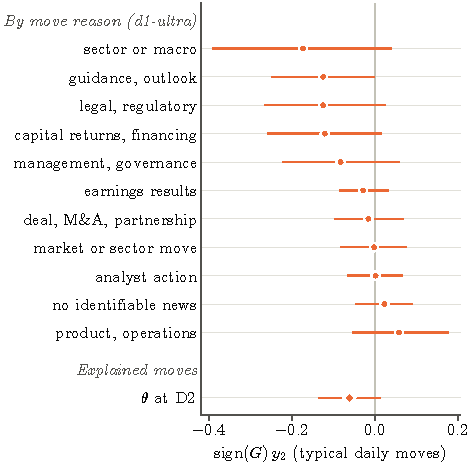
\includegraphics{figA11_persistence.pdf}
\caption{\textbf{Explained moves do not persist more.} Persistence after D2, the mean of $\mathrm{sign}(G)\,y_2$, by d1-ultra's reason for the move (95\% intervals), and $\theta$, the D2 regression of persistence on being explained: $-$0.06 (SE 0.038, p 0.946). No reason persists significantly. Days that d1-ultra judges explained are 16\% of event days and carry 41\% of their squared moves. d1-ultra is model-specific (\S{}1.3).}\label{fig:figA11_persistence}
\end{figure}

\clearpage

% t10_explanation_ladder (NA-14, from artifacts/NA-12/tables/t10_explanation_ladder.csv)
\begin{landscape}
{\scriptsize\setlength{\tabcolsep}{3pt}
\begin{longtable}{l>{\raggedright\arraybackslash}p{12em}>{\raggedright\arraybackslash}p{12em}rrrrrr}
\caption{A3.2 explanation ladder: out-of-sample share of stock-specific daily variance (z\_cc) by step}\label{tab:t10_explanation_ladder}\\
\toprule
model & cut & step & R\textsuperscript{2} & R\textsuperscript{2} CI low & R\textsuperscript{2} CI high & R\textsuperscript{2} p & increment & increment p \\
\midrule
\endfirsthead
\toprule
model & cut & step & R\textsuperscript{2} & R\textsuperscript{2} CI low & R\textsuperscript{2} CI high & R\textsuperscript{2} p & increment & increment p \\
\midrule
\endhead
\bottomrule
\endfoot
all & all & market+sector & $0.253$ & --- & --- & --- & --- & --- \\
Laya-Fin & all & ex\_\allowbreak{}ante & $0.001$ & $-2.21\times 10^{-4}$ & $0.003$ & $0.045$ & --- & --- \\
Laya-Fin & all & ex\_\allowbreak{}post & $0.002$ & $3.79\times 10^{-4}$ & $0.005$ & $0.010$ & $0.001$ & $0.010$ \\
Laya-Fin & all & ex-ante $\div$ ex-post (increment:\allowbreak{} ex-post $-$ ex-ante) & $0.532$ & --- & --- & --- & $0.001$ & --- \\
Laya-Fin & event\_\allowbreak{}days & ex\_\allowbreak{}ante & $0.004$ & $-8.47\times 10^{-4}$ & $0.008$ & $0.037$ & --- & --- \\
Laya-Fin & event\_\allowbreak{}days & ex\_\allowbreak{}post & $0.006$ & $7.29\times 10^{-5}$ & $0.012$ & $0.015$ & $0.003$ & $0.040$ \\
Laya-Fin & event\_\allowbreak{}days & ex-ante $\div$ ex-post (increment:\allowbreak{} ex-post $-$ ex-ante) & $0.588$ & --- & --- & --- & $0.003$ & --- \\
Laya-Fin & non\_\allowbreak{}event\_\allowbreak{}days & ex\_\allowbreak{}ante & $2.24\times 10^{-5}$ & $-1.23\times 10^{-4}$ & $1.72\times 10^{-4}$ & $0.389$ & --- & --- \\
Laya-Fin & tier:\allowbreak{}top100 & ex\_\allowbreak{}ante & $0.006$ & $2.45\times 10^{-5}$ & $0.013$ & $0.045$ & --- & --- \\
Laya-Fin & tier:\allowbreak{}top100 & ex\_\allowbreak{}post & $0.005$ & $0.001$ & $0.009$ & $0.009$ & $-0.001$ & $0.737$ \\
Laya-Fin & tier:\allowbreak{}top100 & ex-ante $\div$ ex-post (increment:\allowbreak{} ex-post $-$ ex-ante) & $1.203$ & --- & --- & --- & $-0.001$ & --- \\
Laya-Fin & tier:\allowbreak{}mid & ex\_\allowbreak{}ante & $-7.02\times 10^{-4}$ & $-0.003$ & $0.001$ & $0.724$ & --- & --- \\
Laya-Fin & tier:\allowbreak{}mid & ex\_\allowbreak{}post & $0.002$ & $-0.001$ & $0.004$ & $0.080$ & $0.003$ & $0.008$ \\
Laya-Fin & tier:\allowbreak{}mid & ex-ante $\div$ ex-post (increment:\allowbreak{} ex-post $-$ ex-ante) & $-0.382$ & --- & --- & --- & $0.003$ & --- \\
Laya-Fin & tier:\allowbreak{}rest & ex\_\allowbreak{}ante & $0.001$ & $-0.001$ & $0.003$ & $0.161$ & --- & --- \\
Laya-Fin & tier:\allowbreak{}rest & ex\_\allowbreak{}post & $0.002$ & $-0.001$ & $0.005$ & $0.107$ & $7.70\times 10^{-4}$ & $0.173$ \\
Laya-Fin & tier:\allowbreak{}rest & ex-ante $\div$ ex-post (increment:\allowbreak{} ex-post $-$ ex-ante) & $0.569$ & --- & --- & --- & $7.70\times 10^{-4}$ & --- \\
anchor (uninformative) & all & ex\_\allowbreak{}ante & $1.17\times 10^{-4}$ & $-1.44\times 10^{-4}$ & $3.99\times 10^{-4}$ & $0.190$ & --- & --- \\
anchor (uninformative) & all & ex\_\allowbreak{}post & $3.29\times 10^{-4}$ & $-1.31\times 10^{-4}$ & $7.59\times 10^{-4}$ & $0.072$ & $2.12\times 10^{-4}$ & $0.094$ \\
anchor (uninformative) & all & ex-ante $\div$ ex-post (increment:\allowbreak{} ex-post $-$ ex-ante) & $0.356$ & --- & --- & --- & $2.12\times 10^{-4}$ & --- \\
anchor (uninformative) & event\_\allowbreak{}days & ex\_\allowbreak{}ante & $2.71\times 10^{-4}$ & $-2.53\times 10^{-4}$ & $7.75\times 10^{-4}$ & $0.141$ & --- & --- \\
anchor (uninformative) & event\_\allowbreak{}days & ex\_\allowbreak{}post & $6.48\times 10^{-4}$ & $-4.94\times 10^{-4}$ & $0.002$ & $0.111$ & $3.77\times 10^{-4}$ & $0.140$ \\
anchor (uninformative) & event\_\allowbreak{}days & ex-ante $\div$ ex-post (increment:\allowbreak{} ex-post $-$ ex-ante) & $0.419$ & --- & --- & --- & $3.77\times 10^{-4}$ & --- \\
anchor (uninformative) & non\_\allowbreak{}event\_\allowbreak{}days & ex\_\allowbreak{}ante & $2.24\times 10^{-5}$ & $-1.23\times 10^{-4}$ & $1.72\times 10^{-4}$ & $0.389$ & --- & --- \\
anchor (uninformative) & tier:\allowbreak{}top100 & ex\_\allowbreak{}ante & $-5.45\times 10^{-4}$ & $-0.001$ & $2.51\times 10^{-4}$ & $0.914$ & --- & --- \\
anchor (uninformative) & tier:\allowbreak{}top100 & ex\_\allowbreak{}post & $-8.39\times 10^{-4}$ & $-0.002$ & $2.73\times 10^{-4}$ & $0.934$ & $-2.94\times 10^{-4}$ & $0.880$ \\
anchor (uninformative) & tier:\allowbreak{}top100 & ex-ante $\div$ ex-post (increment:\allowbreak{} ex-post $-$ ex-ante) & $0.650$ & --- & --- & --- & $-2.94\times 10^{-4}$ & --- \\
anchor (uninformative) & tier:\allowbreak{}mid & ex\_\allowbreak{}ante & $-0.001$ & $-0.002$ & $-3.61\times 10^{-4}$ & $0.996$ & --- & --- \\
anchor (uninformative) & tier:\allowbreak{}mid & ex\_\allowbreak{}post & $-7.33\times 10^{-4}$ & $-0.002$ & $5.09\times 10^{-4}$ & $0.861$ & $5.67\times 10^{-4}$ & $0.155$ \\
anchor (uninformative) & tier:\allowbreak{}mid & ex-ante $\div$ ex-post (increment:\allowbreak{} ex-post $-$ ex-ante) & $1.773$ & --- & --- & --- & $5.67\times 10^{-4}$ & --- \\
anchor (uninformative) & tier:\allowbreak{}rest & ex\_\allowbreak{}ante & $-4.62\times 10^{-5}$ & $-6.84\times 10^{-4}$ & $6.09\times 10^{-4}$ & $0.558$ & --- & --- \\
anchor (uninformative) & tier:\allowbreak{}rest & ex\_\allowbreak{}post & $2.99\times 10^{-4}$ & $-0.001$ & $0.002$ & $0.366$ & $3.45\times 10^{-4}$ & $0.314$ \\
anchor (uninformative) & tier:\allowbreak{}rest & ex-ante $\div$ ex-post (increment:\allowbreak{} ex-post $-$ ex-ante) & $-0.155$ & --- & --- & --- & $3.45\times 10^{-4}$ & --- \\
d1-ultra & all & ex\_\allowbreak{}ante & $0.003$ & $-4.80\times 10^{-4}$ & $0.006$ & $0.033$ & --- & --- \\
d1-ultra & all & ex\_\allowbreak{}post & $0.008$ & $0.004$ & $0.012$ & $<0.001$ & $0.005$ & $<0.001$ \\
d1-ultra & all & explanation & $0.158$ & $0.127$ & $0.185$ & $<0.001$ & $0.149$ & $<0.001$ \\
d1-ultra & all & ex-ante $\div$ ex-post (increment:\allowbreak{} ex-post $-$ ex-ante) & $0.348$ & --- & --- & --- & $0.005$ & --- \\
d1-ultra & event\_\allowbreak{}days & ex\_\allowbreak{}ante & $0.008$ & $0.001$ & $0.013$ & $<0.001$ & --- & --- \\
d1-ultra & event\_\allowbreak{}days & ex\_\allowbreak{}post & $0.019$ & $0.011$ & $0.026$ & $<0.001$ & $0.011$ & $<0.001$ \\
d1-ultra & event\_\allowbreak{}days & explanation & $0.375$ & $0.356$ & $0.392$ & $<0.001$ & $0.356$ & $<0.001$ \\
d1-ultra & event\_\allowbreak{}days & ex-ante $\div$ ex-post (increment:\allowbreak{} ex-post $-$ ex-ante) & $0.408$ & --- & --- & --- & $0.011$ & --- \\
d1-ultra & non\_\allowbreak{}event\_\allowbreak{}days & ex\_\allowbreak{}ante & $2.24\times 10^{-5}$ & $-1.23\times 10^{-4}$ & $1.72\times 10^{-4}$ & $0.389$ & --- & --- \\
d1-ultra & tier:\allowbreak{}top100 & ex\_\allowbreak{}ante & $0.005$ & $-1.00\times 10^{-4}$ & $0.011$ & $0.026$ & --- & --- \\
d1-ultra & tier:\allowbreak{}top100 & ex\_\allowbreak{}post & $0.009$ & $0.006$ & $0.012$ & $<0.001$ & $0.004$ & $0.005$ \\
d1-ultra & tier:\allowbreak{}top100 & explanation & $0.199$ & $0.165$ & $0.231$ & $<0.001$ & $0.190$ & $<0.001$ \\
d1-ultra & tier:\allowbreak{}top100 & ex-ante $\div$ ex-post (increment:\allowbreak{} ex-post $-$ ex-ante) & $0.602$ & --- & --- & --- & $0.004$ & --- \\
d1-ultra & tier:\allowbreak{}mid & ex\_\allowbreak{}ante & $0.002$ & $-5.55\times 10^{-4}$ & $0.004$ & $0.065$ & --- & --- \\
d1-ultra & tier:\allowbreak{}mid & ex\_\allowbreak{}post & $0.005$ & $-9.62\times 10^{-4}$ & $0.010$ & $0.048$ & $0.003$ & $0.061$ \\
d1-ultra & tier:\allowbreak{}mid & explanation & $0.156$ & $0.122$ & $0.190$ & $<0.001$ & $0.152$ & $<0.001$ \\
d1-ultra & tier:\allowbreak{}mid & ex-ante $\div$ ex-post (increment:\allowbreak{} ex-post $-$ ex-ante) & $0.369$ & --- & --- & --- & $0.003$ & --- \\
d1-ultra & tier:\allowbreak{}rest & ex\_\allowbreak{}ante & $0.003$ & $-4.55\times 10^{-5}$ & $0.006$ & $0.020$ & --- & --- \\
d1-ultra & tier:\allowbreak{}rest & ex\_\allowbreak{}post & $0.007$ & $0.002$ & $0.010$ & $<0.001$ & $0.003$ & $0.001$ \\
d1-ultra & tier:\allowbreak{}rest & explanation & $0.140$ & $0.109$ & $0.166$ & $<0.001$ & $0.133$ & $<0.001$ \\
d1-ultra & tier:\allowbreak{}rest & ex-ante $\div$ ex-post (increment:\allowbreak{} ex-post $-$ ex-ante) & $0.491$ & --- & --- & --- & $0.003$ & --- \\
d1-ultra & event\_\allowbreak{}type:\allowbreak{}analyst\_\allowbreak{}action & ex\_\allowbreak{}ante & $0.003$ & $-0.002$ & $0.009$ & $0.138$ & --- & --- \\
d1-ultra & event\_\allowbreak{}type:\allowbreak{}analyst\_\allowbreak{}action & ex\_\allowbreak{}post & $0.012$ & $0.004$ & $0.021$ & $0.007$ & $0.009$ & $<0.001$ \\
d1-ultra & event\_\allowbreak{}type:\allowbreak{}analyst\_\allowbreak{}action & explanation & $0.434$ & $0.405$ & $0.462$ & $<0.001$ & $0.422$ & $<0.001$ \\
d1-ultra & event\_\allowbreak{}type:\allowbreak{}analyst\_\allowbreak{}action & ex-ante $\div$ ex-post (increment:\allowbreak{} ex-post $-$ ex-ante) & $0.262$ & --- & --- & --- & $0.009$ & --- \\
d1-ultra & event\_\allowbreak{}type:\allowbreak{}capital\_\allowbreak{}returns\_\allowbreak{}financing & ex\_\allowbreak{}ante & $-0.034$ & $-0.086$ & $0.010$ & $0.903$ & --- & --- \\
d1-ultra & event\_\allowbreak{}type:\allowbreak{}capital\_\allowbreak{}returns\_\allowbreak{}financing & ex\_\allowbreak{}post & $-0.037$ & $-0.089$ & $0.004$ & $0.928$ & $-0.003$ & $0.641$ \\
d1-ultra & event\_\allowbreak{}type:\allowbreak{}capital\_\allowbreak{}returns\_\allowbreak{}financing & explanation & $0.317$ & $0.261$ & $0.368$ & $<0.001$ & $0.354$ & $<0.001$ \\
d1-ultra & event\_\allowbreak{}type:\allowbreak{}capital\_\allowbreak{}returns\_\allowbreak{}financing & ex-ante $\div$ ex-post (increment:\allowbreak{} ex-post $-$ ex-ante) & $0.907$ & --- & --- & --- & $-0.003$ & --- \\
d1-ultra & event\_\allowbreak{}type:\allowbreak{}deal\_\allowbreak{}ma\_\allowbreak{}partnership & ex\_\allowbreak{}ante & $-0.005$ & $-0.018$ & $0.008$ & $0.773$ & --- & --- \\
d1-ultra & event\_\allowbreak{}type:\allowbreak{}deal\_\allowbreak{}ma\_\allowbreak{}partnership & ex\_\allowbreak{}post & $0.014$ & $3.69\times 10^{-4}$ & $0.029$ & $0.026$ & $0.019$ & $<0.001$ \\
d1-ultra & event\_\allowbreak{}type:\allowbreak{}deal\_\allowbreak{}ma\_\allowbreak{}partnership & explanation & $0.380$ & $0.341$ & $0.425$ & $<0.001$ & $0.366$ & $<0.001$ \\
d1-ultra & event\_\allowbreak{}type:\allowbreak{}deal\_\allowbreak{}ma\_\allowbreak{}partnership & ex-ante $\div$ ex-post (increment:\allowbreak{} ex-post $-$ ex-ante) & $-0.338$ & --- & --- & --- & $0.019$ & --- \\
d1-ultra & event\_\allowbreak{}type:\allowbreak{}earnings\_\allowbreak{}results & ex\_\allowbreak{}ante & $0.014$ & $0.005$ & $0.022$ & $<0.001$ & --- & --- \\
d1-ultra & event\_\allowbreak{}type:\allowbreak{}earnings\_\allowbreak{}results & ex\_\allowbreak{}post & $0.026$ & $0.012$ & $0.039$ & $<0.001$ & $0.012$ & $<0.001$ \\
d1-ultra & event\_\allowbreak{}type:\allowbreak{}earnings\_\allowbreak{}results & explanation & $0.400$ & $0.377$ & $0.421$ & $<0.001$ & $0.374$ & $<0.001$ \\
d1-ultra & event\_\allowbreak{}type:\allowbreak{}earnings\_\allowbreak{}results & ex-ante $\div$ ex-post (increment:\allowbreak{} ex-post $-$ ex-ante) & $0.533$ & --- & --- & --- & $0.012$ & --- \\
d1-ultra & event\_\allowbreak{}type:\allowbreak{}guidance\_\allowbreak{}outlook & ex\_\allowbreak{}ante & $-0.035$ & $-0.072$ & $-0.006$ & $0.971$ & --- & --- \\
d1-ultra & event\_\allowbreak{}type:\allowbreak{}guidance\_\allowbreak{}outlook & ex\_\allowbreak{}post & $-0.007$ & $-0.031$ & $0.014$ & $0.717$ & $0.028$ & $0.001$ \\
d1-ultra & event\_\allowbreak{}type:\allowbreak{}guidance\_\allowbreak{}outlook & explanation & $-0.052$ & $-0.223$ & $0.030$ & $0.770$ & $-0.044$ & $0.753$ \\
d1-ultra & event\_\allowbreak{}type:\allowbreak{}guidance\_\allowbreak{}outlook & ex-ante $\div$ ex-post (increment:\allowbreak{} ex-post $-$ ex-ante) & $4.799$ & --- & --- & --- & $0.028$ & --- \\
d1-ultra & event\_\allowbreak{}type:\allowbreak{}legal\_\allowbreak{}regulatory & ex\_\allowbreak{}ante & $-0.018$ & $-0.062$ & $0.017$ & $0.807$ & --- & --- \\
d1-ultra & event\_\allowbreak{}type:\allowbreak{}legal\_\allowbreak{}regulatory & ex\_\allowbreak{}post & $-0.015$ & $-0.061$ & $0.024$ & $0.732$ & $0.004$ & $0.080$ \\
d1-ultra & event\_\allowbreak{}type:\allowbreak{}legal\_\allowbreak{}regulatory & explanation & $-1.161$ & $-4.679$ & $0.416$ & $0.769$ & $-1.146$ & $0.766$ \\
d1-ultra & event\_\allowbreak{}type:\allowbreak{}legal\_\allowbreak{}regulatory & ex-ante $\div$ ex-post (increment:\allowbreak{} ex-post $-$ ex-ante) & $1.252$ & --- & --- & --- & $0.004$ & --- \\
d1-ultra & event\_\allowbreak{}type:\allowbreak{}management\_\allowbreak{}governance & ex\_\allowbreak{}ante & $0.006$ & $-0.008$ & $0.017$ & $0.164$ & --- & --- \\
d1-ultra & event\_\allowbreak{}type:\allowbreak{}management\_\allowbreak{}governance & ex\_\allowbreak{}post & $0.002$ & $-0.002$ & $0.006$ & $0.153$ & $-0.003$ & $0.737$ \\
d1-ultra & event\_\allowbreak{}type:\allowbreak{}management\_\allowbreak{}governance & explanation & $0.170$ & $0.099$ & $0.249$ & $<0.001$ & $0.168$ & $<0.001$ \\
d1-ultra & event\_\allowbreak{}type:\allowbreak{}management\_\allowbreak{}governance & ex-ante $\div$ ex-post (increment:\allowbreak{} ex-post $-$ ex-ante) & $2.551$ & --- & --- & --- & $-0.003$ & --- \\
d1-ultra & event\_\allowbreak{}type:\allowbreak{}other & ex\_\allowbreak{}ante & $-0.004$ & $-0.008$ & $-4.27\times 10^{-4}$ & $0.984$ & --- & --- \\
d1-ultra & event\_\allowbreak{}type:\allowbreak{}other & ex\_\allowbreak{}post & $-0.004$ & $-0.012$ & $0.004$ & $0.856$ & $-4.85\times 10^{-5}$ & $0.498$ \\
d1-ultra & event\_\allowbreak{}type:\allowbreak{}other & explanation & $0.194$ & $0.166$ & $0.230$ & $<0.001$ & $0.198$ & $<0.001$ \\
d1-ultra & event\_\allowbreak{}type:\allowbreak{}other & ex-ante $\div$ ex-post (increment:\allowbreak{} ex-post $-$ ex-ante) & $0.988$ & --- & --- & --- & $-4.85\times 10^{-5}$ & --- \\
d1-ultra & event\_\allowbreak{}type:\allowbreak{}product\_\allowbreak{}operations & ex\_\allowbreak{}ante & $-0.003$ & $-0.010$ & $0.003$ & $0.843$ & --- & --- \\
d1-ultra & event\_\allowbreak{}type:\allowbreak{}product\_\allowbreak{}operations & ex\_\allowbreak{}post & $-0.003$ & $-0.010$ & $0.003$ & $0.823$ & $2.80\times 10^{-4}$ & $0.013$ \\
d1-ultra & event\_\allowbreak{}type:\allowbreak{}product\_\allowbreak{}operations & explanation & $0.355$ & $0.308$ & $0.396$ & $<0.001$ & $0.359$ & $<0.001$ \\
d1-ultra & event\_\allowbreak{}type:\allowbreak{}product\_\allowbreak{}operations & ex-ante $\div$ ex-post (increment:\allowbreak{} ex-post $-$ ex-ante) & $1.090$ & --- & --- & --- & $2.80\times 10^{-4}$ & --- \\
d1-ultra & event\_\allowbreak{}type:\allowbreak{}sector\_\allowbreak{}or\_\allowbreak{}macro & ex\_\allowbreak{}ante & $-0.003$ & $-0.008$ & $0.002$ & $0.851$ & --- & --- \\
d1-ultra & event\_\allowbreak{}type:\allowbreak{}sector\_\allowbreak{}or\_\allowbreak{}macro & ex\_\allowbreak{}post & $0.031$ & $-0.009$ & $0.058$ & $0.009$ & $0.033$ & $0.003$ \\
d1-ultra & event\_\allowbreak{}type:\allowbreak{}sector\_\allowbreak{}or\_\allowbreak{}macro & explanation & $0.349$ & $0.145$ & $0.505$ & $<0.001$ & $0.318$ & $<0.001$ \\
d1-ultra & event\_\allowbreak{}type:\allowbreak{}sector\_\allowbreak{}or\_\allowbreak{}macro & ex-ante $\div$ ex-post (increment:\allowbreak{} ex-post $-$ ex-ante) & $-0.088$ & --- & --- & --- & $0.033$ & --- \\
\end{longtable}
\par\smallskip{\footnotesize\raggedright Ridge fit on val-B, $\lambda$ on val-A, evaluated on test (\S{}11.5); news features are 0 on days without an event. Selected columns; every cell is in t10\_explanation\_ladder.csv. The anchor's readings are uninformative (near-constant outputs: NA-11 REPORT \S{}7.1 item 4); its rows are reported, not read as nulls.\par}
}
\end{landscape}


\clearpage

% t11_explanation_share_theta (NA-14, from artifacts/NA-12/tables/t11_explanation_share_theta.csv)
\begin{table*}[tbp]
\centering\small
\caption{A3.3--A3.5 (d1-ultra, model-specific): explained share, $\theta$, persistence by reason, the market}\label{tab:t11_explanation_share_theta}
\begin{adjustbox}{max width=\textwidth}
\begin{tabular}{>{\raggedright\arraybackslash}p{12em}rrrrrrrrl}
\toprule
item & value & events share & n & variance share & SE & p & CI low & CI high & available \\
\midrule
share of $\Sigma$z\_\allowbreak{}cc\textsuperscript{2} on days judged explained (X $>$= 0.5) & $0.410$ & $0.156$ & $18{,}291$ & --- & --- & --- & --- & --- & --- \\
explained share, mid & $0.421$ & --- & --- & --- & --- & --- & --- & --- & --- \\
explained share, rest & $0.401$ & --- & --- & --- & --- & --- & --- & --- & --- \\
explained share, top100 & $0.413$ & --- & --- & --- & --- & --- & --- & --- & --- \\
explained share, reason analyst\_\allowbreak{}action & $0.342$ & --- & $3{,}269$ & $0.103$ & --- & --- & --- & --- & --- \\
explained share, reason capital\_\allowbreak{}returns\_\allowbreak{}financing & $0.278$ & --- & $410$ & $0.013$ & --- & --- & --- & --- & --- \\
explained share, reason deal\_\allowbreak{}ma\_\allowbreak{}partnership & $0.336$ & --- & $1{,}192$ & $0.050$ & --- & --- & --- & --- & --- \\
explained share, reason earnings\_\allowbreak{}results & $0.536$ & --- & $4{,}592$ & $0.570$ & --- & --- & --- & --- & --- \\
explained share, reason guidance\_\allowbreak{}outlook & $0.500$ & --- & $622$ & $0.043$ & --- & --- & --- & --- & --- \\
explained share, reason legal\_\allowbreak{}regulatory & $0.313$ & --- & $423$ & $0.015$ & --- & --- & --- & --- & --- \\
explained share, reason management\_\allowbreak{}governance & $0.071$ & --- & $263$ & $0.009$ & --- & --- & --- & --- & --- \\
explained share, reason market\_\allowbreak{}or\_\allowbreak{}sector\_\allowbreak{}move & $0.036$ & --- & $2{,}113$ & $0.011$ & --- & --- & --- & --- & --- \\
explained share, reason no\_\allowbreak{}identifiable\_\allowbreak{}news & $0.021$ & --- & $4{,}387$ & $0.144$ & --- & --- & --- & --- & --- \\
explained share, reason product\_\allowbreak{}operations & $0.338$ & --- & $782$ & $0.029$ & --- & --- & --- & --- & --- \\
explained share, reason sector\_\allowbreak{}or\_\allowbreak{}macro & $0.622$ & --- & $238$ & $0.013$ & --- & --- & --- & --- & --- \\
$\theta$ at D2 (explanation $\to$ persistence) & $-0.062$ & --- & $17{,}188$ & --- & $0.038$ & $0.946$ & --- & --- & --- \\
$\theta$ at D1 (explanation $\to$ persistence) & $-0.040$ & --- & $13{,}203$ & --- & $0.036$ & $0.868$ & --- & --- & --- \\
mean sign(G)$\cdot$y2, reason analyst\_\allowbreak{}action & $0.001$ & --- & $3{,}159$ & --- & --- & $0.491$ & $-0.065$ & $0.067$ & --- \\
mean sign(G)$\cdot$y2, reason capital\_\allowbreak{}returns\_\allowbreak{}financing & $-0.121$ & --- & $392$ & --- & --- & $0.960$ & $-0.259$ & $0.016$ & --- \\
mean sign(G)$\cdot$y2, reason deal\_\allowbreak{}ma\_\allowbreak{}partnership & $-0.016$ & --- & $1{,}136$ & --- & --- & $0.646$ & $-0.098$ & $0.069$ & --- \\
mean sign(G)$\cdot$y2, reason earnings\_\allowbreak{}results & $-0.028$ & --- & $4{,}204$ & --- & --- & $0.842$ & $-0.086$ & $0.032$ & --- \\
mean sign(G)$\cdot$y2, reason guidance\_\allowbreak{}outlook & $-0.125$ & --- & $572$ & --- & --- & $0.976$ & $-0.250$ & $-7.08\times 10^{-4}$ & --- \\
mean sign(G)$\cdot$y2, reason legal\_\allowbreak{}regulatory & $-0.125$ & --- & $408$ & --- & --- & $0.956$ & $-0.267$ & $0.025$ & --- \\
mean sign(G)$\cdot$y2, reason management\_\allowbreak{}governance & $-0.083$ & --- & $254$ & --- & --- & $0.877$ & $-0.223$ & $0.059$ & --- \\
mean sign(G)$\cdot$y2, reason market\_\allowbreak{}or\_\allowbreak{}sector\_\allowbreak{}move & $-0.002$ & --- & $1{,}986$ & --- & --- & $0.540$ & $-0.083$ & $0.076$ & --- \\
mean sign(G)$\cdot$y2, reason no\_\allowbreak{}identifiable\_\allowbreak{}news & $0.023$ & --- & $4{,}091$ & --- & --- & $0.260$ & $-0.048$ & $0.091$ & --- \\
mean sign(G)$\cdot$y2, reason product\_\allowbreak{}operations & $0.058$ & --- & $758$ & --- & --- & $0.168$ & $-0.055$ & $0.177$ & --- \\
mean sign(G)$\cdot$y2, reason sector\_\allowbreak{}or\_\allowbreak{}macro & $-0.173$ & --- & $228$ & --- & --- & $0.945$ & $-0.390$ & $0.040$ & --- \\
A3.5 market replication, OOS R\textsuperscript{2} of SPY's r\_\allowbreak{}cc (exploratory) & $0.021$ & --- & $144$ & --- & --- & $0.309$ & $-0.066$ & $0.107$ & yes \\
\bottomrule
\end{tabular}
\end{adjustbox}
\end{table*}


\clearpage

% t12_question_battery: tab:a-question-battery (NA-14 figures.latex, from artifacts/NA-14/tables/t12_question_battery.csv)
\begin{landscape}
\begingroup
\footnotesize
\setlength{\tabcolsep}{4pt}
\begin{longtable}{@{}>{\raggedright\arraybackslash}p{3.5in}S[table-format=-3.3]S[table-format=1.3]S[table-format=-1.3]S[table-format=1.3]S[table-format=-2.3]S[table-format=-1.3]S[table-format=1.3, table-space-text-pre={$<$}]S[table-format=1.4]S[table-format=1.3]S[table-format=5.0]@{}}
\caption{Question battery v2: mechanism cuts, horizon validity and width.}\label{tab:a-question-battery} \\
\toprule
Model, analysis, label, level & {$b$} & {$p_b$} & {$c$} & {$p_c$} & {$\kappa_{t+20}$} & {$\rho$} & {$p$} & {$\Delta R^2$} & {Agreement} & {Events} \\
\midrule
\endfirsthead
\multicolumn{11}{@{}l}{\textit{Table \ref{tab:a-question-battery}, continued}} \\
\toprule
Model, analysis, label, level & {$b$} & {$p_b$} & {$c$} & {$p_c$} & {$\kappa_{t+20}$} & {$\rho$} & {$p$} & {$\Delta R^2$} & {Agreement} & {Events} \\
\midrule
\endhead
\midrule
\multicolumn{11}{r@{}}{\textit{continued on the next page}} \\
\endfoot
\bottomrule
\endlastfoot
Laya-Fin, H2 at D2, vendor event type, analyst action & 0.365 & 0.336 & 0.041 & 0.895 & {---} & {---} & {---} & {---} & {---} & 1734 \\
Laya-Fin, H2 at D2, vendor event type, capital returns & -4.884 & 0.814 & 0.100 & 0.692 & {---} & {---} & {---} & {---} & {---} & 343 \\
Laya-Fin, H2 at D2, vendor event type, competition & -3.675 & 0.680 & -0.196 & 0.192 & {---} & {---} & {---} & {---} & {---} & 215 \\
Laya-Fin, H2 at D2, vendor event type, earnings results & -0.028 & 0.570 & -0.021 & 0.041 & {---} & {---} & {---} & {---} & {---} & 10828 \\
Laya-Fin, H2 at D2, vendor event type, financing dilution & {---} & {---} & {---} & {---} & {---} & {---} & {---} & {---} & {---} & {---} \\
Laya-Fin, H2 at D2, vendor event type, guidance outlook & 0.050 & 0.475 & 0.035 & 0.779 & {---} & {---} & {---} & {---} & {---} & 1549 \\
Laya-Fin, H2 at D2, vendor event type, insider ownership & -3.853 & 0.825 & 0.121 & 0.796 & {---} & {---} & {---} & {---} & {---} & 254 \\
Laya-Fin, H2 at D2, vendor event type, leadership governance & -0.371 & 0.518 & -0.101 & 0.392 & {---} & {---} & {---} & {---} & {---} & 160 \\
Laya-Fin, H2 at D2, vendor event type, legal regulatory & -1.938 & 0.619 & 0.270 & 0.798 & {---} & {---} & {---} & {---} & {---} & 117 \\
Laya-Fin, H2 at D2, vendor event type, M\&A deal & -12.871 & 0.664 & -0.224 & 0.363 & {---} & {---} & {---} & {---} & {---} & 141 \\
Laya-Fin, H2 at D2, vendor event type, macro sector & -1.326 & 0.676 & 0.057 & 0.680 & {---} & {---} & {---} & {---} & {---} & 516 \\
Laya-Fin, H2 at D2, vendor event type, operations supply & 2.450 & 0.234 & -0.132 & 0.276 & {---} & {---} & {---} & {---} & {---} & 300 \\
Laya-Fin, H2 at D2, vendor event type, other corporate & -8.550 & 0.913 & -0.160 & 0.091 & {---} & {---} & {---} & {---} & {---} & 233 \\
Laya-Fin, H2 at D2, vendor event type, partnership customer & 0.218 & 0.460 & -0.061 & 0.413 & {---} & {---} & {---} & {---} & {---} & 342 \\
Laya-Fin, H2 at D2, vendor event type, product launch & 2.262 & 0.284 & -0.154 & 0.111 & {---} & {---} & {---} & {---} & {---} & 420 \\
Laya-Fin, H2 at D2, vendor quantified flag, no & -0.156 & 0.601 & -0.037 & 0.115 & {---} & {---} & {---} & {---} & {---} & 2158 \\
Laya-Fin, H2 at D2, vendor quantified flag, yes & -0.015 & 0.538 & -0.013 & 0.145 & {---} & {---} & {---} & {---} & {---} & 15030 \\
Laya-Fin, ladder, vendor event type, analyst action & {---} & {---} & {---} & {---} & 2.622 & {---} & {---} & {---} & {---} & 1049 \\
Laya-Fin, ladder, vendor event type, capital returns & {---} & {---} & {---} & {---} & -2.533 & {---} & {---} & {---} & {---} & 233 \\
Laya-Fin, ladder, vendor event type, competition & {---} & {---} & {---} & {---} & 6.758 & {---} & {---} & {---} & {---} & 91 \\
Laya-Fin, ladder, vendor event type, earnings results & {---} & {---} & {---} & {---} & 0.259 & {---} & {---} & {---} & {---} & 7453 \\
Laya-Fin, ladder, vendor event type, guidance outlook & {---} & {---} & {---} & {---} & 0.980 & {---} & {---} & {---} & {---} & 852 \\
Laya-Fin, ladder, vendor event type, insider ownership & {---} & {---} & {---} & {---} & 1.171 & {---} & {---} & {---} & {---} & 176 \\
Laya-Fin, ladder, vendor event type, leadership governance & {---} & {---} & {---} & {---} & -1.746 & {---} & {---} & {---} & {---} & 112 \\
Laya-Fin, ladder, vendor event type, legal regulatory & {---} & {---} & {---} & {---} & 27.043 & {---} & {---} & {---} & {---} & 75 \\
Laya-Fin, ladder, vendor event type, M\&A deal & {---} & {---} & {---} & {---} & 2.751 & {---} & {---} & {---} & {---} & 88 \\
Laya-Fin, ladder, vendor event type, macro sector & {---} & {---} & {---} & {---} & 0.430 & {---} & {---} & {---} & {---} & 245 \\
Laya-Fin, ladder, vendor event type, operations supply & {---} & {---} & {---} & {---} & 9.130 & {---} & {---} & {---} & {---} & 191 \\
Laya-Fin, ladder, vendor event type, other corporate & {---} & {---} & {---} & {---} & -10.376 & {---} & {---} & {---} & {---} & 153 \\
Laya-Fin, ladder, vendor event type, partnership customer & {---} & {---} & {---} & {---} & 2.230 & {---} & {---} & {---} & {---} & 216 \\
Laya-Fin, ladder, vendor event type, product launch & {---} & {---} & {---} & {---} & 6.641 & {---} & {---} & {---} & {---} & 244 \\
Laya-Fin, ladder, vendor quantified flag, no & {---} & {---} & {---} & {---} & 0.044 & {---} & {---} & {---} & {---} & 1310 \\
Laya-Fin, ladder, vendor quantified flag, yes & {---} & {---} & {---} & {---} & 0.248 & {---} & {---} & {---} & {---} & 9891 \\
anchor, H2 at D2, vendor event type, analyst action & 17.803 & 0.129 & 0.043 & 0.901 & {---} & {---} & {---} & {---} & {---} & 1734 \\
anchor, H2 at D2, vendor event type, capital returns & -66.994 & 0.553 & 0.105 & 0.711 & {---} & {---} & {---} & {---} & {---} & 343 \\
anchor, H2 at D2, vendor event type, competition & 577.271 & 0.324 & -0.175 & 0.246 & {---} & {---} & {---} & {---} & {---} & 215 \\
anchor, H2 at D2, vendor event type, earnings results & 0.253 & 0.433 & -0.021 & 0.043 & {---} & {---} & {---} & {---} & {---} & 10828 \\
anchor, H2 at D2, vendor event type, financing dilution & {---} & {---} & {---} & {---} & {---} & {---} & {---} & {---} & {---} & {---} \\
anchor, H2 at D2, vendor event type, guidance outlook & 1.477 & 0.443 & 0.035 & 0.780 & {---} & {---} & {---} & {---} & {---} & 1549 \\
anchor, H2 at D2, vendor event type, insider ownership & 111.904 & 0.445 & 0.152 & 0.830 & {---} & {---} & {---} & {---} & {---} & 254 \\
anchor, H2 at D2, vendor event type, leadership governance & 196.719 & 0.419 & -0.093 & 0.407 & {---} & {---} & {---} & {---} & {---} & 160 \\
anchor, H2 at D2, vendor event type, legal regulatory & 539.007 & 0.326 & 0.227 & 0.745 & {---} & {---} & {---} & {---} & {---} & 117 \\
anchor, H2 at D2, vendor event type, M\&A deal & 86.356 & 0.489 & -0.218 & 0.357 & {---} & {---} & {---} & {---} & {---} & 141 \\
anchor, H2 at D2, vendor event type, macro sector & -9.396 & 0.680 & 0.049 & 0.657 & {---} & {---} & {---} & {---} & {---} & 516 \\
anchor, H2 at D2, vendor event type, operations supply & 114.038 & 0.424 & -0.118 & 0.295 & {---} & {---} & {---} & {---} & {---} & 300 \\
anchor, H2 at D2, vendor event type, other corporate & 594.767 & 0.260 & -0.101 & 0.142 & {---} & {---} & {---} & {---} & {---} & 233 \\
anchor, H2 at D2, vendor event type, partnership customer & 452.483 & 0.266 & -0.045 & 0.432 & {---} & {---} & {---} & {---} & {---} & 342 \\
anchor, H2 at D2, vendor event type, product launch & -326.856 & 0.838 & -0.146 & 0.124 & {---} & {---} & {---} & {---} & {---} & 420 \\
anchor, H2 at D2, vendor quantified flag, no & -7.930 & 0.746 & -0.036 & 0.122 & {---} & {---} & {---} & {---} & {---} & 2158 \\
anchor, H2 at D2, vendor quantified flag, yes & 1.112 & 0.205 & -0.013 & 0.149 & {---} & {---} & {---} & {---} & {---} & 15030 \\
anchor, ladder, vendor event type, analyst action & {---} & {---} & {---} & {---} & 5.034 & {---} & {---} & {---} & {---} & 1049 \\
anchor, ladder, vendor event type, capital returns & {---} & {---} & {---} & {---} & -10.957 & {---} & {---} & {---} & {---} & 233 \\
anchor, ladder, vendor event type, competition & {---} & {---} & {---} & {---} & 14.767 & {---} & {---} & {---} & {---} & 91 \\
anchor, ladder, vendor event type, earnings results & {---} & {---} & {---} & {---} & 0.017 & {---} & {---} & {---} & {---} & 7453 \\
anchor, ladder, vendor event type, guidance outlook & {---} & {---} & {---} & {---} & 0.448 & {---} & {---} & {---} & {---} & 852 \\
anchor, ladder, vendor event type, insider ownership & {---} & {---} & {---} & {---} & 6.976 & {---} & {---} & {---} & {---} & 176 \\
anchor, ladder, vendor event type, leadership governance & {---} & {---} & {---} & {---} & 13.068 & {---} & {---} & {---} & {---} & 112 \\
anchor, ladder, vendor event type, legal regulatory & {---} & {---} & {---} & {---} & -3.293 & {---} & {---} & {---} & {---} & 75 \\
anchor, ladder, vendor event type, M\&A deal & {---} & {---} & {---} & {---} & 63.554 & {---} & {---} & {---} & {---} & 88 \\
anchor, ladder, vendor event type, macro sector & {---} & {---} & {---} & {---} & 5.512 & {---} & {---} & {---} & {---} & 245 \\
anchor, ladder, vendor event type, operations supply & {---} & {---} & {---} & {---} & 24.972 & {---} & {---} & {---} & {---} & 191 \\
anchor, ladder, vendor event type, other corporate & {---} & {---} & {---} & {---} & -50.410 & {---} & {---} & {---} & {---} & 153 \\
anchor, ladder, vendor event type, partnership customer & {---} & {---} & {---} & {---} & -1.182 & {---} & {---} & {---} & {---} & 216 \\
anchor, ladder, vendor event type, product launch & {---} & {---} & {---} & {---} & 16.391 & {---} & {---} & {---} & {---} & 244 \\
anchor, ladder, vendor quantified flag, no & {---} & {---} & {---} & {---} & -0.726 & {---} & {---} & {---} & {---} & 1310 \\
anchor, ladder, vendor quantified flag, yes & {---} & {---} & {---} & {---} & 0.077 & {---} & {---} & {---} & {---} & 9891 \\
d1-ultra, H2 at D2, own event type (Call A, same-day news), analyst action & -0.132 & 0.987 & 0.006 & 0.593 & {---} & {---} & {---} & {---} & {---} & 3474 \\
d1-ultra, H2 at D2, own event type (Call A, same-day news), capital returns financing & -0.403 & 0.931 & 0.009 & 0.541 & {---} & {---} & {---} & {---} & {---} & 609 \\
d1-ultra, H2 at D2, own event type (Call A, same-day news), deal, M\&A, partnership & 0.047 & 0.360 & -0.049 & 0.177 & {---} & {---} & {---} & {---} & {---} & 1212 \\
d1-ultra, H2 at D2, own event type (Call A, same-day news), earnings results & -0.088 & 0.991 & -0.020 & 0.061 & {---} & {---} & {---} & {---} & {---} & 6501 \\
d1-ultra, H2 at D2, own event type (Call A, same-day news), guidance outlook & 0.032 & 0.437 & 0.029 & 0.633 & {---} & {---} & {---} & {---} & {---} & 463 \\
d1-ultra, H2 at D2, own event type (Call A, same-day news), legal regulatory & -0.138 & 0.757 & -0.014 & 0.468 & {---} & {---} & {---} & {---} & {---} & 443 \\
d1-ultra, H2 at D2, own event type (Call A, same-day news), management governance & 0.036 & 0.468 & -0.055 & 0.383 & {---} & {---} & {---} & {---} & {---} & 306 \\
d1-ultra, H2 at D2, own event type (Call A, same-day news), other & 0.003 & 0.490 & 0.006 & 0.567 & {---} & {---} & {---} & {---} & {---} & 2810 \\
d1-ultra, H2 at D2, own event type (Call A, same-day news), product operations & 0.133 & 0.243 & 0.003 & 0.517 & {---} & {---} & {---} & {---} & {---} & 1039 \\
d1-ultra, H2 at D2, own event type (Call A, same-day news), sector or macro & -0.230 & 0.662 & 0.171 & 0.867 & {---} & {---} & {---} & {---} & {---} & 331 \\
d1-ultra, H2 at D2, own quantified flag (Call A, same-day news), narrative & -0.066 & 0.950 & -0.008 & 0.322 & {---} & {---} & {---} & {---} & {---} & 11665 \\
d1-ultra, H2 at D2, own quantified flag (Call A, same-day news), numbers & -0.061 & 0.912 & -0.010 & 0.219 & {---} & {---} & {---} & {---} & {---} & 5523 \\
d1-ultra, H2 at D2, vendor event type, analyst action & -0.095 & 0.885 & 0.048 & 0.923 & {---} & {---} & {---} & {---} & {---} & 1734 \\
d1-ultra, H2 at D2, vendor event type, capital returns & -0.650 & 0.939 & 0.100 & 0.697 & {---} & {---} & {---} & {---} & {---} & 343 \\
d1-ultra, H2 at D2, vendor event type, competition & -0.164 & 0.598 & -0.162 & 0.269 & {---} & {---} & {---} & {---} & {---} & 215 \\
d1-ultra, H2 at D2, vendor event type, earnings results & -0.077 & 0.982 & -0.018 & 0.072 & {---} & {---} & {---} & {---} & {---} & 10828 \\
d1-ultra, H2 at D2, vendor event type, financing dilution & {---} & {---} & {---} & {---} & {---} & {---} & {---} & {---} & {---} & {---} \\
d1-ultra, H2 at D2, vendor event type, guidance outlook & 0.012 & 0.467 & 0.035 & 0.777 & {---} & {---} & {---} & {---} & {---} & 1549 \\
d1-ultra, H2 at D2, vendor event type, insider ownership & -0.201 & 0.656 & 0.149 & 0.844 & {---} & {---} & {---} & {---} & {---} & 254 \\
d1-ultra, H2 at D2, vendor event type, leadership governance & -0.513 & 0.776 & -0.080 & 0.409 & {---} & {---} & {---} & {---} & {---} & 160 \\
d1-ultra, H2 at D2, vendor event type, legal regulatory & 0.233 & 0.315 & 0.321 & 0.850 & {---} & {---} & {---} & {---} & {---} & 117 \\
d1-ultra, H2 at D2, vendor event type, M\&A deal & -0.100 & 0.525 & -0.210 & 0.376 & {---} & {---} & {---} & {---} & {---} & 141 \\
d1-ultra, H2 at D2, vendor event type, macro sector & -0.076 & 0.604 & 0.052 & 0.669 & {---} & {---} & {---} & {---} & {---} & 516 \\
d1-ultra, H2 at D2, vendor event type, operations supply & 0.147 & 0.326 & -0.127 & 0.288 & {---} & {---} & {---} & {---} & {---} & 300 \\
d1-ultra, H2 at D2, vendor event type, other corporate & -0.446 & 0.693 & -0.110 & 0.146 & {---} & {---} & {---} & {---} & {---} & 233 \\
d1-ultra, H2 at D2, vendor event type, partnership customer & -0.110 & 0.589 & -0.050 & 0.432 & {---} & {---} & {---} & {---} & {---} & 342 \\
d1-ultra, H2 at D2, vendor event type, product launch & 0.291 & 0.183 & -0.157 & 0.107 & {---} & {---} & {---} & {---} & {---} & 420 \\
d1-ultra, H2 at D2, vendor quantified flag, no & -0.001 & 0.503 & -0.038 & 0.116 & {---} & {---} & {---} & {---} & {---} & 2158 \\
d1-ultra, H2 at D2, vendor quantified flag, yes & -0.084 & 0.994 & -0.009 & 0.227 & {---} & {---} & {---} & {---} & {---} & 15030 \\
d1-ultra, ladder, own event type (Call A, pre-open news), analyst action & {---} & {---} & {---} & {---} & 0.254 & {---} & {---} & {---} & {---} & 1804 \\
d1-ultra, ladder, own event type (Call A, pre-open news), capital returns financing & {---} & {---} & {---} & {---} & -1.389 & {---} & {---} & {---} & {---} & 397 \\
d1-ultra, ladder, own event type (Call A, pre-open news), deal, M\&A, partnership & {---} & {---} & {---} & {---} & -1.086 & {---} & {---} & {---} & {---} & 694 \\
d1-ultra, ladder, own event type (Call A, pre-open news), earnings results & {---} & {---} & {---} & {---} & 0.596 & {---} & {---} & {---} & {---} & 4966 \\
d1-ultra, ladder, own event type (Call A, pre-open news), guidance outlook & {---} & {---} & {---} & {---} & 2.117 & {---} & {---} & {---} & {---} & 315 \\
d1-ultra, ladder, own event type (Call A, pre-open news), legal regulatory & {---} & {---} & {---} & {---} & -1.178 & {---} & {---} & {---} & {---} & 233 \\
d1-ultra, ladder, own event type (Call A, pre-open news), management governance & {---} & {---} & {---} & {---} & 0.206 & {---} & {---} & {---} & {---} & 200 \\
d1-ultra, ladder, own event type (Call A, pre-open news), other & {---} & {---} & {---} & {---} & 1.346 & {---} & {---} & {---} & {---} & 1818 \\
d1-ultra, ladder, own event type (Call A, pre-open news), product operations & {---} & {---} & {---} & {---} & -0.150 & {---} & {---} & {---} & {---} & 569 \\
d1-ultra, ladder, own event type (Call A, pre-open news), sector or macro & {---} & {---} & {---} & {---} & 16.931 & {---} & {---} & {---} & {---} & 205 \\
d1-ultra, ladder, own quantified flag (Call A, pre-open news), narrative & {---} & {---} & {---} & {---} & -0.039 & {---} & {---} & {---} & {---} & 7450 \\
d1-ultra, ladder, own quantified flag (Call A, pre-open news), numbers & {---} & {---} & {---} & {---} & 0.784 & {---} & {---} & {---} & {---} & 3751 \\
d1-ultra, ladder, vendor event type, analyst action & {---} & {---} & {---} & {---} & 0.940 & {---} & {---} & {---} & {---} & 1049 \\
d1-ultra, ladder, vendor event type, capital returns & {---} & {---} & {---} & {---} & 0.118 & {---} & {---} & {---} & {---} & 233 \\
d1-ultra, ladder, vendor event type, competition & {---} & {---} & {---} & {---} & 0.536 & {---} & {---} & {---} & {---} & 91 \\
d1-ultra, ladder, vendor event type, earnings results & {---} & {---} & {---} & {---} & 0.446 & {---} & {---} & {---} & {---} & 7453 \\
d1-ultra, ladder, vendor event type, guidance outlook & {---} & {---} & {---} & {---} & 0.329 & {---} & {---} & {---} & {---} & 852 \\
d1-ultra, ladder, vendor event type, insider ownership & {---} & {---} & {---} & {---} & 2.799 & {---} & {---} & {---} & {---} & 176 \\
d1-ultra, ladder, vendor event type, leadership governance & {---} & {---} & {---} & {---} & 1.937 & {---} & {---} & {---} & {---} & 112 \\
d1-ultra, ladder, vendor event type, legal regulatory & {---} & {---} & {---} & {---} & -7.286 & {---} & {---} & {---} & {---} & 75 \\
d1-ultra, ladder, vendor event type, M\&A deal & {---} & {---} & {---} & {---} & -4.585 & {---} & {---} & {---} & {---} & 88 \\
d1-ultra, ladder, vendor event type, macro sector & {---} & {---} & {---} & {---} & 3.215 & {---} & {---} & {---} & {---} & 245 \\
d1-ultra, ladder, vendor event type, operations supply & {---} & {---} & {---} & {---} & 2.668 & {---} & {---} & {---} & {---} & 191 \\
d1-ultra, ladder, vendor event type, other corporate & {---} & {---} & {---} & {---} & -4.239 & {---} & {---} & {---} & {---} & 153 \\
d1-ultra, ladder, vendor event type, partnership customer & {---} & {---} & {---} & {---} & -1.230 & {---} & {---} & {---} & {---} & 216 \\
d1-ultra, ladder, vendor event type, product launch & {---} & {---} & {---} & {---} & 0.196 & {---} & {---} & {---} & {---} & 244 \\
d1-ultra, ladder, vendor quantified flag, no & {---} & {---} & {---} & {---} & 0.264 & {---} & {---} & {---} & {---} & 1310 \\
d1-ultra, ladder, vendor quantified flag, yes & {---} & {---} & {---} & {---} & 0.390 & {---} & {---} & {---} & {---} & 9891 \\
d1-ultra, horizon validity: Spearman($H$, share of the $t{+}20$ move by $C_t$) & {---} & {---} & {---} & {---} & {---} & -0.068 & {$<$}0.001 & {---} & {---} & 9683 \\
d1-ultra, H4 width: $\Delta R^2$ of the uncertainty score and $P$(no material effect) & {---} & {---} & {---} & {---} & {---} & {---} & 0.245 & 0.0001 & {---} & {---} \\
d1-ultra, reading validity (NA-06, val-A): credibility & {---} & {---} & {---} & {---} & {---} & {---} & {---} & {---} & 0.990 & 500 \\
d1-ultra, reading validity (NA-06, val-A): event type & {---} & {---} & {---} & {---} & {---} & {---} & {---} & {---} & 0.572 & 500 \\
d1-ultra, reading validity (NA-06, val-A): event type vs raw tag & {---} & {---} & {---} & {---} & {---} & {---} & {---} & {---} & 0.454 & 500 \\
d1-ultra, reading validity (NA-06, val-A): quantified & {---} & {---} & {---} & {---} & {---} & {---} & {---} & {---} & 0.494 & 500 \\
d1-ultra, reading validity (NA-06, val-A): scheduled & {---} & {---} & {---} & {---} & {---} & {---} & {---} & {---} & 0.552 & 500 \\
\end{longtable}
\endgroup
\vspace{-0.5\baselineskip}
{\footnotesize\raggedright
---: the source table has no value for the row; the statistic does not apply to it or was not computed.\par
Reading validity: the share of the 500 val-A events on which d1-ultra's answer agrees with the vendor's tag (event type, the raw tag, quantified; the rumor tag for credibility) or with the earnings calendar (scheduled).\par
The anchor's readings are uninformative (near-constant outputs after one epoch); its rows are reported, not read as nulls.\par
The API models fail the pre-registered contamination screens, so their results are model-specific.\par
}
\end{landscape}


\clearpage

\section{Economic significance}

\begin{figure}[htbp]
\centering
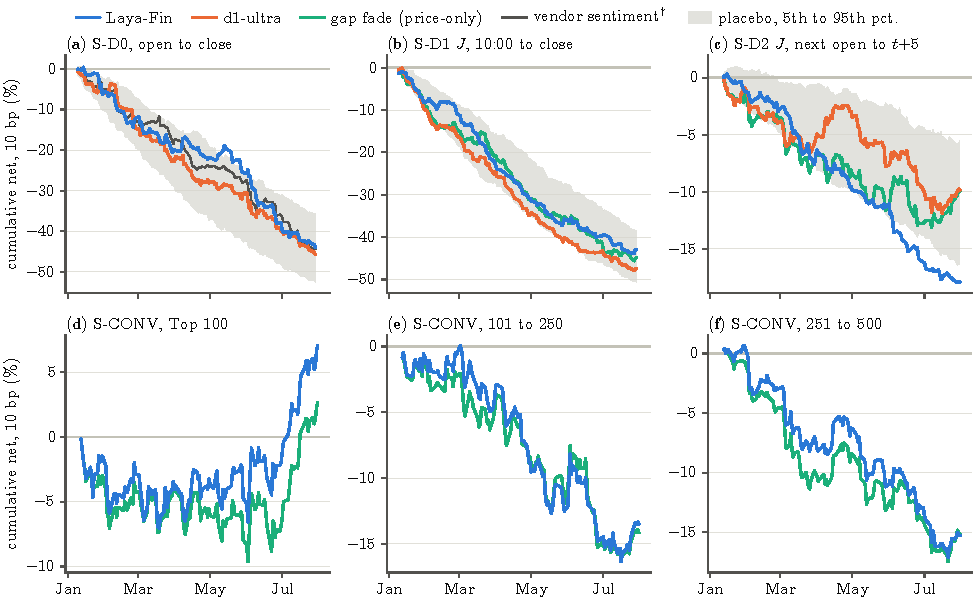
\includegraphics{figA12_strategy_paths.pdf}
\caption{\textbf{The other books, and S-CONV by tier.} Cumulative net returns at 10 bp per side over the test period (NA-13). (a) S-D0 from the open to the close, with vendor sentiment ($\dagger$: a possibly look-ahead-contaminated upper bound, not the benchmark); (b) S-D1 $J$ from 10:00 to the close; (c) S-D2 $J$ from the next open to t+5, each against the gap fade where it applies and the placebo's 5th to 95th percentile band of Laya-Fin's universe. The steep declines of the one-day books are mostly costs (net Sharpe $-$6.03 and $-$9.70, gross +0.35 and +0.76). (d to f) Laya-Fin's S-CONV and the gap fade by tier: descriptive sub-books of a null book, not separate tests. (a) and (b) share a scale, as do (d) to (f); (c) has its own, since S-D2 loses far less. d1-ultra is model-specific (\S{}1.3).}\label{fig:figA12_strategy_paths}
\end{figure}

\clearpage

% t20_strategies (NA-14, from artifacts/NA-13/strategy_table.csv)
\begin{landscape}
{\scriptsize\setlength{\tabcolsep}{3pt}
\begin{longtable}{llllllrrrrr}
\caption{NA-13 strategies, test and val-B (reference): every pre-registered book, S-CONV first, the benchmarks and the exploratory MA-cross fade}\label{tab:t20_strategies}\\
\toprule
family & model & point & signal & exit & gated & sharpe gross & sharpe net 10 & placebo pct gross & DSR prob net 10 & turnover daily \\
\midrule
\endfirsthead
\toprule
family & model & point & signal & exit & gated & sharpe gross & sharpe net 10 & placebo pct gross & DSR prob net 10 & turnover daily \\
\midrule
\endhead
\bottomrule
\endfoot
S-CONV & Laya-Fin & D2 & u & close\_t+1 & no & $-3.151$ & $-10.639$ & $0.000$ & $3.57\times 10^{-21}$ & $4.647$ \\
S-CONV & Laya-Fin & D2 & u & close\_t+5 & no & $0.611$ & $-1.984$ & $68.000$ & $1.68\times 10^{-6}$ & $0.902$ \\
S-CONV & Laya-Fin & D2 & u & close\_t+20 & no & $0.223$ & $-0.944$ & $58.000$ & $8.03\times 10^{-5}$ & $0.198$ \\
S-CONV & Laya-Fin & D1 & u & close\_t & no & $1.607$ & $-6.738$ & $83.000$ & $3.44\times 10^{-13}$ & $4.677$ \\
S-CONV & Laya-Fin & D1 & u & close\_t+1 & no & $-0.972$ & $-5.990$ & $20.000$ & $2.30\times 10^{-15}$ & $2.322$ \\
S-CONV & Laya-Fin & D1 & u & close\_t+5 & no & $1.229$ & $-1.194$ & $84.000$ & $3.46\times 10^{-5}$ & $0.750$ \\
S-CONV & Laya-Fin & D1 & u & close\_t+20 & no & $-0.671$ & $-1.770$ & $36.000$ & $5.09\times 10^{-6}$ & $0.188$ \\
S-CONV & d1-ultra & D2 & u & close\_t+1 & no & $-3.482$ & $-10.973$ & $0.000$ & $8.83\times 10^{-22}$ & $4.624$ \\
S-CONV & d1-ultra & D2 & u & close\_t+5 & no & $-0.088$ & $-2.717$ & $48.000$ & $9.82\times 10^{-8}$ & $0.897$ \\
S-CONV & d1-ultra & D2 & u & close\_t+20 & no & $0.021$ & $-1.259$ & $48.000$ & $2.82\times 10^{-5}$ & $0.198$ \\
S-CONV & d1-ultra & D1 & u & close\_t & no & $0.033$ & $-8.417$ & $49.000$ & $1.16\times 10^{-14}$ & $4.706$ \\
S-CONV & d1-ultra & D1 & u & close\_t+1 & no & $-2.264$ & $-7.352$ & $6.000$ & $8.18\times 10^{-19}$ & $2.336$ \\
S-CONV & d1-ultra & D1 & u & close\_t+5 & no & $0.316$ & $-2.274$ & $65.000$ & $1.15\times 10^{-6}$ & $0.754$ \\
S-CONV & d1-ultra & D1 & u & close\_t+20 & no & $-0.884$ & $-1.984$ & $31.000$ & $2.56\times 10^{-6}$ & $0.189$ \\
S-CONV & anchor (uninformative) & D2 & u & close\_t+1 & no & $-2.912$ & $-10.037$ & $0.000$ & $2.15\times 10^{-19}$ & $4.642$ \\
S-CONV & anchor (uninformative) & D2 & u & close\_t+5 & no & $0.714$ & $-1.719$ & $68.000$ & $4.89\times 10^{-6}$ & $0.901$ \\
S-CONV & anchor (uninformative) & D2 & u & close\_t+20 & no & $0.132$ & $-0.922$ & $56.000$ & $9.08\times 10^{-5}$ & $0.198$ \\
S-CONV & anchor (uninformative) & D1 & u & close\_t & no & $1.100$ & $-7.453$ & $76.000$ & $1.95\times 10^{-14}$ & $4.654$ \\
S-CONV & anchor (uninformative) & D1 & u & close\_t+1 & no & $-1.377$ & $-6.538$ & $15.000$ & $1.50\times 10^{-15}$ & $2.310$ \\
S-CONV & anchor (uninformative) & D1 & u & close\_t+5 & no & $0.902$ & $-1.638$ & $81.000$ & $6.93\times 10^{-6}$ & $0.746$ \\
S-CONV & anchor (uninformative) & D1 & u & close\_t+20 & no & $-0.682$ & $-1.785$ & $36.000$ & $6.47\times 10^{-6}$ & $0.187$ \\
S-D0 & Laya-Fin & D0 & n\_tilde & close\_t & no & $0.348$ & $-6.030$ & $64.000$ & $3.20\times 10^{-15}$ & $4.357$ \\
S-D0 & Laya-Fin & D0 & n\_tilde & close\_t+1 & no & $-0.954$ & $-4.576$ & $22.000$ & $1.80\times 10^{-11}$ & $2.163$ \\
S-D0 & Laya-Fin & D0 & n\_tilde & close\_t & yes & $1.179$ & $-2.033$ & $90.000$ & $2.39\times 10^{-6}$ & $4.645$ \\
S-D0 & Laya-Fin & D0 & n\_tilde & close\_t+1 & yes & $1.882$ & $-0.383$ & $93.000$ & $3.95\times 10^{-4}$ & $2.306$ \\
S-D0 & d1-ultra & D0 & n\_tilde & close\_t & no & $0.095$ & $-6.406$ & $58.000$ & $2.29\times 10^{-15}$ & $4.412$ \\
S-D0 & d1-ultra & D0 & n\_tilde & close\_t+1 & no & $-1.049$ & $-4.928$ & $20.000$ & $1.96\times 10^{-13}$ & $2.190$ \\
S-D0 & d1-ultra & D0 & n\_tilde & close\_t & yes & $1.147$ & $-2.519$ & $74.000$ & $1.85\times 10^{-6}$ & $4.731$ \\
S-D0 & d1-ultra & D0 & n\_tilde & close\_t+1 & yes & $0.205$ & $-2.298$ & $62.000$ & $6.77\times 10^{-7}$ & $2.348$ \\
S-D0 & anchor (uninformative) & D0 & n\_tilde & close\_t & no & $-0.724$ & $-8.440$ & $36.000$ & $2.75\times 10^{-18}$ & $4.327$ \\
S-D0 & anchor (uninformative) & D0 & n\_tilde & close\_t+1 & no & $-0.787$ & $-6.207$ & $26.000$ & $1.99\times 10^{-13}$ & $2.148$ \\
S-D0 & anchor (uninformative) & D0 & n\_tilde & close\_t & yes & $-0.512$ & $-3.093$ & $34.000$ & $9.37\times 10^{-6}$ & $4.789$ \\
S-D0 & anchor (uninformative) & D0 & n\_tilde & close\_t+1 & yes & $0.108$ & $-1.743$ & $51.000$ & $3.63\times 10^{-5}$ & $2.377$ \\
S-D1 & Laya-Fin & D1 & j & close\_t & no & $0.757$ & $-9.702$ & $71.000$ & $1.79\times 10^{-19}$ & $4.361$ \\
S-D1 & Laya-Fin & D1 & j & close\_t+1 & no & $-0.154$ & $-6.033$ & $49.000$ & $1.98\times 10^{-13}$ & $2.165$ \\
S-D1 & Laya-Fin & D1 & j & close\_t+5 & no & $-2.349$ & $-5.630$ & $6.000$ & $8.27\times 10^{-15}$ & $0.700$ \\
S-D1 & Laya-Fin & D1 & rg & close\_t & no & $0.020$ & $-0.317$ & $46.000$ & $3.21\times 10^{-4}$ & $0.119$ \\
S-D1 & Laya-Fin & D1 & rg & close\_t+1 & no & $-0.042$ & $-0.334$ & $47.000$ & $3.72\times 10^{-4}$ & $0.059$ \\
S-D1 & Laya-Fin & D1 & rg & close\_t+5 & no & $1.122$ & $1.020$ & $74.000$ & $0.008$ & $0.020$ \\
S-D1 & d1-ultra & D1 & j & close\_t & no & $-0.279$ & $-11.349$ & $40.000$ & $6.27\times 10^{-22}$ & $4.514$ \\
S-D1 & d1-ultra & D1 & j & close\_t+1 & no & $-0.703$ & $-6.691$ & $36.000$ & $1.43\times 10^{-15}$ & $2.241$ \\
S-D1 & d1-ultra & D1 & j & close\_t+5 & no & $-0.243$ & $-3.016$ & $45.000$ & $2.60\times 10^{-8}$ & $0.724$ \\
S-D1 & d1-ultra & D1 & rg & close\_t & no & $-1.205$ & $-6.874$ & $22.000$ & $3.26\times 10^{-16}$ & $4.791$ \\
S-D1 & d1-ultra & D1 & rg & close\_t+1 & no & $-3.199$ & $-6.462$ & $2.000$ & $1.16\times 10^{-17}$ & $2.378$ \\
S-D1 & d1-ultra & D1 & rg & close\_t+5 & no & $-0.878$ & $-2.524$ & $26.000$ & $3.99\times 10^{-7}$ & $0.770$ \\
S-D1 & anchor (uninformative) & D1 & j & close\_t & no & $0.241$ & $-9.733$ & $51.000$ & $1.34\times 10^{-25}$ & $4.439$ \\
S-D1 & anchor (uninformative) & D1 & j & close\_t+1 & no & $-1.168$ & $-6.907$ & $27.000$ & $2.00\times 10^{-16}$ & $2.203$ \\
S-D1 & anchor (uninformative) & D1 & j & close\_t+5 & no & $0.848$ & $-2.002$ & $76.000$ & $2.38\times 10^{-6}$ & $0.712$ \\
S-D1 & anchor (uninformative) & D1 & rg & close\_t & no & --- & --- & --- & --- & --- \\
S-D1 & anchor (uninformative) & D1 & rg & close\_t+1 & no & --- & --- & --- & --- & --- \\
S-D1 & anchor (uninformative) & D1 & rg & close\_t+5 & no & --- & --- & --- & --- & --- \\
S-D2 & Laya-Fin & D2 & j & close\_t+1 & no & $-1.140$ & $-10.614$ & $20.000$ & $6.26\times 10^{-28}$ & $4.256$ \\
S-D2 & Laya-Fin & D2 & j & close\_t+5 & no & $-2.690$ & $-6.451$ & $3.000$ & $6.15\times 10^{-16}$ & $0.826$ \\
S-D2 & Laya-Fin & D2 & j & close\_t+20 & no & $-1.769$ & $-3.549$ & $11.000$ & $8.28\times 10^{-9}$ & $0.183$ \\
S-D2 & Laya-Fin & D2 & j & close\_t+1 & yes & $-1.525$ & $-6.144$ & $12.000$ & $8.62\times 10^{-14}$ & $4.666$ \\
S-D2 & Laya-Fin & D2 & j & close\_t+5 & yes & $-0.899$ & $-2.914$ & $21.000$ & $2.74\times 10^{-8}$ & $0.906$ \\
S-D2 & Laya-Fin & D2 & j & close\_t+20 & yes & $-1.014$ & $-2.007$ & $31.000$ & $1.48\times 10^{-6}$ & $0.201$ \\
S-D2 & Laya-Fin & D2 & rg & close\_t+1 & no & $1.874$ & $1.615$ & $90.000$ & $0.005$ & $0.238$ \\
S-D2 & Laya-Fin & D2 & rg & close\_t+5 & no & $1.692$ & $1.504$ & $92.000$ & $0.024$ & $0.047$ \\
S-D2 & Laya-Fin & D2 & rg & close\_t+20 & no & $-0.553$ & $-0.644$ & $40.000$ & $2.04\times 10^{-4}$ & $0.010$ \\
S-D2 & Laya-Fin & D2 & rg & close\_t+1 & yes & $0.242$ & $-0.107$ & $59.000$ & $6.51\times 10^{-4}$ & $0.100$ \\
S-D2 & Laya-Fin & D2 & rg & close\_t+5 & yes & $0.294$ & $0.193$ & $68.000$ & $0.002$ & $0.020$ \\
S-D2 & Laya-Fin & D2 & rg & close\_t+20 & yes & $-0.830$ & $-0.884$ & $39.000$ & $8.87\times 10^{-5}$ & $0.005$ \\
S-D2 & d1-ultra & D2 & j & close\_t+1 & no & $-1.838$ & $-10.085$ & $6.000$ & $3.30\times 10^{-23}$ & $4.398$ \\
S-D2 & d1-ultra & D2 & j & close\_t+5 & no & $0.388$ & $-2.367$ & $64.000$ & $3.79\times 10^{-7}$ & $0.854$ \\
S-D2 & d1-ultra & D2 & j & close\_t+20 & no & $0.332$ & $-0.926$ & $59.000$ & $7.94\times 10^{-5}$ & $0.188$ \\
S-D2 & d1-ultra & D2 & j & close\_t+1 & yes & $-1.535$ & $-7.411$ & $12.000$ & $5.19\times 10^{-21}$ & $4.496$ \\
S-D2 & d1-ultra & D2 & j & close\_t+5 & yes & $-0.415$ & $-2.390$ & $44.000$ & $3.07\times 10^{-6}$ & $0.874$ \\
S-D2 & d1-ultra & D2 & j & close\_t+20 & yes & $0.421$ & $-0.536$ & $62.000$ & $2.74\times 10^{-4}$ & $0.192$ \\
S-D2 & d1-ultra & D2 & rg & close\_t+1 & no & $-2.545$ & $-8.522$ & $5.000$ & $8.24\times 10^{-20}$ & $4.716$ \\
S-D2 & d1-ultra & D2 & rg & close\_t+5 & no & $0.145$ & $-1.980$ & $59.000$ & $3.37\times 10^{-6}$ & $0.915$ \\
S-D2 & d1-ultra & D2 & rg & close\_t+20 & no & $0.416$ & $-0.516$ & $61.000$ & $2.65\times 10^{-4}$ & $0.202$ \\
S-D2 & d1-ultra & D2 & rg & close\_t+1 & yes & $-0.735$ & $-5.409$ & $30.000$ & $1.78\times 10^{-11}$ & $4.765$ \\
S-D2 & d1-ultra & D2 & rg & close\_t+5 & yes & $0.387$ & $-1.207$ & $64.000$ & $2.91\times 10^{-5}$ & $0.926$ \\
S-D2 & d1-ultra & D2 & rg & close\_t+20 & yes & $0.318$ & $-0.322$ & $53.000$ & $4.53\times 10^{-4}$ & $0.205$ \\
S-D2 & anchor (uninformative) & D2 & j & close\_t+1 & no & $-3.427$ & $-12.890$ & $0.000$ & $6.55\times 10^{-34}$ & $4.379$ \\
S-D2 & anchor (uninformative) & D2 & j & close\_t+5 & no & $0.131$ & $-3.008$ & $57.000$ & $4.10\times 10^{-8}$ & $0.850$ \\
S-D2 & anchor (uninformative) & D2 & j & close\_t+20 & no & $-0.035$ & $-1.622$ & $46.000$ & $9.75\times 10^{-6}$ & $0.188$ \\
S-D2 & anchor (uninformative) & D2 & j & close\_t+1 & yes & $-2.935$ & $-9.008$ & $3.000$ & $2.41\times 10^{-21}$ & $4.590$ \\
S-D2 & anchor (uninformative) & D2 & j & close\_t+5 & yes & $0.443$ & $-1.784$ & $65.000$ & $5.45\times 10^{-6}$ & $0.892$ \\
S-D2 & anchor (uninformative) & D2 & j & close\_t+20 & yes & $1.481$ & $0.511$ & $79.000$ & $0.003$ & $0.197$ \\
S-D2 & anchor (uninformative) & D2 & rg & close\_t+1 & no & --- & --- & --- & --- & --- \\
S-D2 & anchor (uninformative) & D2 & rg & close\_t+5 & no & --- & --- & --- & --- & --- \\
S-D2 & anchor (uninformative) & D2 & rg & close\_t+20 & no & --- & --- & --- & --- & --- \\
S-D2 & anchor (uninformative) & D2 & rg & close\_t+1 & yes & --- & --- & --- & --- & --- \\
S-D2 & anchor (uninformative) & D2 & rg & close\_t+5 & yes & --- & --- & --- & --- & --- \\
S-D2 & anchor (uninformative) & D2 & rg & close\_t+20 & yes & --- & --- & --- & --- & --- \\
gap\_fade & --- & D2 & gap & close\_t+1 & no & $-3.518$ & $-10.872$ & $0.000$ & $2.58\times 10^{-21}$ & $4.637$ \\
gap\_fade & --- & D2 & gap & close\_t+5 & no & $0.438$ & $-2.006$ & $66.000$ & $1.76\times 10^{-6}$ & $0.899$ \\
gap\_fade & --- & D2 & gap & close\_t+20 & no & $-0.093$ & $-1.129$ & $46.000$ & $4.90\times 10^{-5}$ & $0.198$ \\
gap\_fade & --- & D1 & gap & close\_t & no & $0.780$ & $-7.661$ & $70.000$ & $7.57\times 10^{-14}$ & $4.693$ \\
gap\_fade & --- & D1 & gap & close\_t+1 & no & $-1.569$ & $-6.689$ & $13.000$ & $3.21\times 10^{-16}$ & $2.330$ \\
gap\_fade & --- & D1 & gap & close\_t+5 & no & $0.399$ & $-2.082$ & $68.000$ & $1.42\times 10^{-6}$ & $0.752$ \\
gap\_fade & --- & D1 & gap & close\_t+20 & no & $-0.983$ & $-2.102$ & $27.000$ & $2.24\times 10^{-6}$ & $0.188$ \\
vendor\_sentiment & --- & D0 & vendor sentiment\textsuperscript{\dag} & close\_t & no & $0.270$ & $-6.243$ & $62.000$ & $9.46\times 10^{-15}$ & $4.358$ \\
vendor\_sentiment & --- & D0 & vendor sentiment\textsuperscript{\dag} & close\_t+1 & no & $-1.360$ & $-5.324$ & $11.000$ & $2.42\times 10^{-15}$ & $2.164$ \\
exploratory & --- & D2 & ma\_cross\_fade\_no\_news & close\_t+5 & no & $0.977$ & $-0.463$ & $81.000$ & $2.71\times 10^{-4}$ & $0.600$ \\
\end{longtable}
\par\smallskip{\footnotesize\raggedright Sharpe ratios annualized with $\surd$252; costs per side on both legs and the SPY hedge; no borrow cost. DSR with n\_trials from the trials ledger. The 'exploratory' family is the MA-cross add-on. Exploratory rows (post hoc): requested after unblinding; no hypothesis, outside every family, no claim. Selected columns and rows; every cell is in t20\_strategies.csv. \textsuperscript{\dag} Vendor-label baseline (vendor sentiment, tags-GBM): the labels were produced retrospectively (CLAUDE.md A6), so this row is a possibly look-ahead-contaminated upper bound, not the benchmark. The clean benchmarks are bge-ridge, price-only, the LLM baseline and the random-signal placebo. The anchor's readings are uninformative (near-constant outputs: NA-11 REPORT \S{}7.1 item 4); its rows are reported, not read as nulls.\par}
}
\end{landscape}


\clearpage

% t26_sconv_overlap (NA-14, from work/strategy/positions_test.parquet, work/strategy/books_test.parquet)
\begin{table}[tbp]
\centering\small
\caption{S-CONV against the price-only gap fade on test: shared positions, same side, daily-return correlation}\label{tab:t26_sconv_overlap}
\begin{adjustbox}{max width=\linewidth}
\begin{tabular}{>{\raggedright\arraybackslash}p{12em}>{\raggedright\arraybackslash}p{12em}rrrrrr}
\toprule
book & benchmark & n positions & n benchmark & shared share & same side share & corr gross & n days \\
\midrule
S-CONV$|$\allowbreak{}laya\_\allowbreak{}fin$|$\allowbreak{}D2$|$\allowbreak{}u$|$\allowbreak{}close\_\allowbreak{}t+5$|$\allowbreak{}all & gap\_\allowbreak{}fade$|$\allowbreak{}-$|$\allowbreak{}D2$|$\allowbreak{}gap$|$\allowbreak{}close\_\allowbreak{}t+5$|$\allowbreak{}all & $6{,}716$ & $6{,}716$ & $0.922$ & $0.998$ & $0.957$ & $139$ \\
S-CONV$|$\allowbreak{}laya\_\allowbreak{}fin$|$\allowbreak{}D1$|$\allowbreak{}u$|$\allowbreak{}close\_\allowbreak{}t$|$\allowbreak{}all & gap\_\allowbreak{}fade$|$\allowbreak{}-$|$\allowbreak{}D1$|$\allowbreak{}gap$|$\allowbreak{}close\_\allowbreak{}t$|$\allowbreak{}all & $5{,}172$ & $5{,}172$ & $0.891$ & $0.998$ & $0.933$ & $138$ \\
S-CONV$|$\allowbreak{}d1\_\allowbreak{}ultra$|$\allowbreak{}D2$|$\allowbreak{}u$|$\allowbreak{}close\_\allowbreak{}t+5$|$\allowbreak{}all & gap\_\allowbreak{}fade$|$\allowbreak{}-$|$\allowbreak{}D2$|$\allowbreak{}gap$|$\allowbreak{}close\_\allowbreak{}t+5$|$\allowbreak{}all & $6{,}716$ & $6{,}716$ & $0.903$ & $0.998$ & $0.941$ & $139$ \\
S-CONV$|$\allowbreak{}anchor$|$\allowbreak{}D2$|$\allowbreak{}u$|$\allowbreak{}close\_\allowbreak{}t+5$|$\allowbreak{}all & gap\_\allowbreak{}fade$|$\allowbreak{}-$|$\allowbreak{}D2$|$\allowbreak{}gap$|$\allowbreak{}close\_\allowbreak{}t+5$|$\allowbreak{}all & $6{,}716$ & $6{,}716$ & $0.960$ & $1.000$ & $0.984$ & $139$ \\
\bottomrule
\end{tabular}
\end{adjustbox}
\par\smallskip{\footnotesize\raggedright Positions are (session, symbol) pairs of the book; shared\_share = $|$book $\cap$ gap fade$|$ / $|$book$|$; same\_side\_share among the shared; corr\_gross = Pearson correlation of the daily gross returns (tier all) over common sessions. Recomputed from work/strategy (NA-13) because NA-13 REPORT \S{}4 states these numbers but no file held them. The anchor's readings are uninformative (near-constant outputs: NA-11 REPORT \S{}7.1 item 4); its rows are reported, not read as nulls.\par}
\end{table}


\clearpage

% t33_placebo_sharpe: tab:a-placebo-sharpe (NA-14 figures.latex, from artifacts/NA-14/tables/t33_placebo_sharpe.csv)
\begingroup
\footnotesize
\begin{longtable}{@{}>{\raggedright\arraybackslash}p{2.3in}S[table-format=-1.2]S[table-format=-1.2]S[table-format=1.2]S[table-format=-2.2]S[table-format=-2.2]S[table-format=-1.2]S[table-format=3.0]@{}}
\caption{The random-signal placebo: 5th, 50th and 95th percentile of the Sharpe ratio per universe.}\label{tab:a-placebo-sharpe} \\
\toprule
 & \multicolumn{3}{c}{Gross} & \multicolumn{3}{c}{Net of 10 bp} & \\
\cmidrule(lr){2-4}\cmidrule(lr){5-7}
Decision point, exit: books & {5th} & {50th} & {95th} & {5th} & {50th} & {95th} & {Books} \\
\midrule
\endfirsthead
\multicolumn{8}{@{}l}{\textit{Table \ref{tab:a-placebo-sharpe}, continued}} \\
\toprule
 & \multicolumn{3}{c}{Gross} & \multicolumn{3}{c}{Net of 10 bp} & \\
\cmidrule(lr){2-4}\cmidrule(lr){5-7}
Decision point, exit: books & {5th} & {50th} & {95th} & {5th} & {50th} & {95th} & {Books} \\
\midrule
\endhead
\midrule
\multicolumn{8}{r@{}}{\textit{continued on the next page}} \\
\endfoot
\bottomrule
\endlastfoot
D0, $t{+}1$: S-D0 gated (Laya-Fin) & -2.59 & -0.12 & 2.12 & -5.15 & -2.63 & -0.52 & 100 \\
D0, $t{+}1$: S-D0, sentiment$^{\dagger}$ & -1.78 & 0.12 & 2.74 & -7.49 & -5.34 & -2.91 & 100 \\
D0, $t{+}1$: S-D0 gated (anchor) & -2.22 & 0.05 & 2.50 & -4.73 & -2.33 & 0.09 & 100 \\
D0, $t{+}1$: S-D0 gated (d1-ultra) & -2.03 & -0.12 & 2.16 & -5.43 & -3.43 & -1.33 & 100 \\
D0, $C_t$: S-D0 gated (Laya-Fin) & -2.25 & -0.25 & 1.60 & -6.13 & -4.06 & -2.01 & 100 \\
D0, $C_t$: S-D0, sentiment$^{\dagger}$ & -1.99 & -0.29 & 2.35 & -11.01 & -8.77 & -6.46 & 100 \\
D0, $C_t$: S-D0 gated (anchor) & -2.63 & 0.03 & 1.91 & -5.79 & -3.31 & -1.48 & 100 \\
D0, $C_t$: S-D0 gated (d1-ultra) & -2.04 & -0.16 & 1.95 & -6.99 & -4.60 & -2.42 & 100 \\
D1, $t{+}1$: S-D1 RG (Laya-Fin) & -2.01 & 0.13 & 2.49 & -2.12 & -0.09 & 2.35 & 100 \\
D1, $t{+}1$: S-D1 RG (d1-ultra) & -2.85 & -0.36 & 2.24 & -6.99 & -4.43 & -1.48 & 100 \\
D1, $t{+}1$: S-CONV, gap fade & -2.27 & -0.05 & 2.19 & -8.51 & -6.15 & -3.60 & 100 \\
D1, $t{+}1$: S-D1 $J$ & -2.20 & -0.10 & 2.05 & -8.54 & -6.45 & -3.95 & 100 \\
D1, $t{+}20$: S-CONV, gap fade & -2.06 & -0.09 & 1.70 & -3.78 & -1.61 & 0.17 & 100 \\
D1, $t{+}5$: S-D1 RG (Laya-Fin) & -2.20 & -0.05 & 2.46 & -2.30 & -0.18 & 2.37 & 100 \\
D1, $t{+}5$: S-D1 RG (d1-ultra) & -1.98 & -0.05 & 1.87 & -3.99 & -2.07 & 0.00 & 100 \\
D1, $t{+}5$: S-CONV, gap fade & -1.72 & -0.09 & 2.36 & -4.97 & -3.13 & -0.70 & 100 \\
D1, $t{+}5$: S-D1 $J$ & -2.38 & -0.14 & 1.94 & -5.57 & -3.08 & -1.21 & 100 \\
D1, $C_t$: S-D1 RG (Laya-Fin) & -1.84 & 0.37 & 2.13 & -1.95 & -0.07 & 2.01 & 100 \\
D1, $C_t$: S-D1 RG (d1-ultra) & -2.40 & 0.11 & 2.05 & -9.80 & -7.02 & -4.99 & 100 \\
D1, $C_t$: S-CONV, gap fade & -2.04 & 0.12 & 2.63 & -14.11 & -11.60 & -9.03 & 100 \\
D1, $C_t$: S-D1 $J$ & -2.19 & 0.22 & 2.11 & -14.04 & -11.78 & -8.91 & 100 \\
D2, $t{+}1$: S-D2 RG (d1-ultra) & -2.45 & 0.16 & 2.48 & -10.21 & -7.37 & -4.71 & 100 \\
D2, $t{+}1$: S-CONV, S-D2 $J$, gap fade & -2.00 & 0.08 & 2.76 & -13.32 & -10.74 & -7.86 & 100 \\
D2, $t{+}1$: S-D2 $J$ gated (Laya-Fin) & -2.07 & 0.29 & 2.10 & -7.50 & -4.70 & -2.90 & 100 \\
D2, $t{+}1$: S-D2 RG gated (Laya-Fin) & -2.29 & -0.25 & 2.20 & -2.33 & -1.13 & 1.83 & 100 \\
D2, $t{+}1$: S-D2 $J$ gated (anchor) & -2.51 & -0.15 & 2.15 & -7.98 & -5.63 & -3.34 & 100 \\
D2, $t{+}1$: S-D2 RG (Laya-Fin) & -2.27 & -0.04 & 2.38 & -2.62 & -0.84 & 1.89 & 100 \\
D2, $t{+}1$: S-D2 RG gated (d1-ultra) & -2.17 & 0.03 & 2.21 & -7.69 & -5.23 & -2.74 & 100 \\
D2, $t{+}1$: S-D2 $J$ gated (d1-ultra) & -2.42 & 0.10 & 1.87 & -8.33 & -5.87 & -3.55 & 100 \\
D2, $t{+}20$: S-D2 RG (d1-ultra) & -2.11 & 0.04 & 2.49 & -3.41 & -1.24 & 1.18 & 100 \\
D2, $t{+}20$: S-CONV, S-D2 $J$, gap fade & -2.39 & 0.06 & 2.55 & -4.27 & -1.81 & 0.58 & 100 \\
D2, $t{+}20$: S-D2 $J$ gated (Laya-Fin) & -2.10 & -0.59 & 1.94 & -2.99 & -1.55 & 1.09 & 100 \\
D2, $t{+}20$: S-D2 RG gated (Laya-Fin) & -3.05 & -0.31 & 2.57 & -3.10 & -0.37 & 2.50 & 100 \\
D2, $t{+}20$: S-D2 $J$ gated (anchor) & -1.54 & 0.44 & 2.57 & -2.48 & -0.43 & 1.70 & 100 \\
D2, $t{+}20$: S-D2 RG (Laya-Fin) & -2.70 & -0.24 & 2.94 & -2.80 & -0.39 & 2.81 & 100 \\
D2, $t{+}20$: S-D2 RG gated (d1-ultra) & -2.25 & 0.10 & 2.22 & -2.99 & -0.69 & 1.41 & 100 \\
D2, $t{+}20$: S-D2 $J$ gated (d1-ultra) & -1.84 & 0.11 & 2.16 & -2.82 & -0.88 & 1.14 & 100 \\
D2, $t{+}5$: S-D2 RG (d1-ultra) & -2.53 & 0.00 & 1.98 & -5.33 & -2.72 & -0.84 & 100 \\
D2, $t{+}5$: S-CONV, S-D2 $J$, gap fade & -2.12 & -0.04 & 2.23 & -6.25 & -4.05 & -1.99 & 100 \\
D2, $t{+}5$: S-D2 $J$ gated (Laya-Fin) & -1.82 & 0.22 & 2.02 & -3.83 & -1.83 & -0.04 & 100 \\
D2, $t{+}5$: S-D2 RG gated (Laya-Fin) & -2.15 & -0.57 & 1.82 & -2.24 & -0.85 & 1.67 & 100 \\
D2, $t{+}5$: S-D2 $J$ gated (anchor) & -2.10 & -0.14 & 1.77 & -4.16 & -1.90 & -0.15 & 100 \\
D2, $t{+}5$: S-D2 RG (Laya-Fin) & -2.29 & 0.05 & 1.95 & -2.48 & -0.23 & 1.71 & 100 \\
D2, $t{+}5$: S-D2 RG gated (d1-ultra) & -2.41 & -0.09 & 1.69 & -4.25 & -1.94 & -0.24 & 100 \\
D2, $t{+}5$: S-D2 $J$ gated (d1-ultra) & -2.03 & -0.06 & 2.18 & -4.37 & -2.17 & -0.04 & 100 \\
\end{longtable}
\endgroup
\vspace{-0.5\baselineskip}
{\footnotesize\raggedright
Annualized Sharpe ratios of the 100 random-signal books of each test universe (a decision point, an exit and a set of events), numpy's linear quantiles; from NA-13's stored placebo books. A universe is named by the books that trade on it, with the model where its events are that model's alone.\par
$^{\dagger}$Vendor sentiment: its labels were produced retrospectively, so its books are a possibly look-ahead-contaminated upper bound, not a benchmark; the clean benchmarks are the price-only gap fade and the random-signal placebo.\par
}


\clearpage

% t35_break_even: tab:a-break-even (NA-14 figures.latex, from artifacts/NA-14/tables/t35_break_even.csv)
\begingroup
\footnotesize
\begin{longtable}{@{}lS[table-format=-1.3]S[table-format=1.2]S[table-format=-3.1]@{}}
\caption{Break-even cost per side of every test book.}\label{tab:a-break-even} \\
\toprule
Book & {Gross return (annual)} & {Turnover} & {Break-even (bp)} \\
\midrule
\endfirsthead
\multicolumn{4}{@{}l}{\textit{Table \ref{tab:a-break-even}, continued}} \\
\toprule
Book & {Gross return (annual)} & {Turnover} & {Break-even (bp)} \\
\midrule
\endhead
\midrule
\multicolumn{4}{r@{}}{\textit{continued on the next page}} \\
\endfoot
\bottomrule
\endlastfoot
S-CONV, Laya-Fin, D2 $U$, to $t{+}1$ & -0.494 & 4.65 & -4.2 \\
S-CONV, Laya-Fin, D2 $U$, to $t{+}5$ & 0.054 & 0.90 & 2.4 \\
S-CONV, Laya-Fin, D2 $U$, to $t{+}20$ & 0.010 & 0.20 & 1.9 \\
S-CONV, Laya-Fin, D1 $U$, to $C_t$ & 0.228 & 4.68 & 1.9 \\
S-CONV, Laya-Fin, D1 $U$, to $t{+}1$ & -0.113 & 2.32 & -1.9 \\
S-CONV, Laya-Fin, D1 $U$, to $t{+}5$ & 0.096 & 0.75 & 5.1 \\
S-CONV, Laya-Fin, D1 $U$, to $t{+}20$ & -0.029 & 0.19 & -6.1 \\
S-CONV, d1-ultra, D2 $U$, to $t{+}1$ & -0.545 & 4.62 & -4.7 \\
S-CONV, d1-ultra, D2 $U$, to $t{+}5$ & -0.008 & 0.90 & -0.3 \\
S-CONV, d1-ultra, D2 $U$, to $t{+}20$ & 0.001 & 0.20 & 0.2 \\
S-CONV, d1-ultra, D1 $U$, to $C_t$ & 0.005 & 4.71 & 0.0 \\
S-CONV, d1-ultra, D1 $U$, to $t{+}1$ & -0.262 & 2.34 & -4.4 \\
S-CONV, d1-ultra, D1 $U$, to $t{+}5$ & 0.023 & 0.75 & 1.2 \\
S-CONV, d1-ultra, D1 $U$, to $t{+}20$ & -0.038 & 0.19 & -8.0 \\
S-CONV, anchor, D2 $U$, to $t{+}1$ & -0.479 & 4.64 & -4.1 \\
S-CONV, anchor, D2 $U$, to $t{+}5$ & 0.067 & 0.90 & 2.9 \\
S-CONV, anchor, D2 $U$, to $t{+}20$ & 0.006 & 0.20 & 1.3 \\
S-CONV, anchor, D1 $U$, to $C_t$ & 0.151 & 4.65 & 1.3 \\
S-CONV, anchor, D1 $U$, to $t{+}1$ & -0.155 & 2.31 & -2.7 \\
S-CONV, anchor, D1 $U$, to $t{+}5$ & 0.067 & 0.75 & 3.6 \\
S-CONV, anchor, D1 $U$, to $t{+}20$ & -0.029 & 0.19 & -6.2 \\
S-D0, Laya-Fin, D0 $\tilde N$, to $C_t$ & 0.060 & 4.36 & 0.5 \\
S-D0, Laya-Fin, D0 $\tilde N$, to $t{+}1$ & -0.143 & 2.16 & -2.6 \\
S-D0, Laya-Fin, D0 $\tilde N$, to $C_t$, gated & 0.429 & 4.64 & 3.7 \\
S-D0, Laya-Fin, D0 $\tilde N$, to $t{+}1$, gated & 0.483 & 2.31 & 8.3 \\
S-D0, d1-ultra, D0 $\tilde N$, to $C_t$ & 0.016 & 4.41 & 0.1 \\
S-D0, d1-ultra, D0 $\tilde N$, to $t{+}1$ & -0.149 & 2.19 & -2.7 \\
S-D0, d1-ultra, D0 $\tilde N$, to $C_t$, gated & 0.372 & 4.73 & 3.1 \\
S-D0, d1-ultra, D0 $\tilde N$, to $t{+}1$, gated & 0.048 & 2.35 & 0.8 \\
S-D0, anchor, D0 $\tilde N$, to $C_t$ & -0.102 & 4.33 & -0.9 \\
S-D0, anchor, D0 $\tilde N$, to $t{+}1$ & -0.079 & 2.15 & -1.5 \\
S-D0, anchor, D0 $\tilde N$, to $C_t$, gated & -0.241 & 4.79 & -2.0 \\
S-D0, anchor, D0 $\tilde N$, to $t{+}1$, gated & 0.035 & 2.38 & 0.6 \\
S-D1, Laya-Fin, D1 $J$, to $C_t$ & 0.079 & 4.36 & 0.7 \\
S-D1, Laya-Fin, D1 $J$, to $t{+}1$ & -0.014 & 2.16 & -0.3 \\
S-D1, Laya-Fin, D1 $J$, to $t{+}5$ & -0.125 & 0.70 & -7.1 \\
S-D1, Laya-Fin, D1 RG, to $C_t$ & 0.002 & 0.12 & 0.6 \\
S-D1, Laya-Fin, D1 RG, to $t{+}1$ & -0.002 & 0.06 & -1.4 \\
S-D1, Laya-Fin, D1 RG, to $t{+}5$ & 0.054 & 0.02 & 109.0 \\
S-D1, d1-ultra, D1 $J$, to $C_t$ & -0.029 & 4.51 & -0.3 \\
S-D1, d1-ultra, D1 $J$, to $t{+}1$ & -0.066 & 2.24 & -1.2 \\
S-D1, d1-ultra, D1 $J$, to $t{+}5$ & -0.016 & 0.72 & -0.9 \\
S-D1, d1-ultra, D1 RG, to $C_t$ & -0.257 & 4.79 & -2.1 \\
S-D1, d1-ultra, D1 RG, to $t{+}1$ & -0.586 & 2.38 & -9.8 \\
S-D1, d1-ultra, D1 RG, to $t{+}5$ & -0.104 & 0.77 & -5.4 \\
S-D1, anchor, D1 $J$, to $C_t$ & 0.027 & 4.44 & 0.2 \\
S-D1, anchor, D1 $J$, to $t{+}1$ & -0.113 & 2.20 & -2.0 \\
S-D1, anchor, D1 $J$, to $t{+}5$ & 0.053 & 0.71 & 3.0 \\
S-D2, Laya-Fin, D2 $J$, to $t{+}1$ & -0.129 & 4.26 & -1.2 \\
S-D2, Laya-Fin, D2 $J$, to $t{+}5$ & -0.148 & 0.83 & -7.1 \\
S-D2, Laya-Fin, D2 $J$, to $t{+}20$ & -0.046 & 0.18 & -9.9 \\
S-D2, Laya-Fin, D2 $J$, to $t{+}1$, gated & -0.388 & 4.67 & -3.3 \\
S-D2, Laya-Fin, D2 $J$, to $t{+}5$, gated & -0.102 & 0.91 & -4.5 \\
S-D2, Laya-Fin, D2 $J$, to $t{+}20$, gated & -0.052 & 0.20 & -10.2 \\
S-D2, Laya-Fin, D2 RG, to $t{+}1$ & 0.316 & 0.24 & 52.6 \\
S-D2, Laya-Fin, D2 RG, to $t{+}5$ & 0.101 & 0.05 & 85.1 \\
S-D2, Laya-Fin, D2 RG, to $t{+}20$ & -0.016 & 0.01 & -61.9 \\
S-D2, Laya-Fin, D2 RG, to $t{+}1$, gated & 0.017 & 0.10 & 6.9 \\
S-D2, Laya-Fin, D2 RG, to $t{+}5$, gated & 0.015 & 0.02 & 29.3 \\
S-D2, Laya-Fin, D2 RG, to $t{+}20$, gated & -0.021 & 0.01 & -156.7 \\
S-D2, d1-ultra, D2 $J$, to $t{+}1$ & -0.246 & 4.40 & -2.2 \\
S-D2, d1-ultra, D2 $J$, to $t{+}5$ & 0.030 & 0.85 & 1.4 \\
S-D2, d1-ultra, D2 $J$, to $t{+}20$ & 0.012 & 0.19 & 2.6 \\
S-D2, d1-ultra, D2 $J$, to $t{+}1$, gated & -0.294 & 4.50 & -2.6 \\
S-D2, d1-ultra, D2 $J$, to $t{+}5$, gated & -0.046 & 0.87 & -2.1 \\
S-D2, d1-ultra, D2 $J$, to $t{+}20$, gated & 0.021 & 0.19 & 4.4 \\
S-D2, d1-ultra, D2 RG, to $t{+}1$ & -0.507 & 4.72 & -4.3 \\
S-D2, d1-ultra, D2 RG, to $t{+}5$ & 0.016 & 0.92 & 0.7 \\
S-D2, d1-ultra, D2 RG, to $t{+}20$ & 0.023 & 0.20 & 4.5 \\
S-D2, d1-ultra, D2 RG, to $t{+}1$, gated & -0.190 & 4.76 & -1.6 \\
S-D2, d1-ultra, D2 RG, to $t{+}5$, gated & 0.057 & 0.93 & 2.4 \\
S-D2, d1-ultra, D2 RG, to $t{+}20$, gated & 0.026 & 0.21 & 5.0 \\
S-D2, anchor, D2 $J$, to $t{+}1$ & -0.400 & 4.38 & -3.6 \\
S-D2, anchor, D2 $J$, to $t{+}5$ & 0.009 & 0.85 & 0.4 \\
S-D2, anchor, D2 $J$, to $t{+}20$ & -0.001 & 0.19 & -0.2 \\
S-D2, anchor, D2 $J$, to $t{+}1$, gated & -0.556 & 4.59 & -4.8 \\
S-D2, anchor, D2 $J$, to $t{+}5$, gated & 0.045 & 0.89 & 2.0 \\
S-D2, anchor, D2 $J$, to $t{+}20$, gated & 0.076 & 0.20 & 15.3 \\
gap fade, D2 gap, to $t{+}1$ & -0.563 & 4.64 & -4.8 \\
gap fade, D2 gap, to $t{+}5$ & 0.041 & 0.90 & 1.8 \\
gap fade, D2 gap, to $t{+}20$ & -0.004 & 0.20 & -0.9 \\
gap fade, D1 gap, to $C_t$ & 0.109 & 4.69 & 0.9 \\
gap fade, D1 gap, to $t{+}1$ & -0.180 & 2.33 & -3.1 \\
gap fade, D1 gap, to $t{+}5$ & 0.030 & 0.75 & 1.6 \\
gap fade, D1 gap, to $t{+}20$ & -0.042 & 0.19 & -8.8 \\
vendor sentiment$^{\dagger}$, D0, to $C_t$ & 0.046 & 4.36 & 0.4 \\
vendor sentiment$^{\dagger}$, D0, to $t{+}1$ & -0.187 & 2.16 & -3.4 \\
\end{longtable}
\endgroup
\vspace{-0.5\baselineskip}
{\footnotesize\raggedright
Gross mean $\div$ turnover, from NA-13's strategy table. The exploratory MA-cross fade (post hoc) is in Table~\ref{tab:a-ma-cross} and Figure A15.\par
$^{\dagger}$Vendor sentiment: its labels were produced retrospectively, so its books are a possibly look-ahead-contaminated upper bound, not a benchmark; the clean benchmarks are the price-only gap fade and the random-signal placebo.\par
The anchor's readings are uninformative (near-constant outputs after one epoch); its rows are reported, not read as nulls.\par
The API models fail the \S8.3 contamination screens, so their results are model-specific (\S1.3).\par
}


\clearpage

\section{Memorisation}

\begin{figure}[htbp]
\centering
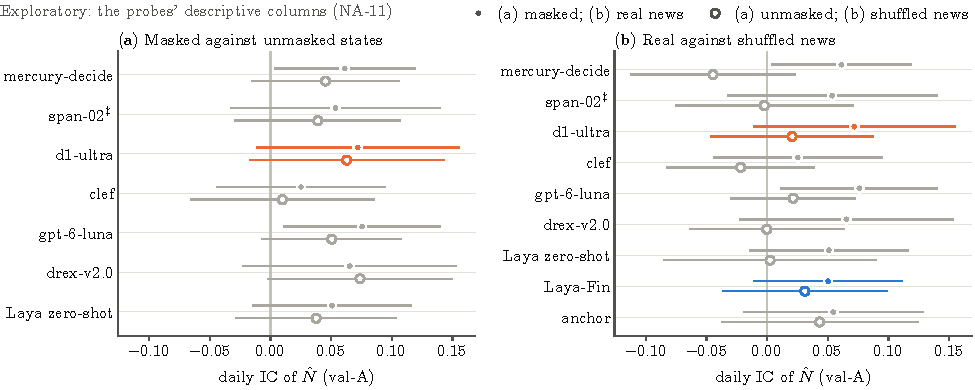
\includegraphics{figA13_probes.pdf}
\caption{\textbf{Exploratory: the probes' descriptive columns.} Exploratory (post hoc): the probes' descriptive columns (NA-11, val-A), not hypotheses. (a) ICs on masked and unmasked states: unmasking does not raise them materially (d1-ultra 0.072 masked and 0.063 unmasked; the largest rise, drex-v2.0's, is +0.01, t 0.48). Both panels share the IC scale. (b) ICs on real against shuffled news on the same events (Laya-Fin 0.050 and 0.031, inconclusive); the anchor is uninformative (near-constant outputs). $\ddagger$ span-02: the S5 canary fired a STOP after the freeze and the operator chose to proceed (PREREG \S{}15).}\label{fig:figA13_probes}
\end{figure}

\clearpage

% t21_release_dates (NA-14, from artifacts/NA-05/catalog.json, artifacts/NA-14/inputs/operator.yaml, artifacts/NA-12/results/monthly_ic.json, configs/splits.yaml)
\begin{table}[tbp]
\centering\small
\caption{Release dates of the decision models against the sample (test period ends at sample\_end)}\label{tab:t21_release_dates}
\begin{adjustbox}{max width=\linewidth}
\begin{tabular}{>{\raggedright\arraybackslash}p{12em}lr>{\raggedright\arraybackslash}p{12em}}
\toprule
name & date & days after sample end & source \\
\midrule
end of the test period (configs/splits.yaml) & 2026-07-31 & $0.000$ & configs/splits.yaml \\
Convai Laya (open weights; the base of Laya-Fin and of Laya zero-shot) & 2026-09-18 & $49.000$ & operator, NA-14 preamble item 3 \\
nace-ai/drex-v2.0 & 2026-10-12 & $73.000$ & artifacts/NA-05/catalog.json (created) \\
liquid/d1-ultra & 2026-10-15 & $76.000$ & artifacts/NA-05/catalog.json (created) \\
respan/span-02\textsuperscript{\ddag} & 2026-10-16 & $77.000$ & artifacts/NA-05/catalog.json (created) \\
answerdotai/ModernBERT-large checkpoint (the anchor) & 2024-12 & --- & answerdotai/ModernBERT-large Dec-2024 checkpoint (PREREG \S{}9.2) \\
\bottomrule
\end{tabular}
\end{adjustbox}
\par\smallskip{\footnotesize\raggedright Days after the end of the test period; the anchor's checkpoint is known to the month only. The anchor's readings are uninformative (near-constant outputs: NA-11 REPORT \S{}7.1 item 4); its rows are reported, not read as nulls. \textsuperscript{\ddag} span-02: the S5 canary fired a STOP after the freeze; the operator chose to proceed (PREREG \S{}15, the post-freeze NA-11 S5 row).\par}
\end{table}


\clearpage

% t23_company_identification: tab:a-company-identification (NA-14 figures.latex, from artifacts/NA-14/tables/t23_company_identification.csv)
\begin{table}[htbp]
\centering
\small
\begin{threeparttable}
\caption{Company identification on masked states: the API models name the company far above the matched baseline.}\label{tab:a-company-identification}
\begin{tabular}{@{}lS[table-format=1.3]S[table-format=3.0]S[table-format=1.3]S[table-format=1.2]@{}}
\toprule
Model & {Identified} & {States} & {Matched baseline} & {Screen bar} \\
\midrule
clef & 0.660 & 400 & 0.282 & 0.40 \\
mercury-decide & 0.620 & 400 & 0.282 & 0.40 \\
d1-ultra & 0.743 & 400 & 0.282 & 0.40 \\
Laya zero-shot & 0.320 & 400 & 0.282 & 0.40 \\
drex-v2.0 & 0.680 & 400 & 0.282 & 0.40 \\
gpt-6-luna & 0.682 & 399 & 0.282 & 0.40 \\
span-02$^{\ddagger}$ & 0.662 & 400 & 0.282 & 0.40 \\
\bottomrule
\end{tabular}
\begin{tablenotes}[flushleft]\footnotesize
\item NA-06's val-A events with activity-matched distractors (NA-11); States: the valid answers.
\item $^{\ddagger}$span-02: after the freeze, a stability check that repeats earlier requests (the canary) fired for it; its build was unchanged, and production went ahead under a rule recorded in the deviations log.
\end{tablenotes}
\end{threeparttable}
\end{table}


\clearpage

% t18_probes_val_a (NA-14, from artifacts/NA-12/tables/t18_probes_val_a.csv)
\begin{table*}[tbp]
\centering\small
\caption{Disclosed val-A probes (NA-11; not hypotheses), next to the model comparison}\label{tab:t18_probes_val_a}
\begin{adjustbox}{max width=\textwidth}
\begin{tabular}{lrrrrrrrrrrrrrrrrrrrrrrrrrl>{\raggedright\arraybackslash}p{12em}llll}
\toprule
model & flip rate & flip pairs & flip screen & edit mean shift & flip rate all pairs & flip pairs valid & right way & edit shift t & \^{N} sd val-A & shift sd & IC masked & IC masked t & IC unmasked & IC unmasked t & unmasked minus masked & unmasked minus masked t & masked screen & IC shuffled & IC shuffled t & shuffled screen t & IC real same events & IC real same events t & real minus shuffled & real minus shuffled t & real shuffled events & kind & screen company identification & screen counterfactual flip & screen masked vs unmasked & screen shuffled news & screen all \\
\midrule
inception/mercury-decide & $0.562$ & $169$ & $0.700$ & $1.144$ & $0.550$ & $200$ & $0.995$ & $18.964$ & $0.819$ & $1.397$ & $0.061$ & $2.069$ & $0.045$ & $1.459$ & $-0.016$ & $-1.012$ & $0.020$ & $-0.044$ & $-1.284$ & $2$ & $0.061$ & $2.069$ & $0.106$ & $2.805$ & $1{,}000$ & api (NA-06 stage 2) & no & no & yes & yes & no \\
respan/span-02\textsuperscript{\ddag} & $0.645$ & $169$ & $0.700$ & $1.364$ & $0.650$ & $200$ & $0.990$ & $20.801$ & $0.847$ & $1.610$ & $0.054$ & $1.214$ & $0.039$ & $1.121$ & $-0.015$ & $-0.800$ & $0.020$ & $-0.002$ & $-0.062$ & $2$ & $0.054$ & $1.214$ & $0.056$ & $0.984$ & $1{,}000$ & api (NA-06 stage 2) & no & no & yes & yes & no \\
liquid/d1-ultra & $0.678$ & $177$ & $0.700$ & $1.093$ & $0.680$ & $200$ & $0.985$ & $21.552$ & $0.599$ & $1.826$ & $0.072$ & $1.689$ & $0.063$ & $1.532$ & $-0.009$ & $-0.426$ & $0.020$ & $0.021$ & $0.604$ & $2$ & $0.072$ & $1.689$ & $0.051$ & $1.033$ & $1{,}000$ & api (NA-06 stage 2) & no & no & yes & yes & no \\
cloudflare/clef & $0.529$ & $155$ & $0.700$ & $0.803$ & $0.500$ & $200$ & $0.980$ & $19.729$ & $0.650$ & $1.236$ & $0.025$ & $0.711$ & $0.010$ & $0.257$ & $-0.015$ & $-1.071$ & $0.020$ & $-0.022$ & $-0.697$ & $2$ & $0.025$ & $0.711$ & $0.047$ & $1.092$ & $1{,}000$ & api (NA-06 stage 2) & no & no & yes & yes & no \\
openai/gpt-6-luna-decisions & $0.568$ & $148$ & $0.700$ & $0.918$ & $0.610$ & $200$ & $0.950$ & $17.569$ & $0.625$ & $1.468$ & $0.076$ & $2.291$ & $0.051$ & $1.721$ & $-0.025$ & $-0.980$ & $0.020$ & $0.021$ & $0.819$ & $2$ & $0.076$ & $2.305$ & $0.056$ & $1.457$ & $997$ & api (NA-06 stage 2) & no & no & yes & yes & no \\
nace-ai/drex-v2.0 & $0.710$ & $162$ & $0.700$ & $1.022$ & $0.650$ & $200$ & $0.985$ & $22.186$ & $0.641$ & $1.593$ & $0.065$ & $1.451$ & $0.074$ & $1.891$ & $0.008$ & $0.477$ & $0.020$ & $-2.79\times 10^{-4}$ & $-0.009$ & $2$ & $0.065$ & $1.451$ & $0.066$ & $1.162$ & $1{,}000$ & api (NA-06 stage 2) & no & yes & yes & yes & no \\
local/laya-typed-decisions & $0.043$ & $92$ & $0.700$ & $0.134$ & $0.125$ & $200$ & $0.940$ & $11.226$ & $0.325$ & $0.413$ & $0.051$ & $1.522$ & $0.038$ & $1.112$ & $-0.013$ & $-0.506$ & $0.020$ & $0.002$ & $0.054$ & $2$ & $0.051$ & $1.522$ & $0.048$ & $1.285$ & $1{,}000$ & local zero-shot & --- & --- & --- & --- & --- \\
Laya-Fin & $0.000$ & $8$ & $0.700$ & $0.021$ & $0.125$ & $200$ & $0.800$ & $7.349$ & $0.105$ & $0.202$ & --- & --- & --- & --- & --- & --- & --- & $0.031$ & $0.896$ & $2$ & $0.050$ & $1.597$ & $0.019$ & $0.465$ & $1{,}000$ & trained (S7) & --- & --- & --- & --- & --- \\
anchor (uninformative) & --- & $0$ & $0.700$ & $1.17\times 10^{-6}$ & $0.000$ & $200$ & $0.435$ & $0.185$ & $0.006$ & $1.90\times 10^{-4}$ & --- & --- & --- & --- & --- & --- & --- & $0.043$ & $1.045$ & $2$ & $0.055$ & $1.444$ & $0.011$ & $0.939$ & $1{,}000$ & trained (S7) & --- & --- & --- & --- & --- \\
\bottomrule
\end{tabular}
\end{adjustbox}
\par\smallskip{\footnotesize\raggedright The anchor's readings are uninformative (near-constant outputs: NA-11 REPORT \S{}7.1 item 4); its rows are reported, not read as nulls. \textsuperscript{\ddag} span-02: the S5 canary fired a STOP after the freeze; the operator chose to proceed (PREREG \S{}15, the post-freeze NA-11 S5 row).\par}
\end{table*}


\clearpage

\section{Exploratory analyses (post hoc)}

\begin{figure}[htbp]
\centering
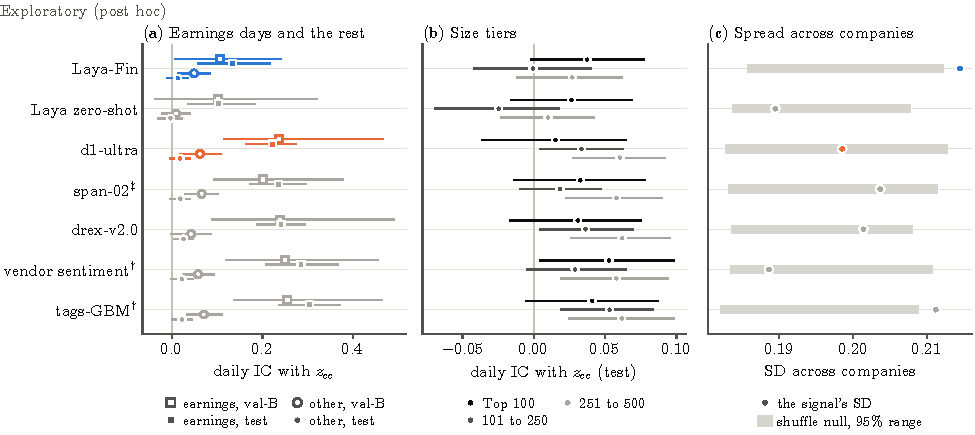
\includegraphics{figA14_exploratory_d0.pdf}
\caption{\textbf{Exploratory (post hoc): where the D0 signal lives.} Exploratory (post hoc): requested after unblinding (NA-12 \S{}13); no hypothesis, no claim. (a) Every signal's IC sits on earnings-day events (squares), and there it held from val-B (hollow) to test (filled): Laya-Fin 0.11 and 0.13, d1-ultra 0.24 and 0.22. On other events (circles) it fell, for Laya-Fin from 0.049 to 0.013, and for every other signal too. (b) By size tier on test the API models' IC sits in the two smaller tiers (d1-ultra 0.015 in the Top-100 against 0.060 in the 251--500 tier). The earnings-day ICs of (a) are several times the tier ICs of (b), so the two panels have their own scales. (c) The spread of the per-company rank correlations against a within-company shuffle (gray: its 95\% range): Laya-Fin's (0.214, p 0.015) and tags-GBM's exceed it, the others' do not; the test cannot tell company-specific skill from company-specific noise. Not drawn: a one-way test of the daily ICs on the calendar month finds no month effect on test (p 0.72 for Laya-Fin and 0.44 for d1-ultra). $\dagger$ Vendor-label baselines: a possibly look-ahead-contaminated upper bound. $\ddagger$ span-02: the S5 canary fired a STOP after the freeze and the operator chose to proceed (PREREG \S{}15).}\label{fig:figA14_exploratory_d0}
\end{figure}

\clearpage

\begin{figure}[htbp]
\centering
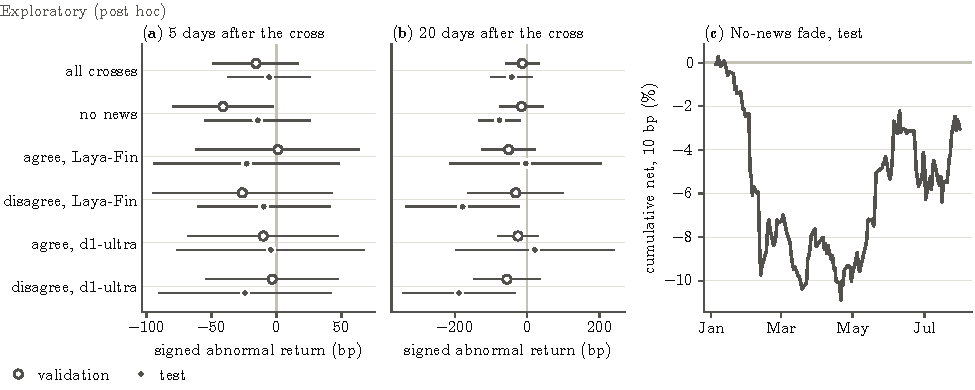
\includegraphics{figA15_exploratory_ma_cross.pdf}
\caption{\textbf{Exploratory (post hoc): news and a moving-average cross.} Exploratory (post hoc): the operator's MA20/MA50 cross add-on (NA-13 \S{}9), designed on validation and run once on test; no claim. (a, b) Mean signed abnormal return over 5 and 20 days after a cross, by group (95\% intervals, $\pm$1.96 Newey--West SE), validation (hollow) against test (filled); the two panels have their own scales, since 20-day returns spread wider than 5-day ones. The validation reversal of crosses without news ($-$41.1 bp, t $-$2.08) did not replicate on test ($-$14.4 bp, t $-$0.69). (c) The tradable no-news fade on test, cumulative net at 10 bp: net Sharpe $-$0.46 (gross 0.98, after 3.85 on validation, where its design was chosen).}\label{fig:figA15_exploratory_ma_cross}
\end{figure}

\clearpage

% t17_sector_exploratory (NA-14, from artifacts/NA-12/tables/t17_sector_exploratory.csv)
\begin{landscape}
{\scriptsize\setlength{\tabcolsep}{3pt}
\begin{longtable}{lllrrrrrrr}
\caption{Exploratory (outside every family, no claim): IC of \^{N}\_W0 by GICS sector and leave-one-sector-out}\label{tab:t17_sector_exploratory}\\
\toprule
model & kind & sector & IC z-cc & IC z-cc t & IC z-cc n & IC z-on & IC z-on t & IC z-id & IC z-id t \\
\midrule
\endfirsthead
\toprule
model & kind & sector & IC z-cc & IC z-cc t & IC z-cc n & IC z-on & IC z-on t & IC z-id & IC z-id t \\
\midrule
\endhead
\bottomrule
\endfoot
Laya-Fin & by\_sector & Communication Services & $0.049$ & $0.702$ & $524$ & $-0.031$ & $-0.466$ & $0.035$ & $0.557$ \\
Laya-Fin & by\_sector & Consumer Discretionary & $0.063$ & $2.216$ & $1{,}381$ & $0.032$ & $0.955$ & $0.023$ & $0.643$ \\
Laya-Fin & by\_sector & Consumer Staples & $0.052$ & $1.181$ & $934$ & $0.070$ & $1.557$ & $-0.026$ & $-0.904$ \\
Laya-Fin & by\_sector & Energy & $-0.046$ & $-0.851$ & $531$ & $-0.009$ & $-0.141$ & $-0.082$ & $-1.680$ \\
Laya-Fin & by\_sector & Financials & $0.045$ & $1.468$ & $1{,}798$ & $0.012$ & $0.389$ & $0.036$ & $1.358$ \\
Laya-Fin & by\_sector & Health Care & $0.043$ & $1.510$ & $1{,}999$ & $0.034$ & $1.189$ & $0.030$ & $1.045$ \\
Laya-Fin & by\_sector & Industrials & $-0.030$ & $-1.247$ & $2{,}408$ & $-0.003$ & $-0.122$ & $-0.025$ & $-1.085$ \\
Laya-Fin & by\_sector & Information Technology & $0.036$ & $1.408$ & $2{,}587$ & $-0.021$ & $-0.778$ & $0.035$ & $1.220$ \\
Laya-Fin & by\_sector & Materials & $-0.043$ & $-0.813$ & $435$ & $-0.068$ & $-1.435$ & $-0.097$ & $-1.624$ \\
Laya-Fin & by\_sector & Real Estate & $0.100$ & $1.198$ & $431$ & $0.043$ & $0.433$ & $0.124$ & $2.026$ \\
Laya-Fin & by\_sector & Utilities & $-0.035$ & $-0.560$ & $720$ & $0.074$ & $1.411$ & $-0.113$ & $-1.512$ \\
Laya-Fin & leave\_one\_out & Communication Services & $0.020$ & $1.610$ & $13{,}224$ & $0.013$ & $0.898$ & $0.012$ & $0.909$ \\
Laya-Fin & leave\_one\_out & Consumer Discretionary & $0.022$ & $1.762$ & $12{,}367$ & $0.012$ & $0.841$ & $0.012$ & $0.900$ \\
Laya-Fin & leave\_one\_out & Consumer Staples & $0.017$ & $1.323$ & $12{,}814$ & $0.017$ & $1.222$ & $0.007$ & $0.511$ \\
Laya-Fin & leave\_one\_out & Energy & $0.021$ & $1.722$ & $13{,}217$ & $0.014$ & $1.004$ & $0.012$ & $0.950$ \\
Laya-Fin & leave\_one\_out & Financials & $0.016$ & $1.129$ & $11{,}950$ & $0.010$ & $0.621$ & $0.007$ & $0.480$ \\
Laya-Fin & leave\_one\_out & Health Care & $0.016$ & $1.321$ & $11{,}749$ & $0.009$ & $0.668$ & $0.006$ & $0.501$ \\
Laya-Fin & leave\_one\_out & Industrials & $0.030$ & $2.322$ & $11{,}340$ & $0.016$ & $1.011$ & $0.020$ & $1.523$ \\
Laya-Fin & leave\_one\_out & Information Technology & $0.011$ & $1.003$ & $11{,}161$ & $0.026$ & $1.901$ & $5.55\times 10^{-4}$ & $0.046$ \\
Laya-Fin & leave\_one\_out & Materials & $0.021$ & $1.789$ & $13{,}313$ & $0.016$ & $1.094$ & $0.012$ & $0.943$ \\
Laya-Fin & leave\_one\_out & Real Estate & $0.020$ & $1.626$ & $13{,}317$ & $0.016$ & $1.136$ & $0.010$ & $0.767$ \\
Laya-Fin & leave\_one\_out & Utilities & $0.024$ & $1.989$ & $13{,}028$ & $0.018$ & $1.236$ & $0.014$ & $1.072$ \\
anchor (uninformative) & by\_sector & Communication Services & $0.033$ & $0.610$ & $524$ & $-0.102$ & $-2.143$ & $0.058$ & $1.424$ \\
anchor (uninformative) & by\_sector & Consumer Discretionary & $0.008$ & $0.217$ & $1{,}381$ & $0.060$ & $1.985$ & $-0.037$ & $-1.071$ \\
anchor (uninformative) & by\_sector & Consumer Staples & $-0.095$ & $-2.059$ & $934$ & $-0.028$ & $-0.605$ & $-0.098$ & $-2.492$ \\
anchor (uninformative) & by\_sector & Energy & $-0.003$ & $-0.065$ & $531$ & $-0.003$ & $-0.043$ & $-0.008$ & $-0.160$ \\
anchor (uninformative) & by\_sector & Financials & $0.060$ & $2.295$ & $1{,}798$ & $-0.005$ & $-0.213$ & $0.081$ & $3.120$ \\
anchor (uninformative) & by\_sector & Health Care & $0.017$ & $0.497$ & $1{,}999$ & $0.018$ & $0.606$ & $-0.003$ & $-0.075$ \\
anchor (uninformative) & by\_sector & Industrials & $-0.018$ & $-0.580$ & $2{,}408$ & $-0.048$ & $-2.192$ & $-0.003$ & $-0.084$ \\
anchor (uninformative) & by\_sector & Information Technology & $0.049$ & $2.484$ & $2{,}587$ & $0.021$ & $0.831$ & $0.030$ & $1.373$ \\
anchor (uninformative) & by\_sector & Materials & $-0.061$ & $-1.172$ & $435$ & $-0.102$ & $-1.340$ & $-0.089$ & $-1.784$ \\
anchor (uninformative) & by\_sector & Real Estate & $0.004$ & $0.074$ & $431$ & $-0.070$ & $-1.375$ & $0.067$ & $0.764$ \\
anchor (uninformative) & by\_sector & Utilities & $-0.037$ & $-0.816$ & $720$ & $-0.128$ & $-2.600$ & $0.033$ & $1.215$ \\
anchor (uninformative) & leave\_one\_out & Communication Services & $0.009$ & $0.986$ & $13{,}224$ & $0.002$ & $0.206$ & $0.006$ & $0.502$ \\
anchor (uninformative) & leave\_one\_out & Consumer Discretionary & $0.009$ & $0.831$ & $12{,}367$ & $-0.002$ & $-0.194$ & $0.007$ & $0.607$ \\
anchor (uninformative) & leave\_one\_out & Consumer Staples & $0.011$ & $1.134$ & $12{,}814$ & $0.008$ & $0.650$ & $0.006$ & $0.509$ \\
anchor (uninformative) & leave\_one\_out & Energy & $0.012$ & $1.276$ & $13{,}217$ & $0.006$ & $0.506$ & $0.006$ & $0.553$ \\
anchor (uninformative) & leave\_one\_out & Financials & $0.004$ & $0.426$ & $11{,}950$ & $0.006$ & $0.480$ & $-0.003$ & $-0.310$ \\
anchor (uninformative) & leave\_one\_out & Health Care & $0.006$ & $0.601$ & $11{,}749$ & $0.002$ & $0.193$ & $0.003$ & $0.213$ \\
anchor (uninformative) & leave\_one\_out & Industrials & $0.007$ & $0.682$ & $11{,}340$ & $0.018$ & $1.665$ & $-0.006$ & $-0.496$ \\
anchor (uninformative) & leave\_one\_out & Information Technology & $-0.001$ & $-0.107$ & $11{,}161$ & $-5.14\times 10^{-4}$ & $-0.039$ & $-0.004$ & $-0.333$ \\
anchor (uninformative) & leave\_one\_out & Materials & $0.008$ & $0.892$ & $13{,}313$ & $0.008$ & $0.725$ & $0.002$ & $0.200$ \\
anchor (uninformative) & leave\_one\_out & Real Estate & $0.008$ & $0.821$ & $13{,}317$ & $0.005$ & $0.418$ & $0.003$ & $0.249$ \\
anchor (uninformative) & leave\_one\_out & Utilities & $0.008$ & $0.785$ & $13{,}028$ & $0.009$ & $0.854$ & $-4.39\times 10^{-4}$ & $-0.038$ \\
d1-ultra & by\_sector & Communication Services & $0.103$ & $1.786$ & $524$ & $0.091$ & $1.395$ & $0.010$ & $0.151$ \\
d1-ultra & by\_sector & Consumer Discretionary & $0.087$ & $2.640$ & $1{,}381$ & $0.080$ & $1.807$ & $0.008$ & $0.254$ \\
d1-ultra & by\_sector & Consumer Staples & $0.069$ & $1.898$ & $934$ & $0.057$ & $1.509$ & $0.020$ & $0.505$ \\
d1-ultra & by\_sector & Energy & $0.120$ & $1.925$ & $531$ & $0.095$ & $1.052$ & $0.047$ & $0.933$ \\
d1-ultra & by\_sector & Financials & $0.044$ & $1.611$ & $1{,}798$ & $0.092$ & $2.724$ & $-0.002$ & $-0.067$ \\
d1-ultra & by\_sector & Health Care & $0.055$ & $1.736$ & $1{,}999$ & $0.082$ & $2.638$ & $0.050$ & $1.527$ \\
d1-ultra & by\_sector & Industrials & $0.007$ & $0.282$ & $2{,}408$ & $0.049$ & $1.632$ & $-0.026$ & $-0.957$ \\
d1-ultra & by\_sector & Information Technology & $0.034$ & $1.249$ & $2{,}587$ & $0.063$ & $2.219$ & $0.003$ & $0.133$ \\
d1-ultra & by\_sector & Materials & $0.008$ & $0.156$ & $435$ & $0.064$ & $0.688$ & $-0.022$ & $-0.379$ \\
d1-ultra & by\_sector & Real Estate & $0.090$ & $1.077$ & $431$ & $0.055$ & $0.516$ & $-0.009$ & $-0.062$ \\
d1-ultra & by\_sector & Utilities & $-0.084$ & $-1.932$ & $720$ & $0.038$ & $0.649$ & $-0.124$ & $-2.913$ \\
d1-ultra & leave\_one\_out & Communication Services & $0.040$ & $3.261$ & $13{,}224$ & $0.074$ & $4.621$ & $-8.46\times 10^{-4}$ & $-0.074$ \\
d1-ultra & leave\_one\_out & Consumer Discretionary & $0.035$ & $2.714$ & $12{,}367$ & $0.067$ & $4.252$ & $-0.002$ & $-0.197$ \\
d1-ultra & leave\_one\_out & Consumer Staples & $0.039$ & $3.159$ & $12{,}814$ & $0.076$ & $4.613$ & $0.001$ & $0.099$ \\
d1-ultra & leave\_one\_out & Energy & $0.040$ & $3.200$ & $13{,}217$ & $0.075$ & $4.558$ & $-7.35\times 10^{-4}$ & $-0.066$ \\
d1-ultra & leave\_one\_out & Financials & $0.041$ & $3.454$ & $11{,}950$ & $0.071$ & $4.544$ & $0.004$ & $0.339$ \\
d1-ultra & leave\_one\_out & Health Care & $0.030$ & $2.200$ & $11{,}749$ & $0.067$ & $3.981$ & $-0.010$ & $-0.912$ \\
d1-ultra & leave\_one\_out & Industrials & $0.040$ & $2.854$ & $11{,}340$ & $0.075$ & $4.583$ & $0.002$ & $0.168$ \\
d1-ultra & leave\_one\_out & Information Technology & $0.043$ & $3.722$ & $11{,}161$ & $0.081$ & $5.346$ & $-0.002$ & $-0.198$ \\
d1-ultra & leave\_one\_out & Materials & $0.040$ & $3.220$ & $13{,}313$ & $0.075$ & $4.573$ & $1.84\times 10^{-4}$ & $0.017$ \\
d1-ultra & leave\_one\_out & Real Estate & $0.039$ & $3.170$ & $13{,}317$ & $0.075$ & $4.818$ & $-0.001$ & $-0.102$ \\
d1-ultra & leave\_one\_out & Utilities & $0.043$ & $3.536$ & $13{,}028$ & $0.078$ & $4.953$ & $0.002$ & $0.164$ \\
\end{longtable}
\par\smallskip{\footnotesize\raggedright Exploratory (post hoc): requested after unblinding; no hypothesis, outside every family, no claim. Selected columns; every cell is in t17\_sector\_exploratory.csv. The anchor's readings are uninformative (near-constant outputs: NA-11 REPORT \S{}7.1 item 4); its rows are reported, not read as nulls.\par}
}
\end{landscape}


\clearpage

% t25_ma_cross (NA-14, from artifacts/NA-13/results/ma_cross.json)
\begin{table*}[tbp]
\centering\small
\caption{News and an MA20/MA50 cross (NA-13 \S{}9, operator item 9): group statistics and the no-news fade}\label{tab:t25_ma_cross}
\begin{adjustbox}{max width=\textwidth}
\begin{tabular}{>{\raggedright\arraybackslash}p{12em}lrrrrrrrrr}
\toprule
key & group & horizon & mean bp & NW t & n days & n crosses & sharpe gross & sharpe net 10 & placebo pct gross & capacity median USD \\
\midrule
periods:\allowbreak{}validation:\allowbreak{}statistics:\allowbreak{}all$|$\allowbreak{}5 & all & $5.000$ & $-15.841$ & $-0.936$ & $123$ & $1{,}293$ & --- & --- & --- & --- \\
periods:\allowbreak{}validation:\allowbreak{}statistics:\allowbreak{}all$|$\allowbreak{}20 & all & $20.000$ & $-13.921$ & $-0.582$ & $108$ & $1{,}132$ & --- & --- & --- & --- \\
periods:\allowbreak{}validation:\allowbreak{}statistics:\allowbreak{}none$|$\allowbreak{}5 & none & $5.000$ & $-41.133$ & $-2.078$ & $122$ & $686$ & --- & --- & --- & --- \\
periods:\allowbreak{}validation:\allowbreak{}statistics:\allowbreak{}none$|$\allowbreak{}20 & none & $20.000$ & $-15.785$ & $-0.515$ & $107$ & $568$ & --- & --- & --- & --- \\
periods:\allowbreak{}validation:\allowbreak{}statistics:\allowbreak{}agree\_\allowbreak{}laya\_\allowbreak{}fin$|$\allowbreak{}5 & agree\_laya\_fin & $5.000$ & $1.129$ & $0.035$ & $110$ & $351$ & --- & --- & --- & --- \\
periods:\allowbreak{}validation:\allowbreak{}statistics:\allowbreak{}agree\_\allowbreak{}laya\_\allowbreak{}fin$|$\allowbreak{}20 & agree\_laya\_fin & $20.000$ & $-51.314$ & $-1.338$ & $97$ & $328$ & --- & --- & --- & --- \\
periods:\allowbreak{}validation:\allowbreak{}statistics:\allowbreak{}disagree\_\allowbreak{}laya\_\allowbreak{}fin$|$\allowbreak{}5 & disagree\_laya\_fin & $5.000$ & $-26.282$ & $-0.745$ & $107$ & $256$ & --- & --- & --- & --- \\
periods:\allowbreak{}validation:\allowbreak{}statistics:\allowbreak{}disagree\_\allowbreak{}laya\_\allowbreak{}fin$|$\allowbreak{}20 & disagree\_laya\_fin & $20.000$ & $-31.873$ & $-0.470$ & $96$ & $236$ & --- & --- & --- & --- \\
periods:\allowbreak{}validation:\allowbreak{}statistics:\allowbreak{}agree\_\allowbreak{}d1\_\allowbreak{}ultra$|$\allowbreak{}5 & agree\_d1\_ultra & $5.000$ & $-10.263$ & $-0.347$ & $106$ & $327$ & --- & --- & --- & --- \\
periods:\allowbreak{}validation:\allowbreak{}statistics:\allowbreak{}agree\_\allowbreak{}d1\_\allowbreak{}ultra$|$\allowbreak{}20 & agree\_d1\_ultra & $20.000$ & $-25.586$ & $-0.869$ & $93$ & $304$ & --- & --- & --- & --- \\
periods:\allowbreak{}validation:\allowbreak{}statistics:\allowbreak{}disagree\_\allowbreak{}d1\_\allowbreak{}ultra$|$\allowbreak{}5 & disagree\_d1\_ultra & $5.000$ & $-3.293$ & $-0.126$ & $103$ & $280$ & --- & --- & --- & --- \\
periods:\allowbreak{}validation:\allowbreak{}statistics:\allowbreak{}disagree\_\allowbreak{}d1\_\allowbreak{}ultra$|$\allowbreak{}20 & disagree\_d1\_ultra & $20.000$ & $-56.084$ & $-1.173$ & $93$ & $260$ & --- & --- & --- & --- \\
periods:\allowbreak{}validation:\allowbreak{}fade\_\allowbreak{}no\_\allowbreak{}news & --- & --- & --- & --- & $127$ & --- & $3.850$ & $1.830$ & $99.000$ & $33616464.622$ \\
periods:\allowbreak{}test:\allowbreak{}statistics:\allowbreak{}all$|$\allowbreak{}5 & all & $5.000$ & $-5.618$ & $-0.343$ & $140$ & $1{,}580$ & --- & --- & --- & --- \\
periods:\allowbreak{}test:\allowbreak{}statistics:\allowbreak{}all$|$\allowbreak{}20 & all & $20.000$ & $-42.891$ & $-1.446$ & $125$ & $1{,}444$ & --- & --- & --- & --- \\
periods:\allowbreak{}test:\allowbreak{}statistics:\allowbreak{}none$|$\allowbreak{}5 & none & $5.000$ & $-14.414$ & $-0.691$ & $138$ & $919$ & --- & --- & --- & --- \\
periods:\allowbreak{}test:\allowbreak{}statistics:\allowbreak{}none$|$\allowbreak{}20 & none & $20.000$ & $-76.691$ & $-2.552$ & $123$ & $847$ & --- & --- & --- & --- \\
periods:\allowbreak{}test:\allowbreak{}statistics:\allowbreak{}agree\_\allowbreak{}laya\_\allowbreak{}fin$|$\allowbreak{}5 & agree\_laya\_fin & $5.000$ & $-23.073$ & $-0.634$ & $123$ & $371$ & --- & --- & --- & --- \\
periods:\allowbreak{}test:\allowbreak{}statistics:\allowbreak{}agree\_\allowbreak{}laya\_\allowbreak{}fin$|$\allowbreak{}20 & agree\_laya\_fin & $20.000$ & $-4.326$ & $-0.040$ & $110$ & $340$ & --- & --- & --- & --- \\
periods:\allowbreak{}test:\allowbreak{}statistics:\allowbreak{}disagree\_\allowbreak{}laya\_\allowbreak{}fin$|$\allowbreak{}5 & disagree\_laya\_fin & $5.000$ & $-9.841$ & $-0.376$ & $117$ & $290$ & --- & --- & --- & --- \\
periods:\allowbreak{}test:\allowbreak{}statistics:\allowbreak{}disagree\_\allowbreak{}laya\_\allowbreak{}fin$|$\allowbreak{}20 & disagree\_laya\_fin & $20.000$ & $-178.802$ & $-2.225$ & $103$ & $257$ & --- & --- & --- & --- \\
periods:\allowbreak{}test:\allowbreak{}statistics:\allowbreak{}agree\_\allowbreak{}d1\_\allowbreak{}ultra$|$\allowbreak{}5 & agree\_d1\_ultra & $5.000$ & $-4.362$ & $-0.118$ & $119$ & $371$ & --- & --- & --- & --- \\
periods:\allowbreak{}test:\allowbreak{}statistics:\allowbreak{}agree\_\allowbreak{}d1\_\allowbreak{}ultra$|$\allowbreak{}20 & agree\_d1\_ultra & $20.000$ & $20.945$ & $0.187$ & $107$ & $343$ & --- & --- & --- & --- \\
periods:\allowbreak{}test:\allowbreak{}statistics:\allowbreak{}disagree\_\allowbreak{}d1\_\allowbreak{}ultra$|$\allowbreak{}5 & disagree\_d1\_ultra & $5.000$ & $-24.275$ & $-0.712$ & $121$ & $290$ & --- & --- & --- & --- \\
periods:\allowbreak{}test:\allowbreak{}statistics:\allowbreak{}disagree\_\allowbreak{}d1\_\allowbreak{}ultra$|$\allowbreak{}20 & disagree\_d1\_ultra & $20.000$ & $-188.737$ & $-2.348$ & $106$ & $254$ & --- & --- & --- & --- \\
periods:\allowbreak{}test:\allowbreak{}fade\_\allowbreak{}no\_\allowbreak{}news & --- & --- & --- & --- & $144$ & --- & $0.977$ & $-0.463$ & $81.000$ & $47183426.249$ \\
\bottomrule
\end{tabular}
\end{adjustbox}
\par\smallskip{\footnotesize\raggedright Exploratory (post hoc): requested after unblinding; no hypothesis, outside every family, no claim. Copied from artifacts/NA-13/results/ma\_cross.json; key = JSON path. Selected columns and rows; every cell is in t25\_ma\_cross.csv.\par}
\end{table*}


\clearpage

% t31_market_replication: tab:a-market-replication (NA-14 figures.latex, from artifacts/NA-14/tables/t31_market_replication.csv)
\begin{table}[htbp]
\centering
\small
\begin{threeparttable}
\caption{Exploratory: the A3.5 market-level replication.}\label{tab:a-market-replication}
\begin{tabular}{@{}lS[table-format=1.3]S[table-format=1.3]S[table-format=3.0]@{}}
\toprule
Item & {OOS $R^2$} & {$p$} & {Sessions} \\
\midrule
SPY's daily return on d1-ultra's market reading & 0.021 & 0.309 & 144 \\
\bottomrule
\end{tabular}
\begin{tablenotes}[flushleft]\footnotesize
\item Exploratory (PREREG A3.5: optional, exploratory); fit on the validation sessions, evaluated on test.
\end{tablenotes}
\end{threeparttable}
\end{table}


\clearpage

\section{When the D0 signal works (exploratory, post hoc; NA-13b)}

\begin{figure}[htbp]
\centering
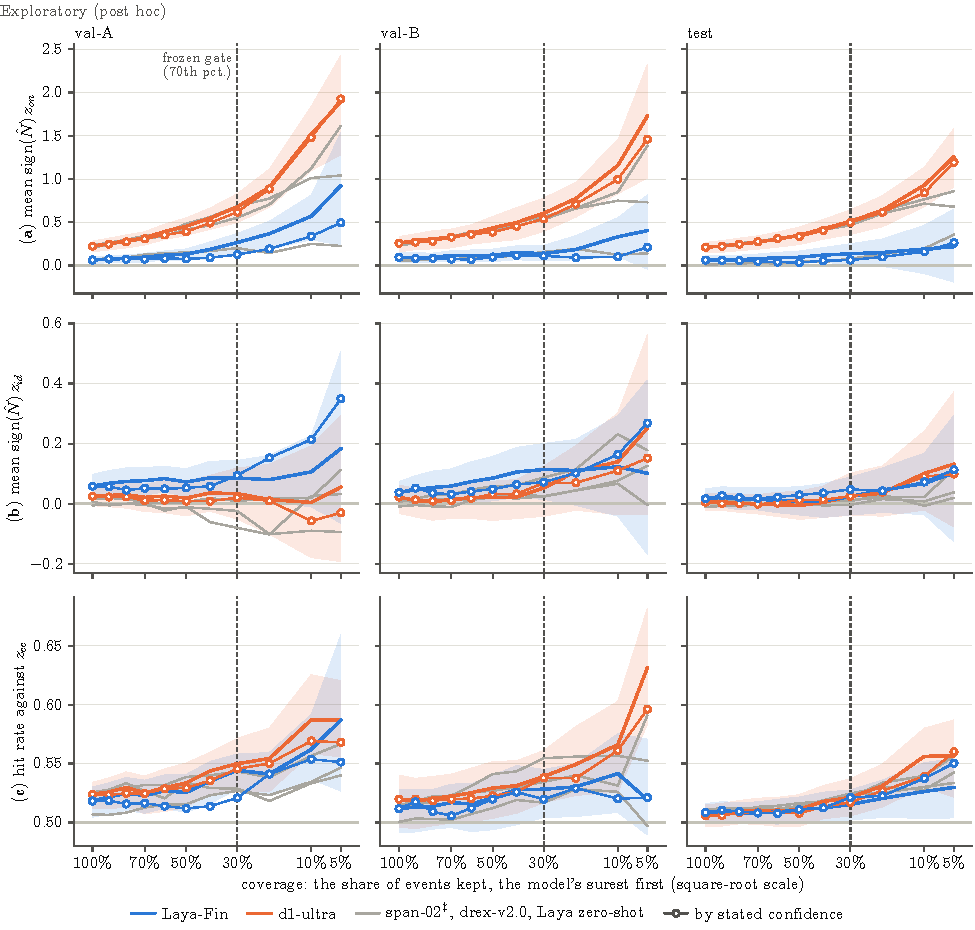
\includegraphics{figA16_selective_coverage.pdf}
\caption{\textbf{Exploratory (post hoc): risk-coverage curves of the pre-open reading.} Exploratory (post hoc): NA-13b, requested after unblinding; no hypothesis, no claim. Its thresholds come from val-A. The operator's assistant's first look by band of conviction, which used the test, came before this figure and shaped it (the band-check table in the appendix); no threshold is chosen from the curves. Each model's D0 events are ranked by its conviction $|\hat N|$ (solid lines) or, for Laya-Fin and d1-ultra, by its stated confidence (thin lines, hollow dots); a coverage keeps the events at or above the val-A quantile of the ranking. Rows: (a) the mean signed overnight move $\mathrm{sign}(\hat N)\,z_{on}$, (b) the mean signed move after the open $\mathrm{sign}(\hat N)\,z_{id}$, (c) the hit rate against $z_{cc}$; columns val-A, val-B and test; bands are 95\% bootstrap intervals; the dashed line is the frozen confidence gates' coverage (their val-A 70th percentile). Conviction concentrates the overnight move, which the open prices: d1-ultra's surest 10\% carry 0.93 typical moves on the test against 0.21 for all its events. After the open little is left: 0.10 (95\% interval $-$0.02 to 0.24) for d1-ultra's surest 10\% and 0.07 for Laya-Fin's; neither model's test interval excludes zero at any coverage. span-02's and drex-v2.0's val-A points come from NA-06's 3,000-event stage-2 sample. d1-ultra is model-specific (\S{}1.3). $\ddagger$ span-02: the S5 canary fired a STOP after the freeze and the operator chose to proceed (PREREG \S{}15).}\label{fig:figA16_selective_coverage}
\end{figure}

\clearpage

\begin{figure}[htbp]
\centering
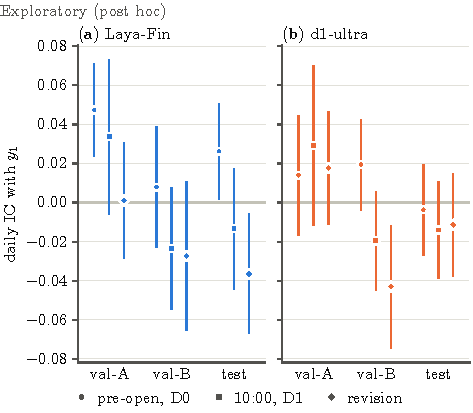
\includegraphics{figA17_watch_open.pdf}
\caption{\textbf{Exploratory (post hoc): the 10:00 reading against the pre-open one.} Exploratory (post hoc): NA-13b, requested after unblinding; no hypothesis, no claim. The operator's assistant computed the four ICs on all three splits before NA-13b; they are reproduced exactly. The daily IC with $y_1$, the move from 10:00 to the close, of the pre-open reading $\hat N_{\mathrm{D0}}$ (circles), of the 10:00 reading $\hat N_{\mathrm{D1}}$ (Call B at D1; squares) and of their revision $z(\hat N_{\mathrm{D1}}) - z(\hat N_{\mathrm{D0}})$ (diamonds) for (a) Laya-Fin and (b) d1-ultra on val-A, val-B and the test, with 95\% intervals ($\pm$1.96 Newey--West SE). Watching the open adds nothing: on val-B and the test the 10:00 reading's IC is negative for both models (test: Laya-Fin $-$0.013, d1-ultra $-$0.014), and so is the revision's (Laya-Fin on test $-$0.036, t $-$2.33); only Laya-Fin's pre-open reading keeps a positive test IC (0.026, t 2.09). The first bar, the moves after it and the pre-registered D1 results are in the appendix table on watching the open. With 36 statistics in that table, about two with $|t| > 2$ are expected by chance. d1-ultra is model-specific (\S{}1.3).}\label{fig:figA17_watch_open}
\end{figure}

\clearpage

\begin{figure}[htbp]
\centering
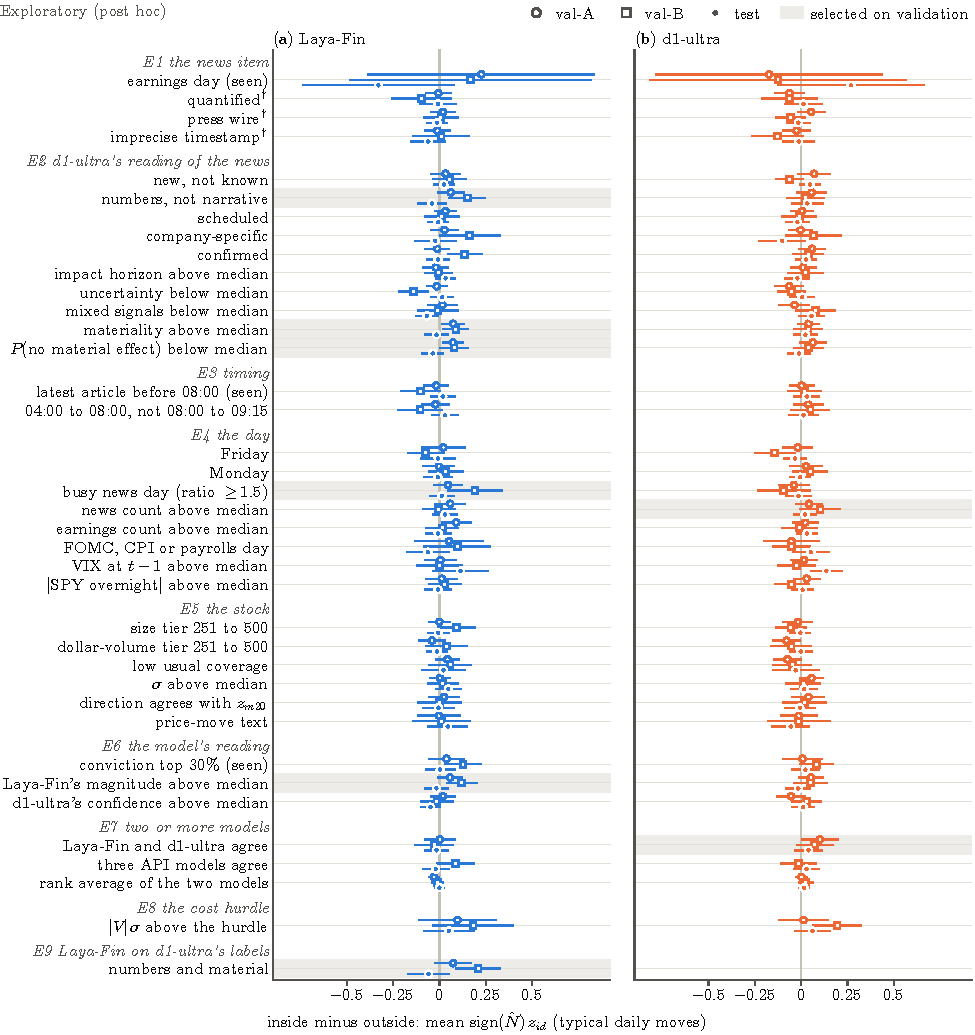
\includegraphics{figA18_conditioning_map.pdf}
\caption{\textbf{Exploratory (post hoc): the conditioning study, validation against test.} Exploratory (post hoc): NA-13b, requested after unblinding; no hypothesis, no claim. Thresholds and medians come from val-A; the selection used val-A and val-B only, by the operator's rule fixed before the test; the test was evaluated once. Each row: the difference inside minus outside of the primary outcome $\mathrm{sign}(\hat N)\,z_{id}$ (the move after the open) for (a) Laya-Fin and (b) d1-ultra on val-A (hollow circles), val-B (hollow squares) and the test (filled), with 95\% intervals ($\pm$1.96 $|$difference$/t|$). Shaded rows were selected on validation ($t \geq 1$ in val-A and in val-B, pooled $t \geq 2$). None held on the test: their test differences run from $-$0.06 (Laya-Fin's E9, the strongest on validation, pooled t 3.51) to +0.04 (d1-ultra's E7 agreement, t 1.01), every Benjamini--Hochberg q of the family is at least 0.79, and no pair is confirmed. (seen): seen on the test before the study, never selected. $\dagger$ Vendor labels produced retrospectively, possibly look-ahead-contaminated. E7's three-model agreement has no val-A run; its rank average is the ensemble's sign against the model's own on the same events; E9 is Laya-Fin's alone. d1-ultra is model-specific (\S{}1.3).}\label{fig:figA18_conditioning_map}
\end{figure}

\clearpage

\begin{figure}[htbp]
\centering
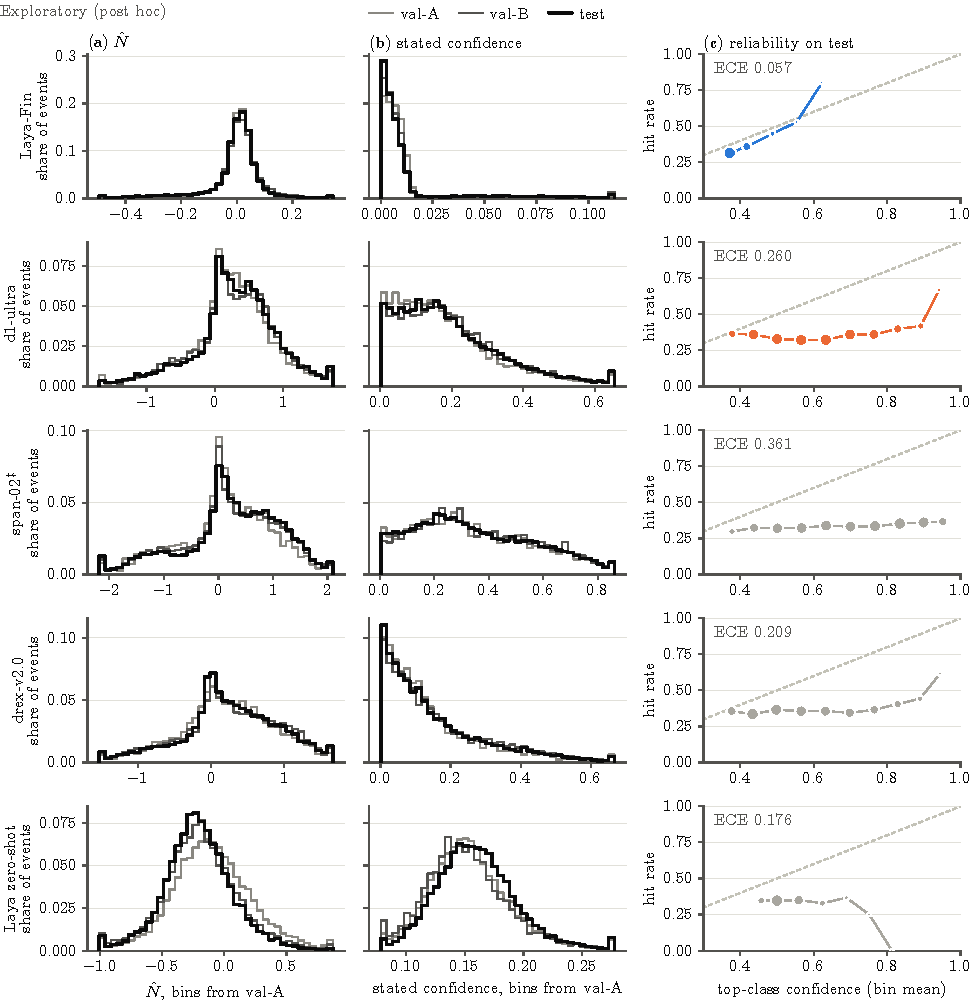
\includegraphics{figA19_output_histograms.pdf}
\caption{\textbf{Exploratory (post hoc): the decision models' outputs beside their reliability.} Exploratory (post hoc): NA-13b, requested after unblinding; no hypothesis, no claim. Its thresholds, medians and bins come from val-A, and the test was evaluated once. For each model, the share of its D0 events in each of 40 bins of (a) $\hat N$ and (b) the stated confidence, $1 - H/\log 3$ of Q1's three classes (the measure of the frozen gates), on val-A, val-B and the test; the bins span the val-A 0.5th to 99.5th percentiles and the end bins hold the values beyond. (c) NA-12's reliability diagram on the test (Figure A4): the hit rate of Q1's top class against $e_5$ by bin of the top-class probability, the confidence of \S{}11.2's ECE, not the entropy confidence of (b); dot area grows with the events in the bin, the dashed diagonal is perfect calibration. Laya-Fin reads small: its $\hat N$ has an SD of 0.11 on test against 0.61 for d1-ultra, and its stated confidence stays below 0.073 for 95\% of its test events; it is calibrated (ECE 0.057) where d1-ultra is not (0.260). The distributions barely move from val-A to the test, except Laya zero-shot's $\hat N$ (median $-$0.11 on val-A, $-$0.21 on test). span-02's and drex-v2.0's val-A histograms come from NA-06's 3,000-event stage-2 sample. $\ddagger$ span-02: the S5 canary fired a STOP after the freeze and the operator chose to proceed (PREREG \S{}15).}\label{fig:figA19_output_histograms}
\end{figure}

\clearpage

% t36_selective_coverage: tab:a-selective-coverage (NA-14 figures.latex, from artifacts/NA-14/tables/t36_selective_coverage.csv)
\begin{table}[htbp]
\centering
\small
\setlength{\tabcolsep}{4pt}
\begin{threeparttable}
\caption{Exploratory (post hoc): ranking by conviction concentrates the overnight move, which the open prices; the move after the open stays within its 95\% interval of zero at every coverage on the test (NA-13b).}\label{tab:a-selective-coverage}
\begin{tabular}{@{}lS[table-format=1.3]S[table-format=1.3]S[table-format=1.3]S[table-format=1.3]S[table-format=1.3]S[table-format=1.3]S[table-format=1.3]S[table-format=1.3]S[table-format=1.3]@{}}
\toprule
 & \multicolumn{3}{c}{val-A} & \multicolumn{3}{c}{val-B} & \multicolumn{3}{c}{Test} \\
\cmidrule(lr){2-4}\cmidrule(lr){5-7}\cmidrule(lr){8-10}
Model, coverage & {$z_{cc}$} & {$z_{on}$} & {$z_{id}$} & {$z_{cc}$} & {$z_{on}$} & {$z_{id}$} & {$z_{cc}$} & {$z_{on}$} & {$z_{id}$} \\
\midrule
\multicolumn{10}{@{}l}{\textit{Panel A: mean signed move $\mathrm{sign}(\hat N)\,z$ (typical daily moves)}} \\
Laya-Fin, 100\% & 0.088 & 0.064 & 0.058 & 0.083 & 0.093 & 0.037 & 0.043 & 0.063 & 0.016 \\
Laya-Fin, 30\% & 0.231 & 0.265 & 0.086 & 0.183 & 0.137 & 0.114 & 0.083 & 0.136 & 0.024 \\
Laya-Fin, 10\% & 0.459 & 0.569 & 0.106 & 0.351 & 0.332 & 0.123 & 0.172 & 0.191 & 0.068 \\
d1-ultra, 100\% & 0.133 & 0.223 & 0.025 & 0.155 & 0.259 & 0.022 & 0.102 & 0.212 & 0.005 \\
d1-ultra, 30\% & 0.366 & 0.677 & 0.034 & 0.369 & 0.604 & 0.053 & 0.273 & 0.508 & 0.025 \\
d1-ultra, 10\% & 0.799 & 1.516 & 0.004 & 0.754 & 1.157 & 0.140 & 0.592 & 0.930 & 0.101 \\
\addlinespace
\multicolumn{10}{@{}l}{\textit{Panel B: hit rate, the share with $\mathrm{sign}(\hat N) = \mathrm{sign}(z)$}} \\
Laya-Fin, 100\% & 0.518 & 0.498 & 0.516 & 0.512 & 0.513 & 0.511 & 0.509 & 0.505 & 0.505 \\
Laya-Fin, 30\% & 0.544 & 0.517 & 0.522 & 0.528 & 0.527 & 0.527 & 0.515 & 0.519 & 0.501 \\
Laya-Fin, 10\% & 0.562 & 0.500 & 0.520 & 0.542 & 0.542 & 0.539 & 0.526 & 0.525 & 0.510 \\
d1-ultra, 100\% & 0.524 & 0.521 & 0.514 & 0.520 & 0.523 & 0.507 & 0.506 & 0.524 & 0.501 \\
d1-ultra, 30\% & 0.550 & 0.575 & 0.515 & 0.539 & 0.535 & 0.504 & 0.521 & 0.553 & 0.502 \\
d1-ultra, 10\% & 0.587 & 0.616 & 0.501 & 0.566 & 0.577 & 0.517 & 0.556 & 0.587 & 0.523 \\
\bottomrule
\end{tabular}
\begin{tablenotes}[flushleft]\footnotesize
\item Exploratory (post hoc): requested after unblinding; no hypothesis, outside every family, no claim. NA-13b, the operator's study of when the D0 signal works (PREREG \S15, NA-13b row): thresholds from val-A. The operator's assistant computed the first of these statistics on all three splits, the test included, before NA-13b (the band check of Table~\ref{tab:a-band-disclosure} and the first four ICs of Table~\ref{tab:a-watch-open}); they shaped the study, they are reproduced exactly here, and no threshold is chosen from them.
\item Coverage: the D0 events whose conviction $|\hat N|$ is at or above its val-A quantile at one minus the coverage (100\%: every event); events outside the embargo; moves in typical daily moves. The 95\% intervals (stationary block bootstrap), every coverage, the other models and the ranking by the stated confidence are in the table's CSV and Figure A16; the daily IC inside the covered set is in the CSV only.
\item The API models fail the \S8.3 contamination screens, so their results are model-specific (\S1.3).
\end{tablenotes}
\end{threeparttable}
\end{table}


\clearpage

% t37_watch_open: tab:a-watch-open (NA-14 figures.latex, from artifacts/NA-14/tables/t37_watch_open.csv, artifacts/NA-12/tables/t2_h2_over_under.csv, artifacts/NA-12/tables/t6_convergence_ladder.csv, artifacts/NA-12/tables/t7_gap_closure.csv, artifacts/NA-14/tables/t20_strategies.csv)
\begin{table}[htbp]
\centering
\small
\setlength{\tabcolsep}{4pt}
\begin{threeparttable}
\caption{Exploratory (post hoc): the 10:00 reading adds nothing to the pre-open one; on val-B and the test the ICs of the 10:00 reading and of the revision with $y_1$ are negative for both models (NA-13b).}\label{tab:a-watch-open}
\begin{tabular}{@{}>{\raggedright\arraybackslash}p{2.95in}S[table-format=-1.3]S[table-format=-1.2]S[table-format=-1.3]S[table-format=-1.2]S[table-format=-1.3]S[table-format=-1.2]@{}}
\toprule
 & \multicolumn{2}{c}{val-A} & \multicolumn{2}{c}{val-B} & \multicolumn{2}{c}{Test} \\
\cmidrule(lr){2-3}\cmidrule(lr){4-5}\cmidrule(lr){6-7}
Model: statistic & {Value} & {$t$} & {Value} & {$t$} & {Value} & {$t$} \\
\midrule
\multicolumn{7}{@{}l}{\textit{Panel A: watching the open (NA-13b)}} \\
Laya-Fin: IC, pre-open reading $\hat N_{\mathrm{D0}}$ & 0.047 & 3.94 & 0.008 & 0.50 & 0.026 & 2.09 \\
Laya-Fin: IC, 10:00 reading $\hat N_{\mathrm{D1}}$ & 0.034 & 1.66 & -0.024 & -1.48 & -0.013 & -0.85 \\
Laya-Fin: IC, the revision & 0.001 & 0.07 & -0.027 & -1.41 & -0.036 & -2.33 \\
Laya-Fin: IC, the first bar $G_{\mathrm{D1}}$ & 0.030 & 1.53 & -0.034 & -1.59 & -0.016 & -1.03 \\
Laya-Fin: mean, first bar against & -0.010 & -0.35 & 0.000 & -0.01 & 0.045 & 1.73 \\
Laya-Fin: mean, first bar with & 0.111 & 3.74 & -0.037 & -1.18 & -0.001 & -0.04 \\
d1-ultra: IC, pre-open reading $\hat N_{\mathrm{D0}}$ & 0.014 & 0.90 & 0.019 & 1.64 & -0.004 & -0.31 \\
d1-ultra: IC, 10:00 reading $\hat N_{\mathrm{D1}}$ & 0.029 & 1.41 & -0.020 & -1.52 & -0.014 & -1.11 \\
d1-ultra: IC, the revision & 0.018 & 1.21 & -0.043 & -2.68 & -0.011 & -0.84 \\
d1-ultra: IC, the first bar $G_{\mathrm{D1}}$ & 0.030 & 1.53 & -0.034 & -1.59 & -0.016 & -1.03 \\
d1-ultra: mean, first bar against & -0.039 & -1.52 & 0.039 & 1.32 & 0.008 & 0.35 \\
d1-ultra: mean, first bar with & 0.078 & 3.15 & -0.013 & -0.38 & -0.036 & -1.50 \\
\addlinespace
\multicolumn{7}{@{}l}{\textit{Panel B: pre-registered D1 results (NA-12, NA-13; test, for reference)}} \\
Laya-Fin: over/under $b$ at D1 & {---} & {---} & {---} & {---} & 0.229 & {---} \\
Laya-Fin: over/under $c$ at D1 & {---} & {---} & {---} & {---} & 0.013 & {---} \\
Laya-Fin: $\kappa$ at 10:00 & {---} & {---} & {---} & {---} & 0.273 & {---} \\
Laya-Fin: $\lambda$ at $C_t$ from D1 & {---} & {---} & {---} & {---} & -0.011 & {---} \\
Laya-Fin: S-D1 $J$, gross Sharpe & {---} & {---} & {---} & {---} & 0.76 & {---} \\
Laya-Fin: S-CONV from 10:00, gross Sharpe & {---} & {---} & {---} & {---} & 1.61 & {---} \\
d1-ultra: over/under $b$ at D1 & {---} & {---} & {---} & {---} & -0.018 & {---} \\
d1-ultra: over/under $c$ at D1 & {---} & {---} & {---} & {---} & 0.015 & {---} \\
d1-ultra: $\kappa$ at 10:00 & {---} & {---} & {---} & {---} & 0.610 & {---} \\
d1-ultra: $\lambda$ at $C_t$ from D1 & {---} & {---} & {---} & {---} & -0.013 & {---} \\
d1-ultra: S-D1 $J$, gross Sharpe & {---} & {---} & {---} & {---} & -0.28 & {---} \\
d1-ultra: S-CONV from 10:00, gross Sharpe & {---} & {---} & {---} & {---} & 0.03 & {---} \\
\bottomrule
\end{tabular}
\begin{tablenotes}[flushleft]\footnotesize
\item Exploratory (post hoc): requested after unblinding; no hypothesis, outside every family, no claim. NA-13b, the operator's study of when the D0 signal works (PREREG \S15, NA-13b row): thresholds and medians from val-A, the conditions selected on val-A and val-B by a rule fixed before the test, the test evaluated once.
\item Panel A: the daily IC with $y_1$, the move from 10:00 to the close (PREREG \S5.6), of the pre-open reading $\hat N_{\mathrm{D0}}$, of the 10:00 reading $\hat N_{\mathrm{D1}}$ (Call B at D1), of the revision $z(\hat N_{\mathrm{D1}}) - z(\hat N_{\mathrm{D0}})$ and of the first bar's move $G_{\mathrm{D1}}$, with its Newey--West $t$ (5 lags); then the mean of $\mathrm{sign}(\hat N_{\mathrm{D0}})\,y_1$ over the events whose first bar moved against, or with, the pre-open reading, with a day-clustered $t$. Events outside the embargo; the first bar is the same for both models.
\item Panel B: the pre-registered D1 estimates on the test (NA-12, NA-13): the over/under coefficients $b$ and $c$ (Table~\ref{tab:a-h2-over-under}), $\kappa$ at 10:00 (Table~\ref{tab:a-convergence-ladder}), $\lambda$ at the close from D1 (Table~\ref{tab:a-gap-closure}) and the annualized gross Sharpe ratios of S-D1 $J$ and of S-CONV from 10:00 to the close (Table~\ref{tab:a-strategies}). ---: Panel B holds the test estimates only; their standard errors and $p$ are in those tables.
\item The API models fail the \S8.3 contamination screens, so their results are model-specific (\S1.3).
\end{tablenotes}
\end{threeparttable}
\end{table}


\clearpage

% t38_conditioning: tab:a-conditioning (NA-14 figures.latex, from artifacts/NA-14/tables/t38_conditioning.csv)
\begin{landscape}
\begingroup
\footnotesize
\setlength{\tabcolsep}{4pt}
\begin{longtable}{@{}>{\raggedright\arraybackslash}p{2.7in}S[table-format=-1.3]S[table-format=-1.2]S[table-format=-1.3]S[table-format=-1.2]S[table-format=-1.2]cS[table-format=-1.3]S[table-format=-1.2]S[table-format=1.3]S[table-format=1.3]c@{}}
\caption{Exploratory (post hoc): the conditioning study; none of the pairs selected on validation held on the test, and no pair of the family is confirmed (NA-13b).}\label{tab:a-conditioning} \\
\toprule
 & \multicolumn{2}{c}{val-A} & \multicolumn{2}{c}{val-B} & \multicolumn{2}{c}{Validation} & \multicolumn{5}{c}{Test, evaluated once} \\
\cmidrule(lr){2-3}\cmidrule(lr){4-5}\cmidrule(lr){6-7}\cmidrule(lr){8-12}
Condition & {Diff.} & {$t$} & {Diff.} & {$t$} & {Pooled $t$} & Selected & {Diff.} & {$t$} & {BH $q$} & {BH $q$, unseen} & Confirmed \\
\midrule
\endfirsthead
\multicolumn{12}{@{}l}{\textit{Table \ref{tab:a-conditioning}, continued (Laya-Fin)}} \\
\toprule
 & \multicolumn{2}{c}{val-A} & \multicolumn{2}{c}{val-B} & \multicolumn{2}{c}{Validation} & \multicolumn{5}{c}{Test, evaluated once} \\
\cmidrule(lr){2-3}\cmidrule(lr){4-5}\cmidrule(lr){6-7}\cmidrule(lr){8-12}
Condition & {Diff.} & {$t$} & {Diff.} & {$t$} & {Pooled $t$} & Selected & {Diff.} & {$t$} & {BH $q$} & {BH $q$, unseen} & Confirmed \\
\midrule
\endhead
\midrule
\multicolumn{12}{r@{}}{\textit{continued on the next page}} \\
\endfoot
\bottomrule
\endlastfoot
\multicolumn{12}{@{}l}{\textit{Laya-Fin}} \\
E1 earnings day [seen on test] & 0.225 & 0.72 & 0.167 & 0.50 & 0.87 & no & -0.330 & -1.58 & 0.935 & {---} & no \\
E1 quantified$^{\dagger}$ & -0.006 & -0.17 & -0.098 & -1.18 & -1.16 & no & -0.008 & -0.15 & 0.935 & 0.924 & no \\
E1 press wire$^{\dagger}$ & 0.020 & 0.57 & 0.008 & 0.15 & 0.46 & no & -0.013 & -0.45 & 0.935 & 0.924 & no \\
E1 imprecise timestamp$^{\dagger}$ & -0.012 & -0.32 & 0.008 & 0.11 & -0.04 & no & -0.060 & -1.26 & 0.935 & 0.924 & no \\
E2 new, not known & 0.033 & 0.82 & 0.055 & 1.18 & 1.43 & no & 0.024 & 0.85 & 0.935 & 0.924 & no \\
E2 numbers, not narrative & 0.061 & 1.63 & 0.150 & 2.96 & 3.34 & yes & -0.040 & -0.98 & 0.935 & 0.924 & no \\
E2 scheduled & 0.032 & 1.03 & 0.012 & 0.25 & 0.77 & no & -0.008 & -0.26 & 0.935 & 0.924 & no \\
E2 company-specific & 0.027 & 0.70 & 0.164 & 1.95 & 2.05 & no & -0.024 & -0.41 & 0.935 & 0.924 & no \\
E2 confirmed & -0.012 & -0.35 & 0.136 & 2.83 & 2.04 & no & -0.007 & -0.23 & 0.935 & 0.924 & no \\
E2 impact horizon above median & -0.020 & -0.56 & -0.007 & -0.18 & -0.51 & no & 0.033 & 1.15 & 0.935 & 0.924 & no \\
E2 uncertainty below median & -0.015 & -0.51 & -0.139 & -3.37 & -2.98 & no & 0.014 & 0.43 & 0.935 & 0.924 & no \\
E2 mixed signals below median & 0.016 & 0.39 & -0.008 & -0.14 & 0.11 & no & -0.067 & -2.20 & 0.935 & 0.924 & no \\
E2 materiality above median & 0.074 & 2.31 & 0.088 & 2.49 & 3.40 & yes & -0.016 & -0.49 & 0.935 & 0.924 & no \\
E2 $P$(no material effect) below median & 0.073 & 2.61 & 0.079 & 2.02 & 3.17 & yes & -0.037 & -1.20 & 0.935 & 0.924 & no \\
E3 latest article before 08:00 [seen on test] & -0.018 & -0.51 & -0.102 & -1.85 & -1.83 & no & 0.018 & 0.54 & 0.935 & {---} & no \\
E3 04:00 to 08:00, not 08:00 to 09:15 & -0.022 & -0.55 & -0.105 & -1.66 & -1.69 & no & 0.030 & 0.79 & 0.935 & 0.924 & no \\
E4 Friday & 0.021 & 0.35 & -0.075 & -1.46 & -0.67 & no & -0.007 & -0.15 & 0.935 & 0.924 & no \\
E4 Monday & -0.003 & -0.07 & 0.034 & 0.70 & 0.48 & no & -0.008 & -0.20 & 0.935 & 0.924 & no \\
E4 busy news day (ratio $\geq 1.5$) & 0.046 & 1.17 & 0.191 & 2.51 & 2.75 & yes & 0.014 & 0.40 & 0.935 & 0.924 & no \\
E4 news count above median & 0.058 & 1.33 & -0.004 & -0.08 & 1.06 & no & 0.029 & 0.87 & 0.935 & 0.924 & no \\
E4 earnings count above median & 0.090 & 2.18 & 0.015 & 0.33 & 1.65 & no & -0.007 & -0.20 & 0.935 & 0.924 & no \\
E4 FOMC, CPI or payrolls day & 0.052 & 0.54 & 0.096 & 1.04 & 1.14 & no & -0.062 & -1.06 & 0.935 & 0.924 & no \\
E4 VIX at $t-1$ above median & 0.006 & 0.14 & -0.001 & -0.01 & -0.10 & no & 0.114 & 1.50 & 0.935 & 0.924 & no \\
E4 $|$SPY overnight$|$ above median & 0.012 & 0.28 & 0.028 & 0.61 & 0.59 & no & -0.008 & -0.23 & 0.935 & 0.924 & no \\
E5 size tier 251 to 500 & -0.001 & -0.02 & 0.091 & 1.74 & 1.49 & no & -0.007 & -0.23 & 0.935 & 0.924 & no \\
E5 dollar-volume tier 251 to 500 & -0.040 & -1.10 & 0.037 & 0.64 & -0.04 & no & -0.013 & -0.44 & 0.935 & 0.924 & no \\
E5 low usual coverage & 0.043 & 1.32 & 0.058 & 0.97 & 1.50 & no & 0.021 & 0.35 & 0.935 & 0.924 & no \\
E5 $\sigma$ above median & 0.003 & 0.11 & 0.018 & 0.43 & 0.42 & no & 0.047 & 1.30 & 0.935 & 0.924 & no \\
E5 direction agrees with $z_{m20}$ & 0.025 & 0.56 & 0.001 & 0.02 & 0.35 & no & -0.006 & -0.13 & 0.935 & 0.924 & no \\
E5 price-move text & -0.003 & -0.05 & 0.011 & 0.14 & 0.08 & no & 0.045 & 0.82 & 0.935 & 0.924 & no \\
E6 conviction top 30\% [seen on test] & 0.038 & 0.77 & 0.127 & 2.55 & 2.35 & no & 0.004 & 0.09 & 0.942 & {---} & no \\
E6 Laya-Fin's magnitude above median & 0.057 & 1.68 & 0.120 & 2.79 & 3.22 & yes & -0.016 & -0.48 & 0.935 & 0.924 & no \\
E6 d1-ultra's confidence above median & 0.019 & 0.55 & -0.014 & -0.31 & 0.09 & no & -0.049 & -1.73 & 0.935 & 0.924 & no \\
E7 Laya-Fin and d1-ultra agree & 0.003 & 0.06 & -0.028 & -0.52 & -0.37 & no & -0.016 & -0.50 & 0.935 & 0.924 & no \\
E7 three API models agree & {---} & {---} & 0.086 & 1.65 & {---} & no & -0.020 & -0.53 & 0.935 & 0.924 & no \\
E7 rank average of the two models & -0.028 & -1.96 & -0.010 & -0.61 & -1.74 & no & -0.001 & -0.04 & 0.966 & 0.966 & no \\
E8 $|V|\,\sigma$ above the hurdle & 0.097 & 0.91 & 0.182 & 1.63 & 1.79 & no & 0.051 & 0.73 & 0.935 & 0.924 & no \\
E9 numbers and material & 0.074 & 1.44 & 0.208 & 3.40 & 3.51 & yes & -0.058 & -1.00 & 0.935 & 0.924 & no \\
\end{longtable}
\begin{longtable}{@{}>{\raggedright\arraybackslash}p{2.7in}S[table-format=-1.3]S[table-format=-1.2]S[table-format=-1.3]S[table-format=-1.2]S[table-format=-1.2]cS[table-format=-1.3]S[table-format=-1.2]S[table-format=1.3]S[table-format=1.3]c@{}}
\multicolumn{12}{@{}l}{\textit{Table \ref{tab:a-conditioning}, continued (d1-ultra)}} \\
\toprule
 & \multicolumn{2}{c}{val-A} & \multicolumn{2}{c}{val-B} & \multicolumn{2}{c}{Validation} & \multicolumn{5}{c}{Test, evaluated once} \\
\cmidrule(lr){2-3}\cmidrule(lr){4-5}\cmidrule(lr){6-7}\cmidrule(lr){8-12}
Condition & {Diff.} & {$t$} & {Diff.} & {$t$} & {Pooled $t$} & Selected & {Diff.} & {$t$} & {BH $q$} & {BH $q$, unseen} & Confirmed \\
\midrule
\endfirsthead
\multicolumn{12}{@{}l}{\textit{Table \ref{tab:a-conditioning}, continued (d1-ultra)}} \\
\toprule
 & \multicolumn{2}{c}{val-A} & \multicolumn{2}{c}{val-B} & \multicolumn{2}{c}{Validation} & \multicolumn{5}{c}{Test, evaluated once} \\
\cmidrule(lr){2-3}\cmidrule(lr){4-5}\cmidrule(lr){6-7}\cmidrule(lr){8-12}
Condition & {Diff.} & {$t$} & {Diff.} & {$t$} & {Pooled $t$} & Selected & {Diff.} & {$t$} & {BH $q$} & {BH $q$, unseen} & Confirmed \\
\midrule
\endhead
\midrule
\multicolumn{12}{r@{}}{\textit{continued on the next page}} \\
\endfoot
\bottomrule
\endlastfoot
\multicolumn{12}{@{}l}{\textit{d1-ultra}} \\
E1 earnings day [seen on test] & -0.173 & -0.56 & -0.125 & -0.36 & -0.65 & no & 0.268 & 1.33 & 0.935 & {---} & no \\
E1 quantified$^{\dagger}$ & -0.063 & -1.55 & -0.062 & -0.80 & -1.43 & no & 0.012 & 0.23 & 0.935 & 0.924 & no \\
E1 press wire$^{\dagger}$ & 0.054 & 1.41 & -0.058 & -1.40 & -0.07 & no & -0.016 & -0.49 & 0.935 & 0.924 & no \\
E1 imprecise timestamp$^{\dagger}$ & -0.025 & -0.64 & -0.129 & -1.82 & -1.89 & no & -0.014 & -0.32 & 0.935 & 0.924 & no \\
E2 new, not known & 0.070 & 1.57 & -0.063 & -1.60 & 0.10 & no & 0.047 & 1.58 & 0.935 & 0.924 & no \\
E2 numbers, not narrative & 0.056 & 1.34 & 0.022 & 0.42 & 1.16 & no & 0.033 & 0.75 & 0.935 & 0.924 & no \\
E2 scheduled & 0.004 & 0.13 & -0.011 & -0.23 & -0.12 & no & -0.021 & -0.66 & 0.935 & 0.924 & no \\
E2 company-specific & -0.004 & -0.11 & 0.066 & 0.85 & 0.74 & no & -0.103 & -1.60 & 0.935 & 0.924 & no \\
E2 confirmed & 0.059 & 1.58 & 0.038 & 0.90 & 1.73 & no & 0.027 & 0.94 & 0.935 & 0.924 & no \\
E2 impact horizon above median & 0.010 & 0.28 & 0.025 & 0.51 & 0.59 & no & -0.021 & -0.60 & 0.935 & 0.924 & no \\
E2 uncertainty below median & -0.065 & -1.61 & -0.052 & -1.33 & -2.09 & no & 0.005 & 0.15 & 0.935 & 0.924 & no \\
E2 mixed signals below median & -0.037 & -0.86 & 0.078 & 1.41 & 0.59 & no & 0.055 & 1.60 & 0.935 & 0.924 & no \\
E2 materiality above median & 0.040 & 1.29 & 0.037 & 0.92 & 1.53 & no & 0.023 & 0.69 & 0.935 & 0.924 & no \\
E2 $P$(no material effect) below median & 0.062 & 1.67 & 0.040 & 0.97 & 1.85 & no & -0.012 & -0.39 & 0.935 & 0.924 & no \\
E3 latest article before 08:00 [seen on test] & 0.002 & 0.05 & 0.018 & 0.38 & 0.34 & no & 0.029 & 0.81 & 0.935 & {---} & no \\
E3 04:00 to 08:00, not 08:00 to 09:15 & 0.038 & 0.92 & 0.048 & 0.90 & 1.28 & no & 0.012 & 0.29 & 0.935 & 0.924 & no \\
E4 Friday & -0.018 & -0.44 & -0.142 & -2.50 & -2.19 & no & -0.034 & -1.08 & 0.935 & 0.924 & no \\
E4 Monday & 0.026 & 0.59 & 0.047 & 0.98 & 1.13 & no & -0.006 & -0.20 & 0.935 & 0.924 & no \\
E4 busy news day (ratio $\geq 1.5$) & -0.040 & -0.94 & -0.095 & -1.31 & -1.61 & no & -0.014 & -0.38 & 0.935 & 0.924 & no \\
E4 news count above median & 0.042 & 1.13 & 0.102 & 1.82 & 2.31 & yes & 0.021 & 0.65 & 0.935 & 0.924 & no \\
E4 earnings count above median & 0.022 & 0.61 & -0.010 & -0.20 & 0.14 & no & 0.031 & 1.06 & 0.935 & 0.924 & no \\
E4 FOMC, CPI or payrolls day & -0.053 & -0.69 & -0.054 & -1.04 & -1.14 & no & 0.052 & 1.03 & 0.935 & 0.924 & no \\
E4 VIX at $t-1$ above median & 0.016 & 0.42 & -0.024 & -0.47 & -0.22 & no & 0.135 & 3.11 & 0.790 & 0.727 & no \\
E4 $|$SPY overnight$|$ above median & 0.029 & 0.78 & -0.051 & -1.06 & -0.40 & no & 0.007 & 0.24 & 0.935 & 0.924 & no \\
E5 size tier 251 to 500 & -0.018 & -0.42 & -0.056 & -1.31 & -1.24 & no & -0.005 & -0.16 & 0.935 & 0.924 & no \\
E5 dollar-volume tier 251 to 500 & -0.079 & -2.10 & -0.055 & -0.99 & -2.01 & no & -0.003 & -0.10 & 0.942 & 0.933 & no \\
E5 low usual coverage & -0.074 & -1.90 & -0.048 & -0.90 & -1.85 & no & -0.030 & -0.46 & 0.935 & 0.924 & no \\
E5 $\sigma$ above median & 0.056 & 1.72 & 0.011 & 0.22 & 1.15 & no & 0.016 & 0.43 & 0.935 & 0.924 & no \\
E5 direction agrees with $z_{m20}$ & 0.039 & 0.85 & 0.018 & 0.30 & 0.76 & no & -0.007 & -0.17 & 0.935 & 0.924 & no \\
E5 price-move text & -0.013 & -0.25 & -0.013 & -0.15 & -0.26 & no & -0.057 & -1.10 & 0.935 & 0.924 & no \\
E6 conviction top 30\% [seen on test] & 0.007 & 0.13 & 0.082 & 1.74 & 1.22 & no & 0.023 & 0.60 & 0.935 & {---} & no \\
E6 Laya-Fin's magnitude above median & 0.052 & 1.56 & 0.049 & 1.05 & 1.78 & no & -0.016 & -0.46 & 0.935 & 0.924 & no \\
E6 d1-ultra's confidence above median & -0.055 & -1.36 & 0.027 & 0.66 & -0.49 & no & 0.010 & 0.33 & 0.935 & 0.924 & no \\
E7 Laya-Fin and d1-ultra agree & 0.101 & 2.02 & 0.073 & 1.45 & 2.46 & yes & 0.039 & 1.01 & 0.935 & 0.924 & no \\
E7 three API models agree & {---} & {---} & -0.015 & -0.30 & {---} & no & 0.029 & 0.81 & 0.935 & 0.924 & no \\
E7 rank average of the two models & 0.001 & 0.08 & 0.025 & 1.16 & 0.98 & no & 0.016 & 1.00 & 0.935 & 0.924 & no \\
E8 $|V|\,\sigma$ above the hurdle & 0.013 & 0.19 & 0.193 & 2.90 & 2.15 & no & 0.060 & 1.24 & 0.935 & 0.924 & no \\
\end{longtable}
\endgroup
\vspace{-0.5\baselineskip}
{\footnotesize\raggedright
Exploratory (post hoc): requested after unblinding; no hypothesis, outside every family, no claim. NA-13b, the operator's study of when the D0 signal works (PREREG \S15, NA-13b row): thresholds and medians from val-A, the conditions selected on val-A and val-B by a rule fixed before the test, the test evaluated once.\par
Diff.: the inside-minus-outside difference of the primary outcome $\mathrm{sign}(\hat N)\,z_{id}$ (typical daily moves): at the event level the mean of the daily differences with a day-clustered $t$; at the day level (Friday, Monday, the day's news and earnings counts, macro days, VIX, SPY's overnight move) the difference of the sessions' means with Welch's $t$; for the rank average the mean daily difference to the model's own sign. Selected on validation by the operator's rule, fixed before the test: positive with $t \geq 1$ in val-A and in val-B and a pooled $t \geq 2$ (the three-model agreement: val-B alone, $t \geq 2.5$). The test, once: two-sided $p$, Benjamini--Hochberg at $q = 0.10$ over the family and over the family without the conditions seen on test (unseen); confirmed: selected, the same sign on the test and BH $q < 0.10$.\par
[seen on test]: earnings day, latest article before 08:00 and conviction top 30\%, which the test had shown before this study; reported, never selected. $^{\dagger}$Vendor field: a label the vendor produced retrospectively, possibly look-ahead-contaminated. ---: the three-model agreement has no val-A run (span-02 and drex-v2.0 have no val-A production run), so no pooled $t$; a condition seen on test has no unseen $q$.\par
The API models fail the pre-registered contamination screens, so their results are model-specific.\par
}
\end{landscape}


\clearpage

% t39_conditioning_books: tab:a-conditioning-books (NA-14 figures.latex, from artifacts/NA-14/tables/t39_conditioning_books.csv)
\begin{table}[htbp]
\centering
\footnotesize
\setlength{\tabcolsep}{4pt}\renewcommand{\arraystretch}{0.92}
\begin{threeparttable}
\caption{Exploratory (post hoc): the tradable versions; on the test none beats its placebo (NA-13b).}\label{tab:a-conditioning-books}
\begin{tabular}{@{}llS[table-format=-1.2]S[table-format=-1.2]S[table-format=-1.2]S[table-format=-2.1]S[table-format=3.1]S[table-format=2.1]S[table-format=3.0]S[table-format=1.3, table-space-text-pre={$<$}]@{}}
\toprule
 & & \multicolumn{3}{c}{Sharpe ratio} & & \multicolumn{2}{c}{Names} & & \\
\cmidrule(lr){3-5}\cmidrule(lr){7-8}
Book & Exit & {Gross} & {5 bp} & {10 bp} & {Break-even} & {Long} & {Short} & {Placebo} & {DSR} \\
\midrule
\multicolumn{10}{@{}l}{\textit{Test: Laya-Fin}} \\
E2 numbers, not narrative & $C_t$ & -0.73 & -3.15 & -5.54 & -1.5 & 17.4 & 14.1 & 41 & {$<$}0.001 \\
 & $t{+}1$ & -1.62 & -3.13 & -4.63 & -5.3 & 17.4 & 14.1 & 15 & {$<$}0.001 \\
E2 materiality above median & $C_t$ & 0.19 & -3.24 & -6.63 & 0.3 & 22.7 & 19.9 & 66 & {$<$}0.001 \\
 & $t{+}1$ & -1.29 & -3.42 & -5.55 & -3.0 & 22.7 & 19.9 & 14 & {$<$}0.001 \\
E2 $P$(no material effect) below median & $C_t$ & -0.57 & -3.93 & -7.27 & -0.8 & 30.3 & 24.7 & 38 & {$<$}0.001 \\
 & $t{+}1$ & -1.24 & -3.34 & -5.42 & -3.0 & 30.3 & 24.7 & 18 & {$<$}0.001 \\
E4 busy news day (ratio $\geq 1.5$) & $C_t$ & 0.35 & -2.77 & -5.88 & 0.6 & 30.2 & 23.7 & 64 & {$<$}0.001 \\
 & $t{+}1$ & -0.86 & -2.47 & -4.07 & -2.7 & 30.2 & 23.7 & 28 & {$<$}0.001 \\
E6 Laya-Fin's magnitude above median & $C_t$ & 0.67 & -2.75 & -6.15 & 1.0 & 33.0 & 28.6 & 67 & {$<$}0.001 \\
 & $t{+}1$ & -0.52 & -2.44 & -4.35 & -1.4 & 33.0 & 28.6 & 37 & {$<$}0.001 \\
E9 numbers and material & $C_t$ & -0.71 & -2.45 & -4.18 & -2.0 & 10.7 & 11.2 & 31 & {$<$}0.001 \\
 & $t{+}1$ & -2.38 & -3.58 & -4.77 & -9.8 & 10.7 & 11.2 & 5 & {$<$}0.001 \\
E8 $|V|\,\sigma$ above the hurdle & $C_t$ & 0.88 & -0.38 & -1.63 & 3.5 & 4.9 & 7.3 & 73 & {$<$}0.001 \\
 & $t{+}1$ & 1.47 & 0.74 & 0.01 & 10.0 & 4.9 & 7.3 & 85 & {$<$}0.001 \\
\addlinespace
\multicolumn{10}{@{}l}{\textit{Test: d1-ultra}} \\
E4 news count above median & $C_t$ & 0.36 & -2.81 & -5.25 & 0.5 & 133.9 & 37.4 & 60 & {$<$}0.001 \\
 & $t{+}1$ & 0.82 & -1.20 & -3.17 & 2.0 & 133.9 & 37.4 & 77 & {$<$}0.001 \\
E7 Laya-Fin and d1-ultra agree & $C_t$ & 0.62 & -2.84 & -6.32 & 0.9 & 48.2 & 14.7 & 66 & {$<$}0.001 \\
 & $t{+}1$ & -0.49 & -2.39 & -4.30 & -1.3 & 48.2 & 14.7 & 30 & {$<$}0.001 \\
E8 $|V|\,\sigma$ above the hurdle & $C_t$ & 0.05 & -1.66 & -3.36 & 0.2 & 11.8 & 8.2 & 54 & {$<$}0.001 \\
 & $t{+}1$ & -0.70 & -1.83 & -2.95 & -3.1 & 11.8 & 8.2 & 30 & {$<$}0.001 \\
\addlinespace
\multicolumn{10}{@{}l}{\textit{Val-B, in-sample for the selection: Laya-Fin}} \\
E2 numbers, not narrative & $C_t$ & 5.43 & 2.52 & -0.44 & 9.3 & 18.2 & 13.2 & 100 & {$<$}0.001 \\
 & $t{+}1$ & 4.00 & 1.87 & -0.26 & 9.4 & 18.2 & 13.2 & 97 & {$<$}0.001 \\
E2 materiality above median & $C_t$ & 5.50 & 0.69 & -4.13 & 5.7 & 24.9 & 20.0 & 100 & {$<$}0.001 \\
 & $t{+}1$ & 2.83 & -0.27 & -3.37 & 4.6 & 25.3 & 20.3 & 88 & {$<$}0.001 \\
E2 $P$(no material effect) below median & $C_t$ & 4.60 & -0.14 & -4.86 & 4.8 & 29.2 & 21.4 & 98 & {$<$}0.001 \\
 & $t{+}1$ & 4.44 & 1.12 & -2.19 & 6.7 & 29.2 & 21.4 & 98 & {$<$}0.001 \\
E4 busy news day (ratio $\geq 1.5$) & $C_t$ & 5.99 & 3.44 & 0.84 & 11.6 & 16.8 & 12.6 & 100 & 0.001 \\
 & $t{+}1$ & 5.05 & 3.46 & 1.85 & 15.7 & 16.8 & 12.6 & 100 & 0.005 \\
E6 Laya-Fin's magnitude above median & $C_t$ & 5.56 & 0.65 & -4.29 & 5.7 & 32.8 & 25.7 & 100 & {$<$}0.001 \\
 & $t{+}1$ & 3.41 & 0.38 & -2.65 & 5.6 & 33.4 & 26.1 & 94 & {$<$}0.001 \\
E9 numbers and material & $C_t$ & 6.78 & 4.23 & 1.65 & 13.2 & 12.8 & 11.1 & 100 & 0.004 \\
 & $t{+}1$ & 4.12 & 2.27 & 0.41 & 11.1 & 12.8 & 11.1 & 98 & {$<$}0.001 \\
E8 $|V|\,\sigma$ above the hurdle & $C_t$ & 1.28 & -0.09 & -1.46 & 4.7 & 4.1 & 5.6 & 76 & {$<$}0.001 \\
 & $t{+}1$ & -0.22 & -0.85 & -1.49 & -1.7 & 4.1 & 5.6 & 46 & {$<$}0.001 \\
\addlinespace
\multicolumn{10}{@{}l}{\textit{Val-B, in-sample for the selection: d1-ultra}} \\
E4 news count above median & $C_t$ & 2.25 & -2.39 & -6.71 & 2.4 & 117.4 & 41.6 & 78 & {$<$}0.001 \\
 & $t{+}1$ & 2.32 & -0.22 & -2.76 & 4.6 & 117.4 & 41.6 & 80 & {$<$}0.001 \\
E7 Laya-Fin and d1-ultra agree & $C_t$ & 1.69 & -2.20 & -6.09 & 2.2 & 46.8 & 15.4 & 78 & {$<$}0.001 \\
 & $t{+}1$ & 3.12 & 1.05 & -1.02 & 7.5 & 47.4 & 15.6 & 91 & {$<$}0.001 \\
E8 $|V|\,\sigma$ above the hurdle & $C_t$ & 2.92 & 0.66 & -1.61 & 6.4 & 8.8 & 7.7 & 95 & {$<$}0.001 \\
 & $t{+}1$ & 3.94 & 2.57 & 1.20 & 14.4 & 8.8 & 7.7 & 96 & 0.002 \\
\bottomrule
\end{tabular}
\begin{tablenotes}[flushleft]\footnotesize
\item Exploratory (post hoc): requested after unblinding; no hypothesis, outside every family, no claim. NA-13b, the operator's study of when the D0 signal works (PREREG \S15, NA-13b row): thresholds and medians from val-A, the conditions selected on val-A and val-B by a rule fixed before the test, the test evaluated once.
\item The books of the selected pairs, E8 and E9 (NA-13's engine): each session's inside events, long those the model reads up and short those it reads down, equal weight within a side, $\beta$-hedged with SPY; entry at the open, exit at the close ($C_t$) or the next close ($t{+}1$). Annualized Sharpe ratios, gross and net of 5 and 10 bp per side on both legs and the hedge; break-even in bp per side (annualized gross return $\div$ 252 $\div$ daily turnover); names: the mean longs and shorts of a session with positions; placebo: the gross Sharpe's percentile among 100 random sign assignments of the same events (none reaches the 90th on the test); DSR at 10 bp with the 1,620 trials of the ledger after NA-13b. The val-B books are in-sample for the selection. The API models fail the \S8.3 contamination screens, so their results are model-specific (\S1.3).
\end{tablenotes}
\end{threeparttable}
\end{table}


\clearpage

% t43_band_disclosure: tab:a-band-disclosure (NA-14 figures.latex, from artifacts/NA-14/tables/t43_band_disclosure.csv)
\begin{table}[htbp]
\centering
\small
\begin{threeparttable}
\caption{Exploratory (post hoc): the operator's first look by band of conviction; the mean signed overnight move is largest in the top 10\% in every split (NA-13b).}\label{tab:a-band-disclosure}
\begin{tabular}{@{}lS[table-format=4.0]S[table-format=1.3]S[table-format=-1.3]S[table-format=-1.3]S[table-format=-1.3]@{}}
\toprule
 & & & \multicolumn{3}{c}{Mean signed move} \\
\cmidrule(lr){4-6}
Split, band of $|\hat N|$ & {Events} & {Hit rate} & {$z_{cc}$} & {$z_{on}$} & {$z_{id}$} \\
\midrule
\multicolumn{6}{@{}l}{\textit{Laya-Fin}} \\
val-A, bottom 50\% & 4188 & 0.511 & 0.034 & -0.005 & 0.044 \\
val-A, 50--70\% & 1675 & 0.497 & 0.008 & -0.068 & 0.052 \\
val-A, 70--90\% & 1675 & 0.536 & 0.117 & 0.114 & 0.076 \\
val-A, top 10\% & 838 & 0.562 & 0.459 & 0.569 & 0.106 \\
val-B, bottom 50\% & 2446 & 0.500 & 0.017 & 0.062 & -0.022 \\
val-B, 50--70\% & 1097 & 0.508 & 0.054 & 0.084 & 0.033 \\
val-B, 70--90\% & 1241 & 0.521 & 0.085 & 0.024 & 0.109 \\
val-B, top 10\% & 722 & 0.542 & 0.351 & 0.332 & 0.123 \\
test, bottom 50\% & 6561 & 0.506 & 0.036 & 0.027 & 0.025 \\
test, 50--70\% & 2724 & 0.503 & -0.006 & 0.031 & -0.015 \\
test, 70--90\% & 2753 & 0.509 & 0.027 & 0.102 & -0.003 \\
test, top 10\% & 1710 & 0.526 & 0.172 & 0.191 & 0.068 \\
\addlinespace
\multicolumn{6}{@{}l}{\textit{d1-ultra}} \\
val-A, bottom 50\% & 4188 & 0.514 & 0.028 & -0.007 & 0.031 \\
val-A, 50--70\% & 1675 & 0.509 & 0.045 & 0.119 & -0.003 \\
val-A, 70--90\% & 1675 & 0.531 & 0.149 & 0.257 & 0.048 \\
val-A, top 10\% & 838 & 0.587 & 0.799 & 1.516 & 0.004 \\
val-B, bottom 50\% & 2449 & 0.508 & 0.039 & 0.038 & 0.025 \\
val-B, 50--70\% & 1115 & 0.512 & 0.039 & 0.141 & -0.037 \\
val-B, 70--90\% & 1329 & 0.527 & 0.192 & 0.350 & 0.013 \\
val-B, top 10\% & 613 & 0.566 & 0.754 & 1.157 & 0.140 \\
test, bottom 50\% & 6201 & 0.499 & 0.028 & 0.042 & 0.019 \\
test, 50--70\% & 2753 & 0.493 & -0.028 & 0.080 & -0.059 \\
test, 70--90\% & 3176 & 0.503 & 0.111 & 0.299 & -0.013 \\
test, top 10\% & 1618 & 0.556 & 0.592 & 0.930 & 0.101 \\
\bottomrule
\end{tabular}
\begin{tablenotes}[flushleft]\footnotesize
\item Exploratory (post hoc): requested after unblinding; no hypothesis, outside every family, no claim. NA-13b, the operator's study of when the D0 signal works (PREREG \S15, NA-13b row): thresholds from val-A. The operator's assistant computed the first of these statistics on all three splits, the test included, before NA-13b (the band check of Table~\ref{tab:a-band-disclosure} and the first four ICs of Table~\ref{tab:a-watch-open}); they shaped the study, they are reproduced exactly here, and no threshold is chosen from them.
\item The operator's assistant's first look, disclosed with the operator's prompt and reproduced: bands of the conviction $|\hat N|$ at its val-A 50th, 70th and 90th percentiles; the hit rate against $z_{cc}$ and the mean signed $z_{cc}$, $z_{on}$ and $z_{id}$ (typical daily moves), pooled over the events of each split outside the embargo.
\item The API models fail the pre-registered contamination screens, so their results are model-specific.
\end{tablenotes}
\end{threeparttable}
\end{table}


\clearpage

\end{document}
